\ProvidesFile{template.tex}
    [2013/04/16 v3.2013^^J%
     Template file for NDdiss2e class by Sameer Vijay and updated by Megan Patnott^^J]
\documentclass[noinfo,final,sort&compress]{nddiss2e}
% One of the options draft, review, final must be chosen.
% One of the options textrefs or numrefs should be chosen
% to specify if you want numerical or ``author-date''
% style citations.
% Other available options are:
% 10pt/11pt/12pt (available with draft only)
% twoadvisors
% noinfo (should be used when you compile the final time
%         for formal submission)
% sort (sorts multiple citations in the order that they're
%       listed in the bibliography)
% compress (compresses numerical citations, e.g. [1,2,3]
%           becomes [1-3]; has no effect when used with
%           the textrefs option)
% sort&compress (sorts and compresses numerical citations;
%           is identical to sort when used with textrefs)

% \usepackage{amsmath}
% % \usepackage{amssymb}
% \usepackage{graphicx}
% \usepackage{multirow}
% \usepackage{dcolumn}
\usepackage{bm} 
% \usepackage{amssymb}
%\usepackage{tablefootnote}
% \usepackage{times}
% \usepackage{mathptm}
%\usepackage{caption}
% \usepackage{float}
% \usepackage{geometry}
% \usepackage{xkeyval}
% \usepackage{tabularx}
% \usepackage{longtable}
% \usepackage{multicol}
% \usepackage{square}{natbib}
% \usepackage{achemso}
% \usepackage{cleveref}
%------------------------------
\usepackage{tikz}
\usetikzlibrary{shapes,arrows}
\usepackage{pdflscape}
\usepackage[version=3]{mhchem}
\usepackage{mathtools}
\usepackage{abraces}
\usepackage{threeparttable}
\usepackage{multirow}
\usepackage{dcolumn}
\usepackage[export]{adjustbox}
\usepackage{mathrsfs}

% \setcitestyle{square}

\newcommand*{\citen}[1]{%
  \begingroup
    \romannumeral-`\x % remove space at the beginning of \setcitestyle
    \setcitestyle{numbers}%
    \cite{#1}%
  \endgroup   
}

\newcommand{\degree}{\ensuremath{^\circ}}

\begin{document}

\frontmatter % All the items before the first chapter go in ``frontmatter''

\title{TOWARDS THE MOLECULAR ORIGINS OF FRICTION AT
  ICE-I$_\mathrm{h}$/WATER INTERFACES}
\author{Patrick B. Louden}
\work{Dissertation}
\degaward{Doctor of Philosophy}
\advisor{J. Daniel Gezelter}
\department{Chemistry and Biochemstry}
\maketitle
%%%%%%%%%%%%%%%%%%%%%%%%%%%%%%%%%%%%%%%%%%%%%%%%%%%%%%%%%%%%%%%%%%%%%%%%%%%%%%%%%%%
%		FRONT STUFF
%%%%%%%%%%%%%%%%%%%%%%%%%%%%%%%%%%%%%%%%%%%%%%%%%%%%%%%%%%%%%%%%%%%%%%%%%%%%%%%%%%%

\copyrightholder{Patrick B. Louden} 
\copyrightyear{2017}           
\makecopyright

\begin{abstract}
In this dissertation I present work on the molecular origins of the
tribological properties of an ice/water interface. 
\end{abstract}

% \renewcommand{\dedicationname}{NEW DEDICATION NAME}
% \begin{dedication}
% \end{dedication}

\tableofcontents
\listoffigures
\listoftables

\begin{preface}
\vfill
\begin{flushright}
\textit{''Some say the world will end in fire,} \\
\textit{Some say in ice.''}\\
--Robert Frost
\end{flushright}
\vfill
\end{preface}

\begin{acknowledge}
So many thanks, much wow.
\end{acknowledge}

\mainmatter

%%%%%%%%%%%%%%%%%%%%%%%%%%%%%%%%%%%%%%%%%%%%%%%%%%%%%%%%%%%%%%%%%%%%%%%%%%%%%%%%%%%
%		CHAPTER 1 -- INTRODUCTION
%%%%%%%%%%%%%%%%%%%%%%%%%%%%%%%%%%%%%%%%%%%%%%%%%%%%%%%%%%%%%%%%%%%%%%%%%%%%%%%%%%%
\chapter{INTRODUCTION}\label{chap:intro}
%% Outline:
%  Facts about water, historic perspective from the ancients
%
%  Describe a water molecule in the gas phase. Next, a collection of
%  condensed liquid water, then ice ice crystal structures, etc.
%
%  Next turn to the anomolies of water, and how some of these have
%  been answered based on what was described about the structure of
%  water in each of its phases.
%
%   One of the anomolies that have been discovered is of the low
%   friction coefficient observed for sliding over ice surfaces,
%   advent of studying ice friction, segway into qll and ice surfaces
%
%  once topic of the thesis is established, introduce tools for
%  studying it, MD, RNEMD, etc.
%
%  Quick summary of how the rest of the dissertation is laid out.
%

% What about the following format
% 1. Broad historic intro to water in general
% 2. Gas phase water (water molecule in isolation)
% 3. Liquid water (water in collections at warm T)
% 4. Ice (water in collections cooled down)
% 5. Ice surfaces, surface premeling, qll
% 6. Friction at ice surfaces


\begin{flushright}
\textit{''The journey of a thousand miles starts with one step.''} \\
-Lao Tzu (circa 500 B.C.) \\
\end{flushright}

This introductory chapter begins with an overview of molecular
simulations, focusing primarily on molecular dynamics methods. With a
firm grasp of these techniques, a review of past and current
investigations of water and ice is presented. The remaining chapters
encompass my contributions to our understanding of hydrodynamic
friction at the surface of ice.

Chapter \ref{chap:Methods} details the construction of the
ice-I$_\mathrm{h}$ / water systems, and outlines the velocity shearing
and scaling variant of reverse non-equilibrium molecular dynamics
method used to create a shear through the system without causing bulk
melting. Molecular forcefield parameters are discussed and simulation
methodologies pertaining to those conducted in Chapters
\ref{chap:Str} - \ref{chap:Friction} are also described.

In Chapter \ref{chap:Str} we begin our characterization of the
ice-I$_\mathrm{h}$ / water interface by two structural measures, the
local density and the local tetrahedral order parameter. Following
this, we present an investigation of the dynamics of the water
molecules in Chapter \ref{chap:Dyn}, namely, the self diffusion
constant, the time dependent reorientation of molecules, and the
hydrogen bond jump rates. In both chapters we quantify the spatial
transition from bulk liquid to ice, and the effect shearing has
on these order parameters and dynamics.

An expression for friction coefficients ($\kappa$) appropriate for
negative slip boundary conditions is presented in Chapter
\ref{chap:Friction}. The obtained values of $\kappa$ are found to be
invariant of shear rate and direction of the shear relative to the ice
crystal surface topography. However, noncongruent friction
coefficients are obtained for the four facets of ice investigated;
although simulations with different models agree on the relative
tribological ordering of the surfaces. The observed friction
coefficients are explained in terms of solid / liquid hydrogen bonds
identified by their local tetrahedral ordering, and influences of
surface features and hydrogen bond lifetimes are investigated. Lastly
a simple momentum transmission model is presented which agrees well
with the results for both the SPC/E and TIP4P/Ice simulations.

In Chapter \ref{chap:QLL}, we investigate the surface premelting of
ice. We quantify the spatial transition from bulk ice to the
quasi-liquid layer (QLL), as well as characterize the structure and
dynamics of this surface premelt. We present evidence
that the QLL is composed of a bilayer of water, and show that the
shear viscosity ($\eta$) of the two layers are distinct from one
another.

\section{Laplace's Demon}
% Molecular simulations offers insight on the mechanisms
% driving emergent phenomena. Simulations are also useful in that we are
% able to probe systems at experimentally unachievable conditions, and
% also observe and decouple interactions. However, parameters for
% simulations are often dependent on real world observables obtained by
% experiments. In conjunction with this, it is important to understand
% the scope of the problem aimed to be solved by molecular simulation,
% in order to correctly identify which methodologies to use. 

% In principle we know how to simulate a system of molecules with very
% high accuracy.  It is possible to achieve very high accuracy for a
% small number of particles using \textit{ab initio} quantum mechanics
% methodologies.




% \begin{figure}
% 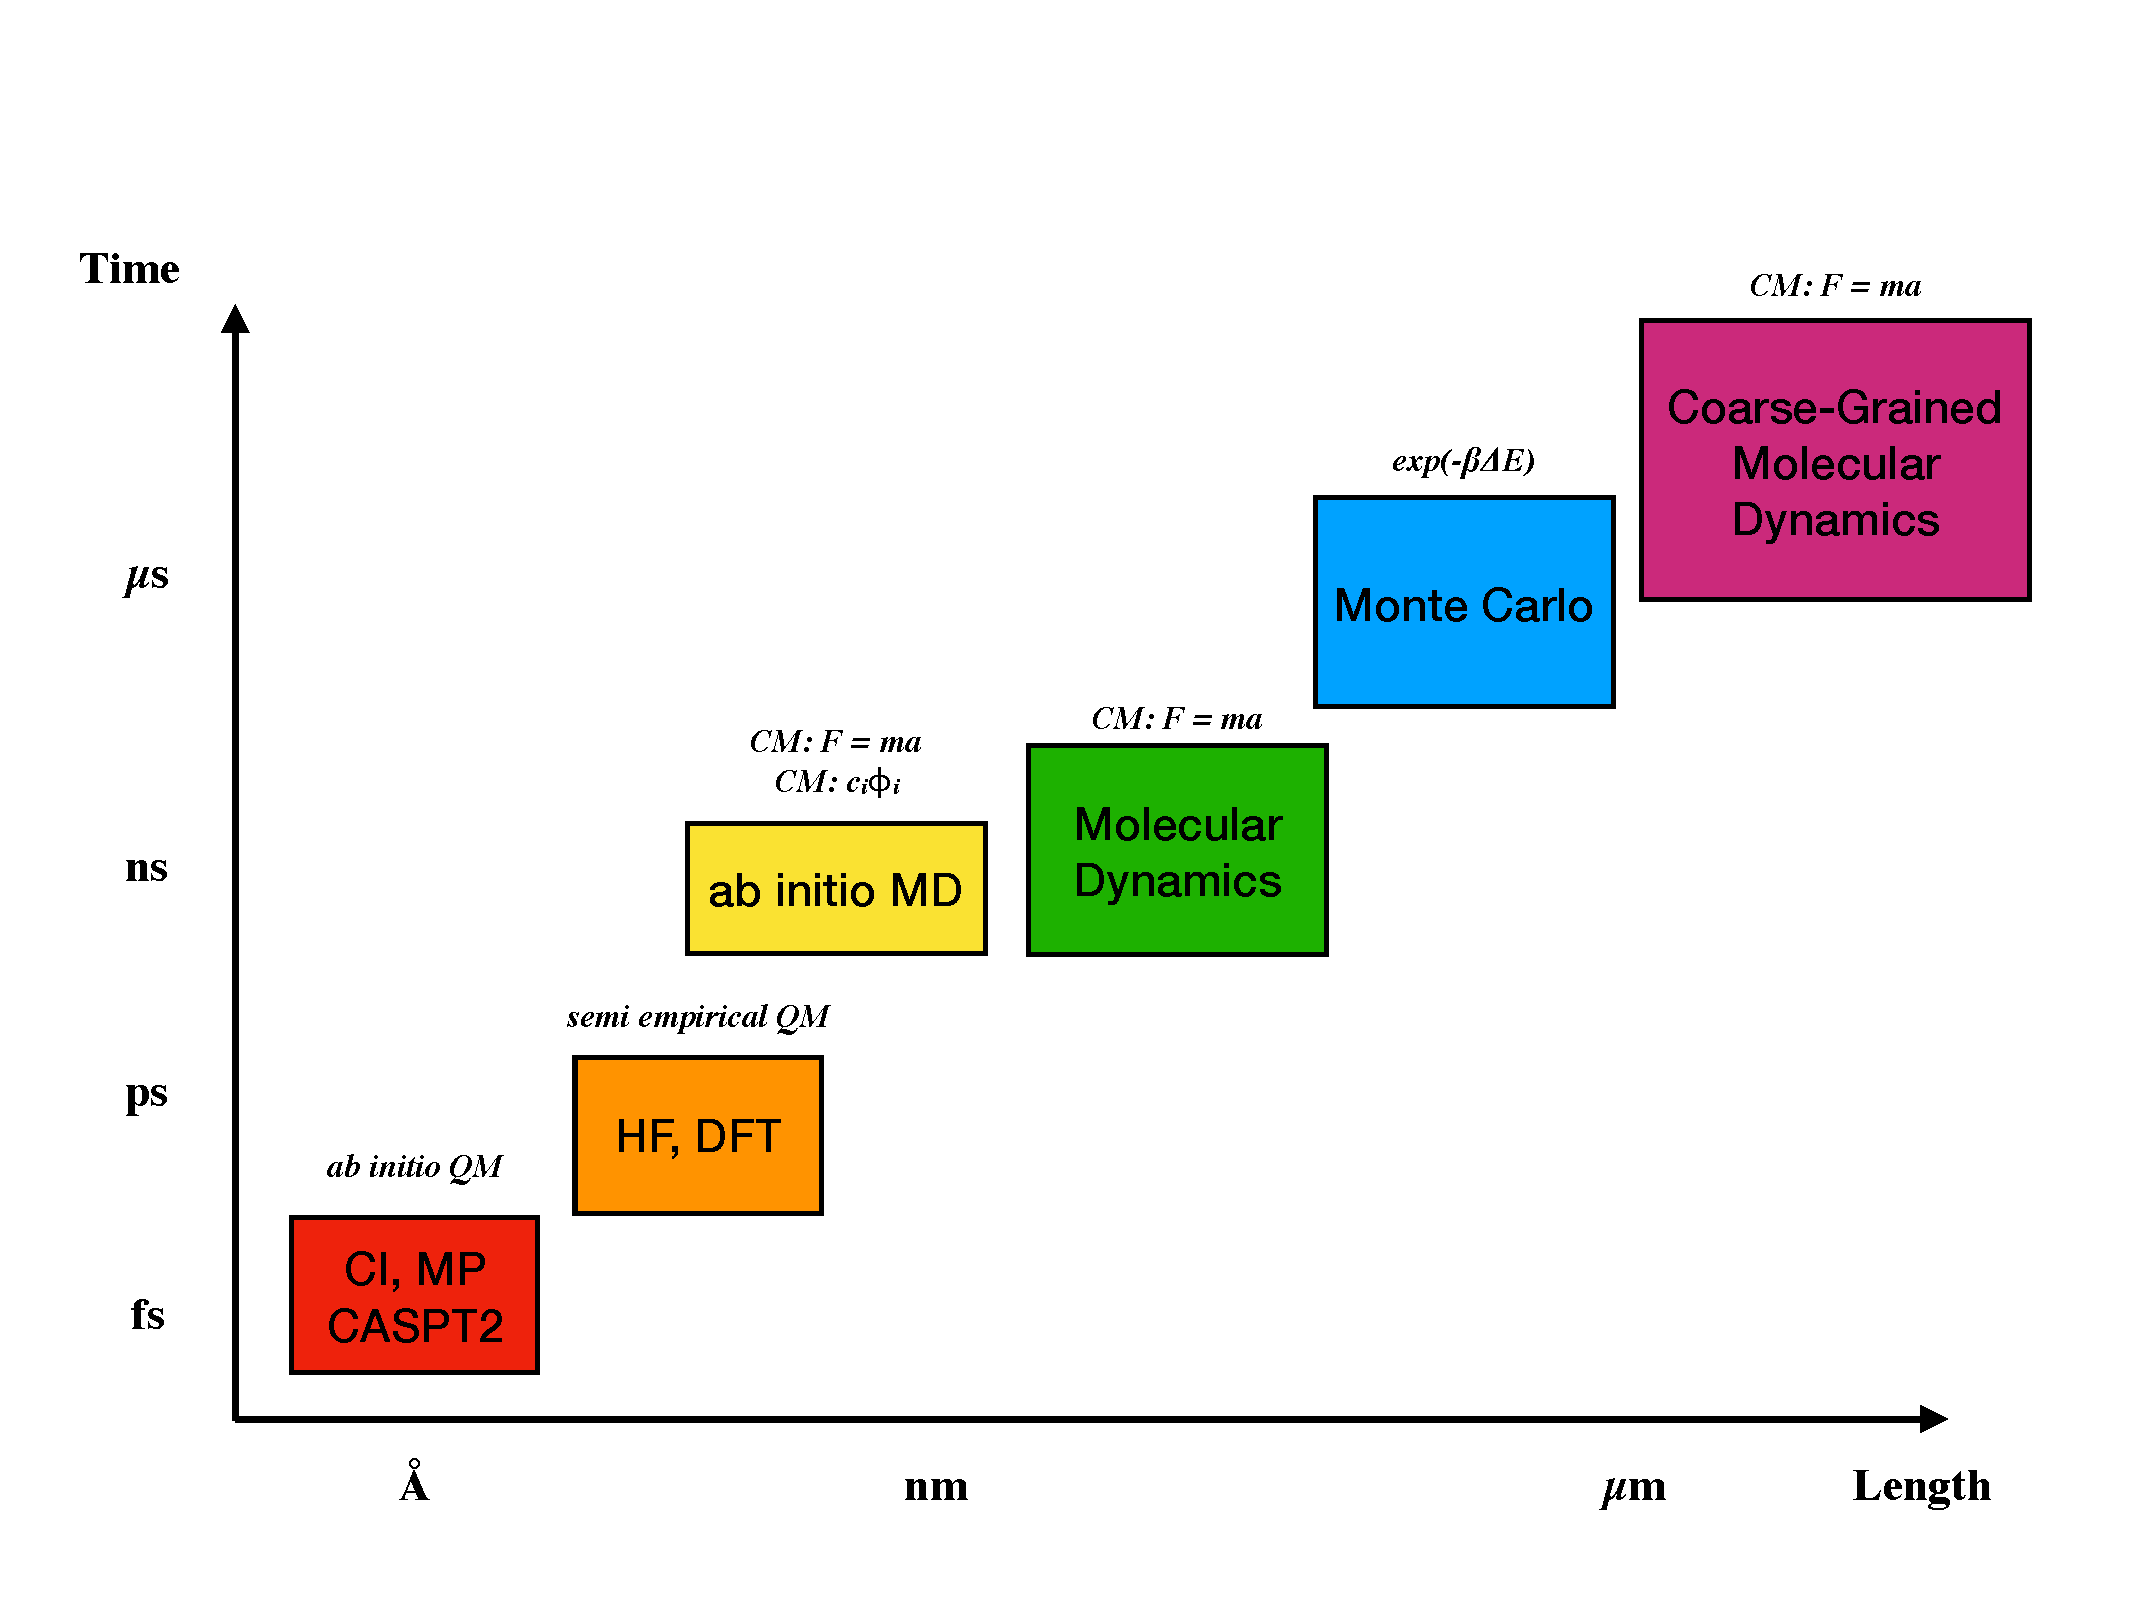
\includegraphics[width=\linewidth]{Figures/SimulationScale}
% \caption{\label{fig:SimulationScale} Different length scales in
%   numbers of molecules (here length of material) and corresponding
%   achievable simulation time for various molecular modeling
%   methodologies. High accuracy quantum mechanical methods (red and
%   orange) cannot simulate large numbers of molecules for long
%   times. Methods which reduce molecular detail and propogate by
%   classical mechanics (yellow and green) are able to achieve longer
%   simulation times for larger systems. Monte Carlo methods (blue)
%   remove the expense of computing dynamics altogether, and ultra
%   coarse-grained methods (violet) which approximate collections of
%   atoms as a single unit achieve even longer simulation times.}
% \end{figure}
In 1812, Pierre Simon Laplace published a manuscript entitled
\textit{A Philosophical Essay on Probabilities} detailing his system
of reasoning based on probabilities.\cite{LaplaceXX} Within this work,
he describes the notion of casual or scientific determinism, that is,
that all events are dictated by previously existing causes:
 
\begin{displayquote}
We may regard the present state of the universe as the effect of
its past and the cause of its future. An intellect which at a certain
moment would know all forces that set nature in motion, and all
positions of all items of which nature is comped, if this intellect
were also vast enough to submit these data to analysis, it would
embrace in a single formula the movements of the greatest bodies of
the universe and those of the tiniest atom; for such an intellect
nothing would be uncertain and the future just like the past would be
present before its eyes.
\end{displayquote}

This became known as Laplace's Demon, and a desire to confirm or
refute this claim was a significant driving force in the development
of statistical thermodynamics.  At the beginning of the 19th century,
concepts of irreversibility, entropy, and the second law of
thermodynamics suggested Laplace's Demon as being inaccurate.
Stochastic models for chaos theory and quantum mechanics provided
additional evidence against the claim, and it now agreed upon as
untrue.

Still, today we strive to achieve the premise that Laplace founded,
relinquishing the unobtainable asbolute predictablility of nature for
solvable representative models, stepping slowly towards understanding
the universe. We have replaced the `powerful intellect` with
computers, and develop algorithms to recursively solve these
complex models. Through computer simulations we are becoming more
proficient at understanding and predicting the world around us, from
the motion of planets, to the properties of molecules.

\section{Molecular Dynamics}
In a general defintion, molecular dynamics (MD) simulations involve
popogating molecules through time by Netwon's Second Law. The models
used to describe the molecules are often constructed using classical
mechanics, treating atoms as hard spheres and bonds between atoms
within a molecule as a spring. Charges are also handled classically,
and depending on the model the charges can be static (restricted to
some initial position), or dynamic, in which they allowed to move
around the molecule. While hybrid quantum / classical molecular
dynamics methods exist, we restrict ourselves here to the purely
classical case. In the following sections, I outline the basis of
classical molecular dynamics simulations. References for what is
presented comes from several excellent books which cover molecular
dynamics, from the classic text of Allan and Tildesey, to the modern
broad reaching work of Leach.\cite{AllanXX,LeachYY}

We begin by considering a many-body expansion of the configurational
potential energy $\mathscr{U}$ for an isolated collection of $N$ particles with
vector coordinates $\mathbf{r}^N$.
\begin{equation}\label{eq:potE}
\mathscr{U}(\mathbf{r}^N) = \sum_i U(\mathbf{r}_i) + \sum_{i<j}
U(\mathbf{r}_i,\mathbf{r}_j) + \sum_{i<j<k} U(\mathbf{r}_i,\mathbf{r}_j,\mathbf{r}_k) \dots + U(\mathbf{r}_1,\mathbf{r}_2,\mathbf{r}_3,\dots \mathbf{r}_N)
\end{equation}
Most commonly, the expansion is truncated at the two-body term as
higher order terms have proven computationally infeasible in the
past. However, with the development of faster computers, Paesani
\textit{et al.} has recently shown that incorporating higher order
terms leads to a more accurate water model.\cite{PaesaniXX} A more
detailed discussion on water models will be presented in Section
\ref{sec:WaterModels}; for now, we will restrict ourselves to a
many-body expansion up to the two-body term. We further restrict
ourselves to a potential where no dissapative forces act between
particles, from this, we can obtain the force on particle $i$.
\begin{equation}\label{eq:force}
\mathbf{F_i} = -\frac{\partial \mathscr{U}(\mathbf{r}^N)}{\partial \mathbf{r}_i}
\end{equation} 
Since the system of $N$ particles is isolated and there are no
dissapative forces, the total energy of the system will be
conserved. From Equation \eqref{eq:force} and Newton's Second Law the
accelerations for each of the $N$ particles follows.
\begin{equation}\label{eq:accel}
 m_i\mathbf{\ddot{r}}_i = -\frac{\partial \mathscr{U}(\mathbf{r}^N)}{\partial \mathbf{r}_i}
\end{equation}
Integrating Equation \eqref{eq:accel} once with respect to time gives
the momentum of the $N$ particles, and a second integration gives the
positions.

\subsection{Finite Difference Methods and Equations of Motion}
For particles described by a continous potential energy function, the
forces acting upon each of the $N$ particles will change every time a
single particles moves. Due to this, the motion of all particles are
coupled, giving rise to a many-body problem with no analytic
solution. Therefore, finite difference methods of integration must be
used in order to propogate the particles through time.

While there exist a large number of algorithms for propogating
particles, they are not all equal. The general idea for each method is
to take small steps through time ($\delta t$) by knowing the position
and momenta for each of the $N$ particles at a previous time
($t-\delta t$). Knowing these quantities, the forces are calculated
from the position, and the positions and momenta are updated
accordingly. This results in a new $\mathbf{r}^N$ configuration, and
the method iterates again.

The main difference between each integration scheme is what data is
stored between steps. In the \textit{Verlet} method, two sets of
positions are stored as well as a single set of accelerations. The
velocity terms do not appear explicitly but can be computed from the
two sets of positions. In the \textit{Leap Frog} method, the positions
and velocities are stored at a half-step difference. When the
positions are known at a half-step forward in time, the new velocities are
computed and `leap-frog` over the positions. While this method is an
improvement over the Verlet algorithm as the velocities are computed
directly, the positions and velocities are not known at the same time
without further calculations.

In our work, the \textit{velocity Verlet} method was implemented. In
this integration scheme the positions, velocities, and accelerations
are known at the same time. Given an initial set of positions at time
$t$, the accelerations $\mathbf{a}(t)$ can be computed from Equation
\eqref{eq:accel}. Together with the velocities at $t$, the future
values of these quantities can be determined.
\begin{equation}\label{eq:vv-r}
\mathbf{r}(t+\delta t) = \mathbf{r}(t) + \delta t \mathbf{v}(t) +
\frac{1}{2}t^2\mathbf{a}(t)
\end{equation}
\begin{equation}\label{eq:vv-v}
\mathbf{v}(t+ \delta t) = \mathbf{v}(t) + \frac{1}{2}\delta
t[\mathbf{a}(t) + \mathbf{a}(t + \delta t)]
\end{equation}
This method has to be implemented in three steps, as the accelerations
at times $t$ and $t + \delta t$ must be known to update the
velocities. In the first step, the positions are updated to
$t + \delta t$ using the velocities and accelerations at time $t$. In
the second step, the velocities at time $t + \frac{1}{2} \delta t$ are
computed.
\begin{equation}\label{eq:vv-v2}
\mathbf{v}(t+\frac{1}{2}\delta t) = \mathbf{v}(t) + \frac{1}{2}\delta t
\mathbf{a}(t)
\end{equation}
Forces are computed using the new positions $\mathbf{r}(t + \delta
t)$, and from these forces the new accelerations $\mathbf{a}(t +
\delta t)$ are determined. Lastly the velocities at time $t + \delta
t$ are computed by
\begin{equation}\label{eq:vv-v3}
\mathbf{v}(t+\delta t) = \mathbf{v}(t+\frac{1}{2}\delta t) +
\frac{1}{2}\delta \mathbf{a}(t + \delta t)
\end{equation}


\subsection{Time Averages and Ensemble Averages}
Consider a property $A$ that is dependent on the positions and momenta
of the $N$ particles in the system, then the instantaneous value of
the property $A$ can be expressed as
$A(\mathbf{r}^N(t),\mathbf{p}^N(t))$. As the positions and momenta of
the particles evolve, the value of $A$ fluctuates. During an
experiment, a \textit{time average} of $A$ is measured for a large
collection of particles. As the duration of the experiment increases,
the value of the measured property approaches the `true` value,
$A_{\mathrm{ave}}$.
\begin{equation}\label{eq:A-ave}
A_{\mathrm{ave}} = \mathrm{lim}_{\tau \to \infty} \frac{1}{\tau} \int_{t=0}^{\tau}
A(\mathbf{r}^N(t),\mathbf{p}^N(t))dt
\end{equation}

In theory, it is straightforward to compute the time averaged value of
$A$ from a computer simulation. As described previously, the positions
and velocities can be integrated through time, and for each
configuration of the system $A(\mathbf{r}^N(t),\mathbf{p}^N(t))$ could
be computed. The issue arises when considering a macroscopic number of
particles ($10^{23}$), as calculation of even the initial time step is
infeasible. Instead, we turn to statistical mechanics as a connection
between a microscopic system ($10^2 - 10^6$ particles) and the
macroscopic experimental observation. Here, instead of considering one
large system, we evolve a large number of replications of a smaller
systems simultaneously. The average value of the property from these
replicas is denoted as an \textit{ensemble average} with angle bars,
$\langle$~ $\rangle$.
\begin{equation}\label{eq:A-ens}
\langle A \rangle = \int \int d\mathbf{r}^N d\mathbf{p}^N
A(\mathbf{r}^N,\mathbf{p}^N) \rho
(\mathbf{r}^N,\mathbf{p}^N)
\end{equation}
Equation \eqref{eq:A-ens} is written with as double integral, although
more accurately this equation indicates $6N$ integrals, one for each
of the $3N$ position and $3N$ momentum coordinates of the $N$
particles. The second term in the integrand,
$ \rho(\mathbf{r}^N,\mathbf{p}^N)$, is the \textit{probability
  density} of the ensemble. It is a function which describes the
relative probability of observing a specific configuration and
distribution of momenta for the $N$ particles, given the energy of the
configuration. If one is able to compute $\langle A \rangle$ by
integrating over all possible configurations of the system, the
resulting ensemble average will be equal to the time average value
($A_{\mathrm{ave}} = \langle A \rangle$) by the \textit{ergodic
  hypothesis}. In practice, it is not often possible to integrate over
all possible configurations. Instead, convergence of the property
$\langle A \rangle$ is achieved once the system has explored a
sufficient amount of phase space.

\subsection{Calculation of Thermodynamic Properties}
As the particles evolve through time, there are several possible
thermodynamic properties which we may wish to compute. Among the
properties most commonly desired are the temperature and pressure.
The instantaneous temperature, $T$, of a collection of $N$ molecules
is described by their kinetic energy $K$ through the equipartition
theorem.
\begin{equation}\label{Temperature}
T = \frac{2}{fk_B}\Bigg( \sum_{i=1}^{N} \frac{1}{2} m_i {\bf v}_i^T \cdot {\bf v}_i +
\sum_{i=1}^{N_{\mathrm{linear}}+N_{\mathrm{non-linear}}}  \frac{1}{2} {\bf j}_i^T \cdot
\overleftrightarrow{\mathsf{I}}_i^{-1} \cdot {\bf j}_i  \Bigg)
\end{equation}

where $f$ is the total number of degrees of freedom in the system,
\begin{equation}
f = 3 N + 2 N_{\mathrm{linear}} + 3 N_{\mathrm{non-linear}} - N_{\mathrm{constraints}}
\end{equation}
$k_B$ is Boltzmann's constant, $N_{linear}$ is the number of linear
molecules, and $N_{non-linear}$ is the total number of non-linear
molecules in the system. The first sum includes the velocities of all
$N$ molecules, while the second sum is over those with angular
velocity $j_i$, and a moment of inertia
$\overleftrightarrow{\mathsf{I}}_i$.

The instantaneous pressure, $P$, of a collection of molecules can be
obtained through the virial theorem of Clausius. The \textit{virial},
$W$, is defined by
\begin{equation}\label{eq:virial}
W = \sum_i^N r_i\dot{p}_{r_i}
\end{equation}
where $r_i$ is a coordinate such as the $x$ or $y$ dimension, and
$\dot{p}_{r_i}$ is the first time derivitive of momentum, or force,
along that coordinate. The virial theorem of Clausius states that the
virial is equal to $-3Nk_BT$.

For an ideal gas, the molecules composing the gas only interact with
the walls of the container. Therefore, the only forces present in the
system are due to those between the gas and the container. In this
case, the virial becomes $-3PV$ directly from the ideal gas law
$PV=-Nk_BT$. We can consider a system of interacting particles as a
perturbation from the ideal gas case, where the virial for the
interacting system would be the ideal gas virial plus a contribution
due to the interactions of the particles. 
\begin{equation}\label{eq:virial2}
W = -3PV + \sum_i^N \sum_{j\neq i}^N r_{ij} \frac{dU(r_{ij})}{dr_{ij}} = -3Nk_BT
\end{equation}
Here we have considered a potential consisting of only two-body
interactions, although expansion to consider higher-order terms is
straightforward. If we instead write Equation \eqref{eq:virial2} in terms
of the force between particles $i$ and $j$, ($f_{ij}$), we obtain the
following expression for the pressure.
\begin{equation}\label{eq:virial3}
P = \frac{1}{V}\Big[Nk_BT - \frac{1}{3} \sum_i^N \sum_{j\neq i}^N
r_{ij} f_{ij}\Big]
\end{equation}

These are just two of many thermodynamic properties one may wish to
compute as a simulation evolves. The problem of writing expressions
for the desired properties in terms of particle positions and
velocities lies at the heart of the matter. Once established, solving
the equations at regular intervals of simulation time becomes
straightforward. As an interesting final remark on this section, we
note that while two identical collections of particles (with the exact
same set of positions and velocities) evolving under different
potential energy functions will reproduce the same temperature for
that configuration, the associated pressures (and many other
thermodynamic properties) will be different. Therefore, we should
expect collections of the same molecules (\textit{e.g.} water)
described under different potential energy functions or parameters, to
result in vastly different thermodynamic properties.

\subsection{Molecular Forcefields}
Having established how to propogate particles through time using MD
simulations, we turn our focus next to the problem of developing an
accurate representation for the interactions between molecules, more
commonly known as a forcefield. Generally, the functional form of the
forcefield is structured as a balance between accurately capturing the
pertinent physics and what is feasible in computing time. Here, we
present functional forms for forcefields commonly used, followed by a
discussion of suitable parameters in a brief overview of the large
body of literature surrounding water models.

Due to computational expense, it is common to truncate the many-body
expansion of the potential energy to include only the one-body and
two-body interaction terms, and consider only those two-body terms
which are pairwise additive. That is, the potential in Equation
\eqref{eq:potE} becomes,
\begin{equation}\label{eq:potPair}
\mathscr{U}(\mathbf{r}^N) = \sum_i^N U(\mathbf{r}_i) + \sum_{i<j}^N U(r_{ij})
\end{equation}
where $\mathbf{r}_i$ is the absolute position of particle $i$, and
$r_{ij}$ is the scalar distance between particles $i$ and $j$,
$r_{ij} = | \mathbf{r}_i - \mathbf{r}_j|$. This may seem like an
extreme restriction on the potential, however, we will see models of
this structure still perform quite well. 

The one-body term in Equation \eqref{eq:potPair} accounts for any
external forces on the particles, such as an external electric
field. Their interaction with the field depends on the particle's
absolute position in that field, not the relative distance between the
other particles. In the absence of external forces, Equation
\eqref{eq:potPair} reduces to just the two-body pairwise additive
term, and the potential only depends upon the relative distance
between particles. Generally, these terms fall into one of two
categories, bonded and non-bonded interactions.

\subsubsection{Bonded Interactions}
There are three bonded terms (often referred to as short-ranged
interactions) which deserve discussion. Bonds between two atoms in a
molecule, bends between three centrally connected atoms, and torsions
between four consecutively bonded atoms. Bonds are often treated as
harmonic oscillators, with a spring constant $k_{ij}$ set to mimic the
stiffness of the bond and equilibrium distance set to the bond length
$r_{ij}^0$. The spring constant is determined from the frequency of
the bond $\omega$ and the reduced mass $\mu_{ij}$ of the two atoms in the
bond.
\begin{equation}\label{eq:kij}
\omega = \sqrt{\frac{k_{ij}}{\mu_{ij}} }
\end{equation}

\begin{equation}\label{eq:bonds}
U_{bond}(r_{ij}) = \frac{1}{2} k_{ij} (r_{ij} -r_{ij}^0)^2
\end{equation}

Similarly, bends within a molecule are also treated as a harmonic
oscillator, with spring constant $k_{\theta_{ijk}}$ and equilibrium bend
angle $\theta_{ijk}^0$. However, while the bonding potential is a
function of the distance between particles $i$ and $j$, the bending
potential is more succinclty written as a function of the angle formed between three
consecutively bonded atoms $i$, $j$, and $k$,
\begin{equation}\label{eq:bend}
\theta_{ijk} = \mathrm{cos}^{-1}\Bigg(\frac{\mathbf{r}_{ji} \cdot
  \mathbf{r}_{jk}}{|r_{ji}|~|r_{jk}|}\Bigg)
\end{equation}
where particle $j$ is the central atom. 
\begin{equation}\label{eq:bend2}
U_{bend}(\theta_{ijk}) = \frac{1}{2} k_{\theta_{ijk}} (\theta_{ijk} -
\theta_{ijk}^0)^2
\end{equation}

A torsion describes a rotation of groups about a central bond, and is
often expressed in terms of a cosine expansion.
\begin{equation}\label{eq:torsion}
U_{torsion}(\phi_{ijkl}) = c_1[1+\mathrm{cos}\phi_{ijkl}] + c_2[1-\mathrm{cos}(2\phi_{ijkl})]+c_3[1+\mathrm{cos}(3\phi_{ijkl})]
\end{equation}
Here, the angle $\phi_{ijkl}$ is defined as
\begin{equation}\label{eq:torsion2}
\mathrm{cos}\phi_{ijkl} = (\mathbf{\hat{r}}_{ij} \times
\mathbf{\hat{r}}_{jk}) \cdot (\mathbf{\hat{r}}_{jk} \times
\mathbf{\hat{r}}_{kl})
\end{equation}
and the coefficients $c_1$, $c_2$, and $c_3$ are terms describing the
barrier for transitioning from a \textit{cis} to a \textit{trans}, or \textit{staggered} to
\textit{eclipsed} conformations.

\subsubsection{Non-bonded Interactions}
In 1924, J. E. Lennard-Jones proposed a pairwise additive
non-bonded potential for a system of soft-spheres.
\begin{equation}\label{eq:LJ}
U_{\mathrm{LJ}}(r_{ij}) = k\epsilon_{ij}\Bigg[ \Big( \frac{\sigma_{ij}}{r_{ij}}\Big)^n - \Big(\frac{\sigma_{ij}}{r_{ij}}\Big)^m\Bigg]
\end{equation}
where
\begin{equation}\label{eq:LJ2}
k = \frac{n}{n-m} \Big(\frac{n}{m}\Big)^{m/(n-m)}.
\end{equation}
With this simple model, Lennard-Jones was able to account for both
short-ranged repulsive forces as well as long-range attractive
forces. The short-ranged forces are important to keep a collection of
particles from collapsing in on itself, while the long-range forces
prevents the collection of particles disintegrating. Since the leading
term in London's theory on dispersion forces goes at $1/r^6$, the
long-range term is chosen to mimic this behavior $m=6$. While there is
no physical justification for it, the short-ranged attraction term is
often set to $n=12$ primarily due to ease of computation. With these
values for $m$ and $n$ the resulting Lennard-Jones model becomes
\begin{equation}\label{eq:LJ3}
U_{\mathrm{LJ}}(r_{ij}) =
4\epsilon_{ij}\Bigg[\Big(\frac{\sigma_{ij}}{r_{ij}}\Big)^{12}-\Big(\frac{\sigma_{ij}}{r_{ij}}\Big)^{6}\Bigg].
\end{equation} 
The remaining two parameters to the model are $\sigma_{ij}$, the distance
at which $U_{\mathrm{LJ}}(r_{ij})$ goes to zero, and $\epsilon_{ij}$, the potential
energy minimum which is located at $r_{ij} = \sqrt[6]{2}\sigma_{ij}$. While the
number and locations of Lennard-Jones sites within water models vary,
the parameter $\sigma$ is commonly taken to be the molecular diameter
and $\epsilon$ is often tuned to reproduce a certain region of the
phase diagram. Interactions between different types of particles
requires a mixing of the parameters $\sigma$ and $\epsilon$. These are
normally determined by the Lorentz-Berthelot mixing rules, where
$\sigma_{ij}$ is determined by an algebraic mean 
\begin{equation}\label{eq:sigma}
\sigma_{ij} = \frac{1}{2} [\sigma_{ii} + \sigma_{jj}]
\end{equation}
and $\epsilon_{ij}$ is taken as the geometric mean of $\epsilon$ for
particles $i$ and $j$. \cite{paper}
\begin{equation}\label{eq:epsilon}
\epsilon_{ij} = \sqrt{\epsilon_{ii}\epsilon_{jj}}
\end{equation}


A second non-bonded interaction we must consider is the appropriate
treatment of charged particles. Commonly, molecular mechanics
forcefields represent molecular charges as point charges on atomic
sites, coupled with short-ranged Lennard-Jones repulsions to prevent
molecules from collapsing onto one another. While there are many
implementations of how to compute these interactions, Coulomb's law is
at the heart of the methods.
\begin{equation}\label{eq:coulomb}
U_{\mathrm{charge}}(r_{ij}) = \sum_{ij}\frac{q_i q_j e^2}{4 \pi \epsilon_0
  r_{ij}}
\end{equation}
Here, $q_i$ and $q_j$ are the charges on particles $i$ and $j$, $e$ is
the charge of an electron, and $\epsilon_0$ is the permittivity of
free space. 

For a system of $N$ molecules, the number of bonded terms goes as $N$
but the number non-bonded interactions as $N^2$. Due to this,
computing the non-bonded interactions is often the most
computationally expsive part of the simulation. The Lennard-Jones
interaction, however, fall of quite rapidly ($r^{-6}$) and the
potential at $r_{ij} = 2.5\sigma_{ij}$ is just $1 \%$ of its value at
$r_{ij} = \sigma_{ij}$. Meanwhile, the long-ranged $r^{-1}$ decay of
electrostatic interactions can have significant value at distances as
large as the simulation cell. These interactions are quite problematic
and will be addressed in the following paragraphs. However, we will
first discuss adding a cutoff to the potential, a method commonly
used to save computation time.

% Make cutoff small enough that particle doesn't see its own
% image. Neighbor-lists make cutoffs worthwhile, otherwise we would have
% to compute all pairwise distance each timestep to determine if we
% should compute potential and forces or not. In larger systems, a cell
% index method can be used where the molecules are cast into mini cells,
% and then neighbor lists are constructed from the 26 cells surrounding
% the cell in question (total of 27 cells then). Sorting molecules is on
% order $N$, and sorting neighbors is cheap as long as the total number
% of cells is greater than 27.

When using a cutoff radius, the potential is evaluated as normal for
distances less than the cutoff, and set to zero for objects outside
the cutoff. This introduces discontinuities in the potential and thus
the force calculations. One way around this is to shift the potential
by its value at the cutoff.  The additive constant vanishes upon
taking the derivative to compute the forces, and energy conservation
is better than with the unshifted potential. However, there is still a
problem of a discontinuity in the force with this method. A second
solution is to use a switching function, to smoothly transition the
potential to zero at the cutoff.

% Switching functions can take several forms, one
% such example is the following polynomial
% \begin{equation}
% v'(r) = v(r)\Big[1-2\Big(\frac{r}{r_c}\Big)^2 + 
% 4\Big(\frac{r}{r_c}\Big)^4 \Big]
% \end{equation}
% The switching function has a value of $1$ at $r=0$ and $0$ at
% $r = r_c$. Switching functions are normally implemented at some
% distance close to the cutoff, so that only a small amount of the
% potential is perturbed. This prevents asparious affects such as
% deviation from equilibrium structures. Need the first derivative of
% the switching function at the end points to be zero to ensure the
% forces approach zero smoothly, and second derivitives to be zero for
% stability of integration algorithm. 
% \begin{equation}
% S(r) = c_0 + c_1\Big[\frac{r-r_l}{r_u-r_l}\Big] +
% c_2\Big[\frac{r-r_l}{r_u - r_l}\Big]^2
% + c_3\Big[\frac{r-r_l}{r_u-r_l}\Big]^3 +
% c_4\Big[\frac{r-r_l}{r_u-r_l}\Big]^4 +
% c_5\Big[\frac{r-r_l}{r_u-r_l}\Big]^5
% \end{equation}
% The set of coefficients that satisfies the derivative stipulations are
% $(c_0 = 1, c_1 = 0, c_2 = 0, c_3 = -10, c_4 = 15, c_5 = -6)$.

Interactions that decay no faster than $r^{-n}$ where $n$ is the
dimensionality of the system can pose a problem in that they may not
converge for distances greater than the size of the simulation
box. Charge-charge interacations go as $r^{-1}$, and therefore are
quite problematic. There have been several methods suggested to handle
this issue, the most famous of which is the method presented by Ewald
in 1921. The Ewald Sum requires replicas of the simulation cell for
computation of $U_{charge}(r_{ij})$. These charges are then wrapped by
a Gaussian of opposite charge, creating a mask around the
charges. Doing so requires two corrections to be made; first, an
oppositely charged Gaussian must also be added for each one introduced
around a charge. Secondly, since the Gaussians interact with
themselves, a self correction piece must be added as well. Depending
on the material being modeled, a dipole correction might also need to
be added. The charges and the Gaussians wrapped about them are added
up in real space, while the oppositely charged Gaussians are added in
reciprocal space. This method is computationaly very expensive,
however, it is the most accurate way of computing the charge-charge
interactions in molecular simulation. 

An alternative approach to the demanding Ewald Sum is the method first
developed by Wolf \textit{et al.}, and later expanded upon by Fennel
and Gezelter.\cite{Fennell2006} This method combines shifting the
potential as described above with a dampening of the electrostatic
interactions in a similar fashion as the Ewald Summation. The first
key observation is that the electrostatic interactions are shorter
ranged than $r^{-1}$ in condensed phases. Wolf \textit{et al.}
observed that creating a neutral cutoff sphere resulted in a
good conservation of energy. We begin with the standard shifted potential,

\begin{equation}
V_\textrm{SP}(r) =      \begin{cases}
v(r)-v_\textrm{c} &\quad r\leqslant R_\textrm{c} \\ 0 &\quad r >
R_\textrm{c}  
\end{cases},
\label{eq:shiftingPotForm}
\end{equation}
and expand on this to the shifted force,
\begin{equation}
V_\textrm{SF}(r) =      \begin{cases}
v(r)-v_\textrm{c}-\left(\frac{d v(r)}{d r}\right)_{r=R_\textrm{c}}(r-R_\textrm{c
})
&\quad r\leqslant R_\textrm{c} \\ 0 &\quad r > R_\textrm{c} 
                                                \end{cases},
\label{eq:shiftingForm}
\end{equation}

which guarantees the potential and forces smoothly go to zero at the
cutoff radius, $R_\textrm{c}$. Wolf \textit{et al.} observed that when
the potential is taken to be the Coulomb potential, Equation
\ref{eq:coulomb}, the calculated Madelung energies fluctuated around
the analytic value with increasing size of the cutoff radius, with a
slow decay towards the expected value. Therefore, to accelerate the
convergence of the expected energies, a dampening function was
introduced resembling the effective screening of the oppositely
charged Gaussians in the Ewald summation. Doing so, Fennell and
Gezelter arrived at the following damped shifted force,

\begin{equation}
\begin{split}
V_\mathrm{DSF}(r) = q_iq_j\Biggr{[} & \frac{\mathrm{erfc}\left(\alpha r \right)}{r} -\frac{\mathrm{erfc}\left(\alpha R_\mathrm{c} \right) }{R_\mathrm{c}} \\
 & \left. +\left(\frac{\mathrm{erfc}\left(\alpha
R_\mathrm{c}\right)}{R_\mathrm{c}^2}+\frac{2\alpha}{\pi^{1/2}}\frac{\exp\left(-\alpha^2R_\mathrm{c}^2\right)}{R_\mathrm{c}}\right)\left(r-R_\mathrm{c}\right)
\right] \quad r\leqslant R_\textrm{c} 
\label{eq:DSFPot}
\end{split}
\end{equation}
where $efrc$ is the complimentary error function with dampening
parameter $\alpha$. Taking the derivative of this damped shifted force
potential will lead to the following expression for forces,
\begin{equation}
\begin{split}
F_\mathrm{DSF}(r) =
q_iq_j\Biggr{[}&\left(\frac{\textrm{erfc}\left(\alpha r\right)}{r^2}+\frac{2\alpha}{\pi^{1/2}}\frac{\exp{\left(-\alpha^2r^2\right)}}{r}\right) \\ &\left.-\left(\frac{\textrm{erfc}\left(\alpha R_{\textrm{c}}\right)}{R_{\textrm{c}}^2}+\frac{2\alpha}{\pi^{1/2}}\frac{\exp{\left(-\alpha^2R_{\textrm{c}}^2
\right)}}{R_{\textrm{c}}}\right)\right] \quad r\leqslant R_\textrm{c}.
\label{eq:DSFForces}
\end{split}
\end{equation}
Fennell and Gezelter have shown that the damped shifted force method
gives nearly identical results as compared with the smooth particle
mesh Ewald method on a variety of commonly simulated
systems.\cite{Fennell2006}

\subsection{Boundary Conditions}
Having discussed how to evolve particles positions and momenta through
time under a classical potential, we now focus on the problem of how
to simulate a tractable number of particles. Consider an open (but
isolated) system of particles. The cluster would be exposed to vacuum
in all three dimensions, and depending on the strength of the
intermolecular interactions, the cluster could condense into a sphere
or slowly dissipate into a gas. If we were interested in simulating a
liquid and had incorporated an appropriate intermolecular potential,
the vacuum exposed droplet would be a poor representation of a bulk
liquid.

A naive approach to fix this problem would be to simulate a large
cluster of molecules and only probe the properties of the interior
molecules. This is both inefficient and potentially inaccurate, as
determining when a cluster is `large enough` for the interior
molecules to recover bulk liquid behavior is open to
interpretation. An efficient solution to this problem is to impose
boundary conditions on the system. While the type of boundary
condition imposed can depend on the type of material being simulated,
cubic or parallelepiped periodic boundary conditions are the most
common. In these methods, the system of particles is
effectively replicated around the initial simulation cell. If a
particle leaves the simulation cell (\textit{e.g.} through the
positive $x$ dimension) then one of the images of the particle will
enter the cell through the opposite wall (from the negative $x$
dimension).

In Figure \ref{fig:PBC}, a two-dimensional representation of cubic
periodic boundary conditions shows how the true simulation cell (in
blue) has a constant number of particles (red circles). As a particle
leaves the initial cell an image of itself enters through one of the
ghost cells surrounding the box. This is achieved by either wrapping
the position of each particle back to the initial cell after each
timestep, or by computing the potential energy and force calculations
using the ghost images. Notice that the nearest particles within the
cutoff radii, $r_{\mathrm{cut}}$, may be an image of a particle in one
of the ghost cells. Using this method, it is possible to simulate a
bulk fluid (or more generally a bulk material) using a tractable
number of particles.

\begin{figure*}
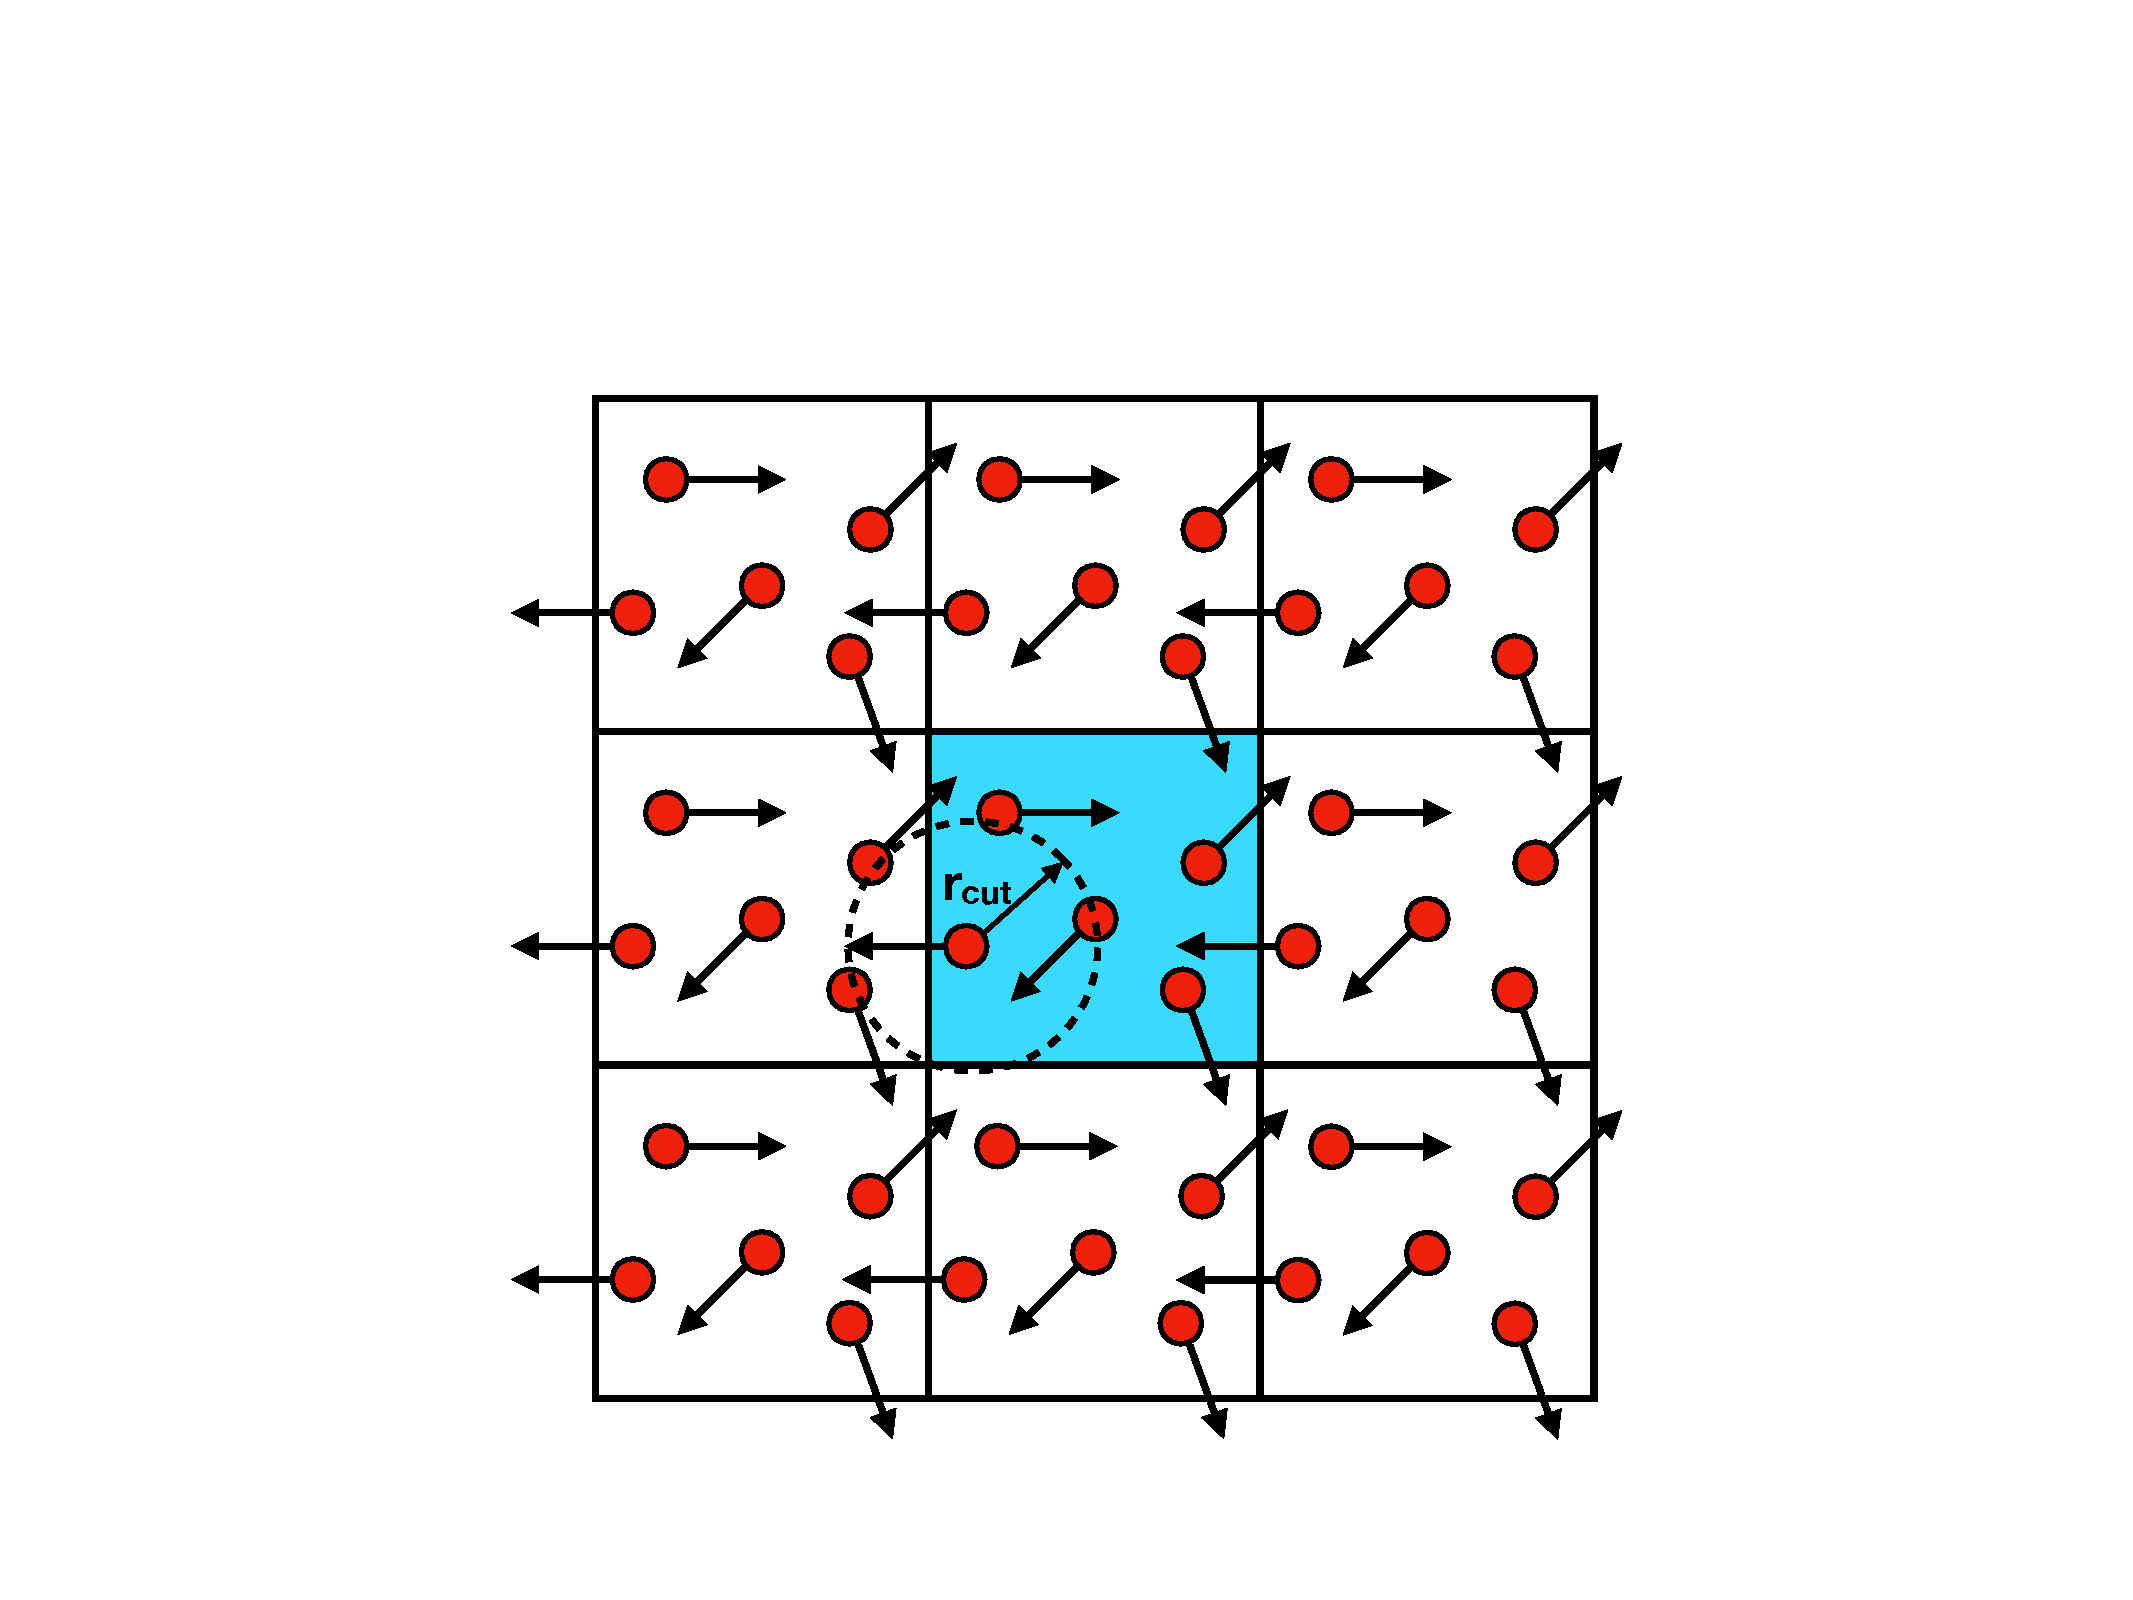
\includegraphics[width=\linewidth]{Figures/PBC}
\caption{\label{fig:PBC} Periodic boundary conditions and minimum
  image calculation. The central blue cell is the only simulation cell
  maintained by computation. Molecules (red circles) are free to move
  throughout space uninhindered. When a molecule leaves the blue
  simulation cell, one of its ghost images enters the cell from one of
  the neighboring cells. This is achieved by computation of
  interactions of a molecule with its nearest neighbors within a
  cutoff radius of $r_{\mathrm{cut}}$. Note these molecules may not
  necessarily be located within the same simulation cell as the
  molecule of interest.}
\end{figure*}

Utilizing periodic boundary conditions does pose one potential
problem. There is the possibility that a particle could interact with
an image of itself, if the unit cell length is not large compared to
$r_{\mathrm{cut}}$. Also, while using these methodologies capture
short wavelength events quite well, it is impossible to observe a
phenomena with fluctuations or wavelengths larger than the unit cell
dimensions. This includes events near liquid-gas critical points,
observing phase transitions, and long-wavelength plasmons. However,
unnecessarily large unit cells require an increasing number of
particles in the simulation, and resulting computational times
intractable.



\subsection{Water Models}\label{sec:WaterModels}
An investigation of the properties and dynamics of water anywhere in
the phase diagram cannot be conducted without first critically
analyzing the model proposed for the study. After almost 50 years of
simulating water, we are still optimizing and searching for geometries
and distributions of charges, potential sites, mass sites, and many
other parameters which will reproduce the phase diagram of water in
closer detail. However, in this time we have learned much about the
rich behavior and characteristics of water through molecular
simulations. 

In this section we present a short review over the large body of
literature surrounding water models for molecular simulations. The
list of water models presented here is by no means complete, nor the
analysis of these models exhaustive. There are a number of excellent
reviews on these topics, from the early reviews of
Brodsky\cite{Brodsky1996}, Wallqvist and Mountain\cite{Wallqvist1999},
Finney\cite{Finney2001}, and Guillot\cite{Guillot2002}, to the more
recent works of Ouyang\cite{Ouyang2015}, Cisneros\cite{Cisneros2016},
Gallo\cite{Gallo2016}, and Brini\cite{Brini2017}. We would be remiss
if we also did not include the significant contributions from the
Unversidad Complutense Madrid, namely, the extensive work of Vega,
Abascal, Conde, Sanz, and
MacDowll.\cite{MacDowell2004,Vega2005,Vega2005c,Abascal2007,Abascal2007a,Abascal2007b,Abascal2007c,Vega2009,Vega2011,Vega2011a,Vega2015}
Lastly, we must include the expansive catalog of Martin
Chaplin.\cite{Chaplin2018}

The first simulations of water were performed in 1969 by Barker and
Watts,\cite{Barker1969} and shortly thereafter by Rahman and
Stillinger in 1971\cite{Rahman1971} using the Ben-Naim Stillinger
potential\cite{Ben-Naim1972}. These inaugural investigations used
rigid, non-polarizable models for water, consisting of Lennard-Jones
and charge sites describing the intermolecular interactions, evolving
according to classical mechanics. Soon thereafter, Rahman and
Stilleger proposed the five-site ST2 model, which better captured the
density maximum for liquid water, and whose distribution functions
more accurately matched x-ray scattering data.\cite{Stillinger1974}

Since this time, hundreds of water models have been proposed and
characterized.\cite{Chaplin2018} These range from computationally
expensive models such as the SWM-4DP\cite{Lamourex2003},
TIP4P-FQ\cite{Rick1994}, DPP2\cite{Kumar2010},
TTM3-F\cite{Fanourgakis2008}, and AMOEBA\cite{Ren2003,Ren2004} models,
which have moved beyond point charges and the pairwise additive
approximation and allow for anisotropic multipole polarizations, while
others have attempted to make large scale simulations more feasible by
collapsing the water molecule onto a single interaction
site\cite{Liu1996,Tan2003,Fennell2004}.

\subsubsection{Classes of Water Models}
Most commonly, water models are categorized by the number of
interaction sites and divided into subcategories by the types of
interactions described within the potential. Three, four, five, and
six site models are prevalant in the literature, although
computational expense increases with the number of interaction sites
($s$); as the number of non-bonded terms for $N$ molecules goes as
$s^N$. In reality, the number of interaction pairs needed to be
calculated are slightly less than $s^N$ as some of the interaction
sites are exclusively Lennard-Jones or charge sites.

Here, we will focus on non-polarizable models, that is, models where
the charge distribution is held fixed and not allowed to move around
the molecule. Similarly, we will restrict ourselves to rigid models,
where the OH bonds and HOH bends are held fixed in space. While there
are several models which propogate these degrees of freedom, such as
the SPC/f\cite{Ferguson1995}, SPC/Fw\cite{Wu2006}, and
TIP4P/2005f\cite{Gonzalez2011} models, limiting our discussion to
models which exclude these degrees of freedom will provide a more
similar comparison. XXX

The two most common three site models are Berendsen's
SPC/E\cite{Berendsen1987} and Jorgenson's TIP3P\cite{Jorgenson1983}
models. In both cases, the interaction sites are set to the atomic
positions, with positive charges on the two hydrogens and a negative
charge located on the oxygen. A Lennard-Jones interaction is also
defined on the oxygen site to prevent the molecules from collapsing
onto one another. The SPC/E model is a reparameterization of the
SPC\cite{Berendsen1981} model, where a self-energy correction was
included correcting the average polarization. With this correction,
the model more accurately reproduces the second neighbor peaks in the
pairwise radial distribution functions, as well as the density and the
diffusion at ambient conditions.\cite{Berendsen1987}

While attempting to determine the total internal energy of a water
molecule, Bernal and Fowler found that in order to reproduce the
observed dipole moment of water, they had to shift the negative charge
off of the oxygen towards the hydrogens along the HOH
bisector.\cite{Bernal1993} Following this idea, Jorgenson \textit{et
  al.} developed a four site water model, moving the negative charge
from the oxygen to a massless site along the HOH bisector. The
resulting TIP4P model more accurately reproduced oxygen-oxygen
diffraction data than the TIP3P model.\cite{Jorgenson1983} The four
site model was also found to have the correct density of liquid water
at 298.15~K and 1~atm. 

Due to the success of the TIP4P model, the four site structure has
been replicated and parameters refined spawning a large number of
models, including the TIP4P/Ew\cite{Horn2004},
TIP4P/2005\cite{Abascal2005a}, and TIP4P/Ice\cite{Abascal2005}
models. Simulations involving biomolecules often involve a large
number of charged species, as such, the TIP4P/Ew model is a
reparameterization of the TIP4P model for use with Ewald summation
methods. The TIP4P/2005 model was developed as a general purpose model
for condensed phases of water. Reparameterization was achieved using a
large amount of data from across the phase diagram. These data
include a fit of the temperature of maximum density, stability of
several ice polymorphs, the enthalpy of vaporization, and the density
of the liquid at ambient conditions. The resulting model gives good
agreement over a large span of the phase diagram, and has recently
been suggested as being the most accurate rigid non-polarizable model
to date.\cite{Vega2011a} 

In contrast to the parameterization of the TIP4P/2005 model where the
goal was to create a single model which spans much of the phase
diagram accurately, the TIP4P/Ice model was developed targeting the
properties of ice. The model was parameterized by fitting the equation
of state and selected points of the solid / liquid coexistence curves,
as well as the solid / solid coexistence curves. The model gives
excellent agreement for the melting temperature of ice-I$_\mathrm{h}$,
with T$_\mathrm{m} = $272.2~K. 

The category of five site models includes the ST2 model originally
proposed by Stillinger and Rahman in 1972\cite{Stillinger1974}, the
TIP5P model of Mahoney and Jorgensen\cite{Mahoney2000}, and its
reparameterization for use with Ewald summation methods (TIP5P/Ew) by
Rick.\cite{Rick2004} In the five site models, the negative charge has
moved out of the HOH plane, and is now distributed on the far side of
the oxygen mimicing the electron lone pairs. The positive charges are
located on the hydrogn sites, and the Lennard-Jones position is placed
on the oxygen atom. The TIP5P model is observed to reproduce the
density maximum of water around 4\degree~C at 1~atm, and the
dielectric constant was found to be 81 $\pm$ 1.5 at 25\degree~C, in
good agreement with the experimentally known value (78.4). While these
and other properties predicted by the TIP5P model agree well with
experimental results, it has recently been shown that when one
considers performance of the model for a large number of properties,
the three site SPC/E and four site TIP4P/2005 water models outperform
the costly five site model. 

While there are not many six site rigid nonpolarizable water models,
one bares worth mentioning. The NE6 model of Nada and van der Eerden
is the same as the five site models described above, with the addition
of a massless charged site along the HOH bisector.\cite{Nada2003a}
This charge is taken to be negative, however, the total molecule is
constrained to be neutral. The model was parameterized for simulations
involving ice and liquid near the melting point, and parameters were
determined from derivatives of the free energy of ice and water, as
well as the volumes of the same systems. Proton-disordered
ice-I$_\mathrm{h}$is the stable structure at the melting point for the
resulting NE6 model. The melting point was determined to be
271~$\pm$~9~K by Nada and van der Eerden, in good agreement with the
experimentally observed 273.15~K.

\subsubsection{Parameterizing Water Models}
After selecting the number of potential sites for a water model, the
next task is determining the interaction parameters associated with
each of those sites. Commonly, water models are parameterized in one
of two distinct ways, through \textit{ab. initio} calculations or
matching emperical evidence. In the first method, high level quantum
mechanical calculations are performed on small clusters of water
molecules. From these, forces, stresses, and energies are obtained and
fit using a pairwise (or higher order) function to describe the
energy. In the second method, parameters for the interaction sites are
determined by iterative fitting against chosen experimental results,
such as the density or coexesistence temperatures. A set of
interaction parameres are chosen, such as the charges ($\mathrm{q}_O$
and $\mathrm{q}_H$) and Lennard-Jones parameters ($\epsilon_O$ and
$\sigma_O$), and the resulting behavior of the water model is
recorded. The parameters are then iteratively changed until
convergence with the experimental data is achieved. 

Izadi and Onufriev have recently argued that the accuracy limit of the
rigid non-polarizable three and four site water models has been
achieved.\cite{Izadi2014,Izadi2016} In their initial work, they
iteratively solved for the optimal charge distribution for a four site
model.\cite{Izadi2014} The resulting OPC model reproduced bulk
properties more accurately than many other existing models. In
addition, the model also outperformed other models for predicting
hydration energies of small solute molecules. Following this, they
applied the same method for optimizing charge distributions to the
three site class of models, and the resulting OPC3 model was observed
to reproduce liquid bulk properties better than other three site
models such as the TIP3P and SPC/E models. The OPC3 model was also
found to accurately capture the intrinsic charge hydration assymetry
of water. However, due to the complexity of the nature of water these
models still performed poor in certain regions of the phase diagram.

\subsubsection{Melting Points of Common Water Models}
Ideally, the water model used to investigate the behavior of interest
will accurately reproduce the structure and dynamics of real water
around that region of the phase diagram. Assuming it is representing
real water accurately, inferences of the behavior of interest can then
be extracted from simulations. Therefore, the complete phase diagram
of water models are often characterized, in order to determine if it
is appropriate to use the proposed model.

Here, we are concerned with water near the solid / liquid and solid /
vapor coexistence regions. Therefore, it behooves us to critically
examine the reported melting points and coexistence lines of the
various ice polymorphs for water models of potential
interest. Recently, Vega, Garcia-Fernandez, Sanz, and Abascal have
computed and tabulated the melting points of many of the rigid
non-polarizable models discussed above, which we have reproduced in
Table
\ref{tab:meltingPoints}.\cite{Abascal2005,Abascal2005a,Vega2005,Vega2005a,Fernandez2006,Vega2006a}

\begin{table}[h]
\centering
\caption{MELTING POINTS OF COMMONLY USED RIGID NON-POLARIZABLE
        WATER MODELS \cite{Abascal2005,Abascal2005a,Vega2005,Vega2005a,Fernandez2006,Vega2006a}\label{tab:meltingPoints}} 
\begin{tabular}{rccc}
\hline \hline
& Solid / Liquid & Solid / Vapor & \\
Model & Coexistence & Coexistence & Free Energy \\
\hline
TIP4P/Ice & 268(2) & 271(1) & 272(6) \\
TIP4P/2005 & 249(2) & 249(3) & 252(6) \\
TIP4P/Ew & 242(2) & 243(3) & 245.5(6) \\
TIP4P & 229(2) & 230(2) & 232(4) \\
TIP5P & 271(2) & - & 274(6) \\
TIP5P-E & 270(2) & - & 271.5(6) \\
SPC/E & 213(2) & 217(2) & 215(4) \\
\hline \hline
\end{tabular}
\flushleft
All melting points are reported in (K). 
Uncertainties in the last digit are indicated with parentheses. \\
\end{table}

In the first two columns of data are the melting points determined by
simulations of solid / liquid and solid / vapor coexistence. It is
commonly known that commensurate ice crystals modeled by these types
of potentials can be superheated.\cite{Vega2006a} However, the
introduction of a nucleation site for the melting to occur at, such as
an interface, removes the ability for the superheating of these
models. In the third column of Table \ref{tab:meltingPoints}, are
melting temperatures determined by Gibbs-Dyhem thermodynamic
integration\cite{Kofke1993} from the TIP4P model, which was determined
previously.\cite{Sanz2004}

Upon first observation, we note that very few of the models cataloged
have melting points close to the true melting point of
ice-I$_\mathrm{h}$.  Only three models reproduce the experimentally
observed value of 273.15~K, the TIP4P/Ice (by design), TIP5P, and
TIP5P-E models. This is due to the majority of the models being fit to
reproduce bulk liquid water under ambient conditions. Secondly we note
that while the various methods used to compute melting points agree
within error of one another, the reported values have quite a large
spread. This is partially due to the sensativity of the melting point
to the treatment of long range interactions\cite{Arbuckle2002,
  Bryk2004}, as well as crystal size\cite{Pan2011} and proton
distribution throughout the ice.\cite{Louden2017}

Abascal and Vega have recently observed that the melting points of
common three site and four site water models correlates strongly with
their quadrupole
moments.\cite{Abascal2007,Abascal2007a,Abascal2007b,Abascal2007c} To
quantify multipole moments, we must first consider how to define our
coordinate system. For planar water models, we define our coordinate
system in the following way; the $z$ axis as the dipole moment
direction (the HOH bisector), the $y$ axis parrallel to the vector
connecting the two hydrogens, and the $x$ axis normal to the plane of
the molecule. Having defined a coordinate system, we can calculate the
traceless quadrupole tensor, $\Theta$, for any water model of these
classes by

\begin{equation}
\Theta_{ij} = \frac{1}{2} \sum_{\alpha}q_{\alpha}(3r_{i,\alpha}r_{j,\alpha}-|\vec{r_{\alpha}}|^{2}\delta_{ij})
\end{equation}

where, $q_i$ is the charge in the $i-$th dimension and the sum is
taken over all $\alpha$ charged sites in the model. The traceless
quadrupole tensor has certain special properties, and is aptly named
for one of them; which is the trace, ($Tr$), of the tensor is null.

\begin{equation}
Tr(\Theta) = \sum_{i,j}\Theta_{ij}\delta_{ij} = 0
\end{equation}

While having a traceless tensor can make certain calculations easier to 
perform, it is also possible to calculate a traced quadrupole tensor $Q$, one
in which the trace is not null.

\begin{equation}
Q_{ij} = \frac{1}{2}\sum_{\alpha}q_{\alpha}(r_{i,\alpha}-r_{i,com})(r_{j,\alpha}-r_{j,com})
\end{equation}

Here, $r_{i,com}$ is the position of the center of mass in the $i$-th 
dimension, and therefore the position of the quadrupole moment is set at the 
center of mass of the molecule. It will be desirable to change between the
traceless and traced quadrupole tensors during this work, and changing 
between the two formalisms can be achieved by the following

\begin{equation}
\Theta = 3Q - Tr(Q)
\end{equation}    

Based on the suggestion of Rick\cite{Rick2004}, Abascal and Vega have
described an effective tetrahedral quadrupole moment ($\Theta_T$),
defined in our coordinate system for a traceless quadrupole as

\begin{equation}
\Theta_{T} = \frac{1}{2}(\Theta_{yy} - \Theta_{xx}).
\end{equation} 

Abascal and Vega have shown that the water models which most accurately
reproduce the meling point of ice-I$_h$ have a ratio of their dipole moment
to $\Theta_T$ of approximately unity. The equivalent expression for the 
traced quadrupole tensor is given as

\begin{equation}
Q_{T} = \frac{3}{2}(Q_{yy} - Q_{xx}).
\end{equation}
 
The Q$_T$ values for each of the water models
investigated by Abascal and Vega are shown in Table \ref{Models_quad}, along 
with the non-zero elements of their traced quadrupole tensors.

\begin{table}[h!]
\caption{TRACED QUADRUPOLE TENSORS FOR A VARIETY OF WATER MODELS}
\label{Models_quad}
\begin{tabular}{rccccccc}
\hline\hline
Model & $Q_{xx}$ & $Q_{yy}$ & $Q_{zz}$ & $Tr(Q)$ & $\overline{Q}$ & $Q_{T}$ &
                                                                    T$_{m}$ (K) \\
\hline 
TIP4P/Ice & 0.0 & 1.6629 & 0.7427 & 2.3657 & 2.8143 & 2.4348  & 272.2 \\
TIP4P/2005 & 0.0 & 1.531 & 0.7034 & 2.2336 & 2.6553 & 2.2969  & 252.1 \\
TIP4P/Ew & 0.0 & 1.4427 & 0.6617 & 2.1044  & 2.5017 & 2.1640  & 245.5   \\
TIP4P & 0.0 & 1.4311 & 0.6584 & 2.0895 & 2.4814 & 2.1466 & 232.0 \\
SPC/E & 0.0 & 1.357 & 0.5267 & 1.8837 & 2.3700 & 2.0356 & 215.0 \\
SPC & 0.0 & 1.3129 & 0.5095 & 1.8224 & 2.2928 & 1.9693 & 109.5 \\
TIP3P & 0.0 & 1.1476 & 0.5337 & 1.6812 & 1.9894 & 1.7214 & 146 \\
\hline \hline
\end{tabular}
\begin{flushleft}
Elements of the tensors are in units of D\AA~. \\
\end{flushleft}
\end{table} 

In Figures \ref{fig:QBar} and \ref{fig:TraQ},
we have replotted the 
melting point for ice-I$_h$ of these water models by $\overline{Q}$ and the 
trace of their
quadrupole tensor, where $\overline{Q}$ is given by,
\begin{equation}
\overline{Q} = \sqrt{2(3 Q:Q - (Tr(Q))^{2})}
\end{equation}
We see in both cases there is a strong correlation between
the values of their quadrupole tensors and their melting point.


\begin{figure*}
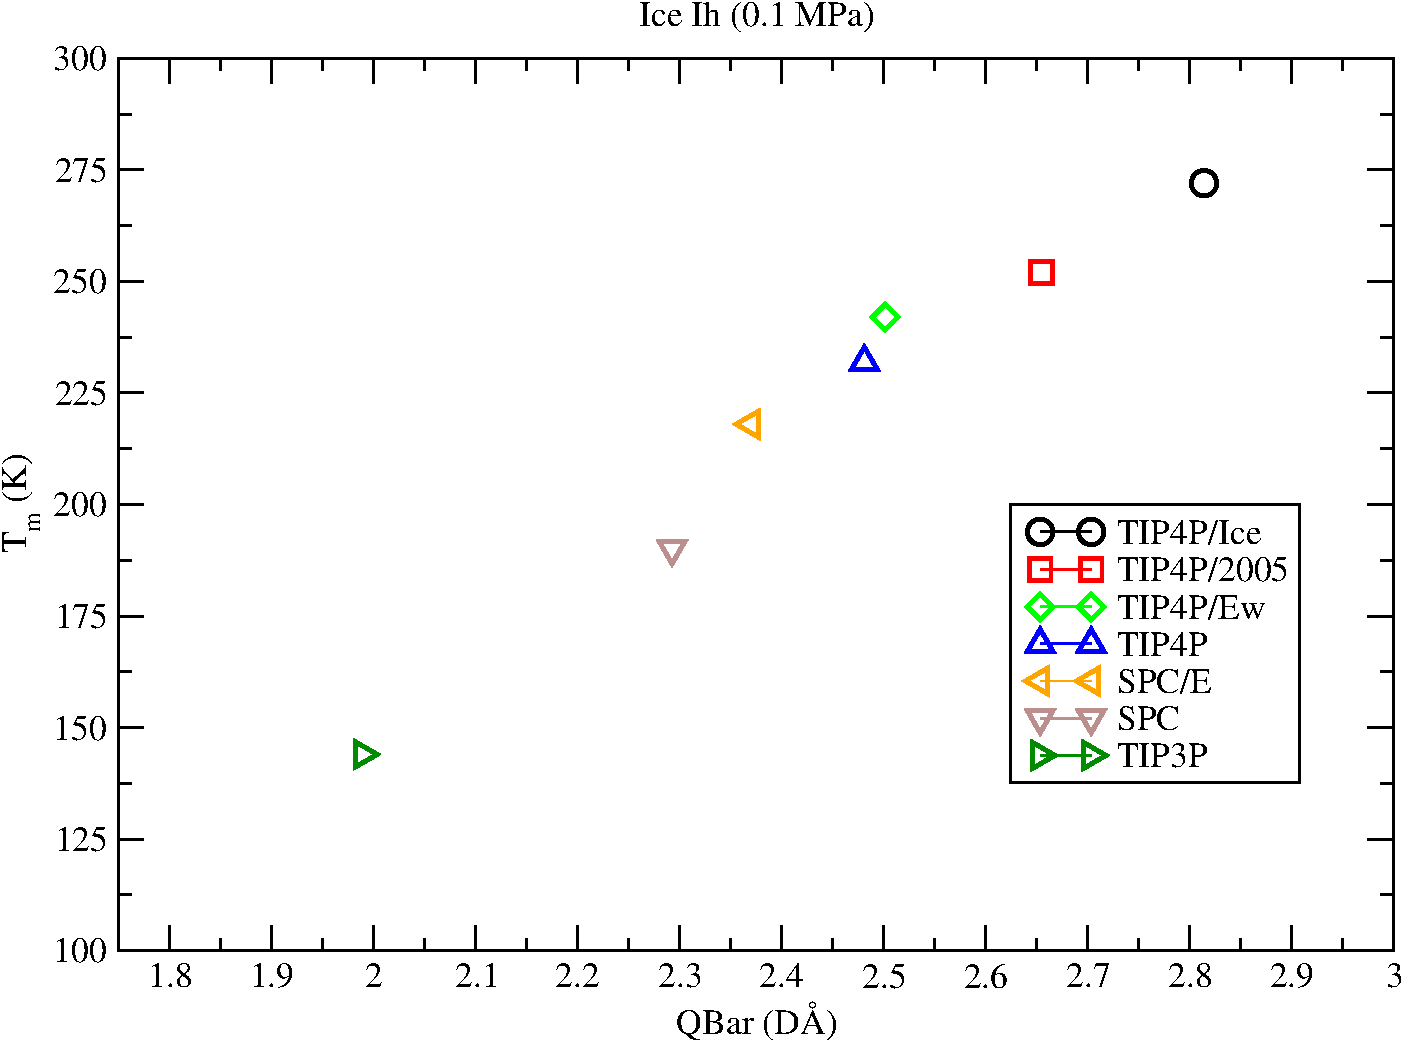
\includegraphics[width=\linewidth]{Figures/Tm_Ih_Qbar_plot.pdf}
\caption{\label{fig:QBar} Melting point for ice-I$_h$ of several
  popular water models as a function of the QBar for the model. We see
  a strong correlation between a more accurate melting point and a
  larger value of $\overline{Q}$. We estimate that a $\overline{Q}$ of
  approximately 2.8 D\AA~will result in the experimental melting point
  of 273.15 K. A linear regression of the data resulted in an equation
  of best fit of $y = 158.89x - 166.83$. From this, we have predicted
  an optimal $\overline{Q}$ to be 2.7690 D\AA~.}
\end{figure*}

\begin{figure*}
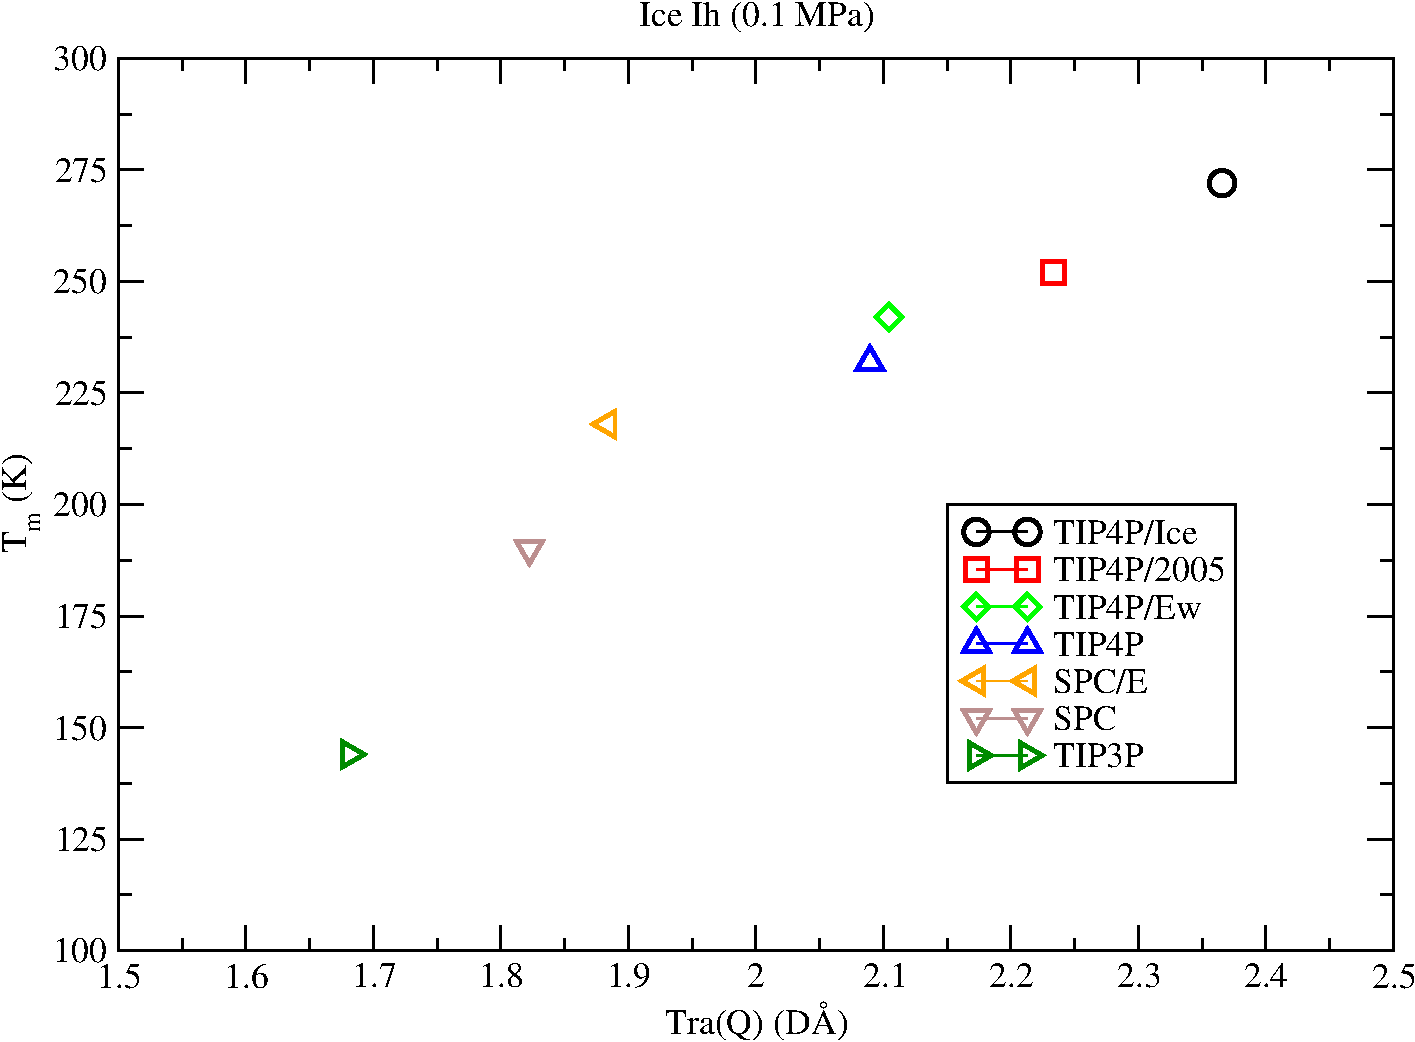
\includegraphics[width = \linewidth]{Figures/Tm_Ih_TraQ_plot.pdf}
\caption{\label{fig:TraQ} Melting point for ice-I$_h$ of several popular water models as a function of the trace of the quadrupole tensor for the model. We see a strong correlation between a more accurate melting point and a larger value of the trace. We estimate that a trace of approximately 2.3 D\AA will result in the experimental melting point of 273.15 K.}
\end{figure*}

While it is still unclear if these results are indicative of an
experimentally observable phenomenon, exploring correlations such as
this can help in the development of water models in the future. 


\subsection{Transport Properties}
Transport phenomena are processes that describe the transfer (flux) of
mass, heat, momentum, and charge by molecular motions. During this
process, the transferred quantity is conserved, \textit{i.e.}, the
moving quantity is neither created nor destroyed. Because of this, a set
of balance, or conservation equations can be written down describing
the movement of these quantities in the presence of a flux. The set of
balance equations for the transport of mass, energy and momentum are
presented in Table \ref{tab:transport}. 


\begin{table}
	\caption{BALANCE AND CONSTITUTIVE EQUATIONS FOR MASS, ENERGY, AND MOMENTUM TRANSPORT\label{tab:transport}}
        \begin{tabular}{rcc}
          \hline \hline
          & \textbf{~~Balance Equations~~} & \textbf{~~Constitutive Equations~~}\\ \hline 
          \textbf{~~Mass~~} & $\frac{\partial c (\vec{r}, t)}{\partial t} + \nabla \vec{j} = 0$ & $\vec{j} = -D \cdot \nabla c(\vec{r}, t)$\\
          \textbf{~~Energy~~} & $C_p \frac{\partial T (\vec{r}, t)}{\partial t} + \nabla \vec{J} = 0$ & $\vec{J} = -\lambda \cdot \nabla T(\vec{r}, t)$\\
          \textbf{~~Momentum~~} & $\rho \frac{D \vec{v}(\vec{r}, t)}{Dt}
                                  + \nabla \overleftrightarrow{\sigma} =
                                  0$ & $\sigma_{x,z} = -\eta \cdot
                                       \nabla_z (\rho v_x)$\\ \hline
          \hline
          \end{tabular}
\end{table}

When a transport flux is present, a characteristic response of the
material the flux is traveling through will become apparent. For
example, in the presence of an energy flux, a thermal gradient will
develop in the material. Likewise, a momentum flux will cause a
velocity distribution to form in the system. Through a series of
constitutive equations (right column of Table \ref{tab:transport}, it
is possible to relate the flux to the observed system response through
a proportionality constant describing the transport.  Following Fick's
Law, the diffusion coefficient, or diffusivity, ($D$) is the
proportionality constant describing the transport of mass, $\vec{j}$
and the resulting concentration gradient $\nabla c(\vec{r},
t)$. Similarly, by Fourier's Law, the thermal conductivity, $\lambda$,
is described by the energy flux $\vec{J}$ and the thermal gradient
through the material $\nabla T(\vec{r}, t)$. Lastly, from Newton's Law
of Viscosity, the shear stress( $\sigma_{x,z}$) and the velocity
gradient $\nabla_z (\rho v_x)$ are related through the shear viscosity
$\eta$. These constants are dependent on the material the transport is
occuring through, and thus are characteristic quantities of the
material.

% \begin{itemize}
% \item \textbf{Diffusion (Fick's Law):} $\vec{j} = -D \cdot \vec{\nabla}c(\vec{r},t)$ \vspace{0.05in}\\
% The diffusion constant, $D$, relates the mass flux to the concentration gradient.
% \item \textbf{Thermal Conductivity (Fourier's Law):} $\vec{q} = -\lambda \cdot \vec{\nabla} T(\vec{r},t)$ \vspace{0.05in}\\
% The thermal conductivity, $\lambda$, relates the heat flux to the temperature gradient.
% \item \textbf{Viscosity (Newton's Law of Viscosity):} $\sigma_{x,z} = -\eta \cdot \vec{\nabla}_z (\rho v_x)$ \vspace{0.05in}\\
% The shear viscosity, $\eta$, relates the shear stress to the velocity gradient $\left < d(v_x)/dz \right >$.
% \end{itemize}

\subsubsection{Green-Kubo Relations}
In the 1950s, Green and Kubo showed that transport coefficients
are directly related to the time dependence of equilibrium
fluctuations of the system. If we consider an arbitrary dynamic
property $A(t)$ with a total time derivative of $\dot{A}(t)$, then the
displacement at time $t$ is given by
\begin{equation}
A(t) - A(0) = \int_0^t dt' \dot{A}(t').
\end{equation}
Squarring both sides and averaging over time origins we obtain 
\begin{equation}
\langle [A(t) - A(0)]^2 \rangle = \int_0^t dt'' \int_0^t dt' \langle
\dot{A}(t') \dot{A}(t'') \rangle
\end{equation}
Recognizing that the integrand is symmetric in $t''$ and $t'$, and
that the integral is taken over a square in $t'-t''$ space, we can
integrate over one half the square and double the result. Further, if
we assume the property $\langle \dot{A}(t') \dot{A}(t'') \rangle$ to
be a stationary correlation function, then we are able to shift time
origins without issue. 
\begin{equation}\label{eq:gk}
  \langle [A(t) - A(0)]^2 \rangle = 2 \int_0^t dt'' \int_0^{t''} d\tau ~
  \langle \dot{A}(\tau ) \dot{A}(0) \rangle
\end{equation}
Equation \ref{eq:gk} is invariant under interchanging the two
integrations. Lastly, taking a long-time limit collapses one of the
integrals and we are left with a general relation describing the
mean-square displacement of a dynamic quantity and an integral of a
time correlation function.
\begin{equation}\label{eq:gk2}
 \gamma =  lim_{t \rightarrow \infty} \frac{\langle[ A(t) - A(0)]^2 \rangle}{2t} =
  \int_0^{\infty} d\tau ~ \langle \dot{A}(\tau ) \dot{A}(0) \rangle
\end{equation}
Solving for the transport coefficient ($\gamma$) of interest, is
simply a matter of determining the appropriate dynamic property
$A(t)$, and computing the long-time correlation function. However,
when implemented extracting transport coefficients from equilibrium
simulations in this manner is often computationally expensive. This is
due to the slow decay of the correlation function, resulting in the
need for long simulation times.

\subsubsection{Non-equilibrium Molecular Dynamics Methods}
An alternative approach to obtaining transport coefficients is through
the use of non-equilibrium molecualr dynamics (NEMD) simulations.
During NEMD simulations, the system is driven out of equilibrium by
the presence of an external perturbation (\textit{e.g.} a thermal or
velocity gradient), and the flux required to sustain the imposed
gradient is computed. Once in-hand, the computed flux and imposed
gradient can be used to obtain the transport coefficient through the
linear constitutive relations in Table \ref{tab:transport}.

For example, if the desired transport property is the thermal conductivity
($\lambda$) of a material, two regions of the simulation box will be
thermostatted, and the kinetic energy flux ($J$) required to maintain
the temperature difference will be calculated. Once this value is
converged, $\lambda$ can be obtained by
\begin{equation}\label{thermalTransport}
J_{z} = - \lambda \big(\frac{\partial T}{\partial z}\big)
\end{equation}
where the separation has been taken to be along the $z$-dimension of
the system.  Similarly, the shear viscosity ($\eta$) of a fluid can be
computed by determining the momentum flux ($ j_{z}(p_{x})$) required
to maintain a given average velocity in two spatially separated
regions. 
\begin{equation}\label{momentumTransport}
  j_{z}(p_{x}) = -\eta \big(\frac{\partial v_{x}}{\partial z}\big)
\end{equation}

Simulation times to converge the required flux to maintain the desired
thermal or velocity distribution are often shorter than when computing
transport properties using the Green-Kubo relations. However,
computing the appropriate flux can be quite challenging. Recently,
Kuang and Gezelter have developed an approach to non-equilibrium
molecular dynamics in which they invert the measured and imposed
quantites.\cite{Kuang2010,Kuang2012} In their method, aptly named
reverse non-equilibrium molecular dynamics, the flux is imposed across
two spatially separated regions of the simulation box, and the
gradient response is measured. Again, the desired transport
coefficient can be obtained through the linear constitutive
relations. This method is advantageous over NEMD approaches as the
gradient response of the system is often much easier to measure
compared to the difficult to compute flux.


%%%%%%%%%%%%%%%%%%%%%%%%
% Water is abundant and found everywhere.
% Water has a lot of weird properties.
% Because of this, ancient humans thought it was important.
% We shall start at understanding the structure of water in each
% phase, then consider coexistence.
%%%%%%%%%%%%%%%%%%%%%%%%
\section{H$_2$O: A Simple Molecule with Complex Behavior}
Water is the simplest compound that can be constructed from the two
most abundant reactive elements in the unvierse, oxygen and
hydrogen. It is also the second most common molecule in the universe,
trailing behind diatomic hydrogen, $\mathrm{H}_2$. It is composed of
two atoms of hydrogen and one atom of oxygen, and it has been found to
be fundamental to star formation.  On Earth, water occupies nearly
$1.4\times 10^{9}~\mathrm{km}^{3}$\cite{Brown2016}, and accounts for 40\% to
70\% of Earth's retention of heat. It is one of the few molecules that
can be found in its solid, liquid, and gasseous forms at ambient
temperatures and pressures.  Some hypothesize that life cannot exist
without water, as all forms of life found thus far depend on
it.\cite{Caldecott2008,Henry2005} In many organisms, water comprises
XX percent of their chemical makeup, with as large as XX in others. In
humans, water composes nearly half the volume of each
cell.\cite{Ling2004} It is the ubiquitus nature of water and ice that
gives rise to its importance; due to its natural abundance a wide
variety of chemistry and physical processes occur within this medium,
and at its surfaces.

Besides being found everywhere in naturally occurring abundance, water
expresses numerous structural, dynamic, and thermodynamic
anamolies.\cite{Brovchenko2008}. The melting, boiling, and critical
points are unusually high for similar size molecules. The denisty of
ice increases upon heating (up to 70~K). The density of the liquid
increases with increasing temperature (up to $\sim$ 281 K). Pressure
can melt the solid rather than freezing the liquid, and there are more
solid phases than observed for similar sized molecules. While the
principles governing these and many other unique properties of water
are not known, many of the observed anomolies are attributed to the
electronic distribution around water and the resulting strength of the
hydrogen bond.

In ancient times, humans recognized the importance of water. The Greek
philosopher Thales of Miletus, one of the seven sages of antiquity,
declared that everything was composed of water (around 700 BCE). Later
in the 5th century BCE, Empedocles described water as being one of
four 'classical' elements of the ancient world, alongside earth, wind,
and fire. Likewise, the ancient Chinese described the world around them
using five elements, earth, wood, metal, fire, and water. The
importance of water was discovered early in our human history, and it
has been studied extensively since those early days.

\subsection{The Structure of Water}
%
% description of what water is? structure constitution etc?
% Gas phase molecule in isolation
% Condensed phase liquid water as collection
% Description of ice and it's structures
%
Defining water's structure can prove a bit challenging. This is mainly
due to the vast number of observed structures and configurations it is
found in. In the liquid, the dynamic hydrogen bond network evolves
rapidly; hydrogen atoms diffuse much more quickly than their
counterpart oxygen atoms due to `bucket-brigade' like motion. In the
solid phase, motion occurs much slower. However, motion is observed
around crystalline defects. There is also a large diversity in the
crystalline structures of water ice, as over sixteen unique crystal
structures have been observed or predicted\cite{Chaplin2018}, many of
which can be seen in Figure \ref{fig:phaseDiagram}

\begin{figure*}
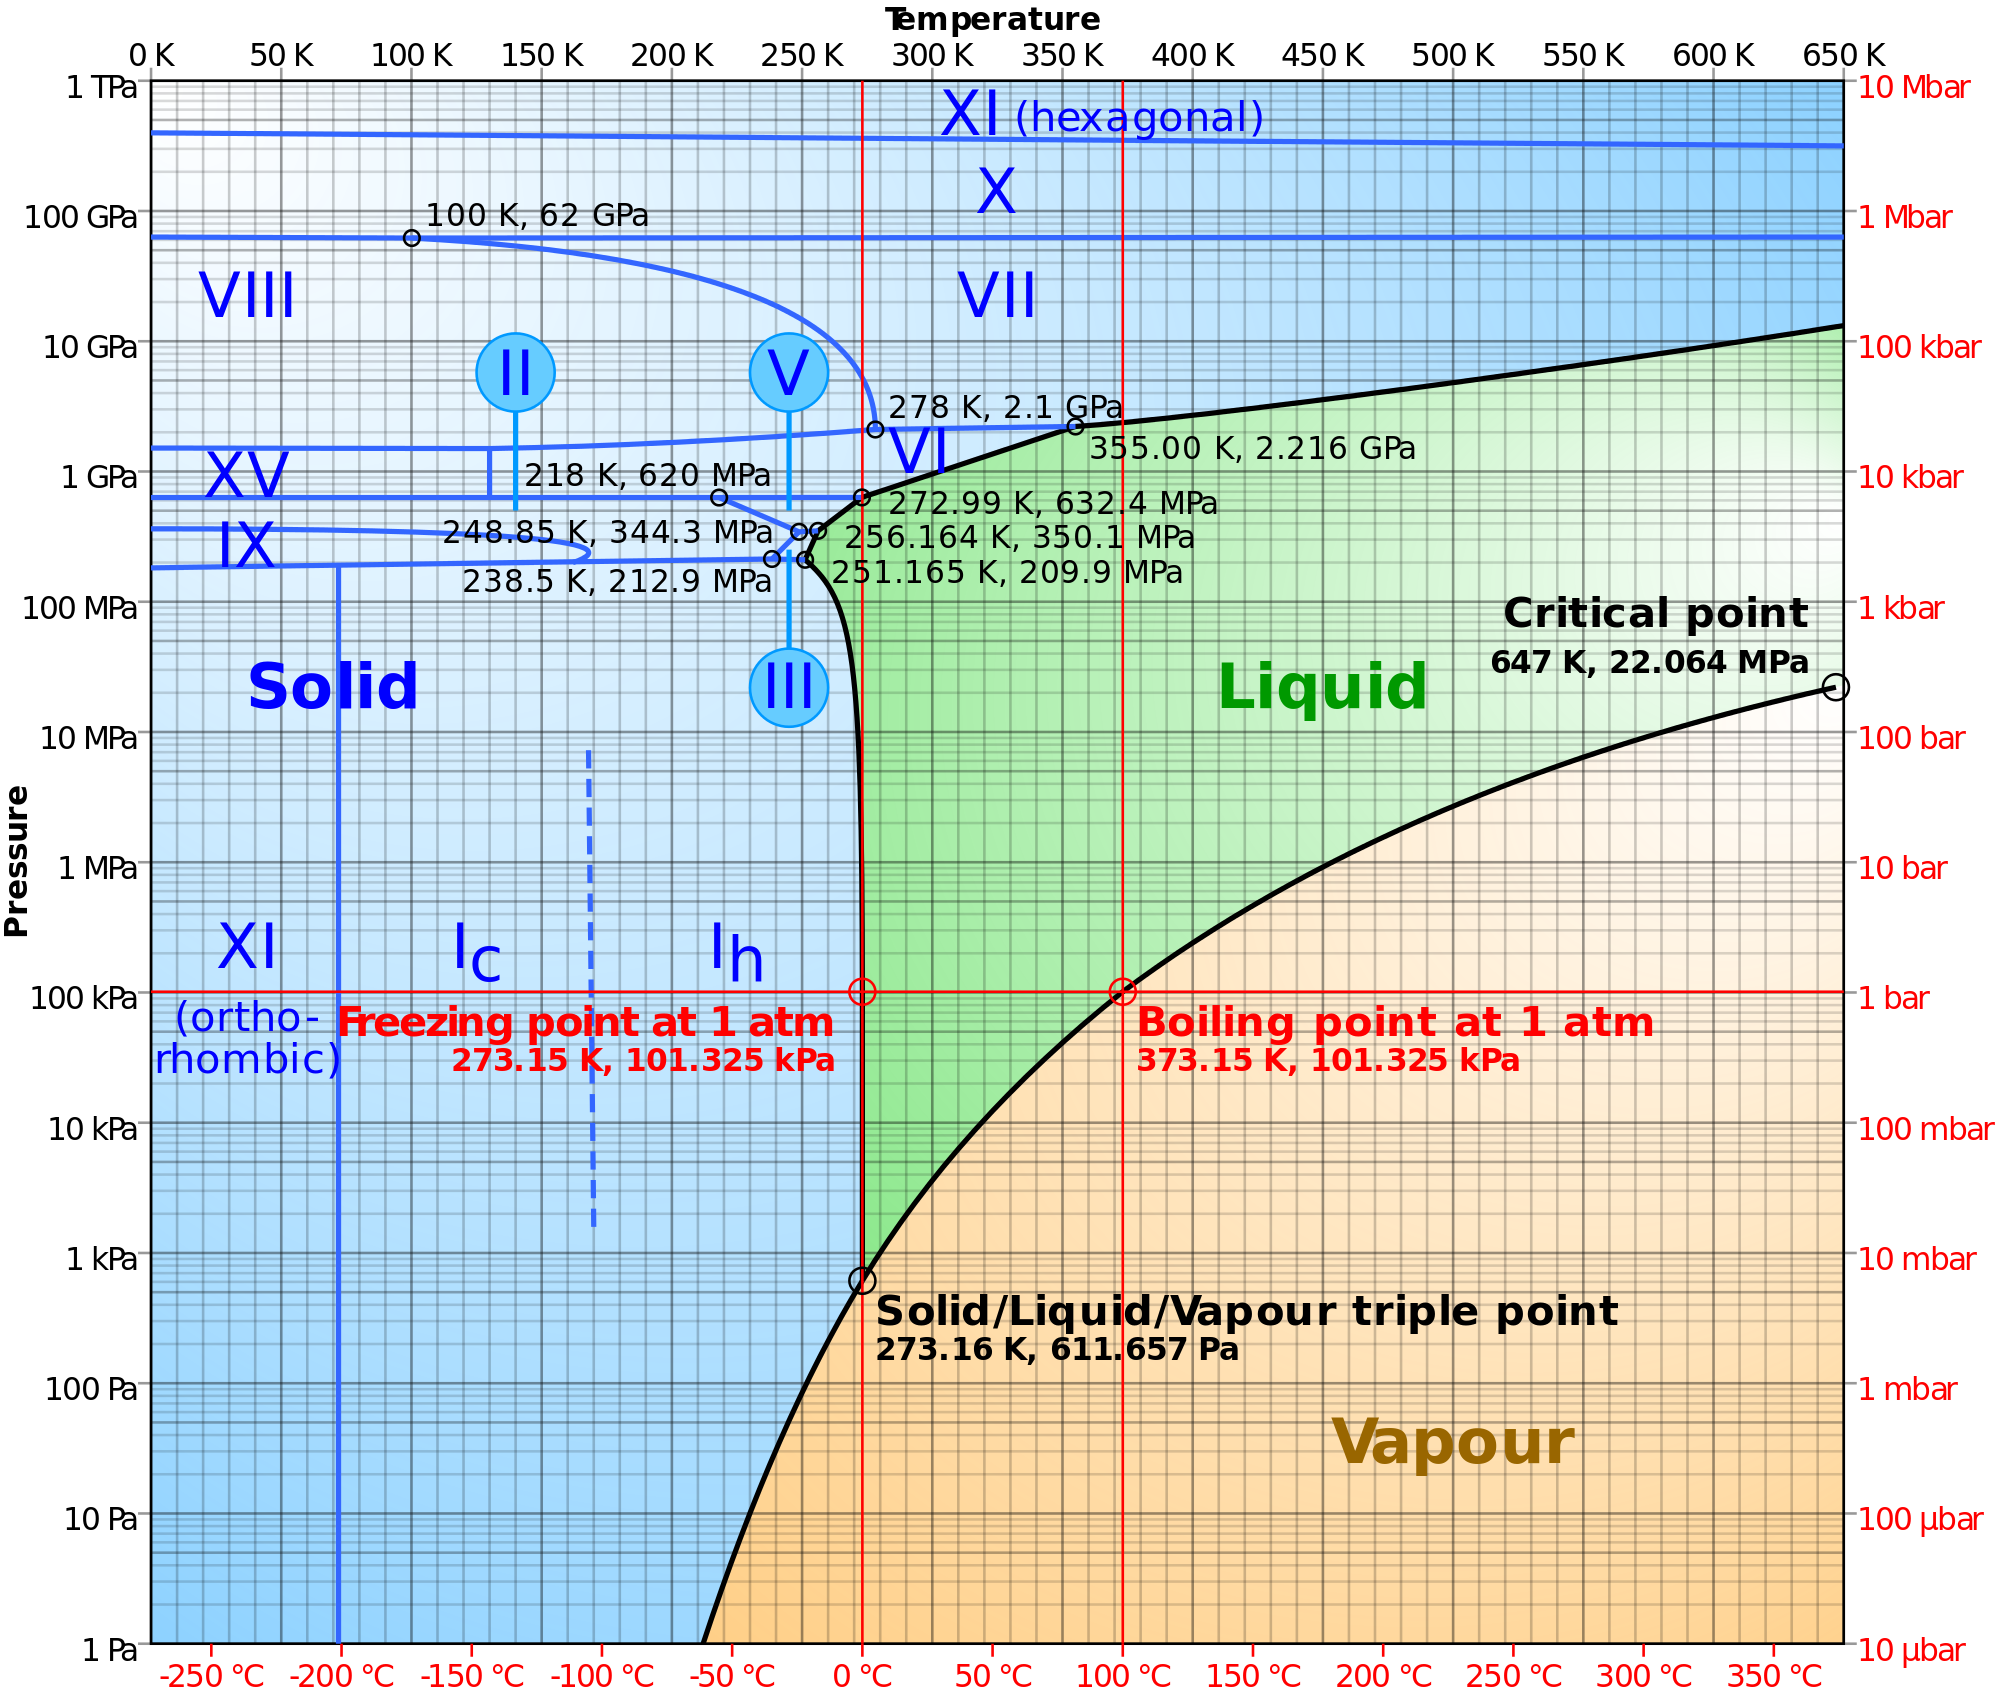
\includegraphics[width=\linewidth]{Figures/PhaseDiagram}
\caption{\label{fig:phaseDiagram} The phase diagram of
  water.\cite{Zhang2015} dT$_{C}$ / dP $<$ 0 at the following boundaries:
  ice-II to ice-V, liquid to ice-I$_\mathrm{h}$, and ice-VII to
  ice-VIII. Conversely, dT$_{C}$ / dP $>$ 0 at the following boundaries:
  liquid to vapour, liquid to ice-(V, VI, VII). dT$_{C}$ / dP $\approx$
  $\inf$ at the ice-(VII, VIII) to ice-X boundary occurring at 60 GPa.
  dT$_{C}$ / dP $\approx$ 0 at ice-I$_\mathrm{h}$ to ice-XI boundary at
  low temperatures. }
\end{figure*}


\subsubsection{Gaseous Water}
In the gas phase, water adopts a `bent-like' geometry, with an HOH
bond angle of about 104.5\degree~. The oxygen-hydrogen bond length as
computed by high accuracy quantum mechanical calculations gives 1
\AA~. These bond lengths and bend angles are an equilibrium value, as
they are constantly vibrating. Even at $-$273.15~\degree C some
residual vibrations remain. This is described as a zero-point energy,
and has considerable implications for the potential energy of the
molecule.

Water's electrons are not symmetrically distributed about the
molecule. This gives rise to higher order multipoles, and it is these
electronic distributions that give rise to many of water's
characteristic properties. In the gas phase, water has a dipole moment
of about 1.85~D. This dipole moment is highly polarizable, that is, it
readily responds to an external electric field, be it applied or
created by molecules in its local environment. In the condensed liquid
phase, the dipole moment becomes much harder to probe, but values have
been reported ranging from 2.2~D to 2.9~D.


\subsubsection{Liquid Water}
Water is a liquid at room temperature because of its large dipole
moment and the strength of the intermolecular hydrogen bonds. These
bonds are significantly stronger than the van der Waals interactions
arising from the instantaneous polarization of molecules. Numerically,
hydrogen bonds have a strength of about 20
$\mathrm{J}~\mathrm{mol}^{-1}$, about ten times thermal fluctuation at
room temperature. The order of magnitude difference between the
intermolecular interactions and thermal fluctuations means that the
liquid will not boil at room temperatures. The intermolecular forces
for similar size molecules are weaker, for example
$\mathrm{H}_2\mathrm{S}$ boils at -60~\degree~C. The strong hydrogen
bonds and the large dipole moment of water holds the molecules
together in a condensed phase at room temperature.

The polarizability of a water molecule leads to another interesting
property, namely, its local bonding environment. In the liquid phase,
water molecules often adapty tetrahedral like geometries with other
water molecules, resulting in $\sim$~3 nearest neighbors at ambient
conditions. The maximum density of the liquid is observed to occur at
$\sim$~4\degree~C, and cooling further results in decreasing
density. Liquid water transitions to ice when the local ordering
becomes long ranged.


\subsubsection{Water Ice}
%
% Describe crystal structures of ice, examples of where some occur.
% Proton disordered structure, residule entropy. 
%
%Annu. Rev. Phys. Chem. 2017. 68:285–304
Water ice is a fundamental solid, with implications in biological,
environmental, geological, and extraterrestial
phenomena.\cite{Shultz2017} Biologically, many organisms have had to
adapt to advancing ice fronts. These organisms produce antifreeze
proteins which disrupt the hydrogen bonding network at the ice /
liquid interface, preventing further ice growth. The movement of
glaciers has carved out surface features on Earth, and throughout our
solar system reactions and transport of a wide variety of molecules
occurs at the surface of ice.


% John Finney, A Very Short Introduction to Water. Oxford University
% Press. 
The structure of hexagonal ice (ice-I$_\mathrm{h}$) has been studied
extensively using experimental methods such as neutron scattering and
x-ray spectroscopy, as well as NMR and laser
spectroscopy.\cite{w. F. Kuhs and M. S. Lehmann, in Water Science
  Reviews 2, edited by F. Franks (Cambridge University, New York,
  1986),pp. 1-65.}  In this structure, water molecules form puckered
six member rings, with OOO angles formed by three neighboring
molecules close to 109.5\degree~. These rings can stack on top of one
another and expand to form large sheets, giving rise to the observed
six-fold symmetry of snowflakes. Due to the open structure of the
crystal, it is possible to interweave an equivalent second ice crystal
through the first. These structures have a larger density than the
more open ice, and are aptly named ultra-high density ices. Ice also
crystallizes into cubic structures, although no interwoven lattice has
yet been observed for this geometry. In total, there are currently 16
different crystal structures known for water ice, some of which can be
seen in Figure \ref{fig:phaseDiagram} and Table \ref{tab:iceProps}. 

\begin{table}
\centering
\caption{ICE CRYSTAL SYMMETRY AND HYDROGEN ORDERING}
\label{tab:iceProps}
\begin{tabular}{lccc}  
\hline\hline 
  ice form & crystal structure & density (g cm$^{-3}$) & proton arrangement  \\ \hline
  I$_\mathrm{h}$ & hexagonal & 0.92 & disordered \\
  I$_\mathrm{c}$ & cubic & 0.93 & disordered \\
  II & rhombohedral & 1.17 & ordered \\
  III & tetragonal & 1.14 & disordered \\
  IV & rhombohedral & 1.27 & disordered \\
  V & monoclinic & 1.23 & disordered \\
  VI & tetragonal & 1.31 & disordered \\
  VII & cubic & 1.50 & disordered \\
  VIII & tetragonal & 1.46 & ordered \\
  IX & tetragonal & 1.16 & ordered \\
  X & cubic & 2.51 & symmetric \\
  XI & orthorhombic & 0.92 & ordered \\
  XII & tetragonal & 1.29 & disordered \\
  XIII & monoclinic & 1.23 & ordered \\
  XIV & orthorhombic & 1.29 & ordered \\
  XV & pseudoorthorhombic & 1.30 & ordered \\
  XVI & cubic & 0.81 & disordered \\ 
\hline \hline
\end{tabular}
\begin{flushleft}
Data taken from Reference \cite{Chaplin2018}.
\end{flushleft}
\end{table}

% Ice Ih at -30 \degree ~C, apply 30,000 atmospheres of pressure
% and we will observe a phase transition to ice-III. Similarly, cool
% ice-III to -40 degrees Celcius and we will see a phase transition to
% ice-II. There are approximately sixteen different known crystal
% structures of ice, each one stable in some unique region of the phase
% diagram. Also, there are ice phases which have been predicted by
% computer simulation which have not yet been observed in vivo. If we
% inspect the phase transition from ice-Ih to ice-III closer, we will
% see a distortion in the crystalline geometry under the large pressure
% conditions. Some of the puckered six-membered rings will compress into
% five-membered structures, resulting in a more dense packing of water
% molecules. However, this will place more strain on the
% hydrogen-bonds. In ice-III, the OOO bond angles vary between 88
% degrees and 148 degrees. Likewise, the hydrogen-bond lengths will also
% change under this distortion. In ice-Ih, hydrogen-bonds are typically
% 0.276 nm, in ice-III hydrogen-bonds are found between 0.271 nm and
% 0.283 nm.

In 1933, Bernal and Fowler established a set of rules for populating
hydrogens into an oxygen ice lattice. These rules are as follows;
each oxygen atom is covalently bonded to two hydrogens, and each
hydrogen in each water molecule forms a hydrogen bond with one other
oxygen. This means there is exactly one hydrogen between every two
oxygen sites in the lattice. The result of these rules is that each
oxygen is in a tetrahedral environment, and is donating two hydrogens
and accepting two hydrogen bonds.

Following these ice-rules, we see that there are two \textit{kinds} of
crystals that can be obtained, \textit{ordered} and
\textit{disordered}. In the \textit{ordered} case, the hydrogen
configurations for equivalent water molecules in all unit cells are
the same, whereas in a \textit{disordered} ice the proton
configurations are unequivalent. We can describe these lattices as
being orientationally ordered or disordered, however, they are more
commonly described in terms of their proton ordering. The two
descriptions are equivalent as the arrangement or ordering of the
hydrogens gives rise to the orientation of the water molecules.  Ice-
I$_\mathrm{h}$, III, IV, V, VI, VII, XII, XVI are proton disordered,
while ices II, VIII, IX, and XI are proton ordered.

Upon cooling, ice-III and ice-VII undergo a phase transition to
ordered forms, ice-IX and ice-VIII respectively. Transitions of proton
disordered ice to proton ordered ice must inherently involve the
reorientation of water molecules, the transfer of hydrogens, or some
combination of the two. However, if all molecules in the lattice
satisfy the Bernal Fowler ice-rules, any one water molecule
reorientation or proton transfer will inevitably break the
ice-rules. Therefore, we conclude these events must happen in concert,
large collections of molecules must simultaneously undergo some
combination or reorientation and proton transfer. However, the energy
required to do so would be quite large, and larger still for
increasing number of molecules involved. This amount of energy is not
likely available at the thermal conditions where these transitions are
observed to occur, therefore, it is believed that the these
transitions must depend on defects within the lattice. 

There are two known kinds of defects in ice
lattices, \textit{orientational} defects, known as Bjerrum defects,
and \textit{ionic} defects. There are two kinds of Bjerrum defects,
D-defect (from the German \textit{doppelbesetze} meaning doubly
occupied), and an L-defect (from \textit{leere} meaning empty). A
D-defect occurs when there are two hydrogens between two neighboring
oxygens, and an L-defect occurs when there are no hydrogens between
the oxygen sites. These are of course in violation of the Bernal
Fowler ice-rules, however, they act as proton sinks and sources when
the crystal undergoes phase transitions from proton disordered to
proton ordered. Ionic defects form when a proton transfer happens
between two oxygens, resulting in the formation of a hydroxide and
hydronium ion.

% Residual Entropy of ice.
If we further consider the Bernal Fowler ice-rules, we see that the
hydrogen arrangement in ice-I$_\mathrm{h}$ is not unique. In 1935,
Linus Pauling argued that any arrangements of hydrogens which
satisfies the ice-rules is valid and has equal probability of
occuring since each unique arrangement has the same energy,
\textit{i.e.} they are degenerate configurations. Due to this, he
predicted ice-I$_\mathrm{h}$ to have a \textit{residual entropy}, that is, a
non-vanishing positive entropy ($S_{0}$) at zero Kelvin. This entropy
can be computed from Boltmann's equation of statistical mechanics,
\begin{equation}\label{eq:Boltzmann-W}
S = k_{B}~\mathrm{ln}(W)
\end{equation}
where $k_{B}$ is Boltzmann's constant and $W$ is the number of
equivalent arrangements of the molecules. Pauling estimated the number
of configurations in two separate ways.\cite{Pauling1935} First, we
consider that there are possible six ways to orient a water molecule
within a tetrahedral structure formed by neighboring molecules while
satisfying the ice-rules. If we give each water molecule one of these
six orientations at random, there is then a 1/2 probability of having
a hydrogen between two oxygens, thus there is a 1/4 chance that there
is exactly one hydrogen between every two oxygens in the lattice. The
resulting number of correct possible arrangements of $N$ water
molecules is
\begin{equation} \label{eq:Pauling-1}
W_{Pauling} = (6/4)^{N} = (3/2)^{N}.
\end{equation}   
Pauling arrived at the same result by a second construction. If we
 only enforce there to be a single hydrogen
between each oxygen in the lattice, there are $2^{2N}$ configurations
(since there are $2N$ bonds in the network). For each oxygen atom,
here are $2^{4} = 16$ possible arrangements for the hydrogens, 10 of
which are ruled out as they result in non-intact
molecules. That is, they form structures of (H$_{4}$O)$^{2+}$,
(H$_{3}$O)$^{+}$, (HO)$^{-}$, and O$^{2-}$. Therefore, there are only
6/16 possible configurations allowed for placing hydrogens around each
oxygen. This gives a total number of configurations as,
\begin{equation}
W_{Pauling} = 2^{2N}(6/16)^{N} = (3/2)^{N}.
\end{equation}
Using these results with Equation \eqref{eq:Boltzmann-W}, the residual
entropy follows as
\begin{equation}
S_{0} = k_{B}N\mathrm{ln}(3/2) = R\mathrm{ln}(3/2)
\end{equation}
where $R$ is the molar gas constant,
$R = 8.31447~\mathrm{J~mol}^{-1}~\mathrm{K}^{-1}$. This gives a
residual entropy of
\begin{equation}
  S_{0} = 3.3712~\mathrm{J~mol}^{-1}~\mathrm{K}^{-1} = 0.80574~\mathrm{cal~deg}^{-1}~ \mathrm{mol}^{-1}.
\end{equation}
The residual entropy has been further investigated by Berg \textit{et
  al.} who obtained
$S_{0} \approx 0.81550 \pm 0.00021~\mathrm{cal~deg}^{-1}
~\mathrm{mol}^{-1}$ by means of multicanonical
simulations.\cite{Berg2007} This result was found to be in good
agreement with a series expansion method by Nagle \textit{et
  al.}\cite{Nagle1966}, as well as Giaque and Stouts calorimetry
experiments which estimated
$S_{0} = 0.82 \pm 0.05~\mathrm{cal~deg}^{-1}
~\mathrm{mol}^{-1}$.\cite{Giaque1936}
% end Residual Entropy of ice.



\subsection{Hydrogen Order at the Surface of Ice}
It is well understood that the formation of a surface requires
considerable energy, although, the molecules at the surface have
interesting characteristics unique to their local
environment. Termination of the repeating crystal lattice results in
undercoordinated molecules which have enhanced mobility at appreciable
temperatures due to the reduced potential experienced at these
sites.\cite{} Similarly, surface platinum atoms have been observed to
be catallytically active due to their coordination.\cite{}

For most materials, crystal surfaces are often defined by the surface
plane relative to the internal coordinates. Ice-I$_\mathrm{h}$
crystals commonly expose the $\{0001\}$ (basal) and $\{10\bar{1}0\}$
(prismatic) faces, although, this does not completely define the
surface as compared with simple solids. Due to the residual entropy of
the proton distribution within the ice lattice, termination of the
crystal along the desired plane but at varying locations throughout
the crystal can result in differential hydrogen patterning at the
surface. The possible proton arrangements could alter the surface
energy ($\gamma$), a thermodynamic quantity that affects crystal growth and
controls crystal shape.

Fletcher was the first to consider proton ordering at
ice-I$_\mathrm{h}$ surfaces, using classical electrostatics arguements
to suggest that the lowest energy surface should be proton
ordered.\cite{Fletcher1992} His arguements stemmed from dipole
interactions among nearest neighbor OH bonds, which also led to the
prediction that the basal surface would undergo a proton ordered to
disordered transition at $\sim$~30~K, and $\sim$~70~K for the
prismatic surface. 

More recently, Buch \textit{et al.} compared basal surfaces with
varying proton arrangements using the TIP4P/Ice and EMP water
models.\cite{Buch2008} They also found that proton ordered surfaces
were of lower energy as compared to disordered states, and observed
alternating rows of proton-exposed and oxygen-exposed termination to
be the most stable.  Pan \textit{et al.} performed density-functional
theory (DFT) calculations on the basal and prismatic surface of an
ice-I$_\mathrm{h}$ and obtained similar surface energies for the two
faces.\cite{Pan2010} However, they observed a strong dependence for
the surface energy on the proton ordering, which was found to account
for up to 50~\% of the total surface energy (significantly larger than
proton ordering in the bulk $<$ 1~\%). This suggests that the ice
surface's thermodynamic ground state will be proton ordered, even for
temperatures well above the bulk order-disorder temperature of about
72~K.

The surface energies for an antiferroelectric ice, ice-XI, were found
to converge with variying exchange-correlation functionals on a value
of about $\gamma_{basal}^{XI} \sim 11~\mathrm{meV~\AA^{-2}}$. However,
the surface energies for ice-I$_\mathrm{h}$ were observed to be spread
over a much larger range of values, from 12.2 to 18.2~
$\mathrm{meV~\AA^{-2}}$. This indicates that for a constant internal
ice-I$_\mathrm{h}$ lattice, slight changes in proton ordering at the
surface can result in large differences in surface energy.

Lastly, Pan \textit{et al.} investigated the surface oxygen
positions. With a reduction in their experienced potential, these
oxygen atoms could deviate from their lattice positions with thermal
energy. For the ice-I$_\mathrm{h}$ surface bilayers, they find the
oxygen - oxygen distance does not change much compared to the
bulk. The average surface oxygen - oxygen distance is 0.02 \AA~
greater than found in the bulk. This is consistent with experimental
results, indicating distances of 2.77 \AA~ for surface and 2.76 \AA~
for bulk at 38~K.\cite{Parent2002} 

\subsection{Ice / Water Coexistence}
%%%
% General introduction to ice/water coexistence
% Early work in the field, quiescent systems and measures of
% interfacial width.
% Problems discovered specific to ice/water coexistence, improper
% treatment of the electrostatics, coexistence temperatures, etc.
%
%%%

%%%
% from iceWater.tex
%
%
%%%

Understanding the ice / water interface is essential for explaining
complex processes such as nucleation and crystal
growth,\cite{Han1992,Granasy1995,Vanfleet1995} crystal
melting,\cite{Weber1983,Han1992,Sakai1996,Sakai1996B} and some
fascinating biological processes, such as the behavior of the
antifreeze proteins found in winter flounder,\cite{Chapsky1997
  ,Wierzbicki2007} and certain terrestrial
arthropods.\cite{Duman:2001qy,Meister29012013} Haymet \textit{et al.}
have done extensive work on ice-I$_\mathrm{h}$, including
characterizing and determining the width of the ice/water interface
for the SPC,\cite{Karim1990} SPC/E,\cite{Gay2002,Bryk2002}
CF1,\cite{Hayward2001,Hayward2002} and TIP4P~\cite{Karim1988} models
for water.  More recently, Haymet \emph{et al.} have investigated the
effects cations and anions have on crystal
nucleation.\cite{Bryk2004,Smith2005,Wilson2008,Wilson2010} Nada
\textit{et al.}  have also studied ice/water
interfaces,\cite{Nada1995,Nada2000,Nada2003,Nada2012} and have found
that the differential growth rates of the facets of ice-I$_\mathrm{h}$
are due to the the reordering of the hydrogen bonding network at the
interface.\cite{Nada2005}


% Benet, MacDowell, Sanz, PCCP 2014, 16, 22159
% A study of the ice/water interface using the TIP4P/2005 water model

The interfacial free energy between ice and
water, $\gamma_{iw}$, is a crucial parameter for ice nucleation and
crystal growth.\cite{1,2} Experimentally obtained values of
$\gamma_{iw}$ range from 25 to 35
$\mathrm{mN}~\mathrm{m}^{-1}$.\cite{1} This spread stems from the
problem that there are no current methods for obtaining a robust
measurement. Computer simulations have attempted to quantify
$\gamma_{iw}$, and predictions have been made for a series of water
models, some with\cite{4} and some without\cite{5} taking full
electrostatic interactions into account. These studies used a varient
of the cleaving method,\cite{6} and estimated $\gamma_{iw}$ using the
TIP4P, TIP4P-Ew, and TIP5P-E water models.

Previously, $\gamma_{iw}$ has been estimated using the TIP4P/2005
water model and the method pruposed by Bai and Li, studying the
crystal-melt interface of a Lennard-Jones system.\cite{10} In the
method of Bai and Li, the critical size of crystalline clusters are
measured, and by extension of classical nucleation theory
$\gamma_{iw}$ can be obtained.\cite{11,12} This result produces an
orientationally averaged estimate of $\gamma_{iw}$, which does not
provide any information on the dependency of $\gamma_{iw}$ on the
orienation of the crystal.

Benet \textit{et al.} have measured the interfacial free energy of
ice-I$_\mathrm{h}$ in coexistence with liquid water at 248.5~K by
using the TIP4P/2005 water model by analysing the spectrum of
capillary fluctuations at the interface.\cite{Benet2014} This method
was originally described by Hoyt \textit{et al.}\cite{Hoyt2001}, has
been used to calculate the interfacial free energy of hard
spheres,\cite{14} the Lennard-Jones potential,\cite{15} and dipolar
fluids.\cite{16}

% In this method, water molecules were labeled as ice-like or
% liquid-like based on local bond order parameters. Next, a discretized
% profile parrallel to the interface (i.e, along the $x$ dimension),
% $h(x_{n})$, was computed for many small bins across the system. These
% resulting profiles were then Fourier-transformed,
% \begin{equation}
% h_{q} = \frac{1}{N}\sum_{n=1}^{N} h(x_{n})e^{iqx_n}
% \end{equation}
% giving an amplitude $h_{q}$ for each wave vector $q$, for each of the
% $N$ total bins across the $x$-dimension. 

% Capillary wave theory provides a relationship between these wave
% vector amplitudes and the interfacial stiffness, $\sigma$ by
% \begin{equation}
% \langle |h_{q}|^{2} \rangle = \frac{k_{B}T}{A \sigma q^{2}}
% \end{equation}
% where $A$ is taken to be the product of the two simulation box
% dimensions not normal to the interface. Since the interfacial
% stiffness is dependent on both the crystal plane that is exposed to
% the liquid and the direction which the wave vector propogates, we have
% \begin{equation}
% \sigma = \bigg(\gamma (\theta ) + \frac{d^{2}\gamma (\theta )}{d\theta
% ^{2}} \bigg)_{\theta = 0} .
% \end{equation}
% Here, $\theta$ is the angle between the average planar ice / water
% interface, and the normal vector of the instantaneous interface. The
% orientational dependence of the interfacial free energy can be written
% as an expansion of the Spherical Harmonics\cite{23}, and will be
% unique for each crystal plane studied. 

Benet found an orientationally averaged interfacial free energy of
$27 \mathrm{mN}~\mathrm{m}^{-1}$, which agrees well with recent
estimates using size cluster analysis by Sanz \textit{et
  al.}\cite{Sanz2013}. Benet \textit{et al.} were able to estimate the
free energy of different planes (in coexistence with liquid), and
obtained values of 27 $\pm$ 2, 28 $\pm$ 2, and 28 $\pm$ 2
$\mathrm{mN}~\mathrm{m}^{-1}$ for the basal, prismatic, and a higher
order surface face, the secondary prismatic surfaces,
respectively. They also observed an interfacial thickness of about
four to five molecular diameters, which was found to be insensitive
to the crystal face exposed to the liquid. Lastly, when the basal face
is exposed to the liquid, they observed local areas of hexagonal ice
and cubic ice within the interface. This observation is not unique to
this study, other simulations and experiments have shown hexgonal ice
to grow with a mixed Ic-Ih stacking.\cite{43-47}
%end Benet, MacDowell, Sanz, PCCP 2014, 16, 22159



\subsection{The Surface Premelting of Ice and the Quasi-Liquid Layer}
% 2. Driving force for the QLL, not unique to ice. Interesting on ice
% because ice occurs everywhere in the universe, therefore, lots of
% interesting things happen at ice surfaces.
% 3. Experimental and theoretical measures of the QLL, who and how have
% studied it.
% 3a. QLL width
% 3b. QLL structure, dynamics
% 4. Observed oddity of friction on ice surfaces is small, transition to
% next subsection where we will talk about friction studies on ice surfaces.


In order to understand the surface premelting of ice, we must first
understand what this surface looks like. A wide variety of
experimental techniques have been used to determine the structure,
dynamics, properties, and width of this liquid-like surface film.
Materer \textit{et al.} studied an ultrathin ice surface exposing the
basal face grown on a Pt(11) substrate at 90K (well below complete
surface melt) using low-energy electron diffraction (LEED)
spectrocopy, in conjunction with total-energy calculations and
molecular dynamics simulations.\cite{Materer1995,Materer1997} Their results suggested
the basal face is terminated with a full bilayer of molecules, and not
a half bilayer as some had previously conjectured. The same surface
structure was observed later by NAME using helium atom scattering
experiments at 30K.\cite{Braun1998,Glebov2000}

Sum frequency generation (SFG) spectroscopy is able to probe the
orientational disorder of molecules at a surface. The basal surface of
ice-I$_\mathrm{h}$ is known to present dangling or 'free' O-H bonds
normal to the interface. The orientational order of these dangling
bonds can be probed using SFG spectroscopy, and observing the
temperature at which the intensity of the SFG signal decreases can
estimate the onset of the QLL. Name and Name have probed the basal
surface using this technique for temperatures betwen 173-271
K~.\cite{Wei2001,Wei2002} They observed that the disorder became apparent
as the temperature approaches 200 K~, and increased with warmer
temperatures.  These results indicate that the structural ordering
decreases in a continuous fashion from bulk ice to the liquid-like
layer, which also agree with results from proton channeling and
glancing-angle X-ray scattering.\cite{Golecki1978,Dosch1995} Using
molecular dynamics simulations, Ikeda-Fukazawa and Kawamura found
molecules present on the surface of a basal plane with large
vibrational and rotational motions at temperatures well below the bulk
melting temperature.\cite{Ikeda-Fukazawa2004} Their results supported
the continous variation of structural ordering across the qausi-liquid
layer observed by the SFG spectroscopy.



% Ice Surfaces by Mary Jane Shultz, Ann Rev Phys Chem
(on qll) 'techniques as diverse as glancing angle X-ray (102, 103),
SFG (82), He atom scattering (104), atomic force microscopy (105,
106), ellipsometry (107), photoelectron spectroscopy (108), nuclear
magnetic resonance (NMR) (109, 110), theory (111–114), and
differential interference contrast (57, 115, 116) conclude that the
QLL exists.' The onset temperature has varied from as cold as 200K to
as warm as 260K, and discrepencies have been attributed to
contaminations to varying probe depths. There is also considerable
disagreement about the nature of the QLL, 'Theory indicates that it is
ordinary supercooled water (117), whereas recent interfacial force
microscopy (105) suggests that the QLL is neither ice nor water but
rather a new viscoelastic phase.' And recently Suzuki \textit{et al.}
have probed the QLL and observed two separate immesible liquid water
flims. 


Section 4.1 deserves further reading, talks about thermodynamics of
the basal, prism, and secondary prismatic crystal surfaces.
%end Annu. Rev. Phys. Chem. 2017. 68:285–304

% /Ice Surfaces.


For ice-I$_\mathrm{h}$, the temperature at which surface molecule
vibrations become prevelent at has been reported between 200K and
271K. Experimentally the surface molecules have been probed using a
variety of techniques and have determined slightly different
temperatures at which these internal vibrations become prevelent.

Both experiment and theory agree that the thickness of the QLL on ice
increases approaching T$_\mathrm{m}$, and values have been reported
between 2 nm to over 45 nm at 271~K. Part of the reason for the
discrepency is due to the definition of what molecules constitute a
QLL, as well as the probe used to measure the molecules. Most
experimental measurements observed a gradual and continuous increase
in the QLL width with increasing temperature to T$_\mathrm{m}$,
however, simulations by Kreos \textit{et al.} predicted the melting
occurs in a bilayer-to-bilayer manner. This result was recently
confirmed by Sa'nchez \textit{et al.}, where they probed the QLL
molecules using sum frequency generation spectroscopy to probe the
hydrogen-bonded OH stretch frequency between temperatures of 235~K
and 273~K, the temperature range where many agree the surface
premelting occurs at.

% PRL 117, 096101 (2016) 
% Premelting-Induced Smoothening of the Ice-Vapor Interface
Benet \textit{et al.} computer simulations of the QLL of ice fromed on
the primary prismatic facet of an ice-I$_\mathrm{h}$ crystal at the
ice-vapor interface close to the ice-I$_\mathrm{h}$-liquid-vapor
triple point of water.\cite{Benet2016} They found that close to the
triple point(2K below it), the QLL on the prismatic face behaves as
two independent interfaces, the ice-water interface and at further
distances normal to the surface, the water-vapor interface. This
result was prominent for small wavelengths, but observing over large
wavelengths the two interfaces smooth into one gradual interface at
long wavelengths.

Ice crystal morphologies grown from bulk vapor change from plates, to
columns, to plates, and back to columns as the temperature is cooled
down below the triple point, and dendrites can form at high
saturations.\cite{K. G. Libbrecht, Rep. Prog. Phys. 68, 855 (2005).}
The varying crystalline morphologies are attributed to the crossover
in growth rates of the basal and prismatic faces, however, we do not
currently understand what structural transformation at the surface to
drive the crossover in growth rates.\cite{1,2,4,5} Kuroda and Lacmann
have attributed the crossover in crystal growth rates to be due to the
fact that QLL formation occurs at different temperatures for different
exposed crystal facets.\cite{6} (Name and Name have determined QLL
formation to occur at T1 and T2 for basal and prismatic respectively,
where the higher energy pyramidal and secondary prism surface exhibit
premelting at T3 and T4.)

Experimental observations of the QLL on ice\cite{8-14}, though the
presence of impourities has a very large impact on the surface
structure.\cite{12,15} Due to the large perturbations made by these
impurities, and the vast array of probes used to study the QLL,
properties such as the premelting temperature and thickness of the QLL
is still highly debated.\cite{8} 

Benet \textit{et al.} used the TIP4P/2005 water model. Interrogating
water molecules to determine if they are a part of the QLL or that of
ice was performed using the q$_{6}$ order parameter\cite{42}, which
was later optimized to differentiate betwee icelike and waterlike
molecules via correlations of the second nearest neighbors.\cite{43}
Using this parameter, Benet observed an average QLL thickness of
0.9~nm, agreeing with experimental observations\cite{12,14} and
computer simulations.\cite{38-40} Using the q$_{6}$ order parameter,
the ice-liquid and liquid-vapor interfaces were determined, and each
surface was Fourier transformed to give the spectrum of surface
fluctuations.

Analyzing the Fourier transformed surfaces, they found that for QLL
films less than 1 nm thick, the ice-QLL and QLL-vapor interfaces
fluctuated independently, and were hardly distinguishable from those
of bulk water-vapor interfaces. sine-Gordon model of the solid-liquid
interface\cite{20,45}
% end PRL 117, 096101 (2016)

 % Melting the ice one layer at a time, PNAS commentary (2017) 114, 2,
 % 195-197. Steal the citations from this paper. Seems like there are
 % good things to talk about from this paper to in relation to the
 % recent PNAS paper.

 % Surface Premelting of Ice, J.Phys.Chem.C. 111,27 (2007) 9631




\subsubsection{Driving Force of the Surface Premelting}
All crystalline materials exhibit a surface premelting at temperatures
approaching their melting point. Molecules at the surface of the
material have fewer neighboring molecules compared to those in the
bulk of the crystal, resulting in a reduction in the experienced
potential. At temperatures considerably below the materials melting
point, these molecules will reside in their lattice positions as the
potential felt by their underlying lattice and neighbor molecules is
sufficiently strong to prevent thermal fluctuations from dislodging
the molecules from their lattice positions BLAH. However, as
temperature increases the internal vibrations and rotations of the
surface molecules increase, until at some critical temperature
(T$^\mathrm{*}$ $<$ T$_\mathrm{m}$), where the surface molecules will
leave their lattice positions and translate along the surface,
attempting to maximize their intermoleculer interactions with the
neihboring molecules and those of the underlying lattice. These
surface molecules are collectively refered to as a quasi-liquid layer
(QLL), as their structure and properties reflect some of their
condensed liquid phase counterparts, but are distinctly unique.

''the formation of (a QLL) on solid surfaces is now well characterized
theoretically as a premelting surface phase
transition.''\cite{R. Lipowsky, Phys. Rev. Lett. 49, 1575 (1982).}

\subsubsection{Previous Investigations of the QLL}
% The thickness of a liquid layer on the free surface of ice as
% obtained from computer simulation. M.M.Conde, C.Vega, A.Patrykiejew
% JCP 129, 014702 (2008)
%Outstanding references and background
Molecular dynamics simulations of ice-I$_\mathrm{h}$ with a free
surface were performed using the SPC/E, TIP4P, TIP4P/Ice, and
TIP5P/2005 water models. The basal, prismatic, and secondary prismatic
surfaces exposed to vacuum were analyzed. Conde \textit{et al.}
observed that the thickness of the liquid like layer that develops on
the surface of the ice is of approximate thickness for a given plane
across all water models, when comparison is made at the same relative
undercooling temperature for the water models.\cite{Conde2008} In all cases the width
of the liquid layer is found to increase with increasing
temperature. For a given temperature, the following trend in QLL
thickness was observed, the basal plane > the primary prismatic plane
> the secondary prismatic plane. For the TIP4P/Ice model, the onset
temperature of the QLL was observed at -100 degrees Celcius for the
basal plan, -80 degrees Celcius for the primary prismatic plane, and
-70 degrees Celcius for the secondary prismatic plane. NVT simulations
between 6 and 12 ns. To discriminate icelike and liquidlike water
molecules, they have used the local tetrahedral order parameter of
Errington and Debenedetti. However, their values are locked at only
the four closest neighbors. 

Conde \textit{et al.} have computed probability densities of the local
tetrahedral order parameter, $p(q)$, for both a bulk liquid and bulk
icesystem for all the models investigated. The TIP4P model results
were almost indistinguishable, and the SPC/E model results were in
good agreement with the TIP4P/Ice results considering the large
discrepency between the melting points of the models. However, there
is visible overlap between the bulk liquid and bulk ice distributions,
making discrimination between icelike and liquidlike molecules
difficult. Therefore, they defined a cutoff value of $q$, denoted
$q_{t}$, where molecules with $q < q_t$ are denoted to be liquid-like,
and molecules found with $q > q_t$ are denoted as ice-like. 
\begin{equation}
\int_{q_t}^{1} p_{liquid}(q)dq = \int_{0}^{q_t} p_{I_h}(q)dq
\end{equation}
Here, $\int_{q_t}^{1} p_{liquid}(q)dq$ is the probability of
incorrectly assigning a liquidlike water molecule as icelike, and
similarly $\int_{0}^{q_t} p_{I_h}(q)dq$ is the probability of
incorrectly assigning an icelike water molecule as
liquidlike. Graphically, $q_t$ is the value of $q$ where the area
under the $p_{liquid}(q)$ curve to the left of $q_t$ is equal to the
area under the $p_{I_h}(q)$ curve to the right of $q_t$.  The values
for $q_t$ were found to be approximately the same for each model
investigated, with $q_t$ (SPC/E) $\sim 0.9101$ and
$q_t$ (TIP4P/Ice) $\sim 0.9076$. 

The width of the QLL was obtained by
\begin{equation}
\delta =
\frac{N_\mathrm{liquid}M}{2\rho N_\mathrm{AV}L_\mathrm{y}L_\mathrm{z}}
\end{equation}
where $N_{liquid}$ is taken to be the average number of liquid-like
molecules during the simulation, $M$ is the molecular weight of water,
$N_{AV}$ is Avagadro's number, the product $L_yL_z$ is the area of the
exposed crystal face, and $\rho$ is the density of liquid water. The
factor of 2 in the denominator accounts for the two interfaces which
are presented by the crystal in the simulation cell. However, their
definition of the thickness of the QLL is inherently flawed in the
following way. Since their definition of liquid-like molecules comes
from their local tetrahedral order number which assumes four nearest
neighbors, molecules at the surface of the crystal will have an
artificially low value for $q$ and be labled as liquid-like, even
though their structure (based on angles between neighbors) is
indicitive of an icelike environment. A rescaling based on the number
of neighbors present would give a more accurate result. 

Conde \textit{et al.} also considered a dynamic criteria for whether a
water molecule is liquidlike or icelike. They computed the mean-square
displacement of each water molecule, and compared these values to
reference data of the TIP4P/2005 water model mean-square displacement
of bulk ice and bulk liquid water simulations. They quantified an
icelike molecule to have a mean-square displacement of less than 1
\AA~ after 400ps, and classified molecules as liquidlike if their
mean-square displacement was greater than 1 \AA~ otherwise. While the
structural and dynamic widths are not precisely the same, they are on
the same order of magnitude, similar to our own results. 
%end Conde2008


\subsubsection{QLL Width}
Many surface science techniques have been used to quantify the
temperature dependence of the quasi-liquid layer
thickness.\cite{Kouchi1987,Golecki1978,Dosch1995,Beaglehole1980, Bluhm1999,
  Bluhm2002, Furukawa1987, Elbaum1993, Dosch1996, Doppenschmidt2000,
  Kaverin2004, Lied1994} While each unique technique probes a different property of
the surface, thus developing a unique metric for whether the QLL has
developed, there is common agreement that the onset temperature is
around 243 K~. However, since the techniques probe different aspects
of the surface, there is disagreement in the temperature dependence of
the thickenss of the QLL. Surface techniques which probe structural
changes tend to be more sensitive and usually suggest lower
temperatures for the onset of the premelting. Contrary to this,
techniques which probe bulk properties of the film require a larger
number of molecules for signal generation, and tend to yield warmer
temperatures for the onset. Due to these discrepencies, reported
values for the QLL width range over 2 orders of magnitude at a given
temperature.\cite{Rosenberg2005,Dosch1996}

Optical reflection experiments have shown that the temperature
dependence of the QLL thickness varies depending on the exposed
crystal facet.\cite{Elbaum1993} While there has been considerable improvement
on the ability to grow crystals of ice exposing single
faces,\cite{Shultz2014, Shultz2017}, many experiments performed have studied
polycrystaline ice surface.

Even if one is able to grow a well behaved crystal of ice exposing a
single facet, surface contamination has been found to considerably
alter the surface properties and characteristics. J. Wettlaufer
concluded that the thickness of the QLL would be sensative to
impurities by METHOD HERE.\cite{Wettlaufer1999} Similarly, M. Elbaum observed
promotion of surface melting when exposed to air via optical
reflection experiments.\cite{Elbaum1993} 



%
%
%D. Beaglehol, P. Wilson, JPC 1993, 97, 11053-11055 1993.

Ellipsometry provides a measure of the dielectric constant profile through an interface, so observing the spatial transition yields an interfacial thickness. "Ellipsometry determines the state of polarization of light reflected from an interface and is a sensative tool for the analysis of surface absorbants." At the Brewster angle, the imaginary component of the ratio of the p and s wave reflection amplitudes gives the coefficient of ellipticity, or ellipticity for short. The magnitude and sign of the ellipticity ($\rho$) helps build a model to describe the transition region of the interface.

They measured a small negative ellipticity at the ice/water interface, changing the thermal gradient over the sample did not change the value of $\rho$  

~550nm light was used.

Since water molecules are non-spherically symmetric, they are weakly
optically anisotropic. For ice, the optic axis lies in the c
direction, normal to the basal face (denoted the z-axis
here). $\epsilon_{x}$ = 1.7136 and $\epsilon_{z}$ = 1.709, and water
of course is isotropic with $\epsilon$ = 1.778, but as water molecules
take up orientational order through the transition region, some
anisotropy is likely to develop. This is assuming that the outtermost
part of the QLL is completely bulk liquid-like, and is not influenced
by the underlying ice.

Ellipsometry measurements indicate the surface premelting layer of the basal and prismatic surfaces of ice are both approximately 10 angstroms thick.

The prism QLL was found to have roughly twice as much anisotropy to it
than the basal does, indicated by the sign of the ellipticity
measurement.
% end D. Beaglehol, P. Wilson, JPC 1993, 97, 11053-11055
\subsubsection{QLL Structure and Dynamics}

%Anisotropy in structural phase transitions at ice surfaces: a
%molecular dynamics stdy. H. Nada and Y. Furukawa, 1997, Applied
%Surface Science, 121/122, 445-447. Nada1997
720 water molecules in each ice slab, exposing the basal and prismatic
surfaces. basal system was (22.4 x 23.3 x 43.8) \AA and the prismatic
system was (22.4 x 21.9 x 46.6) \AA. The TIP4P water model was
used. Simulations were performed between temperatures of 220 and 250
K, in incrementes of 5 K. NVT simulations performed. To estimate the
thickness of the quasi-liquid layer, root mean square fluctuations in
the oxygen-oxygen length between molecules was calculated for bins of
molecules normal to the interface.
\begin{equation}\label{eqNada1997-1}
\delta = \frac{2}{n(n-1)} \sum_{i<j}^{n}
\frac{\sqrt{<r_{ij}^{2}>-<r_{ij}>^{2}}}{<r_{ij}>}
\end{equation}
Here, $n$ denotes the number of water molecules, $r_{ij}$ the distance
between oxygen atoms of water molecules $i$ and $j$ respectively, and
the angle brackets denote a times average. For a slice of molecules
with a $\delta \ge 0.1$, they are denoted as satisfying the criteria
to be a quasi liquid layer. This criteria is known as the Linemann
criterion (ref. 11 therein). Nada and Furukawa estimated the width of
the QLL to be about 11.5 \AA for the basal ice/vapor interface, and 9
\AA for the prismatic interface, respectively. They also observe
increasing QLL thickness with increasing temperature. Also, for low
temperatures, they observed the prismatic surface having a thicker
QLL, while at higher temperatures, the basal QLL was predicted to be
thicker, with the transition occurring around 235~K. \cite{Nada1997}
%end Nada1997

% Anisotropic Surface Melting of an Ice Crystal and its Relationship
% to Growth Forms. Y. Furukawa and H. Nada. J. Phys. Chem. B 1997,
% 101, 6167-6170.
Experiments have shown that anisotropic surface mleting occurs on the
surface of the basal and prismatic faces of an ice crystal, just below
the melting point. That is, at temperatures approaching the melting
point, the basal QLL is thicker than the prismatic QLL. 

A nice summary of ellipsometry measurements is given in the
intro. References 12 and 14 therein, simultaneously measured both the
thickness of the QLL as well as the index of refraction of the
transition layer on the ice surface using null elipsometry (what is
null elipsometry). From -2 degrees Celcius, the thickness of the QLL
steeply increased with increasing temperature. The index of refraction
was found to be 1.330 (which converts to a density of 991
$kg/m^{3}$. Comparitively, the index of refraction for water is 1.333
and bulk ice is 1.308. The QLL thickness of the prismatic facet was
found to be proportional to $delta T ^{-1/3}$ above -2 degrees
celcius, while the basal temperature dependence was much steeper. They
also observed a flat facet at the melting point for the basal face,
however, the prismatic facet exhibited a rounded surface at -2C. Thus
a roughening transition is beleived to occur on the prismatic facet
while not on the basal facet.\cite{Furukawa1997} 

Current work, TIP4P water model for 720 water molecules. At 250~K, the
basal face has a thinner QLL than the prismatic. This turns over at
260~K where they are approximately equal width, and at warmer
temperatures the basal is observed to have a thicker QLL. Furukawa and
Nada used the $S$ order parameter of Karim and Haymet which depends on
the orientational ordering of neighboring molecules.\cite{Karim1988}
This parameter is unity for an ordered arrangement of water molecules
in an ice crystal, and $\approx$ 0.3 for a random
arrangement. Furukawa and Nada defined QLL to be present only if a
slice of water molecules had $S \le 0.1$. References 18 and 22 therein
describe the basal/water interface as being smooth, while the
prismatic/water interface as being diffuse. In addition, reference 22
shows that the basal facet grows in a layer-by-layer process while the
prismatic facet grows by a collective incorporation process. 
%end Furukawa1997

% Arrhenius analysis of anisotropic surface self-diffusion on the
% prismatic facet of ice. Gladich11, PCCP (2011), 13, 19960-19969
Using the six-site water model of Nada and van der Eerden (NE6),
Gladich \textit{et al.} studied surface diffusion of qll water
molecules on the prismatic surface of an ice-I$_\mathrm{h}$
crystal.\cite{Gladich2011} Molecules were determined to be part of the
QLL based on a local tetrahedral order parameter, and only those
molecules considered QLL were incorporated into the calculations. They
investigated diffusion over a wide range of temperatures, from 230K to
287K, which varies from -59K to -2K of undercooling, when compared
with the NE6 model's melting point of 289K. The NE6 model overpredicts
the melting point due to the over structuring of water with the model.

Their results indicated a positive Arrhenius curvature, suggesting the
mechanism of self-diffusion changes with increasing temperature. As
this transition occurs, the energy of activation is also seen to
increase from 29.1 kJ mol$^{-1}$ at low temperatures to 53.8 kJ
mol$^{-1}$ at temperatures close to the melting point. The
self-diffusion is also seen to be anisotropic at low temperatures
(around XX K), and transitions to isotropic around 240-250K. 

Using the local tetrahedral order parameter NOT modified for varying
number of local neighbors. They note that due to this, their estimates
of 

\subsubsection{Anisotropic Diffusion of the QLL}
One dimensional diffusion coefficients (D$_\mathrm{i}$) were computed
via the Einstein's relation\cite{Allen1987}
\begin{equation}
D_{i} = \frac{1}{2} \frac{dMSD_{i}(t)}{dt}
\end{equation}
where MSD$_\mathrm{i}(t)$ is the mean square displacements as a
function of time. Gladich \textit{et al.} were careful to exclude any
sublimating water molecules from being included in their calculation,
as these molecules move considerably further distances in time than
their condensed phase counterparts. These MSD$_\mathrm{i}(t)$ were
staggered in starting time by 20~ps, averaged, and from this average
MSD$_\mathrm{i}(t)$ the $D_\mathrm{i}$ were obtained by fitting the
linear portion of the MSD$_\mathrm{i}(t)$ plots, between 5 and 25
ns. However, they argue the obtained $D_\mathrm{i}$ values need
correction, as the molecules residing in the solid ice, and ice-like
molecules within the QLL are incorporated into the calculation of
$D_\mathrm{i}$ through MSD$_\mathrm{i}(t)$ at this point. They assume
only liquid-like molecules in the QLL contribute to the surface
diffusivity, and compute surface diffusion constants
$D^{*}_\mathrm{i}$ according to\cite{Pfalzgraff2011}
\begin{equation}\label{D*}
D^{*}_\mathrm{i} = D_\mathrm{i}/Q
\end{equation}
where $Q$ is the mean number of molecules classified as liquid-like
($N_\mathrm{LL}$) divided by the total number of molecules in the
system ($N_\mathrm{Slab}$). They obtain $Q$ by the following simple
ration, where they exclude sublimating molecules ($N_\mathrm{EV}$
since they were removed from the MSD$_\mathrm{i}(t)$ calculations
earlier.
\begin{equation}
Q = \frac{N_\mathrm{LL} - N_\mathrm{EV}}{N_\mathrm{Slab} -
  N_\mathrm{EV}}
\end{equation}
This approach to obtaining the scaling parameter $Q$ improves upon the
method of Pfalzgraff \text{et al.}\cite{Pfalzgraff2011}, where they included every
molecule in one ice bilayer, including those that had
sublimated. Using eq. \eqref{D*}, Gladich \textit{et al.} were also
able to compute two-dimensional surface diffusion constants.
\begin{equation}
D^{*}_\mathrm{ij} = (D^{*}_\mathrm{i} + D^{*}_\mathrm{j}) / 2
\end{equation} 

Observing the density of the crystal at partitions transverse to the
interface, Gladich observed the prismatic surface QLL grows
continuously with increasing temperature. At the lowest temperatures
investigated, 230~K, only the outermost bilayer was observed to
participate in the formation of the QLL. At two degrees below the
melting point of the NE6 model, the density profiles indicated that
the two outermost bilayers both are involved in the QLL
formation. This result was similar to those seen by Bishop \textit{et
  al.}, who studied the basal ice surface also using the NE6 water
model. These results also agree with those reported by Conde
\textit{et al.}, who studied QLL on the basal, prismatic, and
secondary prismatic using the SPC/E, TIP4P, TIP4P/Ice, and TIP4P/2005
water models.\cite{Conde2008} 

Gladich \textit{et al.} estimated QLL thickness ($\delta$) relating
the number of liquid-like quasi-liquid layer molecule
($N_\mathrm{LL}$) to the number of water molecules in a bulk liquid
with box dimensions of $L_\mathrm{x}L_\mathrm{y}\delta$,
\begin{equation}
\delta =
\frac{N_\mathrm{LL}M}{2\rho N_\mathrm{A}L_\mathrm{x}L_\mathrm{y}}
\end{equation}
where $M$ is the molar mass of water, $N_{A}$ is Avogadro's number,
and $\rho$ is the density of liquid water; the factor of two accounts for
the two interfaces presented by the QLL simulations. Using the
values of $\rho$ reported by Nada and van der Eerden for supercooled
liquid water with the NE6 potential,\cite{Nada2003} Gladich computed
$\delta$ at each temperature investigated, and found the QLL to
increase from 3.2 \AA~ wide at 59K of undercooling to 7.4 \AA~ at two
degrees of undercooling.  

They note a low value of $q$ can be obtained for water molecules
encorporating an amorphous solid, in which water molecules are four
coordinate, but are not structured in a tetrahedral arrangement but
instead in a distorted tetrahedron. 

Conde \textit{et al.} studied surface QLL on the prismatic facet using
the TIP4P/Ice water model,\cite{Conde2008} and it was found that the NE6
model systematically predicts a lower QLL thickness, due to the
overstructuring of water. Based on their discrimination of
N$_\mathrm{LL}$ molecules given $q_\mathrm{t}$, the NE6 model was
found to have a larger value for $q_\mathrm{t}$, which would thus
result in fewer molecules being considered QLL.

Gladich \textit{et al.} watched movement of water molecules in the QLL
along each axis independently, and found at low temperatures that
movement normal to the interface happened in concert with large
displacements in the normal plane, even when the normal motion is
still well within the defined QLL. Therefore, these motions transverse
to the interface will largely influence surface diffusion of the
molecules. These motions were in good agreement with the diffusion
mechanism proposed by Bishop \textit{et al.}\cite{Bishop2009} and by Bolton
and Pettersson\cite{Bolton2000}, which suggested the outtermost molecules of
the QLL moved across a relatively rigid surface. Diffusion
characterized in this way will be highly sensative to the underlying
surface morphology and topography, mainly, if the surface geometry or
potential energy surface is anisotropic, we should expect diffusion
across this surface to also be anisotropic. 

Observations that in-plane diffusion follows motions transverse to the
interface were observed at the warmer temperature as well. Through
this vertical motion, the QLL molecule leaves a well-hydrated local
environment to the outter portion of the surface where there are fewer
hydrogen bond partners. Gladich notes that the activation energy for
diffusion at the warmer temperature might actually be larger than that
for the colder. With increasing temperature and a thicker
surface premelting forming, the differing surface topography is masked
and thus there is no observed anisotropy in surface diffusion.

Plotting the surface diffusion along the two axis independentally
($D^{*}_\mathrm{x}$, $D^{*}_\mathrm{z}$) against inverse temperature,
the activation energy ($E_\mathrm{a}$) for the diffusion was
extracted. Since the curvature of ln$D^{*}$ by inverse temperature is
positive, Gladich concludes the activation energy for the
high-temperature mechanism for diffusion is greater than that of the
low-temperature. They further estimate these values to be 29.1 kJ
mol$^{-1}$ for $E_\mathrm{a}$ the low-temperature (approximately the
energy of on hydrogen bond with the NE6 model, 24.5 kJ mol$^{mol-1}$) and 24.5 kJ
mol$^{-1}$ for that of the high-temperature (roughly two hydrogen bonds). 

Nasello \textit{et al.} investigated surface diffusivity of ice by
observing the formation of grain boundaries on polycrystalline ice
surfaces.\cite{Nasello2007} Gladich's computed values for surface diffusivity
agree well with those by Nasello as Gladich's values fall within the
error bars reported by Nasello. Gladich's work agrees well with the
experimental work reported by Price \textit{et al.}\cite{Price1999},
especially at warmer temperatures. At cooler temperatures however,
Gladich seems to underestimate surface diffusivity.

It is interesting to note that at warm temperatures, simulations of
supercooled bulk liquid\cite{Picaud2006,Mahoney2001} have also reproduced surface
diffusivity measured by Price \textit{et al.}. However, the
supercooled bulk liquid simulations predict a negative Arrhenius
curvature, implying the activation energy of diffusion decreases with
increasing temperature, opposite of that observed by Price \textit{et
  al.} and predicted by Gladich \textit{et al.}. Given the difference
in sign for the estimated activation energies, it is clear the
mechanism predicted in each case is drastically different. 

Gladich \textit{et al.} estimated the temperature at which the
anisotropic surface diffusivity becomes isotropic by plotting the
ratio of surface diffusions ($D^{*}_\mathrm{x}$ / $D^{*}_\mathrm{z}$)
by temperature. They observed a transition to about unity between 240K
and 250K, between 49 and 39 K of undercooling for the NE6 model.

% end Gladdich11

\subsubsection{Ice Nanostructures}
%Pan11 Melting the Ice: On the Relation between Melting Temperature
%and Size for Nanoscale Ice Crystals. ACS Nano 5 (2011) 4562-4569
While there has been significant progress made on understanding a
two-dimensional ice surface exposed to vacuum, less is known on the
surface premelting of a three-dimensional ice
nanostructure. Understanding premelting of three-dimensional
nanostructures is of importance as particles in this size range are
commonly found in polar mospheric clouds, at altitudes of 80-90 km,
and are known to scatter light from the ice/water interfaces they
contain.\cite{Murray2010} 

Egorov \textit{et al.} studied the sensativity of the meling point
with cluster size, for water clusters from 8 to 40 molecules
large.\cite{Egorov2002} They observed a nonmonotonic decrease in the melting
point with growing cluster size, though they concluded this behavior
might be specific to the size range they investigated. (In a follow up
study,) Pereyra and Carignano performed molecular simulations of ice
nanocolumns, where they observed the change in melting point
depression as they varied the rectangular width of the
nanostructure.\cite{Pereyra2009} 

Pan \textit{et al.} have recently studied hexagonal ice nanostructures
in the range of 2nm (768 water molecules) to 8 nm (9600 water
molecules) using molecular dynamics simulations with the TIP4P water
model.\cite{Pan2011} These nanostructures exposed both basal and primary
prism surfaces, as well as two unique edges; one edge where two prism
surfaces meet at a 120 degree angle, and an edge where a basal and
prism surface meet at a 90 degree angle. These nanostructures also
exposed corners where three surfaces intersected, allowing for
investigation of surface premelting at a variety of low-coordination
sites.

% this feels a summarizey, might take out the next P.
They observed that surface premelting occurred first at the corner
sites, followed by the edge sites, and lastly on the flat surfaces.
In addition, they also observed a strong size dependence in the
melting point depression, agreeing well with the classical
Gibbs-Thomson relation. 

Pan \textit{et al.} observed the nanocrystals ordering decrease with
increasing temperature, where the overall shape of the crystal
transitioned from hexagonal to spherical. Interior water molecules
were found to mantain their tetrahedral ordering up to an undercooling
temperature of about 5K to 2.5K. In general, they observed surface
premelting onset between 30 to 40K below the bulk melting point of the
model, in agreement with NAME and NAME. 

Pan \textit{et al.} observed the potential energy increase with
increasing temperature up to the melting point of the ice crystals,
$T^{c}_\mathrm{m}$; at the melting point of the crystals a first-order
phase transition occurs and the temperature appears to rise
vertically. From the jumps in temperature, Pan was able to estimate
the $T^{c}_\mathrm{m}$ for the ice nanocrystals, and saw
$T^{c}_\mathrm{m}$ decrease with decreasing crystal size. Melting
point depression that decreases with decreasing size for nanoscale
clusters of molecules has previoulsy been described by the
Gibbs-Thomson relation. 
\begin{equation}\label{GibbsThomson}
\Delta T^{c}_{m} = T^{b}_{m} - T^{c}_{m} = \frac{\gamma T^{b}_{m} K}{L}
\end{equation}
Here, $T^{b}_{m}$ is the bulk melting temperature, $T^{c}_{m}$ is the
nanocrystal melting temperature, $\gamma$ is the free energy of the
solid/liquid interface, $K$ is the average curvature of the interface,
and $L$ is the volumetric latent heat of melting. $K$ can be obtained
from the ratio of the change in surface area to the change in volume,
$K = dA/dV$. The accuracy of which the Gibbs-Thomson relation predicts
melting point depression for ice nanocrystals has been unclear in
previous studies,\cite{Makkonen2000,Makkonen2002,Della2002,Campbell2002},
however, Pan \textit{et al.} were able to show their computed
temperature depressions matched well with the Gibbs-Thomson equation.

Using the local tetrahderal order parameter, Pan \textit{et al.}
discriminated ice-like and liquid-like water molecules with the
partitioning criteria of ice-like molecules having $q_{i} \geq 0.91$,
and all other molecules being considered liquid-like, following Conde
\textit{et al.}.\cite{Conde2008} Using this criteria, Pan computed the
thickness of the QLL by
\begin{equation}
d_{apparent} = \frac{n_{QLL}M_{H_{2}O}}{2\rho N_{A} \pi r^{2}}
\end{equation}
where $n_{QLL}$ is the mean number of liquid-like water molecules
within a cylinder of radius $r = 0.6$~nm, $M_{H_{2}O}$ is the molar
mass of water, $\rho$ is the density of TIP4P at it's melting point
(0.99 g/cm$^{3}$\cite{Bluhm2000,Conde2008}), and $N_{A}$ is Avogadro's number.
Using this metric, Pan \textit{et al.} estimate the onset temperature
of the QLL (defined as the temperature at which the QLL becomes 0.1 nm
thick on the basal plane\cite{Conde2008}), as well as determine the thickness
of the QLL on the exposed basal and prismatic surfaces of the ice
nanocrystals. 

With their definition of onset temperature, they observed bulk
premelting (a comensurate crystal with an exposed basal surface) at
100K below the melting temperature of the model. For the nanocrystals,
they observed an onset temperature at about 90K to 95K below the
melting point of the nanocrystals. 

% for the water model discussion, copied from text
High melting temperatures (>400 K) predicted by widely used density
functional theory (DFT) exchange corelation functionals such as
Perdew-Burke-Ernzerhof (PBE)\cite{Perdew1996} and Becke-Lee- Yang-Parr
(BLYP)\cite{Becke1988,Sprik1996} are a further reason to favor force fields over
DFT.\cite{Yoo2009}

%end Pan11 



\subsection{Friction at the Surface of Ice}

One anomoly of water in particular has been at the heart of a debate
amongst scientists for nearly two centuries; the observed low
coefficients of friction for sliding across ice.  Tribological studies of
ice in contact with a wide variety of materials (including other ice)
has been the focus of research for many years.  Approximately 150
years ago, Faraday attributed the freezing of two pieces of ice
together to be due to the ice surfaces being covered with a
quasi-liquid layer.\cite{Faraday1859} This marked the beginning
of the modern investigation on the properties of ice and the role the
surface liquid-like layer plays in ice friction. Soon thereafter,
Thomson incorrectly attempted to explain the presence of the
liquid-like layer as a result of pressure melting.\cite{Thomson1859}
Reynolds followed Thomson's work, and systematically investigated
sliding on ice. He also concluded that pressurized melting of the ice
surface was the governing physical process for the obeserved small
coefficients of friction.\cite{Reynolds1901} This view was widely
accepted, until Bowden and Hughes proposed that frictional heating may
primarily be responsible for the small coefficients of friction
observed for ice.\cite{Bowden1939}

Since these inaugural investigations of ice, a large and diverse
community of scientists has formed, studying ice and ice friction
for applications including ice skating and winter 
sports\cite{Rosenberg2005,Kietzig2010}, 
road safety and shoe soles\cite{Roberts1981,Higgins2008}, 
glacier movement\cite{Casassa1991, Sukhorukov2013, Pritchard2012},
and the fracture of the arctic sea 
ice\cite{Schulson2004,Weiss2007,Feltham2008,Lishman2011,Lishman2013}.  
Experimentally, the surface of ice has been probed by atomic force
microscopy
(AFM)\cite{Doppenschmidt1998,Bluhm1999,Bluhm2000}, scanning force
microscopy\cite{Bluhm1998}, ellipsometry\cite{Beaglehole1980,Beaglehole1993},
nuclear magnetic resonance (NMR)\cite{Ishizaki1996}, X-ray 
diffraction\cite{Dosch1996}, and photoelectron
spectroscopy\cite{Bluhm2002}. Further investigation has been performed by
computer simulations, studying bulk 
ice\cite{Kerr1988,Tse1988,Hayward1997,Gao2000,Rick2005,Dong2001,Weber1983,Wang2005,Kuo2005,Buch1998,Rick2001,Gay2002}, 
ice / vapor\cite{Kroes1992,Devlin1995,Ikeda-Fukazawa2004,Picaud2006,Conde2008,Pereyra2009},
and ice / water\cite{Baez1995,Bryk2002,Bryk2004,Bryk2004a,Gao2000,GarciaFernandez2006,Hayward2002,Hayward2001,Karim1988,Karim1987,Karim1990,Louden2013,Nada1997,NadaH.andFurukawa1995,Nada1996,Nada2000,Nada1997a} interfaces. 


Both experiments and computer simulations point towards the existence
of a QLL forming on the surface of ice at temperatures below the bulk
melting point. The formation of this layer is believe to be driven by
the termination of the periodic crystal structure at the surface. The
surface molecules are only weakly bound to their lattice positions by
the underlying ice, and with appreciable thermal energy these
molecules reorient (and at warmer temperatures translate along the
surface) to maximize their hydrogen bonds. This results in the
formation of the QLL, which is generally accepted as the reason why
ice displays a low friction
coefficient\cite{Malenkov2009,Dash1995,Rosenberg2005,Dash2006}.


There have been extensive investigations on ice friction, attempting
to ellucidate the roles of
temperature\cite{Roberts1981,Higgins2008,Bowden1939,Evans1976,Derjaguin1988,Liang2003},
sliding speed\cite{Evans1976,Derjaguin1988,Liang2003}, applied
load\cite{Buhl2001,Bowden1939,Derjaguin1988,Baurle2006,Oksanen1982},
contact area\cite{Bowden1939,Baurle2007}, and
moisture\cite{Calabrese1980}. Recently, Kietzig \textit{et al.} have
performed experiments consisting of sliding different steel alloy
rings over a prepared ice surface.\cite{Kietzig2009} They investigated
the effect of surface nanopatterning, hydrophobicity, and surface
structure of the ice-exposed slider on the ice/slider friction.  These
properties were studied over a wide range of temperatures and sliding
velocities. They found at all temperatures investigated, increasing
the slider velocity with constant temperature, decreases the friction
coefficient. After passing through a minimum, the friction coefficient
slightly increases. This slight increase was attributed to added drag
due to capillary bridges forming between the melt film and
slider. They observed a decrease in friction with increasing
temperature, up to a minimum at about $-4$ degrees Celsius. At
temperatures warmer than this, there was an observed increase in
friction which was attributed to capillary bridges and viscous
shearing of the melt film.  Through use of laser irradiation, the
slider hydrophobicity was tuned without changing the chemical nature
of the material. Kietzig showed that laser induced hydrophobicity
resulted in fewer capillary bridges forming between the slider and the
melt film. This reduced the amount of viscous shearing of the
ice-melt, resulting in a lower friction coefficient.
%, resulting in a delayed onset of the increase 
%in friction coefficient with slider velocity.
While most investigations of ice friction focus on heterogeneous
materials\cite{Bowden1939,Evans1976,Derjaguin1988,Liang2003,Liang2005,Baurle2006,Baurle2007,Kietzig2009,Kietzig2010},
there have also been advances made on understanding ice-ice friction\cite{Oksanen1982,Kennedy2000,Maeno2004,Fortt2007,Fortt2011,Lishman2011,Samadashvili2013}.


Three distinct ice friction regimes have been described:
boundary friction, mixed friction, and hydrodynamic friction, and the
particular regime depends on the temperature and sliding velocity of
the
material.\cite{Bhushan2002,Kietzig2009,Kietzig2010,Persson2015,Tuononen2016}
The observed friction is the result of different physical processes in
each regime. In boundary friction, the lubricating layer of ice melt
is only a few molecules thick. This thin film is unable to support the
sliding load, and friction can be attributed to surface asperities of
the sliding material interacting with the ice surface
itself.\cite{Bhushan2002} In the mixed friction regime, the
lubricating layer is thicker than in the boundary regime, but not yet
sufficiently thick to maintain the sliding load. The QLL film reduces
solid-solid adhesion at the interface, although the lubricating layer
can also form capillary bridges with the material, resulting in a drag
force.\cite{Kietzig2009,Kietzig2010}

If the liquid layer is thick enough to support the sliding load, the
slider's surface asperities are no longer in contact with the surface
and the observed friction may be partially due to the capillary
bridges formed between the ice melt and the material. Under these
conditions, the ice friction is classified as hydrodynamic friction
(see Figure \ref{fig:QLLsketch}).\cite{Kietzig2009,Kietzig2010} Thus
the three regimes are characterized by the extent that a liquid-like
layer of water mitigates the sliding load.

\begin{figure*}
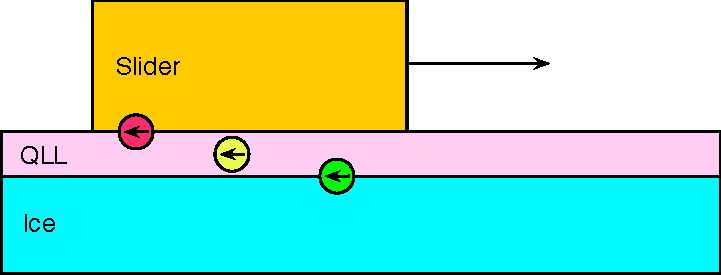
\includegraphics[width=4in]{Figures/QLLsketch}
\caption{\label{fig:QLLsketch} In the hydrodynamic regime, the
  friction felt by a slider on an ice surface is mediated by a
  quasi-liquid layer (QLL) that forms on the surface of the ice.
  There can be many contributions to this friction: capillary bridges
  between the slider and the QLL (red), viscous drag in the liquid
  (yellow), and solid / liquid friction between the ice and the liquid
  film (green). This study concerns the last of the three
  contributions, the drag contributed by the ice-liquid interface.}
\end{figure*}

Kietzig \textit{et al.} have outlined popular experimental techniques
used to investigate the coefficients of friction for a variety of
materials sliding on ice, as well as their sensitivity to temperature,
slider load, contact area, wettability and hydrophobicity of the
slider.\cite{Kietzig2010} Of particular interest, the friction
coefficients were found to increase with increasing slider
velocity. This was attributed to three physical processes; adhesion
forces between the slider's asperities and the ice surface, breaking
of capillary bridges between the slider and the ice surface, and the
viscous shearing of the ice melt across the ice surface. While teasing
apart the individual contributions has proven challenging,
Kietzig\cite{Kietzig2009} and Persson\cite{Persson2015,Tuononen2016}
have made significant progress. However, there is still very little
known about water shearing over ice surfaces. Open questions include:
how does the structure of the interface change during this process,
and what role does the presented crystal facet have in the observed
friction?


Observed coefficients of friction on ice are about 1 order of
magnitude lower than found for other solids. However, these
coefficients are found to vary with many factors, including
temperature, sliding speeds, surface asparities of the contact
surface, and load.\cite{Evans1976,Kietzig2002,Persson2001,Persson2015} While
holding all other contributions constant, the coefficient of friction
is observed to decrease with increasing sliding speeds. At slow
sliding speeds, the friction is found to be very large. Investigating
glass and granite sliding on ice around $10^{-7}$, Persson observed
coefficients of friction of 0.3 and 0.9 respectively.\cite{Persson2000} Li and
Somorjai attributed the discrepency in sliding speeds to be due to the
following; macroscopically at high sliding speeds frictional heating
causes surface melting, resulting in a lower coefficient of friction,
while microscopically the slider's surface asparities have less time
to push out the lubricating ice-melt and to cause large plastic
deformation on the ice surface.\cite{Li2007} They proposed the
opposite to hold true at smaller sliding speeds, thus the observed
increase in friction with decreasing sliding speeds.

Name and Name have observed a decrease in friction with increasing
temperature.\cite{Evans1976,Colbeck1997}. This is commonly attributed to a
thicker QLL present on the surface of ice with increasing temperature,
where the thicker QLL acts as a better lubricating layer. However, the
optimum temperature for speed skating is well known to be around -7
degrees Celcius, with a reported coefficient of friction of
0.0046.\cite{Dekoning1992} Above -7 degrees Celcius, the observed
friction is found to increase again, indicating that a plastic
deformation of the ice surface is causing an increase in the contact
area between the skate and the ice surface.\cite{Barnes1966,Barnes1971}
Since the load of the skater is not changing through this process, the
increase in the contact area yields a greater adhesive force and from
this the observed increase in friction.

\subsubsection{Atomic Force Microscopy Tip Penetration Measurements}
A quick intro of AFM...  Atomic force microscopy (AFM) is an
experimental technique in which an ultrafine metallic tip (with a
single atom at its point) is connected to a cantilever, and as the tip
approaches the surface, probes the surface topology by interpreting
the motion of the cantilever. BLAH. 

To probe the plastic deformation of ice surfaces, Pittenger \textit{et
  al.} have performed atomic force microscopy (AFM) experiments where
they indented the surface with the AFM tip.\cite{Butt2000,
  Pittenger2001,Bluhm2000} They found yield strengths of 14 MPa at -10.4
degrees Celcius, and 20 MPa at -15.1 degrees Celcius, both of which
are smaller than Young's modulus of bulk ice. This indicates that the
ice surface undergoes plastic deformation during the indentation of
the tip. Pettinger also attempted to determine the mechanism for
plastic flow during the plastic deformation by performing indentation
experiments at varying tip approach speeds. Butt \textit{et al.}
argued the rate of pressurized melting due to the presence of the tip
controlled the tip penetration speed.\cite{Butt2000} However, Pettinger
\textit{et al.} pointed out the pressure due to the tip was not large
enough to cause melting of the surface.\cite{Pittenger2001} Therefore, at the
temperatures and pressures Pettinger performed the AFM experiments at,
one would expect a thick QLL to be present. Given that, the
penetration rate should be governed by the rate of flow viscosity of
the QLL out from under the tip. However, the viscosity of the QLL
layer is still unknown. These AFM experiments do indicate that the
viscosity of the QLL must be at least 2 orders of magnitue greater
than that of bulk supercooled water. Li and Somorjai conjecture that
the increase in viscosity could be due to the confinement of the QLL
between the AFM tip and the ice, or due to the intrinsic ordering of
the QLL itself.

% Molecular dynamics simulation of ice indentation by model atomic
% force microscopy tips.
%  Constantin, Carignano, Corti, Szleifer, JPC-C 119 (2015) 27118

% end Constantin2015

\subsubsection{Lateral Force Microscopy Measurements}
Lateral force microscopy is an experimental technique in which ...

Using LFM, Bluhm \textit{et al.} have obtained friction coefficients
for ice grown on a mica substrate over a temperature range of -40 to
-24 degrees Celcius.\cite{Bluhm2000} Plotting the lateral force against the
imposed load, they were able to extract a friction coefficient of
about 0.6, which was robust over the entire temperature range
spanned. Due to this, and that the value obtained is comparable to
static friction observed in macroscopic measurements, they believe the
QLL was pushed out from under the tip, resulting in the tip having
direct contact with the ice surface. (They observed a QLL of about 8 nm thick
on the surface at XX degrees Celcius.) 

\subsubsection{Viscosity of the QLL}
 Interpretation of AFM measurements of the friction of ice depends
 strongly on whether a QLL is present between the tip and the
 surface. However, since the viscosity of the QLL is not known, nor
 how the value changes with changing conditions such as temperature or
 confinement under the tip, many of the results reported above are
 open to conjecture. A promising technique to obtain the viscosity of
 the QLL is interfacial force microscopy (IFM). The benefit to IFM as
 compared to other AFM techniques, is it does not suffer from the
 'jump-in' instability as it is  force-controlled (more). Using IFM,
 measurements of the normal and lateral forces are able to be obtained
 throughout the interfacial separation.\cite{Joyce1991} Recently, Name and
 Name have studied confined water between a Au(111) surface and a Au
 tip.\cite{Major2006} The effective viscosity was observed to be 7 orders of
 magnitude greater than bulk water, with the increase attributed to
 the structural ordering required under confinement. 

 It would be interesting if an IFM investigation of the QLL on ice is
 able to charactarize the viscosity of the ice-melt, which might help
 to further explain the observed AFM results described
 above. Similarly, knowledge of the viscosity would also help
 ellucidate the mechanism for the observed QLL behavior at the leading
 and trailing edge of sliders.

 % End Summary


% Determination of Surface Tension-to-Shear VIscosity Ratio for
% Quasiliquid layers on Ice Crystal Surfaces.
%   K. Murata, H. Asakawa, K. Nagashima, Y. Furukawa, G. Sazaki
%   PRL 115 (2015) 256103
Using laser confocal microscopy in conjunction with an inverted
optical microscope, Murata \textit{et al.} have recently measured the
characteristic-velocity (\textit{i.e.} the surface tension-to-shear
viscosity ratio) of two distinct wetting morphologies of QLLs on the
basal surface of ice at -0.2 degrees Celcius and a pressure of 578.9
Pa.\cite{Murata2015} They observed a partial wetting QLL, described as
a bulk liquid droplet (BLD), as well as a complete wetting state,
described as a thin liquid layer (TLL). The characterstic-velocity of
the BLDs was determined from relaxation modes of their contact lines,
which was observed to decay with single exponential behavior according
to
\begin{equation}
u_q = u_q(0) exp\Bigg(-\frac{V^* \theta^3 q}{3l}t\Bigg)
\end{equation}
where $q$ is the wave vector for the perturbing mode for the
relaxation of the amplitude of the contact line and $u_q(0)$ being the
initial amplitude of the mode. Here, $V^* = \gamma / \eta$ is the
characteristic velocity and $\theta$ is the contact angle the BLD makes
with the ice surface ($\sim$ 2 degrees). Lastly, the logarithmic factor
$l=\mathrm{ln}(L/a)$ is a cutoff parameter which helps avoid
singularities. From this fit, they obtained $V^* = 2 \pm 1$ m/s, which
is about an order of magnitude smaller than that of bulk water, 42.21
m/s.

Murata \textit{et al.} also investigated the spreading dynamics of the
BLD-QLLs, during the transformations to TLL-QLLs. The radii of the
spreading BLD-QLLs were fit to a power law
\begin{equation}
r = L (\frac{4S}{3Ll \eta})^{1/4}(t+t_0)^{1/4}.
\end{equation}
Here, $S$ is the spreading coefficient, and $t_0$ captures the initial
state of the droplet. As the QLL transitions from the BLD
drpolet-shape to the TLL pancake-shape, the volume must be
conserved. From this conservation, Murata \textit{et al.} estimated
the thickness of the TLLs as 9 $\pm$ 3 nm.

Lastly, Murata \textit{et al.} have obtained the characterstic
velocity of the TLLs in the same way as the BLDs. However, here the
hydrodynamic dissipation is not located at the wedge of the droplet
like in the BLD case, but instead the dissipation occurs within the
fluid of the pancake-shape object itself. Due to this, a slightly
different expression for the viscious force must be used, and the
resulting characteristic velocity was found to be $V^* = 0.2 \pm 0.1$
m/s, about 200 times smaller than that of bulk water. This seems to
imply a dependence on the characterstic velocity to the QLLs contact
area and distance from the surface. The BLD droplet-shaped QLLs (where
the QLL is only partially wets the surface and a larger amount of the
QLL resides further from the surface), were found to have a
characterstic velocity of about an order of magnitude larger than the
more completely wetting state, where more of the QLL resides closer to
the surface.

It is interesting to note that the surface tension of the BLD/air
interface ($\gamma_t$) is approximately equal to the TLL/air interface
surface tension ($\gamma_b$), as there is observed coexistence of both
forms of QLLs at the same time. Therefore, the discrepency in $V^*$
can be primarily attributed to the shear viscosity of the QLL phase.
% end Murata2015




%\subsection{Friction at Ice/Water Interfaces}
%%%%%%%%%%%%%%%%%%%%%%%%
% One anomoly is the reduced friction at ice/water interfaces, explain
% the slider problem. 
% Break down into the three contributions of friction, explain qll and role.
%
%%%%%%%%%%%%%%%%%%%%%%%%
% Ice/water interface
% ice/qll interface
%%%%%%%%%%%%%%%%%%%%%%%%

%iceWaterFriction intro
% Ice friction has been investigated extensively with a range
% of experimental techniques to elucidate the role of
% temperature,\cite{Bowden1939,Evans1976,Roberts1981,Derjaguin1988,Liang2003,Higgins2008} sliding speed,\cite{Evans1976,Derjaguin1988,Liang2003} applied
% load,\cite{Bowden1939,Oksanen1982,Derjaguin1988,Buhl2001,Baurle2006}
% contact area,\cite{Bowden1939,Baurle2007} and
% moisture.\cite{Calabrese1980} Kietzig \textit{et al.} performed
% experiments on steel alloy rings sliding over a prepared ice
% surface.\cite{Kietzig2009} They investigated the effect of surface
% nanopatterning, hydrophobicity, and surface structure of the
% ice-exposed slider on the ice / slider friction.
% Using laser irradiation, the slider surface hydrophobicity was tuned
% without changing the chemical nature of the material. Kietzig showed
% that laser-induced hydrophobicity resulted in fewer capillary bridges
% forming between the slider and a thin film of melted ice. This reduced
% the amount of viscous shearing of the ice-melt, resulting in a lower
% friction coefficient.
% While ice friction experiments have focused on heterogeneous
% materials,\cite{Bowden1939,Evans1976,Derjaguin1988,Liang2003,Liang2005,Baurle2006,Baurle2007,Kietzig2009,Kietzig2010}
% there have also been significant advances made in understanding
% ice-ice
% friction.\cite{Oksanen1982,Kennedy2000,Maeno2004,Fortt2007,Fortt2011,Lishman2011,Samadashvili2013}

% Experiments and computer simulations both suggest the existence of a
% quasi-liquid layer (QLL) that forms at the surface of ice at
% temperatures below the bulk melting point but above
% 235~K.\cite{Kroes1992,Ikeda-Fukazawa2004,Picaud2006,Conde2008,Bartels-Rausch2014,Sancheza2017}
% The formation of this layer is driven by the termination of the
% periodic crystal structure. The surface molecules are not as tightly
% bound to their lattice positions as molecules in the underlying ice,
% and with sufficient thermal energy, these molecules reorient to
% maximize hydrogen bonding. At warmer temperatures, they can also
% translate along the surface.\cite{Pfalzgraff2011,Bartels-Rausch2014}
% The existence of the QLL is now generally accepted as one of the
% reasons that ice displays a low coefficient of sliding
% friction.\cite{Dash1995,Rosenberg2005,Dash2006,Malenkov2009}

% Three distinct ice friction regimes have been described:
% boundary friction, mixed friction, and hydrodynamic friction, and the
% particular regime depends on the temperature and sliding velocity of
% the
% material.\cite{Bhushan2002,Kietzig2009,Kietzig2010,Persson2015,Tuononen2016}
% The observed friction is the result of different physical processes in
% each regime. In boundary friction, the lubricating layer of ice melt
% is only a few molecules thick. This thin film is unable to support the
% sliding load, and friction can be attributed to surface asperities of
% the sliding material interacting with the ice surface
% itself.\cite{Bhushan2002} In the mixed friction regime, the
% lubricating layer is thicker than in the boundary regime, but not yet
% sufficiently thick to maintain the sliding load. The QLL film reduces
% solid-solid adhesion at the interface, although the lubricating layer
% can also form capillary bridges with the material, resulting in a drag
% force.\cite{Kietzig2009,Kietzig2010}

% If the liquid layer is thick enough to support the sliding load, the
% slider's surface asperities are no longer in contact with the surface
% and the observed friction may be partially due to the capillary
% bridges formed between the ice melt and the material. Under these
% conditions, the ice friction is classified as hydrodynamic
% friction.\cite{Kietzig2009,Kietzig2010} Thus the three regimes are
% characterized by the extent that a liquid-like layer of water
% mitigates the sliding load.

% Kietzig \textit{et al.} have outlined popular experimental techniques
% used to investigate the coefficients of friction for a variety of
% materials sliding on ice, as well as their sensitivity to temperature,
% slider load, contact area, wettability and hydrophobicity of the
% slider.\cite{Kietzig2010} Of particular interest, the friction
% coefficients were found to increase with increasing slider
% velocity. This was attributed to three physical processes; adhesion
% forces between the slider's asperities and the ice surface, breaking
% of capillary bridges between the slider and the ice surface, and the
% viscous shearing of the ice melt across the ice surface. While teasing
% apart the individual contributions has proven challenging,
% Kietzig\cite{Kietzig2009} and Persson\cite{Persson2015,Tuononen2016}
% have made significant progress. However, there is still very little
% known about water shearing over ice surfaces. Open questions include:
% how does the structure of the interface change during this process,
% and what role does the presented crystal facet have in the observed
% friction?

% To help understand slider-ice friction in the hydrodynamic regime, we
% have simulated the drag forces contributed by the interaction of the
% liquid water film with the underlying ice facet. This study uses
% non-equilibrium molecular dynamics (with an applied momentum flux) to
% create a shear flow at the ice / water interface. The magnitude of the
% momentum flux is then used to compute the solid / liquid friction for
% four different facets of ice that are presented to the liquid.  We
% have previously used this technique to study solid / liquid friction
% for the basal and prismatic crystal facets where we observed
% significant facet-dependence, and noted surface corrugations that
% could contribute to these differences.\cite{Louden2013a} Here, we
% broaden the investigation to four common ice facets using two
% different water models, we study significantly larger systems for
% significantly longer times, a wider range of shear rates, and we
% introduce a novel method for calculating solid / liquid friction
% coefficients under conditions of \textit{negative} slip.


% end iceWaterFriction intro


\section{Summary}
We began this chapter with an overview of molecular dynamics
simulations, and followed with a discussion of the importance of water
in our world and in our lives.  In the chapters to follow, I present
my contribution to our understanding of the most anomalous molecule,
water. In Chapter \ref{chap:Methods} I describe the computational
details and methodologies used in simulating shearing at
ice-I$_\mathrm{h}$ / water interfaces. In Chapters \ref{chap:Str} and
\ref{chap:Dyn}, I investigate the structure and dynamics of the liquid
at the interface, and present estimates of the interfacial width. In
Chapter \ref{chap:Friction}, I present an appropriate friction
coefficient for no-slip boundary conditions, and explore possible
mechanisms of the observed facet dependent friction. In Chapter
\ref{chap:QLL}, I investigate the shear viscosity of the premelting
quasi-liquid layer of ice-I$_\mathrm{h}$ / vapor interface. Lastly, I
conclude my work and project towards the future in Chapter
\ref{chap:Concl}.



% Below here is text I've written and removed from the chapter, but
% don't want to lose to the delete key.


% Water plays a rich role in
% biochemical processes, where it has been seen to act as a solvent,
% reactant, product, catalyst, chaperone, messenger, and
% controller. Water also plays a dominant role in the complex folding of
% proteins.

% Our species is highly dependent on the solubility of gasses in liquid
% water. Beyond the movement of oxygen (O$_{2}$) throughout
% our bodies, much of the oxygen we breathe is produced by sea
% life. These marine plants require carbon dioxide
% (CO$_{2}$) in order for photosynthesis to produce
% carbohydrates and release oxygen. However, the solubility of gasses in
% water is highly sensative to temperature, pressure, and salinity. 

% Water molecules associate with each other relatively
% tightly. Therefore, H2O has relatively high values of surface tension,
% melting point, and boiling point.

% water has a relatively high surface tension, of 72.8 mN m−1 at room
% temperature, due to its high cohesion, the highest of the common
% nonionic, nonmetallic liquids.

%Pan 2010
% Pan \textit{et al.} calculated the surface energy, $\gamma$, using an
% \textit{ab initio} approach, through
% \begin{equation}\label{PanSurfaceEnergy}
% \gamma = \frac{E_{tot}^{slab}(n) - nE_{tot}^{bulk}}{2A}
% \end{equation}
% where $E_{tot}^{slab}$ is the total energy of the ice slab obtained
% from their DFT calculations, $n$ is the number of bilayers in the
% slab, and $A$ is the surface area of the exposed slab. The factor of
% two is present to account for the exposure of two surface upon
% cleaving a crystal. The bulk energy per bilayer, $E_{tot}^{bulk}$, is
% extrapolated from calculations with varying number of ice bilayers
% using 
% \begin{equation}
% E_{tot}^{bulk} = E_{tot}^{slab}(n) - E_{tot}^{slab}(n-1).
% \end{equation}
% This relation holds for ice slabs thicker than some critical
% thickness, as the energy of insertion of a bilayer is equivalent to
% that of a bilayer addition of bulk ice.

% On the energy of the bulk ice XI to bulk ice-I$_\mathrm{h}$ proton order to
% disorder transition, `` The energy difference on the level of
% ?5meV/H2O between the lowest energy ordered ice XI structure and the
% disordered ice-Ih structures is in the right ballpark for a bulk
% order–disorder transition of about 72 K. At the ice XI–Ih phase
% transition temperature (T), the ordering energy ?E should equal
% T?S,where ?S is the entropy difference between the ordered (ice XI)
% and disordered (ice-Ih) phases. In this system the entropy is
% comprised of two parts: vibrational and configurational entropy. The
% vibrational entropy differences between the two phases is expected to
% be almost negligible since the phonon frequencies of ice XI and Ih do
% not differ greatly, as has been seen through comparison of calculated
% phonon dispersion curves of ice XI with experimental phonon dispersion
% curves of ice-Ih [36, 37]. Thus the phase transition temperature is
% governed primarily by differences in configurational entropies,
% something which Pauling has shown to be given by Sconf = kB ln( 3 2 )
% = 0.035 meV/(K·H2O) [15].  Hence at the phase transition temperature,
% the configurational entropy contributes 2–3 meV/H2O, which is
% consistent with the ?5meV/H2O total energy difference between the two
% phases. Therefore'' ``Knight et al [17] who neglected the vibrational
% contribution to the entropy and predicted a bulk transition
% temperature of ca. 100 K based on DFT calculations.''

% Pan observed that OH bonds sticking
% out on the surface moved away slightly from their initial position, to
% ``lean'' away from one another as much as possible.

% Initially Fletcher\cite{Fletcher} and later Buch\cite{Buch} observed
% the OH bonds ``dangling'' from the surface play an important role in
% the energetics of the surface. To quantify unique distributions of
% dangling OH bonds, Pan \textit{et al.} calculated an order parameter
% which describes the average separation between dangling OH bonds at
% the surface.
% \begin{equation}
% C_{OH}^{basal} = \frac{1}{N_{OH}}\sum_{i=1}^{N_{OH}}c_{i}
% \end{equation}
% where $N_{OH}$ is the total number of dangling OH bonds presented by
% the two basal surfaces, and $c_{i}$ is the number nearest neighbor
% dangling OH bonds around the $i$th dangling OH bond. Here we see that
% a larger value of $C_{OH}^{basal}$ indicate a more inhomogeneous
% distribution of dangling OH bonds, and that on average the dangling OH
% groups are close together. For a completely random distribution of
% dangling OH bonds, the order parameter will go to $\approx 3$, and the
% smallest value that can be obtained for a non-polar surface is 2.

% Plotting surface energy as a function of $C_{OH}$, a linear
% relationship is obtained. This indicates that as the more inhomogenous
% surface dangling OH patterning results in a larger surface energy.

%end Pan et al.

%%%%%%%%%%%%%%%%%%%%%%%%%%%%%%%%%%%%%%%%%%%%%%%%%%%%%%%%%%%%%%%%%%%%%%%%%%%%%%%%%%%
%		CHAPTER 2 -- System Contruction & Computational Details
%%%%%%%%%%%%%%%%%%%%%%%%%%%%%%%%%%%%%%%%%%%%%%%%%%%%%%%%%%%%%%%%%%%%%%%%%%%%%%%%%%%


\chapter{CONSTRUCTING AND SHEARING ICE-I$_\mathrm{h}$ / WATER INTERFACES}

\begin{flushright}
\textit{''Why do snowflakes always fall as flat structures with six corners?''} \\
-Joannes Kepler (1611) \\
\end{flushright}


Non-equilibrium molecular dynamics simulations of solid / liquid
friction at the basal $\{0001\}$, prismatic $\{10\bar{1}0\}$,
14\degree~pyramidal $\{20\bar{2}1\}$, and secondary prism
$\{11\bar{2}0\}$ facets of an ice-I$_\mathrm{h}$ crystal were
performed. Contained in this chapter are the details of how the
systems were constructed as well as the computational details
followed. In addition, non-equilibrium molecular dynamics
methodologies and water models are discussed.


\section{Construction of Ice I$_\mathrm{h}$ / Water Interfaces}

Ice-I$_\mathrm{h}$ crystallizes in the hexagonal space group
P$6_3/mmc$, and ice crystals normally form hexagonal plates with the
basal face, $\{0001\}$, forming the top and bottom of each plate, and
the prismatic facet, $\{10\bar{1}0\}$, forming the sides.  In extreme
temperatures or low water saturation conditions, ice crystals can form
hollow columns, needles, and dendrites, exposing other crystalline
facets of the ice to the surroundings.  Among the more
commonly-observed facets are the secondary prism, $\{11\bar{2}0\}$,
and the two pyramidal, 14\degree~$\{20\bar{2}1\}$ and
28\degree~$\{10\bar{1}1\}$, faces. Images of these surfaces can
be found in Fig. \ref{fig:surfMorph}.


\begin{figure}
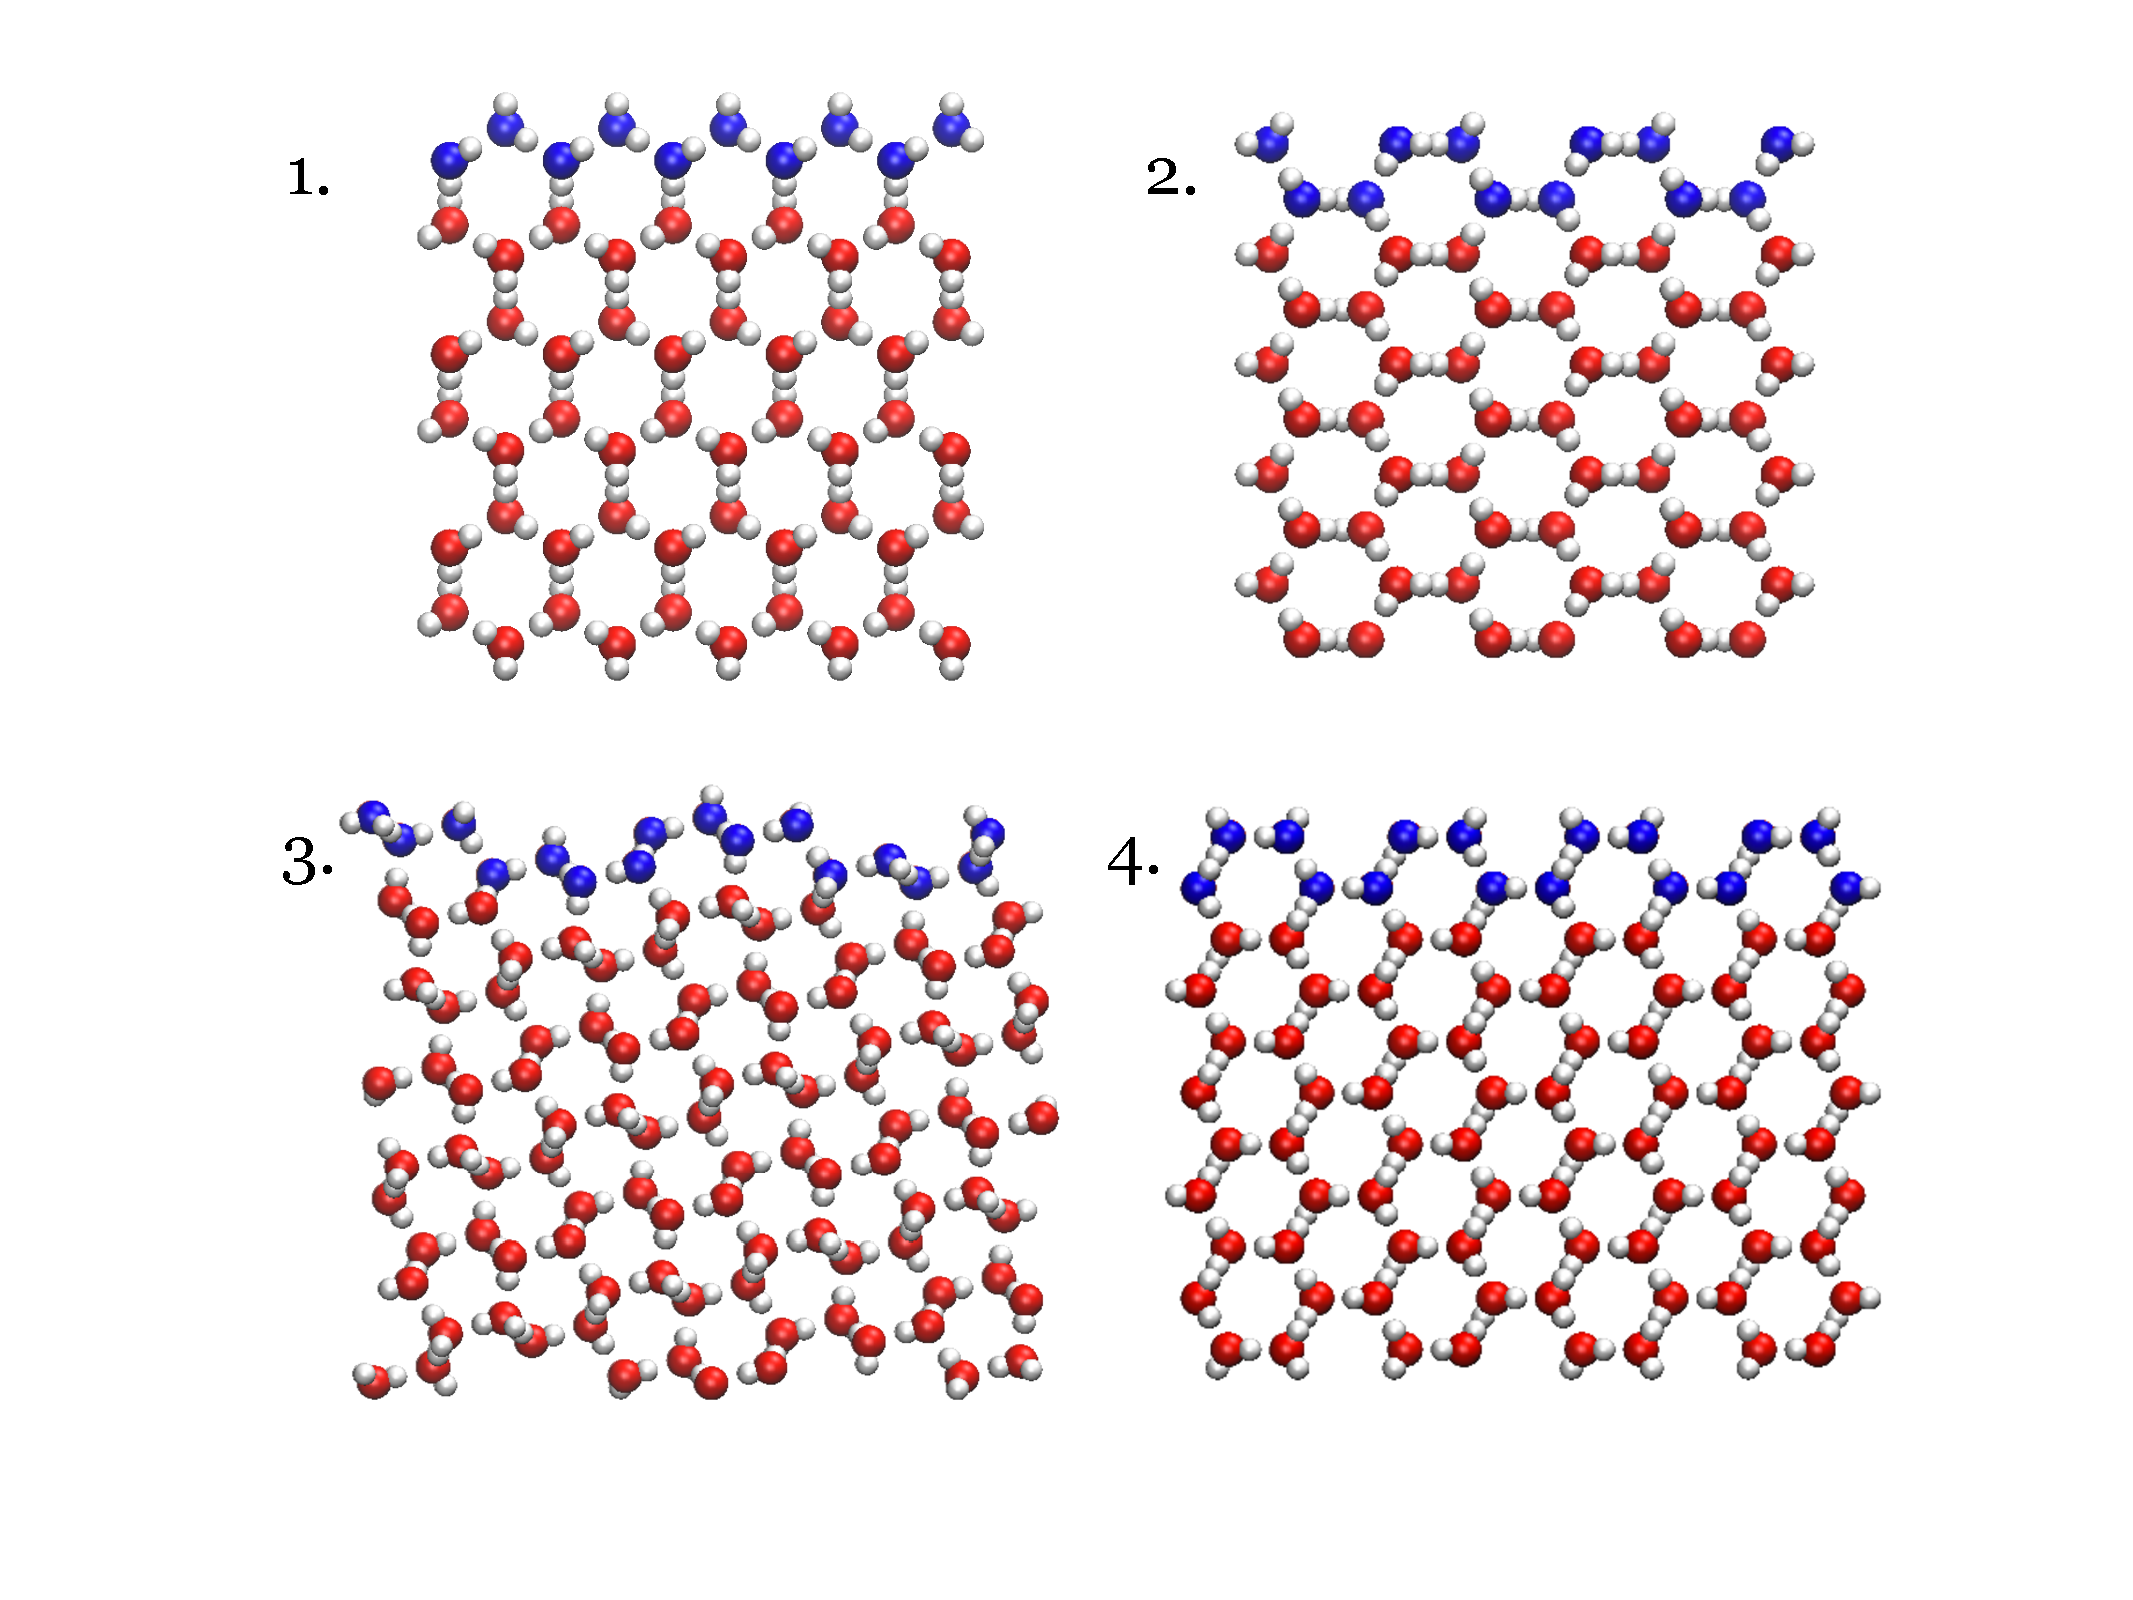
\includegraphics[width=1.0\linewidth]{Figures/surfMorph}
\caption{\label{fig:surfMorph}The basal (1), prismatic (2), pyramidal
  (3), and secondary prism (4) facets of an ice-I$_\mathrm{h}$
  crystal, generated by replication of unit cell structure 6 by Hirsch
  and Ojam\"{a}e. Left column and middle column: the two perpindicular
  side-on views of the crystal facet. Right column: looking down on
  the crystal face. The surface oxygens have been colored blue for
  clarity.}
\end{figure}

Surface energies, dimensions of crystal channels at zero kelvin, ...

The oxygen lattice is a hexagonal unit cell comprising 4 oxygen atoms,
but it is also possible to construct an equivalent orthorhombic unit
cell with 8 oxygen atoms.\cite{Hirsch2004} Hydrogen atom placement
obeys the Bernal-Fowler ice rules which distribute protons so that
each oxygen donates two hydrogen bonds and accepts two from
neighboring molecules.\cite{Bernal1933} The resulting structure also
typically has zero net dipole moment. Below 72~K and under ambient
pressures, the lattice can undergo a phase transition to ice XI, a
configuration with ferroelectric proton-ordering and a non-zero bulk
dipole moment (see Fig. \ref{fig:iceTransition}).

\begin{figure}
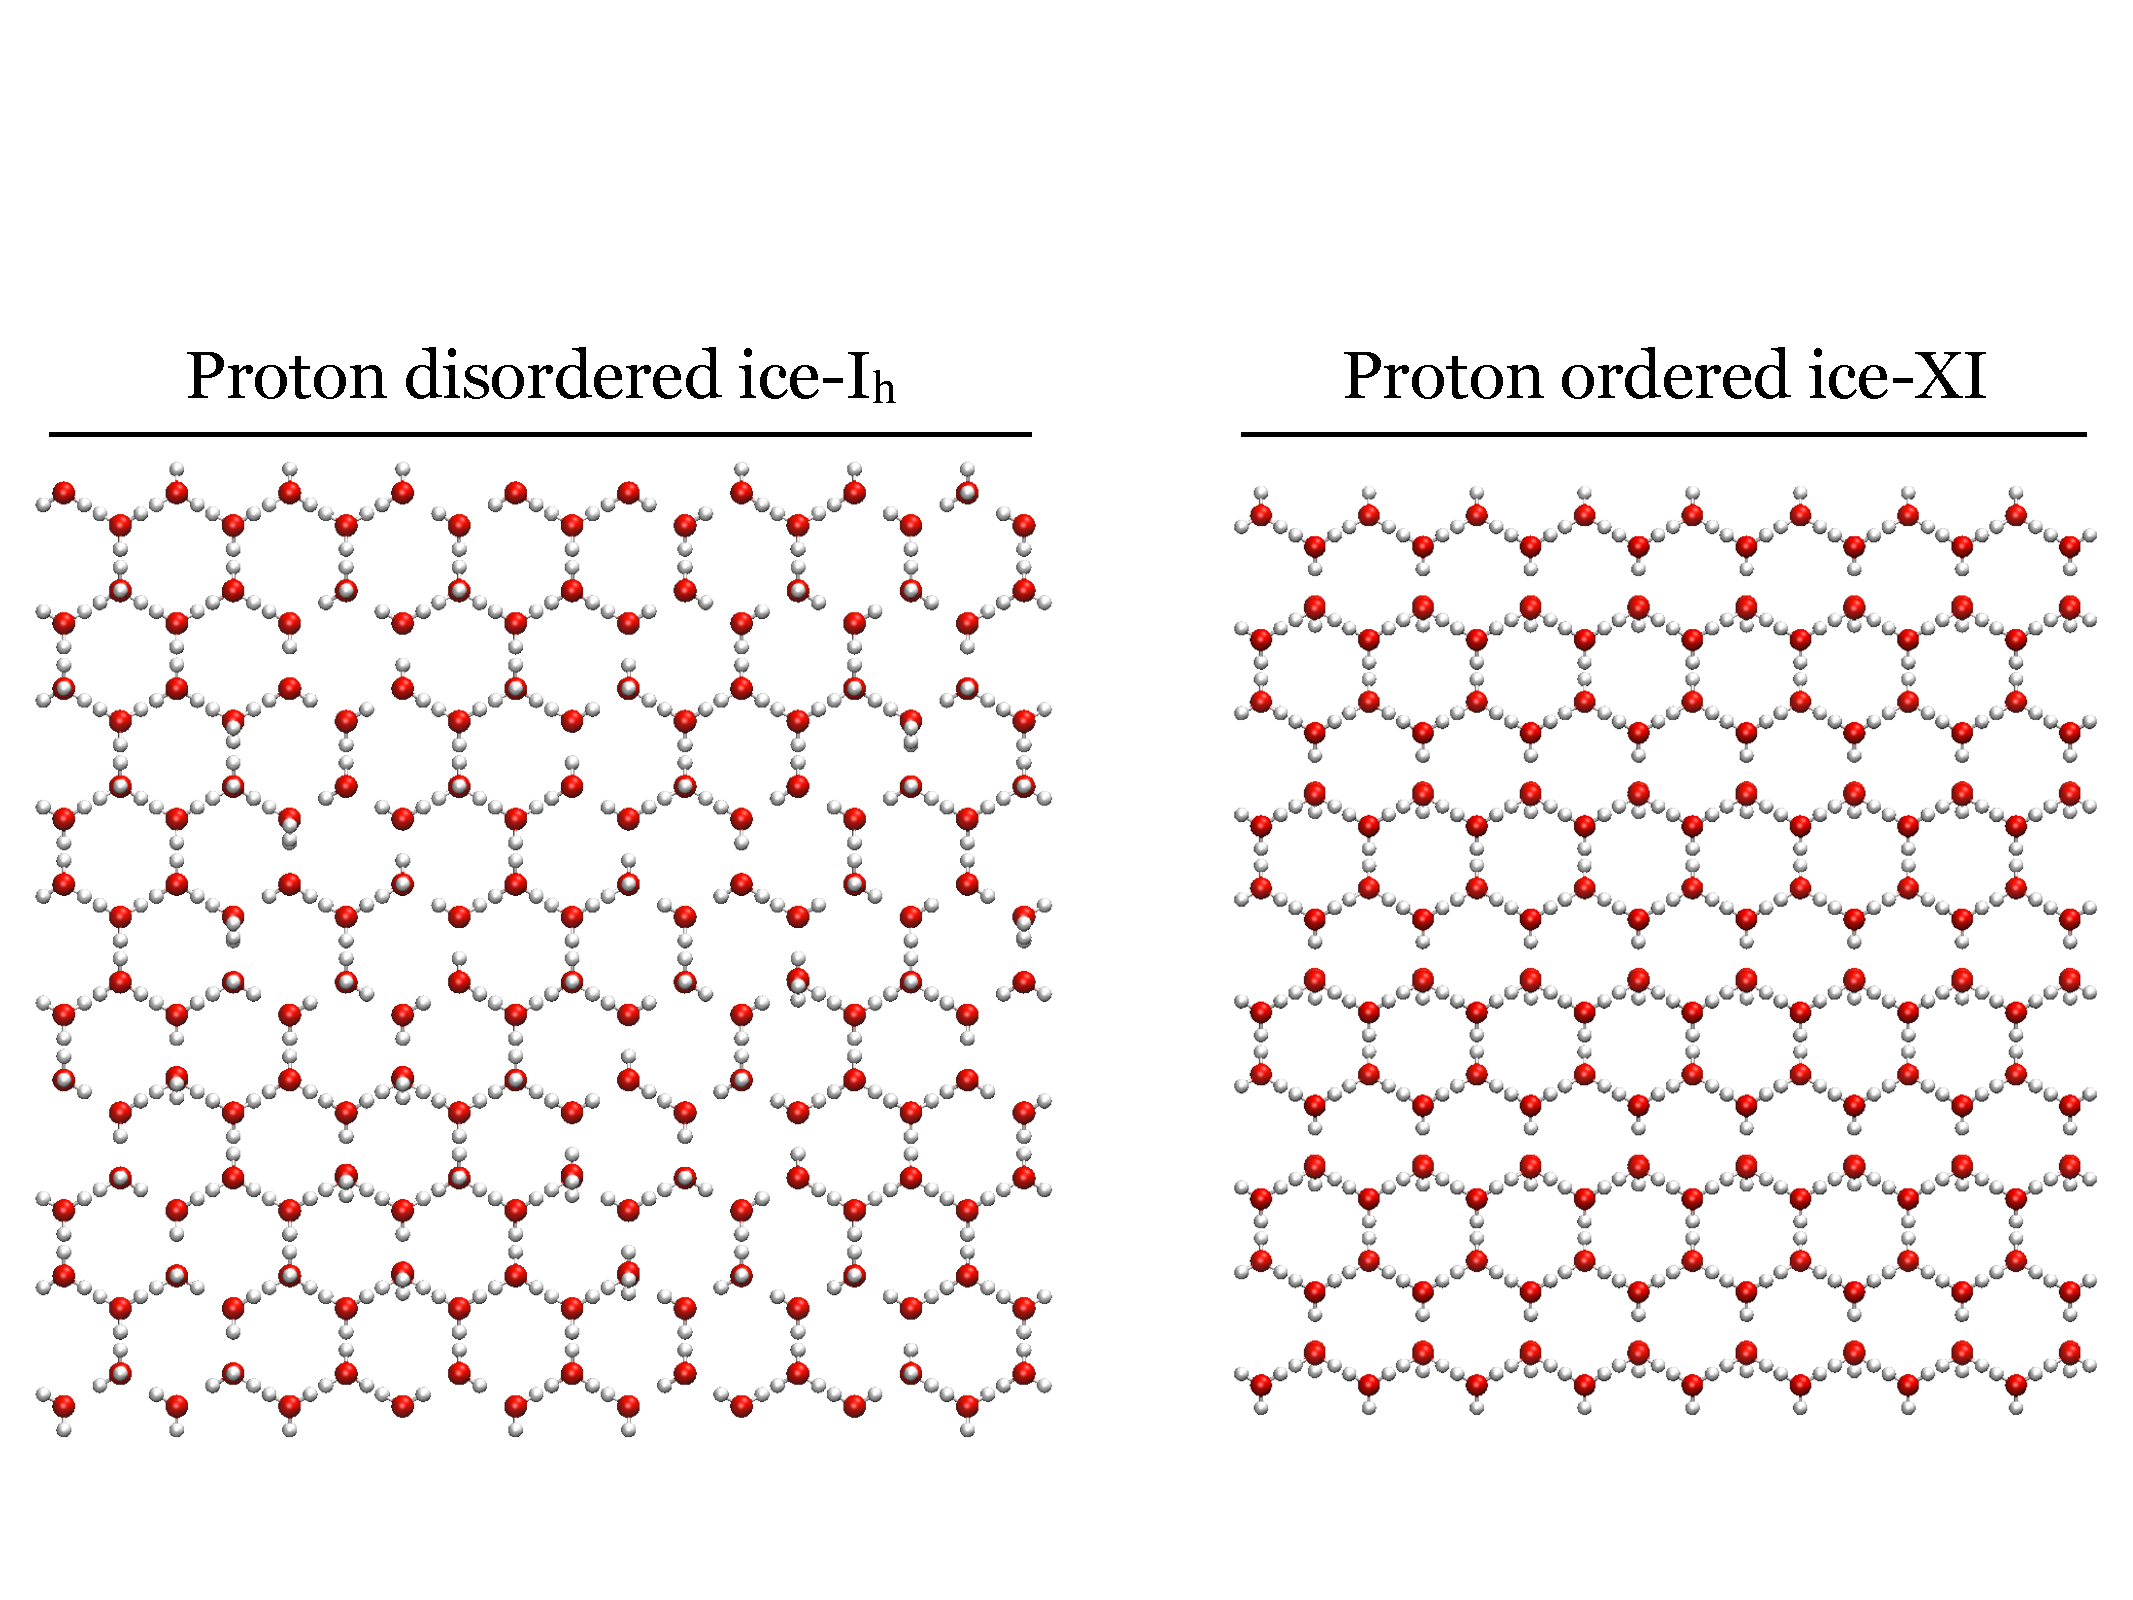
\includegraphics[width=\linewidth]{Figures/iceTransition}
\caption{\label{fig:iceTransition}Left: A proton-disordered
  ice-I$_\mathrm{h}$ crystal, viewed down onto the basal
  facet. Coordinates for this crystal structure are taken from
  Hayward and Reimers.\cite{Hayward1997} Right:
  A proton-ordered ice-XI crystal, viewed down on the same crystal
  face. Coordinates for this structure are taken from Structure 1 of
  Hirsch and Ojam\"{a}e.\cite{Hirsch2004} The phase transition between
ice-I$_\mathrm{h}$ and ice-XI is believed to be $\sim$ 72~K.}
\end{figure}

While exploring the ice-I$_\mathrm{h}$ to XI phase transition, Hirsch
and Ojam\"{a}e determined sixteen unique hydrogen arrangements for the
ice-I$_\mathrm{h}$ orthorhombic unit cells.\cite{Hirsch2004} Upon
replication of some of these unit cells, the resulting structures
present stripes of dangling H-atoms and lone pairs at an exposed
crystal facet. These orthorhombic initial configurations can be used
to reproduce the surface features from Buch \textit{et
  al.}\cite{Buch2008} that helped interpret sum-frequency generation
(SFG) experiments by the Shultz lab.\cite{Groenzin2007} More recently,
Nojima \textit{et al.}\cite{Nojima2017} have successfully obtained
both the real and imaginary parts of the vibrational spectra of the
free OH stretch for surface water molecules of the basal, prismatic,
and secondary prismatic facets at ca. 130~K through
heterodyne-detected sum-frequency generation (HD-SFG). They also
present evidence of proton-striped surfaces as the sign of the
imaginary part of the vibrational spectra indicates ``up'' or ``down''
orientations of surface molecules.

\begin{table}[h]
\centering
  \caption{MAPPING BETWEEN THE MILLER INDICES OF FOUR FACETS OF ICE IN
    THE $P6_3/mmc$ CRYSTAL SYSTEM TO THE ORTHORHOMBIC $P2_12_12_1$
    SYSTEM IN REFERENCE \bibpunct{}{}{,}{n}{}{,} \protect\citep{Hirsch04}.}
\label{tab:equiv}
\begin{tabular}{|ccc|} \hline
 & hexagonal & orthorhombic \\
 & ($P6_3/mmc$) & ($P2_12_12_1$) \\
 crystal face  & Miller indices & equivalent \\ \hline
basal & $\{0~0~0~1\}$ & $\{0~0~1\}$ \\
prism & $\{1~0~\bar{1}~0\}$ & $\{1~0~0\}$ \\
secondary prism & $\{1~1~\bar{2}~0\}$ & $\{1~3~0\}$ \\
pyramidal & $\{2~0~\bar{2}~1\}$ & $\{2~0~1\}$ \\ \hline
\end{tabular}
\end{table}

SPC/E~\cite{Berendsen1987} and TIP4P/Ice~\cite{Abascal2005} structures
were created starting from Structure 6 of Hirsch and Ojam\"{a}e's set
of orthorhombic representations for ice-I$_{h}$.\cite{Hirsch2004}
Replication of Structure 6 (unit cell geometry $P2_12_12_1$) produces a proton-ordered
version of ice I$_\mathrm{h}$ on a smaller length scale than the
simulation box. However, the resulting crystal has a zero-net dipole,
unlike proton ordered ice-XI crystals. Table \ref{tab:equiv} contains a
mapping between the Miller indices of common ice facets in the
P$6_3/mmc$ crystal system and those in the Hirsch and Ojam\"{a}e
$P2_12_12_1$ system.

Structure 6 from the Hirsch and Ojam\"{a}e paper has lattice
parameters $a = 4.49225$ \AA\ , $b = 7.78080$ \AA\ , $c = 7.33581$
\AA\ and two water molecules whose atoms reside at fractional
coordinates given in table
\ref{tab:p212121}. 

\begin{table}[h]
\centering
  \caption{FRACTIONAL COORDINATES FOR WATER IN THE ORTHORHOMBIC
    $P2_12_12_1$ SYSTEM FOR ICE I$_\mathrm{h}$ IN REFERENCE \bibpunct{}{}{,}{n}{}{,} \protect\citep{Hirsch0404}.}
\label{tab:p212121}
\begin{tabular}{|cccc|}  \hline
atom type & x & y & z \\ \hline
 O & 0.7500 & 0.1667 & 0.4375 \\
 H & 0.5735 & 0.2202 & 0.4836 \\
 H & 0.7420 & 0.0517 & 0.4836 \\
 O & 0.2500 & 0.6667 & 0.4375 \\
 H & 0.2580 & 0.6693 & 0.3071 \\
 H & 0.4265 & 0.7255 & 0.4756 \\ \hline
\end{tabular}
\end{table}


In order to generate large crystals for simulation, the primitive unit
cell was replicated in all dimensions. The crystal was cleaved along
the desired face, and two additional mutually perpendicular cuts were
made.  The crystal was reoriented so that the initial cut (basal,
pyramidal, prismatic, or secondary prism) was normal to the $z$-axis
of the simulation cell.  The resulting structures were extended in $x$
and $y$ to form large exposed facets in rectangular box geometries.
Because the orthorhombic unit cells are relatively small, using these
as building blocks for an ice simulation creates proton translational
order on the length scale of the unit cells. We note that all
simulated ice structures have proton ordering on the length scale of
the periodic box, but in order to reproduce proton surface striping
with zero dipole crystals, we have utilized proton translational
ordering on a smaller length scale than other ice studies.

Liquid water boxes were created with identical dimensions (in $x$ and
$y$) as the ice, with a $z$ dimension of three times that of the ice
block, and with a density corresponding to $1$ g / cm$^3$.  Each of
the ice slabs and water boxes were independently equilibrated to
$50$~K and a pressure of $1$ atm by coupling the temperature and
pressure of the system to a heat and pressure bath. For all
simulations non-bonded interactions were cut-off at 12~\AA~ and
electrostatics were handled using the damped-shifted force real-space
electrostatic kernel.\cite{Fennell2006} The resulting systems were
merged by carving out any liquid water molecules within 3~\AA~ of any
atoms in the ice slabs.  For the SPC/E simulations, the combined ice /
water systems were equilibrated to 225~K. The liquid-ice coexistence
temperature for SPC/E water has been reported as
$215 \pm 4$~K.\cite{Vega2006a,Fernandez2006} We observed a coexistence
temperature of 225~K for our crystals, possibly due to the surface
striped structures utilized in this study. For the TIP4P/Ice
simulations, the combined ice / water system was equilibrated to the
reported coexistence temperature, 270~K.\cite{Vega2006a,Fernandez2006}
The quiescent ice / water interfaces were then equilibrated for 10 ns,
with 5 ns under a constant temperature (NVT) integrator, followed by 5
ns under a microcanonical (NVE) integrator.  During this time the ice
was monitored for crystal growth or melting. We observed no advance of
the ice interface into the liquid, and no loss of crystallinity of the
ice. Reference \citen{Louden2013a} contains a more detailed
explanation of the construction of similar ice / water interfaces. The
resulting dimensions as well as the number of ice and liquid water
molecules contained in each of these systems are shown in Table
\ref{tab:sizes}.  Note that the water molecules are not restrained in
any way - molecules that start in the liquid phase may exchange with
the ice (and vice versa).

\begin{table}[h]
\centering
\caption{SIZES OF THE ICE / WATER SHEARING SIMULATIONS. (Box
  dimensions are given in \AA)\label{tab:sizes}}
\begin{tabular}{r|cc|ccc|ccc}
\toprule
 & & & \multicolumn{3}{c|}{SPC/E~(225~K)} &  \multicolumn{3}{c}{TIP4P/Ice~(270~K)}\\
 Interface & $N_\mathrm{ice}$ &
 $N_\mathrm{liquid}$ & $L_x$ & $L_y$ & $L_z$ & $L_x$ & $L_y$ & $L_z$ \\
\midrule
Basal  $\{0001\}$                 & 900 & 1846  & 23.87 & 35.83 & 98.64  & 23.37 & 38.83 & 97.67  \\
Prismatic  $\{10\bar{1}0\}$       & 3000 & 5464 & 35.95 & 35.65 & 205.77 & 36.33 & 38.86 & 191.75 \\
Pyramidal  $\{20\bar{2}1\}$       & 1216 & 2203 & 37.47 & 29.50 & 93.02  & 37.16 & 30.19 & 97.65  \\
Secondary Prism  $\{11\bar{2}0\}$ & 3840 & 8176 & 71.87 & 31.66 & 161.55 & 72.90 & 32.06 & 165.17 \\
\bottomrule
\end{tabular}
\end{table}


The liquid-state viscosity of the SPC/E water model has been
extensively characterized over a wide range of liquid
conditions~\cite{Kuang2012}, and its phase diagram has been well
studied~\cite{Baez1995,Bryk2004,Sanz2004a,Fennell2005}. With longer
cutoff radii and careful treatment of electrostatics, SPC/E mostly
avoids metastable crystalline morphologies like
ice-\textit{i}~\cite{Fennell2005} and ice-B~\cite{Baez1995}, although
Sanz \textit{et al.}\cite{Sanz2004a} found that the stable polymorph
for this model is likely ice-II at this temperature and 1 bar. The
free energies and melting
points~\cite{Baez1995,Arbuckle2002,Gay2002,Bryk2002,Bryk2004,Sanz2004a,Fennell2005,Fernandez2006,Abascal2007,Vrbka2007}
of various other crystalline polymorphs have also been calculated.
Haymet \textit{et al.}\cite{Bryk2002} have studied quiescent
ice-I$_\mathrm{h}$ / water interfaces using the SPC/E water model, and
have seen structural and dynamic measurements of the interfacial width
that agree well with both experimental results and more expensive
water models, although the coexistence temperature for SPC/E is still
well below the experimental melting point of real water.  

Recent investigations have questioned the applicability of SPC/E in
ice / water simulations,\cite{Vega2005c,Vega2011a,Gladich2012,Gallo2016}
however, so simulations have also been done using
TIP4P/Ice.\cite{Abascal2005} This model was parameterized by fitting
the equation of state, as well as the melting and coexistence lines
involving different ice polymorphs, and the resulting melting
temperature of ice-I$_\mathrm{h}$ is much closer to the experimental
value.\cite{Abascal2005} Although TIP4P/Ice is more computationally
demanding, it is worthwhile to compare models where liquid water is in
contact with ice at multiple coexistence temperatures.

\section{Shearing Ice I$_\mathrm{h}$ / Water Interfaces Without Bulk Melting}

As a solid is dragged through a liquid, there is frictional heating
that will act to melt the interface.  Close to the melting point of the
solid, this frictional heating may result in melting of the crystal.
We are interested in the structure and dynamics of the interface at
the coexistence temperature.  This can be accomplished using the velocity
shearing and scaling (VSS) variant of reverse non-equilibrium
molecular dynamics (RNEMD), which utilizes a series of simultaneous
velocity exchanges between two regions within the simulation
cell.\cite{Kuang2012} One of these regions is centered within the ice
slab, while the other is centrally located in the liquid
region. VSS-RNEMD provides a set of conservation constraints for
creating either a momentum flux or a thermal flux (or both
simultaneously) between the two slabs.  Satisfying the constraint
equations ensures that the new configurations are sampled from the
same NVE ensemble as before the VSS move.

The VSS moves are applied periodically to scale and shift the particle
velocities ($\mathbf{v}_i$ and $\mathbf{v}_j$) in two slabs ($H$ and
$C$) which are separated by half of the simulation box,
\begin{displaymath}
\begin{array}{rclcl}

 & \underline{\mathrm{shearing}} & &
 \underline{~~~~~~~~~~~~\mathrm{scaling}~~~~~~~~~~~~} \\
\mathbf{v}_i \leftarrow & 
  \mathbf{a}_c\ & + & c\cdot\left(\mathbf{v}_i - \langle\mathbf{v}_c
  \rangle\right)  +  \langle\mathbf{v}_c\rangle \\
\mathbf{v}_j \leftarrow & 
  \mathbf{a}_h & + & h\cdot\left(\mathbf{v}_j - \langle\mathbf{v}_h
    \rangle\right) + \langle\mathbf{v}_h\rangle .

\end{array}
\end{displaymath}
Here $\langle\mathbf{v}_c\rangle$ and $\langle\mathbf{v}_h\rangle$ are
the center of mass velocities in the $C$ and $H$ slabs, respectively.
Within the two slabs, particles receive incremental changes or a
``shear'' to their velocities.  The amount of shear is governed by the
imposed momentum flux, $\mathbf{j}_z(\mathbf{p})$
\begin{eqnarray}
\mathbf{a}_c & = & - \mathbf{j}_z(\mathbf{p}) \Delta t / M_c \label{vss1}\\
\mathbf{a}_h & = & + \mathbf{j}_z(\mathbf{p}) \Delta t / M_h \label{vss2}
\end{eqnarray}
where $M_{\{c,h\}}$ is the total mass of particles within each of the
slabs and $\Delta t$ is the interval between two separate operations.

To simultaneously impose a thermal flux ($J_z$) between the slabs we
use energy conservation constraints,
\begin{eqnarray}
K_c - J_z\Delta t & = & c^2 (K_c - \frac{1}{2}M_c \langle\mathbf{v}_c
\rangle^2) + \frac{1}{2}M_c (\langle \mathbf{v}_c \rangle + \mathbf{a}_c)^2 \label{vss3}\\
K_h + J_z\Delta t & = & h^2 (K_h - \frac{1}{2}M_h \langle\mathbf{v}_h
\rangle^2) + \frac{1}{2}M_h (\langle \mathbf{v}_h \rangle +
\mathbf{a}_h)^2 \label{vss4}.
\label{constraint}
\end{eqnarray}
Simultaneous solution of these quadratic formulae for the scaling
coefficients, $c$ and $h$, will ensure that the simulation samples from
the original microcanonical (NVE) ensemble.  Here $K_{\{c,h\}}$ is the
instantaneous translational kinetic energy of each slab.  At each time
interval, it is a simple matter to solve for $c$, $h$, $\mathbf{a}_c$,
and $\mathbf{a}_h$, subject to the imposed momentum flux,
$j_z(\mathbf{p})$, and thermal flux, $J_z$, values.  Since the VSS
operations do not change the kinetic energy due to orientational
degrees of freedom or the potential energy of a system, configurations
after the VSS move have exactly the same energy (and linear
momentum) as before the move.

As the simulation progresses, the VSS moves are performed on a regular
basis, and the system develops a thermal and/or velocity gradient in
response to the applied flux.  In a bulk material, it is quite simple
to use the slope of the temperature or velocity gradients to obtain
either the thermal conductivity or shear viscosity,
$\eta$.\cite{Bordat2002a}
\begin{equation}
\label{eq:viscosity}
j_z(p_x) = -\eta \left(\frac{\partial v_x}{\partial z}\right).
\end{equation}
At interfaces between dissimilar materials, the same method can be
used to extract \textit{interfacial} transport properties (e.g. the
hydrodynamic slip length or the interfacial thermal
conductance).


The VSS-RNEMD approach is versatile in that it may be used to
implement thermal and shear transport simultaneously.  Perturbations
of velocities away from the ideal Maxwell-Boltzmann distributions are
minimal, as is thermal anisotropy.  This ability to generate
simultaneous thermal and shear fluxes has been previously utilized to
map out the shear viscosity of SPC/E water over a wide range of
temperatures (90~K) with a single 1~ns simulation.\cite{Kuang2012}

Once thermal gradients had stabilized, linear momentum fluxes were
imposed coincident with the kinetic energy flux. The resulting
velocity gradients were allowed to stabilize for 1~ns before data
collection began. Four successive 1~ns simulations were performed for
each shear rate (varying from
$0.5 \rightarrow 10.0~\mathrm{~m~s}^{-1}$) . All atomic configurations
(positions and velocities) were saved every 1~ps, while statistical
measures of the system (e.g. temperature, potential energy, total
energy, and pressure) were sampled every 0.1~ps during the
simulation. Velocity and thermal profiles (used to compute friction)
were sampled every 2~fs. Small variations in the measured interfacial
widths between successive simulations were observed, but there was no
indication of bulk melting or crystal growth. That is, no large scale
changes in the positions of the two interfaces were observed during
the simulations. A representative configuration of the solvated
prismatic facet being sheared through liquid water is shown in Figure
\ref{fig:Shearing}.

\begin{figure}
\includegraphics[width=1.9in]{Figures/Shearing}
\caption{\label{fig:Shearing} Computational model of a slab of ice
  being sheared through liquid water.  The ice presents two copies of
  the prismatic $\{10\bar{1}0\}$ facet towards the liquid phase.  The
  RNEMD simulation exchanges both linear momentum (indicated with
  arrows) and kinetic energy between the central box and the box that
  spans the cell boundary.  The system responds with weak thermal
  gradient and a velocity profile that shears the ice relative to the
  surrounding liquid.}
\end{figure}

\section{Computational Details}
All simulations were performed using OpenMD,\cite{OOPSE,openmd} with a
time step of 2 fs and periodic boundary conditions in all three
dimensions.  Electrostatics were handled using the damped-shifted
force real-space electrostatic kernel.\cite{Ewald} When applicable,
VSS-RNEMD moves were attempted every time step. This minimized the
magnitude of individual momentum exchanges.  Forcefield parameters for
both water models can be found in table \ref{tab:waterModels}.

\begin{table}[H]
\centering
\caption{FORCEFIELD PARAMETERS FOR THE SPC/E AND TIP4P/Ice WATER MODELS.}
\label{tab:waterModels}
\begin{tabular}{|l|c|c|c|c|c|c|c|c|} 
\hline
  Model &  $\sigma$ (\AA) & $\epsilon$ (kJ $\mathrm{mol}^{-2}$) &
                                                              $\mathrm{l}_{1}$
                                                              (\AA) &
                                                                    $\mathrm{l}_{2}$
                                                                      (\AA)
  & $\mathrm{q}_{1}$ (e) & $\mathrm{q}_{2}$ (e) & $\theta$
                                                  ($^{\mathrm{o}}$) &
                                                                      $\phi$ ($^{\mathrm{o}}$) \\ \hline
  SPC/E & 3.166 & 0.650 & 1.000 & - & +0.4238 & -0.8476 & 109.47 & - \\
  TIP4P/Ice & 3.1668 & 0.8822 & 0.9572 & 0.1577 & +0.5897 & -1.1794 &
  104.52 & 52.26 \\
\hline
\end{tabular}
\end {table}


The interfaces were equilibrated for a total of 10 ns at equilibrium
conditions before being exposed to either a shear or thermal gradient.
This consisted of 5 ns under a constant temperature (NVT) integrator
set to 225K followed by 5 ns under a microcanonical integrator.  Weak
thermal gradients were allowed to develop using the VSS-RNEMD (NVE)
integrator using a small thermal flux ($-2.0\times 10^{-6}$
kcal/mol/\AA$^2$/fs) for a duration of 5 ns to allow the gradient to
stabilize.  The resulting thermal gradients ($< 10$~K over the length
of the simulation box) were allowed to stabilize for 5 ns, and were
found to be sufficient to keep the interface within $\pm 5$ K of the
target temperature (225~K for SPC/E and 270~K for TIP4P/Ice) during
all shearing simulations.


Velocity gradients were then imposed using the VSS-RNEMD (NVE)
integrator with a range of momentum fluxes.  These gradients were
allowed to stabilize for 1~ns before data collection began. Once
established, four successive 0.5~ns runs were performed for each shear
rate.  During these simulations, snapshots of the system were taken
every 1~ps, and statistics on the structure and dynamics in each bin
were accumulated throughout the simulations.  Although there was some
small variation in the measured interfacial width between succcessive
runs, no indication of bulk melting (or crystallization) was observed.





% \section{Results and discussion}

% \subsection{Interfacial width}
% Any order parameter or time correlation function that changes as one
% crosses an interface from a bulk liquid to a solid can be used to
% measure the width of the interface.  In previous work on the ice/water
% interface, Haymet {\it et al.}\cite{Bryk02} have utilized structural
% features (including the density) as well as dynamic properties
% (including the diffusion constant) to estimate the width of the
% interfaces for a number of facets of the ice crystals.  Because
% VSS-RNEMD imposes a lateral flow, parameters that depend on
% translational motion of the molecules (e.g. diffusion) may be
% artificially skewed by the RNEMD moves.  A structural parameter is not
% influenced by the RNEMD perturbations to the same degree. Here, we
% have used the local tetrahedral order parameter as described by
% Kumar\cite{Kumar09} and Errington\cite{Errington01} as our principal
% measure of the interfacial width.  A previous study by Bryk and Haymet
% also used local tetrahedrality as an order parameter for ice/water
% interfaces.\cite{Bryk2004b}

% The local tetrahedral order parameter, $q(z)$, is given by
% \begin{equation}
% q(z) = \int_0^L \sum_{k=1}^{N} \Bigg(1 -\frac{3}{8}\sum_{i=1}^{3}
% \sum_{j=i+1}^{4} \bigg(\cos\psi_{ikj}+\frac{1}{3}\bigg)^2\Bigg)
% \delta(z_{k}-z)\mathrm{d}z \Bigg/ N_z
% \label{eq:qz}
% \end{equation}
% where $\psi_{ikj}$ is the angle formed between the oxygen site on
% central molecule $k$, and the oxygen sites on two of the four closest
% molecules, $i$ and $j$.  Molecules $i$ and $j$ are further restricted
% to lie withing the first peak in the pair distribution function for
% molecule $k$ (typically $<$ 3.41 \AA\ for water).  $N_z = \int
% \delta(z_k - z) \mathrm{d}z$ is a normalization factor to account for
% the varying population of molecules within each finite-width bin.  The
% local tetrahedral order parameter has a range of $(0,1)$, where the
% larger values of $q$ indicate a larger degree of tetrahedral ordering
% of the local environment.  In perfect ice I$_\mathrm{h}$ structures,
% the parameter can approach 1 at low temperatures, while in liquid
% water, the ordering is significantly less tetrahedral, and values of
% $q(z) \approx 0.75$ are more common.

% To estimate the interfacial width, the system was divided into 100
% bins along the $z$-dimension.  The $q_{z}$ function was time-averaged
% to give yield a tetrahedrality profile of the system. The profile was
% then fit to a hyperbolic tangent that smoothly links the liquid and
% solid states,
% \begin{equation}\label{tet_fit}
% q(z) \approx
% q_{liq}+\frac{q_{ice}-q_{liq}}{2}\left[\tanh\left(\frac{z-l}{w}\right)-\tanh\left(\frac{z-r}{w}\right)\right]+\beta\left|z-
% \frac{r+l}{2}\right|.
% \end{equation}
% Here $q_{liq}$ and $q_{ice}$ are the local tetrahedral order parameter
% for the bulk liquid and ice domains, respectively, $w$ is the width of
% the interface.  $l$ and $r$ are the midpoints of the left and right
% interfaces, respectively.  The last term in eq. \eqref{tet_fit}
% accounts for the influence that the weak thermal gradient has on the
% tetrahedrality profile in the liquid region. 

% In Figures \ref{fig:bComic} and \ref{fig:pComic} we see the
% $z$-coordinate profiles for tetrahedrality, temperature, and the
% $x$-component of the velocity for the basal and prismatic interfaces.
% The lower panels show the $q(z)$ (black circles) along with the
% hyperbolic tangent fits (red lines). In the liquid region, the local
% tetrahedral order parameter, $q(z) \approx 0.75$ while in the
% crystalline region, $q(z) \approx 0.94$, indicating a more tetrahedral
% environment.  The vertical dotted lines denote the midpoint of the
% interfaces ($r$ and $l$ in eq. \eqref{tet_fit}). The weak thermal
% gradient applied to the systems in order to keep the interface at
% 225~$\pm$~5K, can be seen in middle panels.  The transverse velocity
% profile is shown in the upper panels.  It is clear from the upper
% panels that water molecules in close proximity to the surface (i.e.
% within 10~\AA\ to 15~\AA~of the interfaces) have transverse velocities
% quite close to the velocities within the ice block.  There is no
% velocity discontinuity at the interface, which indicates that the
% shearing of ice/water interfaces occurs in the ``stick'' or no-slip
% boundary conditions.

% \begin{figure}
% 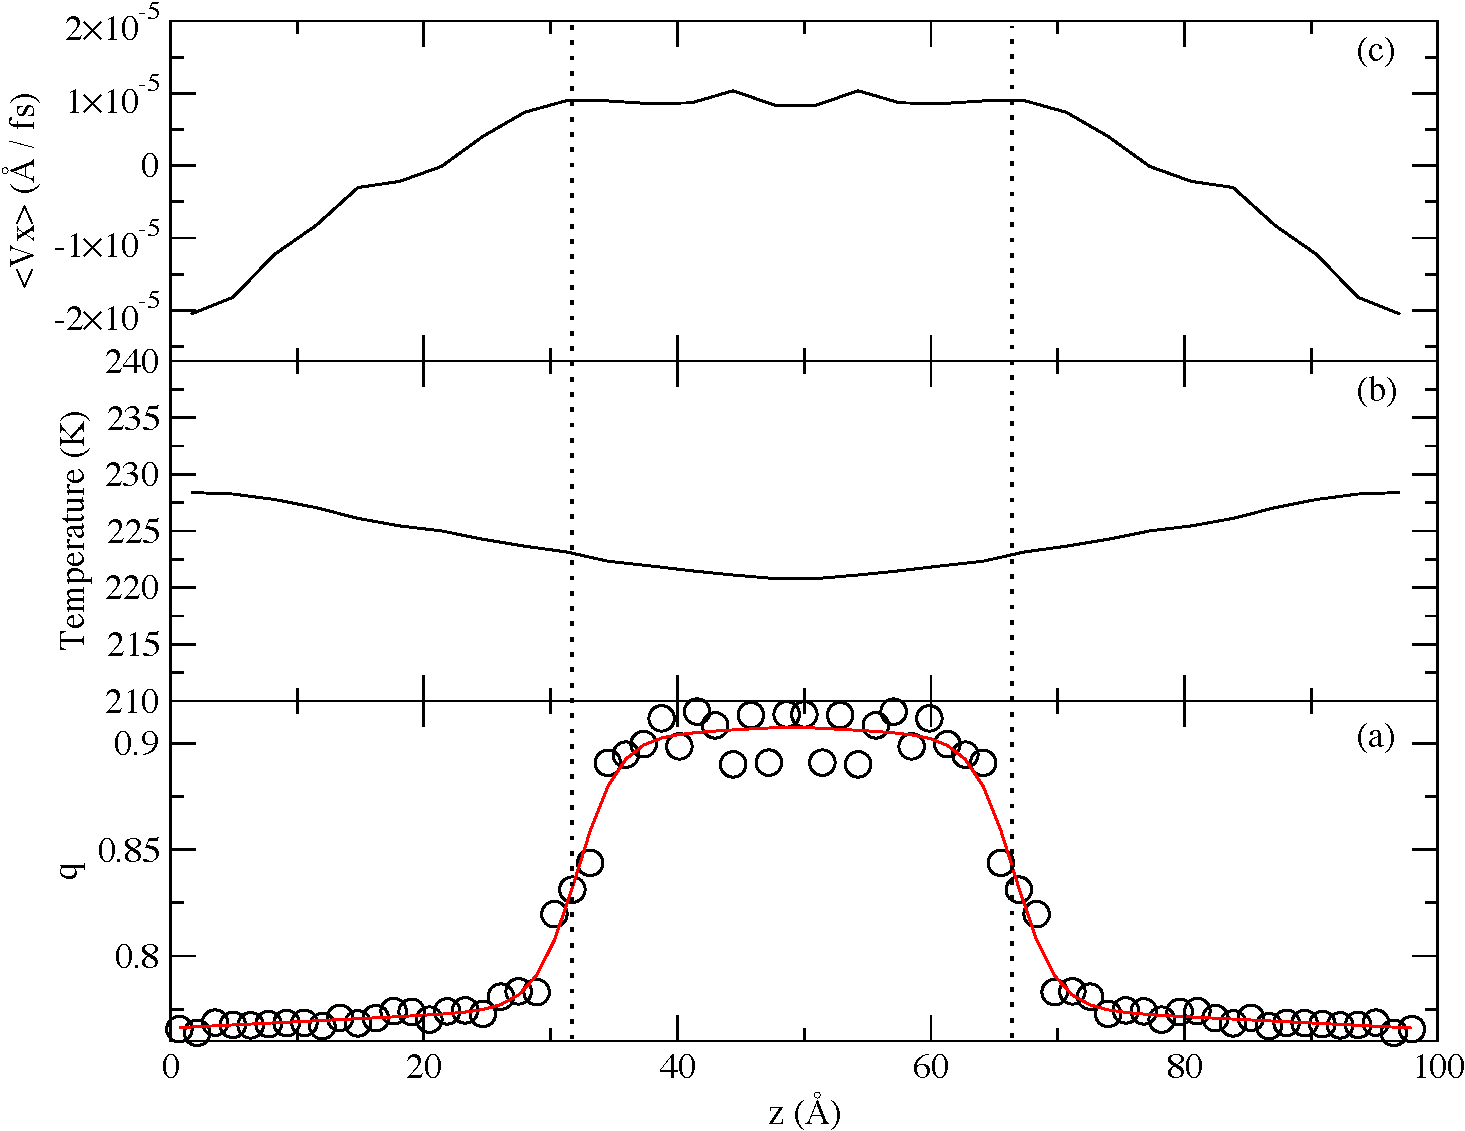
\includegraphics[width=\linewidth]{Figures/bComicStrip}
% \caption{\label{fig:bComic} The basal interface with a shear rate of
%   1.3 ms\textsuperscript{-1}.  Lower panel: the local tetrahedral order parameter, $q(z)$,
%   (black circles) and the hyperbolic tangent fit (red line).  Middle
%   panel: the imposed thermal gradient required to maintain a fixed
%   interfacial temperature.  Upper panel: the transverse velocity
%   gradient that develops in response to an imposed momentum flux.  The
%   vertical dotted lines indicate the locations of the midpoints of the
%   two interfaces.}
% \end{figure}

% \begin{figure}
% 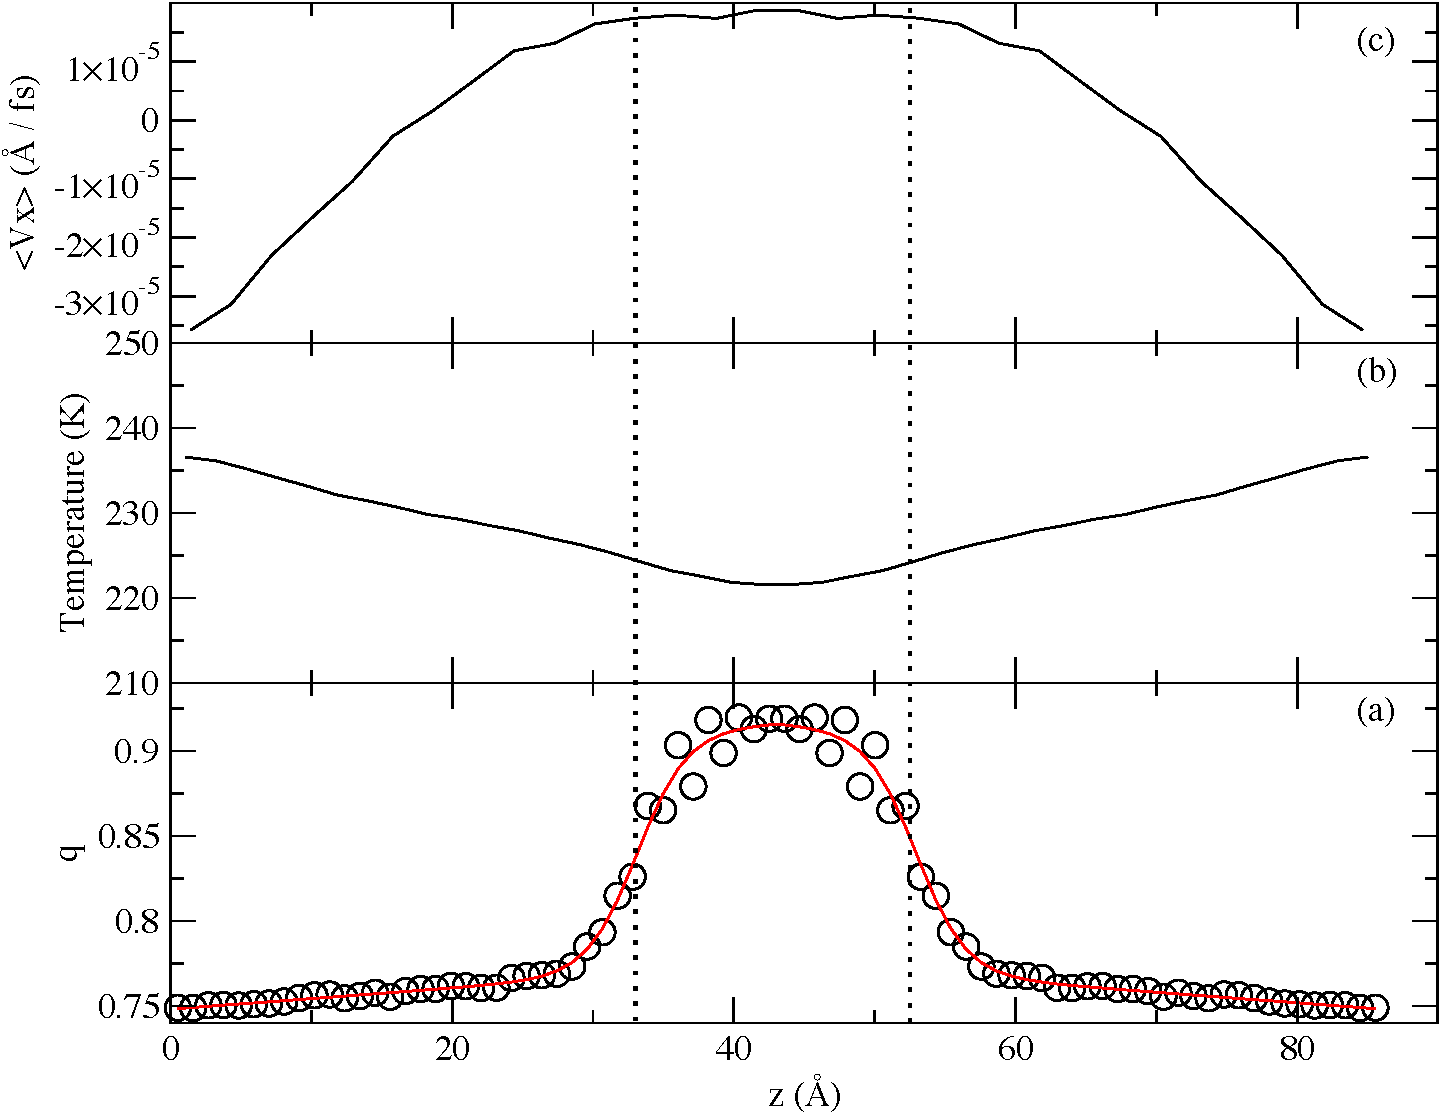
\includegraphics[width=\linewidth]{Figures/pComicStrip}
% \caption{\label{fig:pComic} The prismatic interface with a shear rate
%   of 2.0 ms\textsuperscript{-1}.  Panel
%   descriptions match those in figure \ref{fig:bComic}}
% \end{figure}

% From the fits using eq. \eqref{tet_fit}, we find the interfacial width
% for the basal and prismatic systems to be 3.2~$\pm$~0.4~\AA\ and
% 3.6~$\pm$~0.2~\AA\ , respectively, with no applied momentum flux. Over
% the range of shear rates investigated, $0.6 \pm 0.3 \mathrm{ms}^{-1}
% \rightarrow 5.3 \pm 0.5 \mathrm{ms}^{-1}$ for the basal system and
% $0.9 \pm 0.2 \mathrm{ms}^{-1} \rightarrow 4.5 \pm 0.1
% \mathrm{ms}^{-1}$ for the prismatic, we found no appreciable change in
% the interface width. The fit values for the interfacial width ($w$)
% over all shear rates contained the values reported above within their
% error bars.  Note that the interfacial widths reported here are based
% on the hyperbolic tangent parameter $w$ in Eq. \ref{tet_fit}.  This is
% related to, but not identical with, the 10\%-90\% intefacial widths
% commonly used in previous studies.\cite{Bryk02,Bryk2004b} To estimate
% the 10\%-90\% widths, it is a simple matter to scale the widths
% obtained from the hyperbolic tangent fits to obtain $w_{10-90} =
% 2.1971 \times w$.\cite{Bryk02,Bryk2004b} This results in $w_{10-90}$
% values of 7.0~$\pm$~0.9~\AA\ for the basal face, and 7.9~$\pm$~0.4
% \AA\ for the prismatic face.  These are somewhat smaller than
% previously reported values.

% \begin{figure}
% 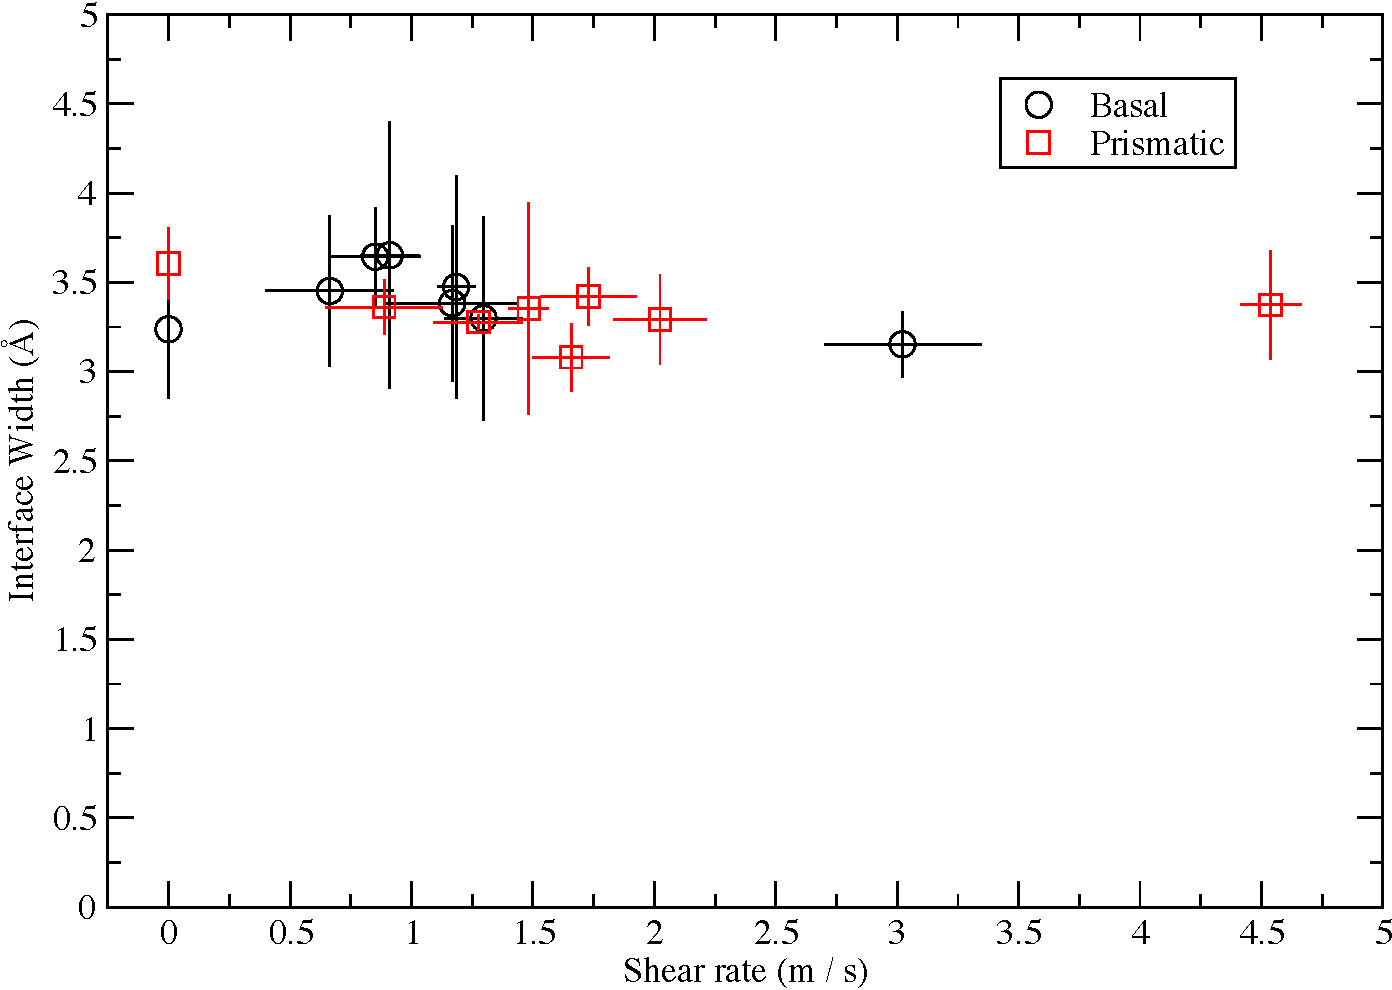
\includegraphics[width=\linewidth]{Figures/interface_width_by_shear_rate}
% \caption{\label{fig:widthByShear} The width of the ice water
%   interfaces (as measured by Eq. \ref{tet_fit}) exhibits no dependence
%   on the applied shear rate between the ice and water regions.}
% \end{figure}



% \subsubsection{Orientational Dynamics}
% The orientational time correlation function,
% \begin{equation}\label{C(t)1}
%   C_{2}(t)=\langle P_{2}(\mathbf{u}(0) \cdot \mathbf{u}(t)) \rangle,
% \end{equation}
% gives insight into the local dynamic environment around the water
% molecules.  The rate at which the function decays provides information
% about hindered motions and the timescales for relaxation.  In
% eq. \eqref{C(t)1}, $P_{2}$ is the second-order Legendre polynomial,
% the vector $\mathbf{u}$ is often taken as HOH bisector, although
% slightly different behavior can be observed when $\mathbf{u}$ is the
% vector along one of the OH bonds.  The angle brackets denote an
% ensemble average over all water molecules in a given spatial region.

% To investigate the dynamic behavior of water at the ice interfaces, we
% have computed $C_{2}(z,t)$ for molecules that are present within a
% particular slab along the $z$- axis at the initial time.  The change
% in the decay behavior as a function of the $z$ coordinate is another
% measure of the change of how the local environment changes across the
% ice/water interface.  To compute these correlation functions, each of
% the 0.5 ns simulations was followed by a shorter 200 ps microcanonical
% (NVE) simulation in which the positions and orientations of every
% molecule in the system were recorded every 0.1 ps. The systems were
% then divided into 30 bins along the $z$-axis and $C_2(t)$ was
% evaluated for each bin.

% In simulations of water at biological interfaces, Furse {\em et al.}
% fit $C_2(t)$ functions for water with triexponential
% functions,\cite{Furse08} where the three components of the decay
% correspond to a fast ($<$200 fs) reorientational piece driven by the
% restoring forces of existing hydrogen bonds, a middle (on the order of
% several ps) piece describing the large angle jumps that occur during
% the breaking and formation of new hydrogen bonds,and a slow (on the
% order of tens of ps) contribution describing the translational motion
% of the molecules.  The model for orientational decay presented
% recently by Laage and Hynes {\em et al.}\cite{Laage08,Laage11} also
% includes three similar decay constants, although two of the time
% constants are linked, and the resulting decay curve has two parameters
% governing the dynamics of decay. 

% In our ice/water interfaces, we are at substantially lower
% temperatures, and the water molecules are further perturbed by the
% presence of the ice phase nearby.  We have obtained the most
% reasonable fits using triexponential functions with three distinct
% time domains, as well as a constant piece to account for the water
% stuck in the ice phase that does not experience any long-time
% orientational decay,
% \begin{equation}
% C_{2}(t) \approx a e^{-t/\tau_\mathrm{short}} + b e^{-t/\tau_\mathrm{middle}} + c
% e^{-t/\tau_\mathrm{long}} + (1-a-b-c)
% \end{equation}
% Average values for the three decay constants (and error estimates)
% were obtained for each bin. In figures \ref{fig:basal_Tau_comic_strip}
% and \ref{fig:prismatic_Tau_comic_strip}, the three orientational decay
% times are shown as a function of distance from the center of the ice
% slab.

% \begin{figure}
% 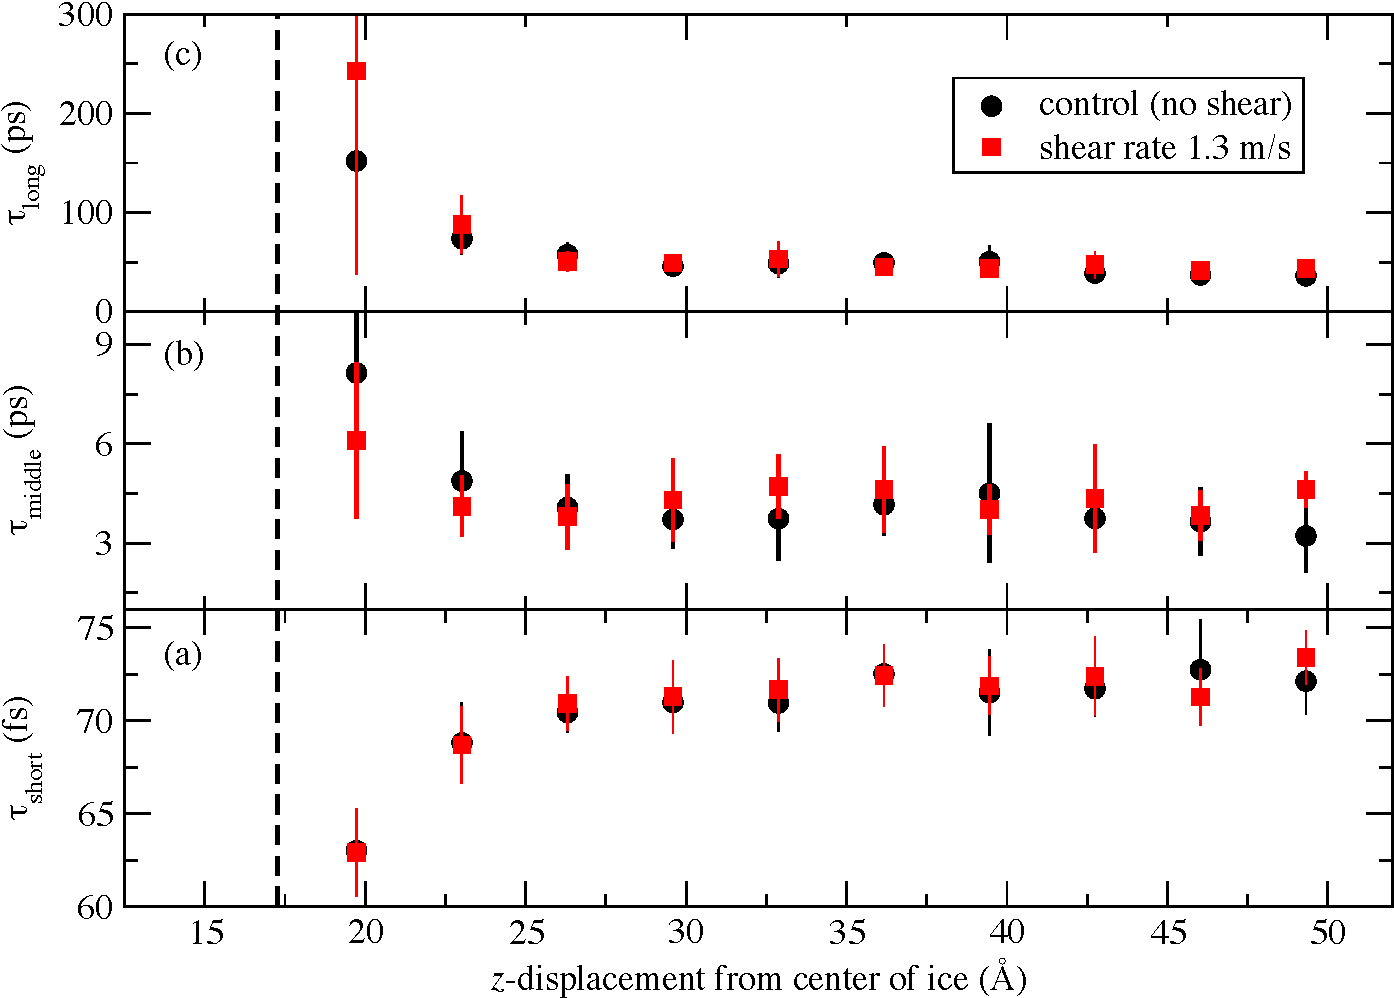
\includegraphics[width=\linewidth]{Figures/basal_Tau_comic_strip}
% \caption{\label{fig:basal_Tau_comic_strip} The three decay constants
%   of the orientational time correlation function, $C_2(t)$, for water
%   as a function of distance from the center of the ice slab.  The
%   dashed line indicates the location of the basal face (as determined
%   from the tetrahedrality order parameter) and the black and red lines
%   are fits of Eq. \ref{tauFit}.  The moderate and long
%   time contributions slow down close to the interface which would be
%   expected under reorganizations that involve large motions of the
%   molecules (e.g. frame-reorientations and jumps).  The observed
%   speed-up in the short time contribution is surprising, but appears
%   to reflect the restricted motion of librations closer to the
%   interface.}
% \end{figure}

% \begin{figure}
% 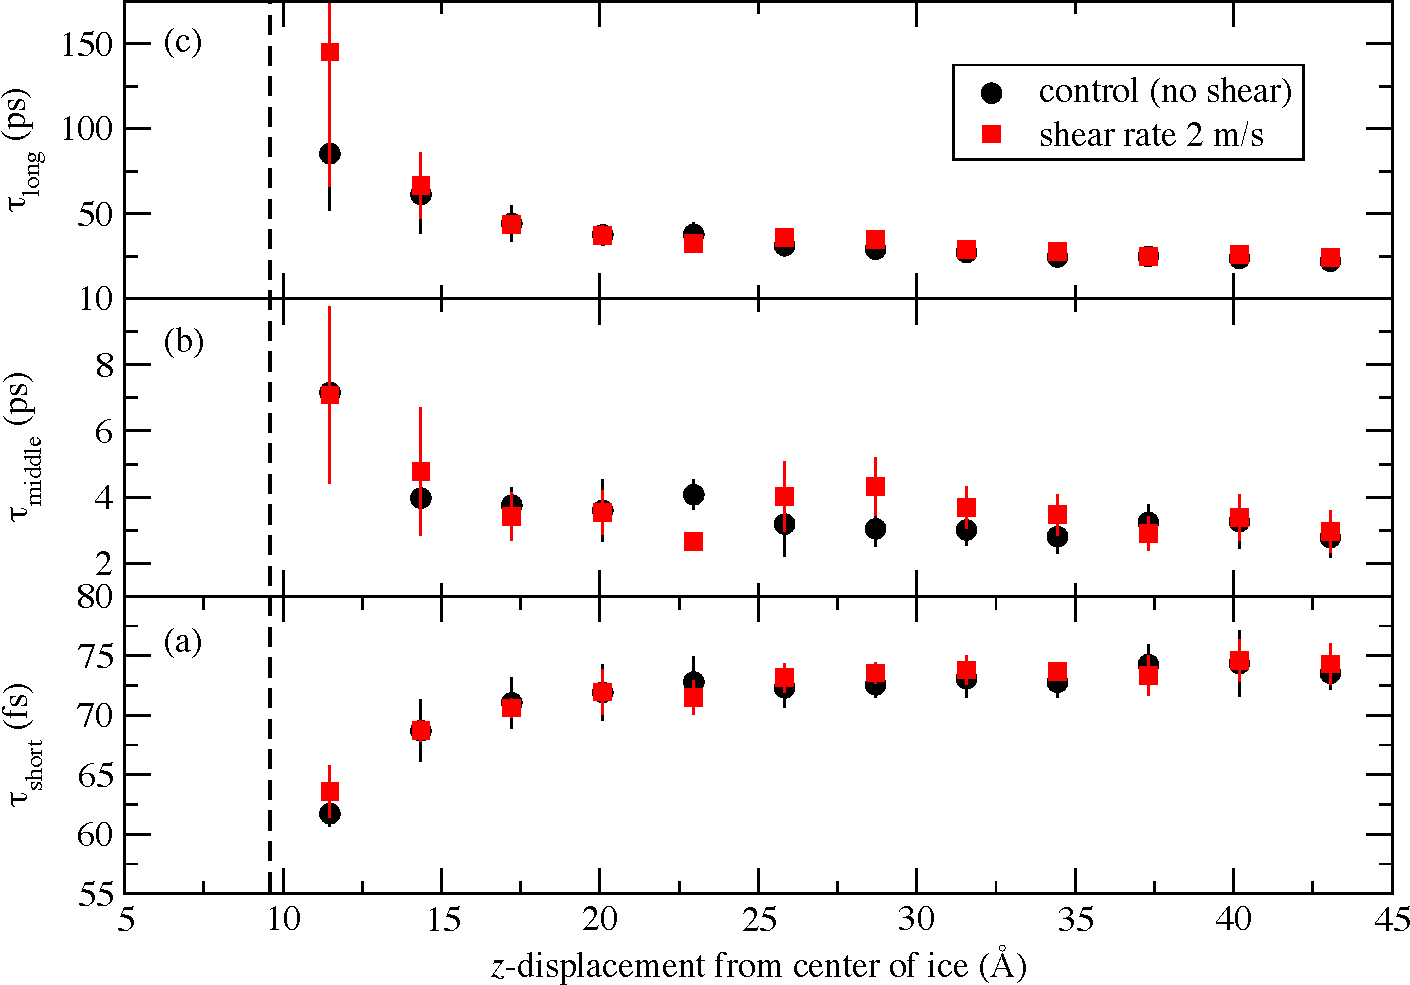
\includegraphics[width=\linewidth]{Figures/prismatic_Tau_comic_strip}
% \caption{\label{fig:prismatic_Tau_comic_strip}
%  Decay constants for $C_2(t)$ at the prismatic interface.  Panel
%   descriptions match those in figure \ref{fig:basal_Tau_comic_strip}.}
% \end{figure}

% Figures \ref{fig:basal_Tau_comic_strip} and
% \ref{fig:prismatic_Tau_comic_strip} show the three decay constants for
% the orientational time correlation function for water at varying
% displacements from the center of the ice slab for both the basal and
% prismatic interfaces.  The vertical dotted lines indicate the
% locations of the midpoints of the interfaces as determined by the
% tetrahedrality fits. In the liquid regions, $\tau_{middle}$ and
% $\tau_{long}$ have consistent values around 3-4 ps and 20-40 ps,
% respectively, and increase in value approaching the interface.
% According to the jump model of Laage and Hynes {\em et
%   al.},\cite{Laage08,Laage11} $\tau_{middle}$ corresponds to the
% breaking and making of hydrogen bonds and $\tau_{long}$ is explained
% with translational motion of the molecules (i.e. frame reorientation).
% The shortest of the three decay constants, the librational time
% $\tau_\mathrm{short}$ has a value of about 70 fs in the liquid region,
% and decreases in value approaching the interface. The observed
% speed-up in the short time contribution is surprising, but appears to
% reflect the restricted motion of librations closer to the interface.

% The control systems (with no applied momentum flux) are shown with
% black symbols in figs. \ref{fig:basal_Tau_comic_strip} and
% \ref{fig:prismatic_Tau_comic_strip}, while those obtained while a
% shear was active are shown in red.

% Two notable features deserve clarification.  First, there are
% nearly-constant liquid-state values for $\tau_{short}$,
% $\tau_{middle}$, and $\tau_{long}$ at large displacements from the
% interface. Second, there appears to be a single distance, $d_{basal}$
% or $d_{prismatic}$, from the interface at which all three decay times
% begin to deviate from their bulk liquid values. To quantify this
% distance, each of the decay constant $z$-profiles were fit to
% \begin{equation}\label{tauFit}
% \tau(z)\approx\tau_{liquid}+(\tau_{solid}-\tau_{liquid})e^{-(z-z_{wall})/d}
% \end{equation}
% where $\tau_{liquid}$ and $\tau_{solid}$ are the liquid and projected
% solid values of the decay constants, $z_{wall}$ is the location of the
% interface, and $d$ is the displacement the deviations occur at (see
% Figures \ref{fig:basal_Tau_comic_strip} and
% \ref{fig:prismatic_Tau_comic_strip}). The displacements $d_{basal}$
% and $d_{prismatic}$ were determined for each of the three decay
% constants, and then averaged for better statistics.
% For the basal system, we found $d_{basal}$ for the control set to be
% 2.9 \AA\, and 2.8 \AA\ for a simulation with a shear rate of 1.3
% ms\textsuperscript{-1}. We found $d_{prismatic}$ to be slightly
% larger than $d_{basal}$ for both the control and an applied shear,
% with displacements of 3.6 \AA\ for the control system and 3.5 \AA\ for
% a simulation with a 2 ms\textsuperscript{-1} shear rate. From this we
% can conclude there is no apparent dependence on the shear rate for the dynamic interface
% width. 

% %%%%%%%%Should we keep this paragraph???%%%%%%%%%%%%%%%
% Beaglehole and Wilson have measured the ice/water interface using
% ellipsometry and find a thickness of approximately 10~\AA\ for both
% the basal and prismatic faces.\cite{Beaglehole93} Structurally, we
% have found the basal and prismatic interfacial width to be
% 3.2~$\pm$~0.4~\AA\ and 3.6~$\pm$~0.2~\AA.  Decomposition of
% the spatial dependence of the decay times of $C_2(t)$ shows good
% agreement with the structural interfacial width determined by the
% local tetrahedrality.
% %%%%%%%%%%%%%%%%%%%%%%%%%%%%%%%%%%%%%%%%%%%%%%


% \subsection{Coefficient of Friction of the Interface}
% As liquid water flows over an ice interface, there is a distance from
% the structural interface where bulk-like hydrodynamics are recovered.
% Bocquet and Barrat constructed a theory for the hydrodynamic boundary
% parameters, which include the slipping length
% $\left(\delta_\mathrm{wall}\right)$ of this boundary layer and the
% ``hydrodynamic position'' of the boundary
% $\left(z_\mathrm{wall}\right)$.\cite{PhysRevLett.70.2726,PhysRevE.49.3079}
% This last parameter is the location (relative to a solid surface)
% where the bulk-like behavior is recovered.  Work by Mundy {\it et al.}
% has helped to combine these parameters into a liquid-solid friction
% coefficient, which quantifies the resistance to pulling the solid
% interface through a liquid,\cite{Mundy1997305}
% \begin{equation}
% \lambda_\mathrm{wall} = \frac{\eta}{\delta_\mathrm{wall}}.
% \end{equation}
% This expression is nearly identical to one provided by Pit {\it et
%   al.} for the solid-liquid friction of an interface,\cite{Pit99}
% \begin{equation}\label{Pit}
%   \lambda=\frac{\eta}{\delta}
% \end{equation}
% where $\delta$ is the slip length for the liquid measured at the
% location of the interface itself.  In our simulations, the shoulder on
% the velocity profile indicating the location of the hydrodynamic
% boundary in the liquid is not always apparent. In some cases, the
% linear behavior persists nearly up to the interfacial region.  For
% this reason, the hydrodynamic position of the boundary is not always
% computable, while the Pit approach (Eq. \ref{Pit}) can be used to find
% the solid-liquid friction coefficient more reliably.

% In both the Pit and hydrodynamic boundary expressions, $\eta$ is the
% shear viscosity of the bulk-like region of the liquid, a quantity
% which is easily obtained in VSS-RNEMD simulations by fitting the
% velocity profile in the region far from the surface.\cite{Kuang12}
% Assuming linear response in the bulk-like region,
% \begin{equation}\label{Kuang}
% j_{z}(p_{x})=-\eta \left(\frac{\partial v_{x}}{\partial z}\right)
% \end{equation}
% Substituting this result into eq. \eqref{Pit}, we can estimate the
% solid-liquid coefficient using the slip length,
% \begin{equation}
% \lambda=-\frac{j_{z}(p_{x})} {\left(\frac{\partial v_{x}}{\partial
%       z}\right) \delta}
% \end{equation}

% For ice / water interfaces, the boundary conditions are no-slip, so
% projecting the bulk liquid state velocity profile yields a negative
% slip length. This length is the difference between the structural edge
% of the ice (determined by the tetrahedrality profile) and the location
% where the projected velocity of the bulk liquid intersects the solid
% phase velocity (see Figure \ref{fig:delta_example}). The coefficients
% of friction for the basal and the prismatic facets were determined for
% shearing along both the $x$ and $y$ axes.  The values are given in
% table \ref{tab:lambda}. 

% Note that the measured friction coefficient for the basal face is
% twice that of the prismatic face (regardless of drag direction).
% These results may seem surprising as the basalface appears smoother
% than the prismatic with only small undulations of the oxygen
% positions, while the prismatic surface has deep corrugated channels
% along the $x$ direction in the crystal system used in this work.
% However, the corrugations are relatively thin, and the liquid phase
% water does not appear to populate the channels.  The prismatic face
% therefore effectively presents stripes of solid-phase molecules
% (making up approximately half of the exposed surface area) with nearly
% empty space between them. The interfacial friction appears to be
% independent of the drag direction, so flow parallel to these channels
% does not explain the lower friction of the prismatic face.  A more
% likely explanation is that the effective contact between the liquid
% phase and the prismatic face is reduced by the empty corrugations.  

% \begin{figure}
% 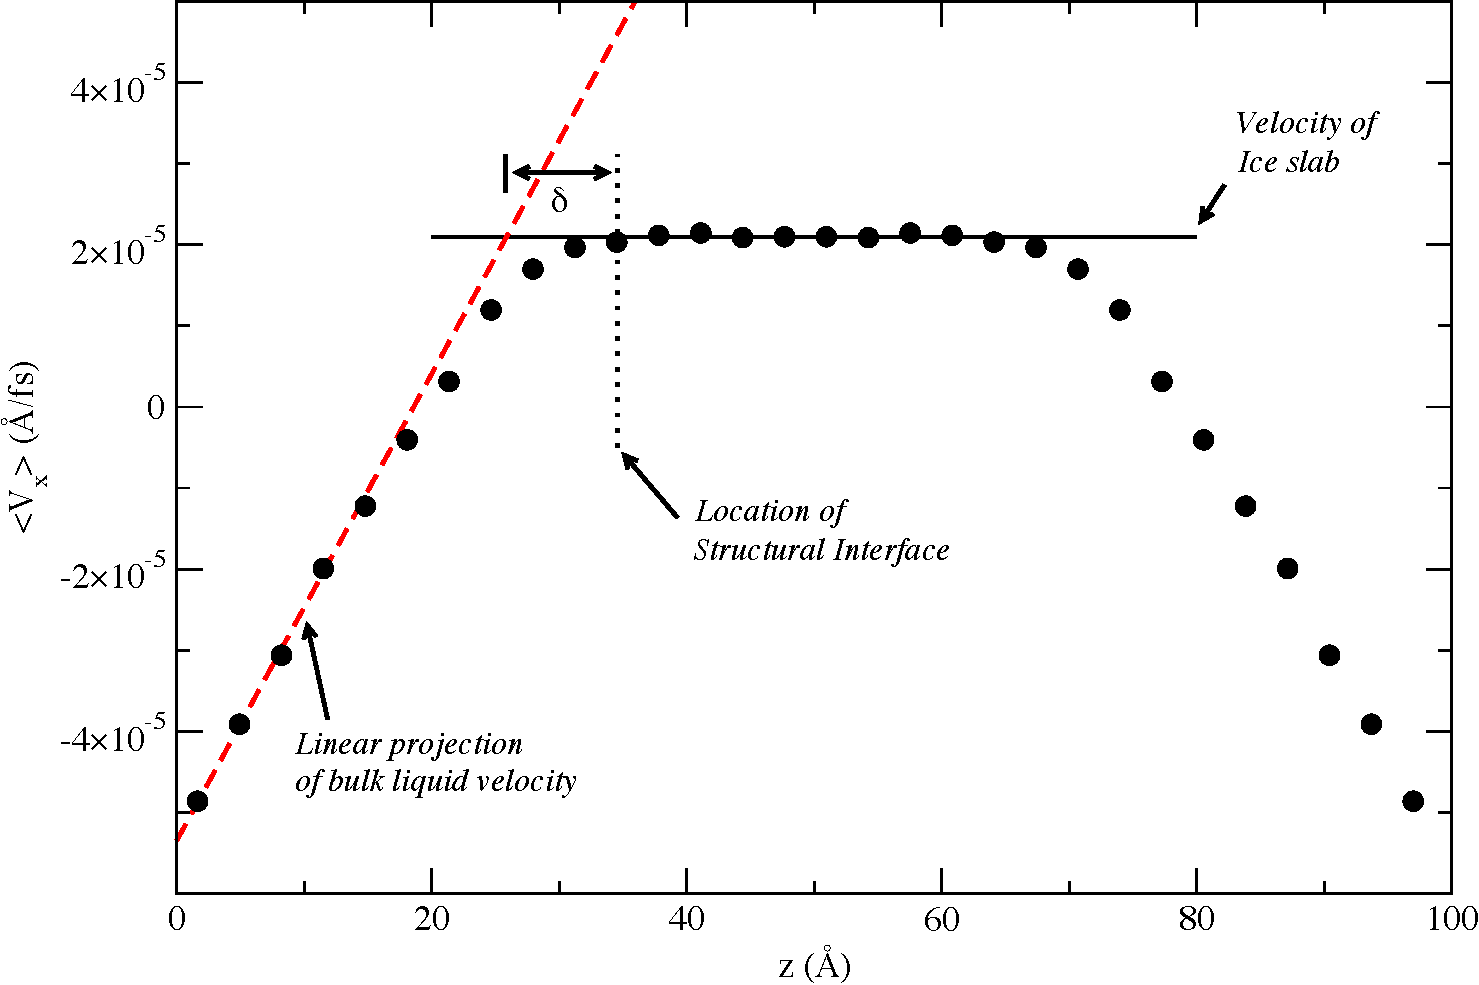
\includegraphics[width=\linewidth]{Figures/delta_example}
% \caption{\label{fig:delta_example} Determining the (negative) slip
%   length ($\delta$) for the ice-water interfaces (which have decidedly
%   non-slip behavior).  This length is the difference between the
%   structural edge of the ice (determined by the tetrahedrality
%   profile) and the location where the projected velocity of the bulk
%   liquid (dashed red line) intersects the solid phase velocity (solid
%   black line).  The dotted line indicates the location of the ice as
%   determined by the tetrahedrality profile.  This example is taken
%   from the basal-face simulation with an applied shear rate of 3.0 ms\textsuperscript{-1}.}
% \end{figure}


% \begin{table}[h]
% \centering
% \caption{Solid-liquid friction coefficients (measured in amu~fs\textsuperscript{-1}) }
% \label{tab:lambda}
% \begin{tabular}{|ccc|}  \hline
%            & \multicolumn{2}{c|}{Drag direction} \\ 
%  Interface & $x$               & $y$  \\ \hline
%      basal &  $0.08 \pm 0.02$  & $0.09 \pm 0.03$ \\
%  prismatic & $0.037 \pm 0.008$ & $0.04 \pm 0.01$ \\ \hline
% \end{tabular}
% \end{table}


% \section{Conclusion}
% We have simulated the basal and prismatic facets of an SPC/E model of
% the ice I$_\mathrm{h}$ / water interface.  Using VSS-RNEMD, the ice
% was sheared relative to the liquid while simultaneously being exposed
% to a weak thermal gradient which kept the interface at a stable
% temperature.  Calculation of the local tetrahedrality order parameter
% has shown an apparent independence of the interfacial width on the
% shear rate.  This width was found to be 3.2~$\pm$0.4~\AA\ and
% 3.6~$\pm$0.2~\AA\ for the basal and prismatic systems, respectively.

% Orientational time correlation functions were calculated at varying
% displacements from the interface, and were found to be similarly
% independent of the applied momentum flux. The short decay due to the
% restoring forces of existing hydrogen bonds decreased close to the
% interface, while the longer-time decay constants increased in close
% proximity to the interface.  There is also an apparent dynamic
% interface width, $d_{basal}$ and $d_{prismatic}$, at which these
% deviations from bulk liquid values begin.  We found $d_{basal}$ and
% $d_{prismatic}$ to be approximately 2.8~\AA\ and 3.5~\AA\ . This
% interfacial width is in good agreement with values determined by the
% structural analysis of the interface, by the hyperbolic tangent fit of
% the local tetrahedral order parameter.

% The coefficient of liquid-solid friction for each of the facets was
% also determined. They were found to be
% 0.07~$\pm$~0.01~amu~fs\textsuperscript{-1} and
% 0.032~$\pm$~0.007~amu~fs\textsuperscript{-1} for the basal and
% prismatic facets respectively. We attribute the large difference
% between the two friction coefficients to the direction of the shear
% and to the surface structure of the crystal facets.




%%%%%%%%%%%%%%%%%%%%%%%%%%%%%%%%%%%%%%%%%%%%%%%%%%%%%%%%%%%%%%%%%%%%%%%%%%%%%%%%%%%
%		CHAPTER 3 -- Structural Width of Ice / Water Interfaces
%%%%%%%%%%%%%%%%%%%%%%%%%%%%%%%%%%%%%%%%%%%%%%%%%%%%%%%%%%%%%%%%%%%%%%%%%%%%%%%%%%%
% To add:
% 1. Density section, fits, values, widths, etc.
% 2. interfacial width by shear rate plot for tetrahedrality
% 3. interfacial width by shear rate plot for density?

\chapter{STRUCTURAL WIDTHS OF ICE-I$_\mathrm{h}$ / WATER
  INTERFACES}\label{chap:Str}


\begin{flushright}
\textit{''Why do snowflakes always fall as flat structures with six corners?''} \\
-Joannes Kepler (1611) \\
\end{flushright}

One of the open questions about ice / water interfaces is whether the
thickness of the interfacial `slush' layer depends on the facet of ice
presented to the water. In the interfacial region, the water molecules
are ordered differently than in either the solid or liquid phases, and
also exhibit dynamics unique to their local structure.  The width of
this interfacial layer has been estimated by finding the distance over
which structural order parameters or dynamic properties change from
their bulk liquid values to those of the solid ice. The properties
used to find interfacial widths have included the local density, the
diffusion constant, and both translational and orientational order
parameters~\cite{Karim1988,Karim1990,Hayward2001,Hayward2002,Bryk2002,Gay2002,Louden2013a}. Throughout
shearing simulations, the VSS-RNEMD method employed here creates
thermal and velocity gradients in the system, during which the momenta
of the water molecules are perturbed. Due to this, any order parameters that
depends on translational motion may measure the momentum exchange and
not physical properties of the interface. To avoid these influences,
we have probed the ice-I$_\mathrm{h}$ / water interface under shear by
observing the transition of several order parameters independent of
momenta from their ice to bulk liquid values.  In this chapter, we
focus on structural order parameters for measurements of interfacial
width, and consider dynamic order parameters in Chapter
\ref{chap:Dyn}.

\section{Density Measurements Transverse to the Interface}
One of the many anomolies of water is that under ambient conditions
the density of the solid is less than that of the liquid. The
tetrahedral structure of ice-I$_\mathrm{h}$ is more open than the
local solvation environment of the liquid, which gives rise to this
phenomena. Liquid water at the surface of ice would experience two
different environments on either side of the molecule; ice-like
templating from the exposed solid and liquid-like packing on the
other. Due to this, the liquid may take on a configuration that is
unique to its local environment, and this deviation from bulk
liquid-like structures may take several molecular layers to dampen
out. Therefore it may be possible to quantify the transition between
the solid and the bulk liquid by observing the length scale over which
these effects diminish.

In order to understand what affect shearing has on the structure of
water at the ice-I$_\mathrm{h}$ / water interface, we initially
studied the systems without imposed thermal or momentum
fluxes. Following the pioneering work of Haymet \textit{et al.}, we
probed the interface by examining the transition of the density of
molecules from bulk liquid to bulk
ice.\cite{Karim1987,Karim1990,Hayward2001,Bryk2004} Four consecutive 1
ns simulations of quiescent ice / water systems were performed for
each exposed crystal face. These simulations were performed under a
constant volume and constant energy integrator (NVE), equilibrated at
the coexistence temperature (225~K for SPC/E and 270~K for
TIP4P/Ice). During the simulations, the positions of the water
molecules were sampled every 0.1 ps.

To compute transverse density profiles, each frame of the trajectories
were divided into 0.25~\AA~bins, and the average density of each bin
was accumulated. The density profiles were then fit with a hyperbolic
tangent function designed to smoothly transition between the bulk
liquid and ice domains. Following Haymet \textit{et al.}, only the
density maximas corresponding to the planes of ice were included in
the data in the ice regions.
\begin{equation}\label{rho_fit}
\rho (z) \approx
\rho_\mathrm{liq}+\frac{\rho_\mathrm{ice}-\rho_\mathrm{liq}}{2}\left[\tanh\left(\frac{z-l}{w^\rho}\right)-\tanh\left(\frac{z-r}{w^\rho}\right)\right]
\end{equation}
Here, $\rho_\mathrm{liq}$ and $\rho_\mathrm{ice}$ are the densities of
the liquid and ice respectively. The $z$-locations of the left and
right Gibbs dividing surfaces are $l$ and $r$, and $w^\rho$ is the
width of the interface. An example density profile for each of the
SPC/E interfaces is shown in Figure \ref{fig:transDensity} (a similar
set of graphs for the TIP4P-Ice modeled systems can be seen in Figure
\ref{fig:TIPtransDensity} in Appendix \ref{structAppendix}).

\begin{figure*}
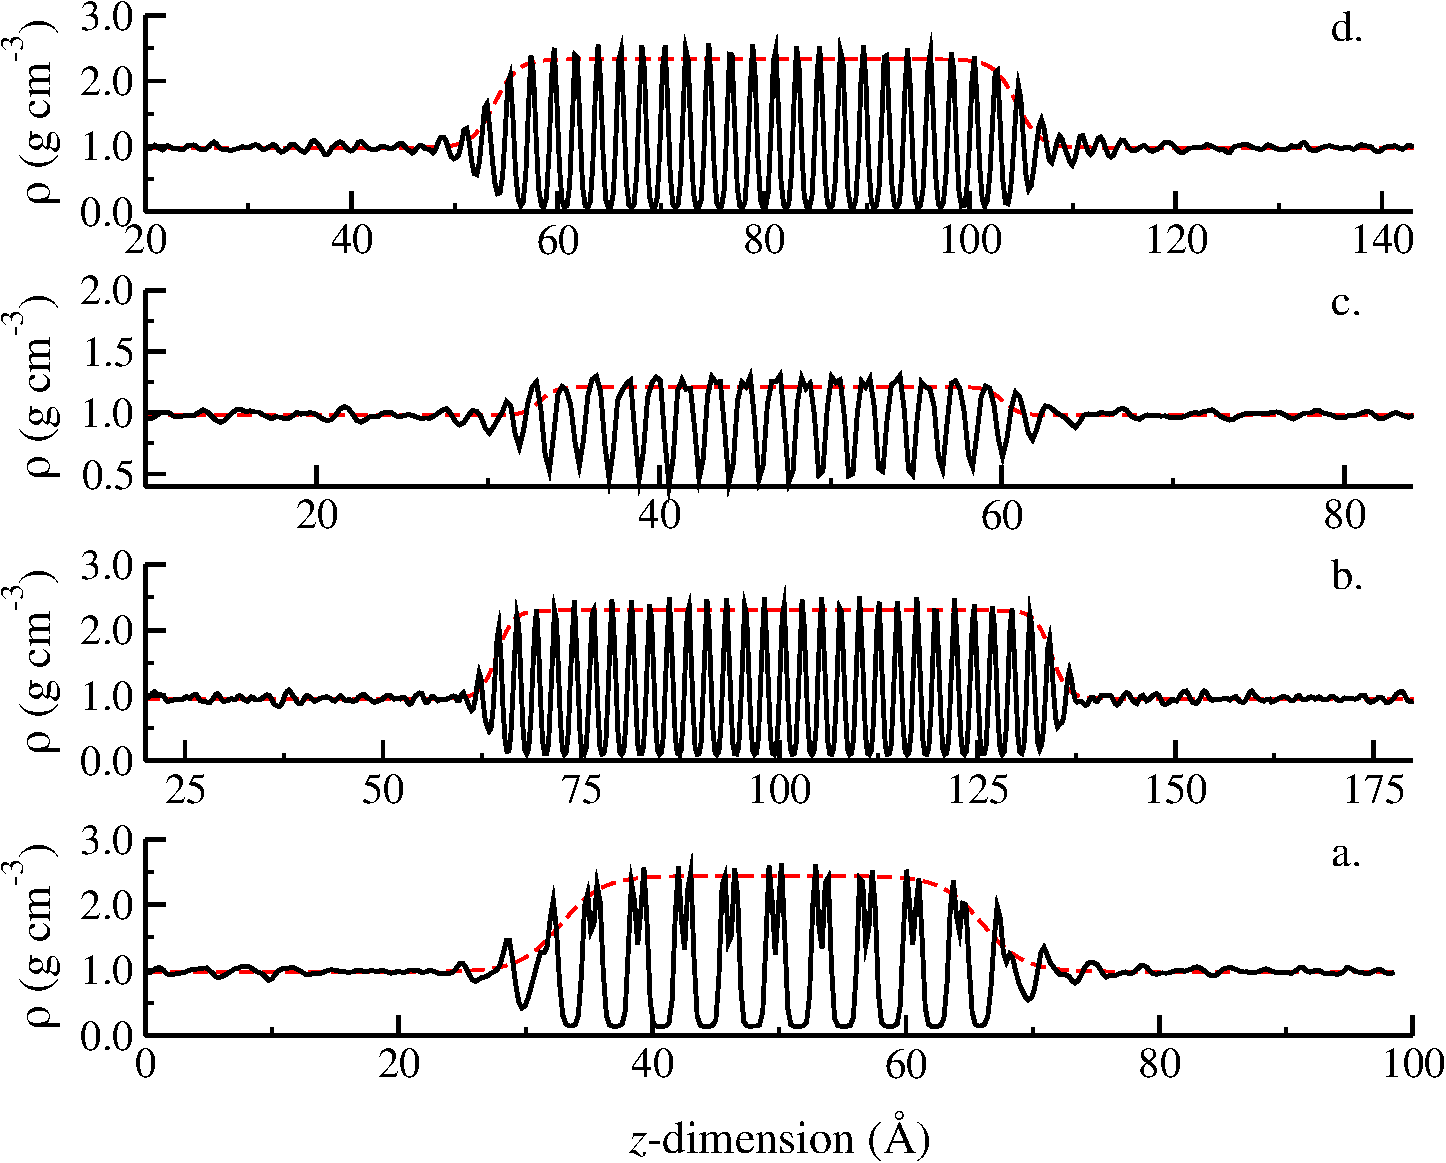
\includegraphics[width=\linewidth]{Figures/transDensity}
\caption{\label{fig:transDensity}Transverse density profiles for the
  basal (a), prismatic (b), 14\degree~pyramidal (c) and secondary prism (d)
  facets of an SPC/E ice-I$_\mathrm{h}$ / water interface (black
  lines). The prismatic and secondary prism profiles are zoomed in to
  show detail at the ice / water interface. The profiles are fit using
  Equation \eqref{rho_fit} (dashed red lines).}
\end{figure*}

From Equation \eqref{rho_fit}, we have obtained estimates for
$w^{\rho}$; these values are related to the $10\%-90\%$ interfacial
widths commonly reported in previous studies
($w_\mathrm{10-90}^{\rho} = 2.197~w^{\rho}$).\cite{Bryk2002,Bryk2004}
The results for the SPC/E and TIP4P/Ice interfaces are reported in
Table \ref{tab:strWidths}.

\begin{table}[h]
\centering
\caption{COMPUTED WIDTHS OF THE ICE-I$_\mathrm{h}$ / WATER INTERFACES BY
  STRUCTURAL MEASURES \label{tab:strWidths}} 
\begin{tabular}{r|cc|cc}  
\hline
\hline
  \multirow{2}{*} & \multicolumn{2}{c|}{SPC/E (225~K)} &  \multicolumn{2}{c}{TIP4P/Ice (270~K) } \\
  & \multicolumn{2}{c|} {Interfacial Widths (\AA)} &
                                                                      \multicolumn{2}{c} {Interfacial Widths  (\AA)} \\
 Interface &  $w_\mathrm{10-90}^{\rho}$ & $w_\mathrm{10-90}^{q}$ &  $w_\mathrm{10-90}^{\rho}$ &  $w_\mathrm{10-90}^{q}$ \\ 
\hline
  Basal  $\{0001\}$                 & 9(1) & 7.5(4) & 11(1) & 8.8(8)  \\
  Prismatic  $\{10\bar{1}0\}$       & 7(2)  & 7.2(2) & 9(1) & 9.0(5)  \\
  14\degree~Pyramidal  $\{20\bar{2}1\}$       & 3.1(6) & 6.6(2) & 3.7(6) & 8.2(5)  \\
  Secondary Prism  $\{11\bar{2}0\}$ & 8(1) &6.7(2) & 11.2(2) & 9.4(6)  \\ 
\hline
\hline
\end{tabular}
\flushleft
 Uncertainties in the last digit are indicated with parentheses. \\
\end{table}

For the SPC/E basal, prismatic, and secondary prism interfaces, we
estimate an interfacial width $w_\mathrm{10-90}^{\rho} \sim$ 8
\AA~. However, the solid to liquid density transition for the
14\degree~pyramidal interface is observed to occur over $\sim$ 3
\AA~. This result suggests the transition from ice to liquid water
occurs over a single molecular diameter for the pyramidal interface,
while over several molecular diameters for the other ice facets. Since
the 14\degree~pyramidal crystal does not have well defined
crystallographic planes perpendicular to the dimension normal to the
surface, fitting the resulting density profiles gives potentially
skewed results. A similar trend is observed in the TIP4P/Ice estimates
of $w_\mathrm{10-90}^{\rho}$. The basal and two prismatic interfaces
are found to be of similar width, although slightly broader than those
predicted by SPC/E. This can be attributed to the warmer coexistence
temperature of the TIP4P/Ice model. However, the pyramidal width
appears to suffer from the same issue as in the SPC/E fits.  Since the
density profiles (black lines) require subjective fitting (red
dashed-lines) and the resulting estimates of the interfacial widths
using this metric are faulty for certain orientations of the crystal,
it is desirable to consider a second structural order parameter for
comparison.

\section{Local Tetrahedral Order Parameter}\label{sec:tetra}
As a second structural measure of the interface, we have used the
local tetrahedral order parameter, which compares the local molecular
environments (e.g. the angles between nearest neighbor molecules) to
perfect tetrahedral ordering. This method would not be skewed due to
rotations of the crystal, and would therefore more accurately quantify
the transition of the local structure through the interface. This
quantity was originally described by Chau and
Hardwick,~\cite{Chau1998} was rescaled by Errington and
Debenedetti,~\cite{Errington2001} and has been used in bulk liquid
simulations by Kumar \textit{et al.}~\cite{Kumar2009}, and at ice /
water interfaces by Bryk and Haymet~\cite{Bryk2004}.

We have evaluated the local tetrahedral order parameter, $q$, along
the coordinate perpendicular to the ice / water interface,
\textit{i.e}., the $z$-axis of the simulation box. With $N$ total molecules,
\begin{equation}
q(z) = \frac{1}{N_z} \int_0^L \sum_{i=1}^{N} \Bigg(1 -\frac{9}{2n(n-1)}\sum_{j=1}^{n-1}
\sum_{k=j+1}^{n} \bigg(\cos\psi_{jik}+\frac{1}{3}\bigg)^2\Bigg)
\delta(z_{i}-z)\mathrm{d}z .
\label{eq:qz}
\end{equation}
$\psi_{jik}$ is the angle formed between the oxygen sites of water
molecules $i$, $j$, and $k$, where molecule $i$ is the central water
molecule (with $n$ neighbors) and molecules $j$ and $k$ are two of the
neighbors of $i$.  The neighboring molecules $j$ and $k$ are
restricted to lie within the first solvation shell of molecule $i$
($r < 3.41$~\AA\ for water), and the double sum visits all angles for
the $n$ neighbors of molecule $i$ that are within this distance.  When
molecule $i$ has exactly four neighbors ($n=4$), the prefactor reduces
to $3/8$, as in the expression of Errington and Debenedetti, but
Equation \eqref{eq:qz} also provides tetrahedrality information for water
molecules that are either under- or over-coordinated. We have also
introduced the normalization factor
$N_z = \sum_i \int \delta(z_i - z) \mathrm{d}z$ to account for the
varying populations of water molecules within each finite-width bin.

At low temperatures, the tetrahedral order parameter can approach
unity for perfect ice-I$_\mathrm{h}$ structures. However, at
temperatures close to melting, values of 0.9 are more common in SPC/E
ice due to thermal motion in the lattice. In the liquid, overlap of
the local environment with a perfect tetrahedron is reduced, and
values of $q(z) \approx 0.75$ are common in SPC/E water at 225~K. The
results indicate more tetrahedral structure in TIP4P/Ice; at
270~K, tetrahedrality averages, $q(z) \approx 0.95$ and $0.75$ are
found in the ice and liquid, respectively.

The structural widths of the ice-I$_\mathrm{h}$ / water interfaces
were determined by dividing each system into 1~\AA~ bins along the
$z$-axis, and computing statistical averages of $q(z)$ in each
bin. For the secondary prism interface (using SPC/E water at 225~K),
the resulting distribution can be seen in the bottom panel of
Figure \ref{fig:spComic} and for comparison, Figure \ref{fig:tipsComic}
shows the same interface using the TIP4P/Ice model at 270~K.  (See
Appendix \ref{structAppendix} for the other interfaces with the SPC/E
and TIP4P/Ice models). In the bulk liquid (at small and large values
of $z$) of Figure \ref{fig:spComic}, the order parameter takes on values
of $q(z) \approx~0.77$, while $q(z) \approx~0.92$~was found in bins
spanning the ice. The tetrahedrality profiles were fit using the same
functional form as the density profiles, however, an additive term was
included to account for the change in tetrahedral ordering due to the
thermal gradient throughout the system for simulations where thermal
fluxes were applied (turquoise line in the bottom panel of the same
figures),
\begin{equation}\label{tet_fit}
q(z) \approx
q_\mathrm{liq}+\frac{q_\mathrm{ice}-q_\mathrm{liq}}{2}\left[\tanh\left(\frac{z-l}{w^q}\right)-\tanh\left(\frac{z-r}{w^q}\right)\right]+\beta\left|z-\frac{r+l}{2}\right|.
\end{equation}
Here $q_\mathrm{liq}$ and $q_\mathrm{ice}$ are the values of the order
parameter for the bulk liquid and ice domains. The locations $l$ and
$r$ are the $z-$coordinates of the Gibbs dividing surface for the left
and right interfaces (shown in Figure \ref{fig:spComic} with vertical
dotted lines), and $w^{q}$ is the interfacial width.  The last term in
Equation \eqref{tet_fit} accounts for the influence of the weak thermal
gradient on the tetrahedrality profile in the liquid region. Namely,
at warmer temperatures the liquid is able to adopt local
configurations resulting in lower values of the order parameter. This
results in a small linear decay in the tetrahedrality profiles for
increasing displacements from the ice surface.

\begin{figure*}
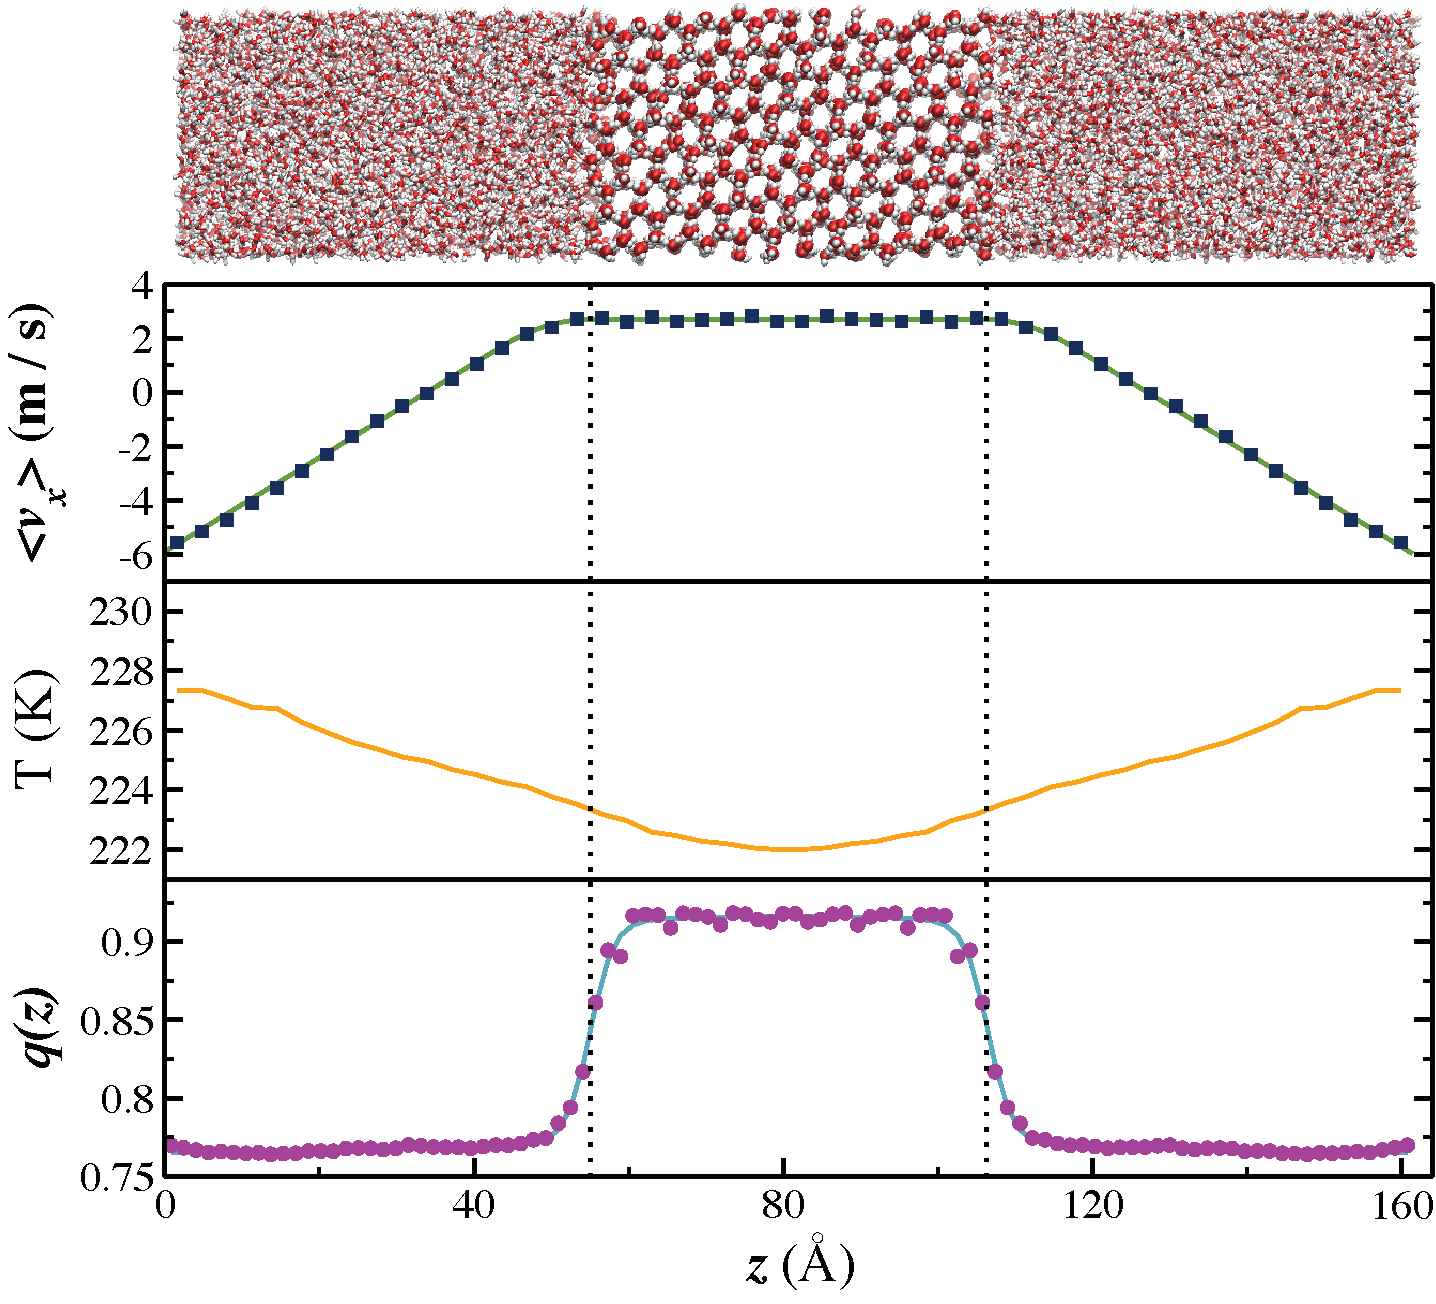
\includegraphics[width=\linewidth]{Figures/SecPrismComicStrip}
\caption{\label{fig:spComic} Properties of the SPC/E secondary prism
  interface (top) being sheared through water at 8.6 m
  s\textsuperscript{-1}. Lower panel: the local tetrahedral order
  parameter, $q(z)$, (circles) and the hyperbolic tangent fit
  (turquoise line).  Middle panel: the imposed thermal gradient
  required to maintain a fixed interfacial temperature of $\sim$225 K
  with the SPC/E water model. Upper panel: the transverse velocity
  gradient (squares) that develops in response to an imposed momentum
  flux, along with the fit (green line). The vertical dotted lines
  indicate the locations of the Gibbs dividing surfaces of the two
  interfaces.}
\end{figure*}


\begin{figure*}
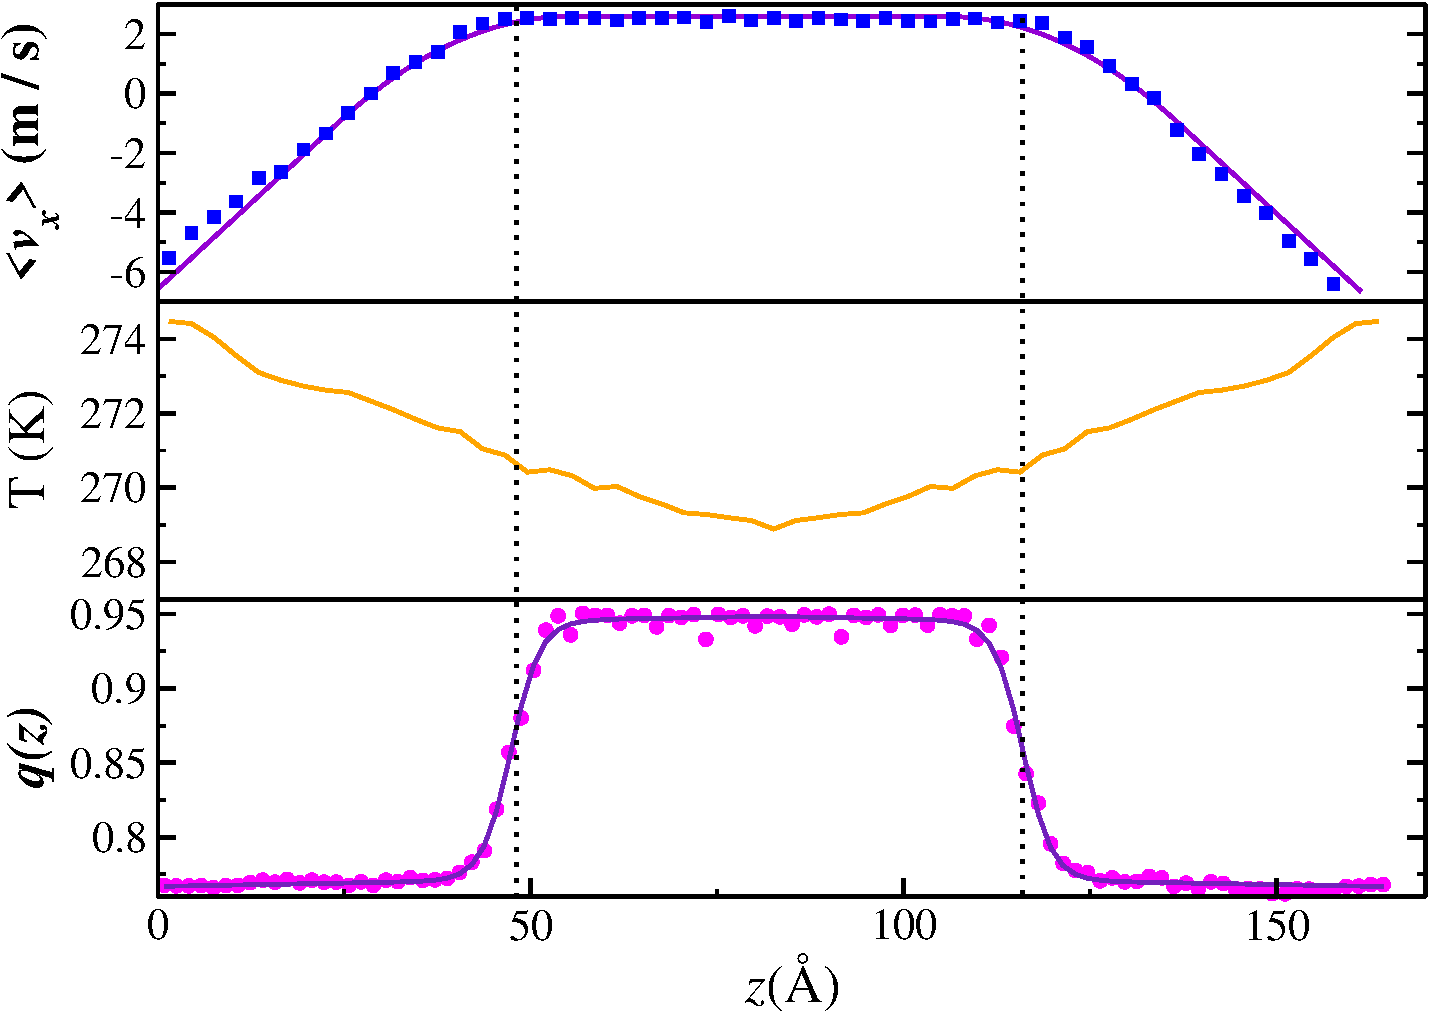
\includegraphics[width=\linewidth]{Figures/SecPrism_TIP4PIce_Plot}
\caption{\label{fig:tipsComic} Properties of the TIP4P/Ice secondary prism
  interface being sheared through water at 8.4
  ms\textsuperscript{-1}. Lower panel: the local tetrahedral order
  parameter, $q(z)$, (circles) and the hyperbolic tangent fit
  (blue line).  Middle panel: the imposed thermal gradient
  required to maintain a fixed interfacial temperature of 270 K. Upper
  panel: the transverse velocity gradient (squares) that develops in
  response to an imposed momentum flux, along with the fit (purple
  line). The vertical dotted lines indicate the locations of the Gibbs
  dividing surfaces of the two interfaces.}
\end{figure*}

In the middle panel of Figure \ref{fig:spComic}, we show the resulting
thermal gradient from the imposed kinetic energy flux. For the SPC/E
systems, the interfacial temperature is held at $\sim$ 225~K
(270~K for the TIP4P/Ice), allowing investigation of the response to
the shear while maintaining solid / liquid coexistence. In the top
panel, the velocity gradient resulting from the imposed momentum flux
shows that the ice has a uniform positive velocity along the
$x$-axis. The bulk liquid at the ends of the simulation cell has
negative velocity, although the center of mass of the simulation box
is stationary.  The bulk fluid shows a primarily linear velocity
gradient allowing for easy calculation of the shear viscosity using
Equation \eqref{eq:viscosity}. Close to the interface, the ice imparts
significant positive momentum into the surrounding interfacial liquid.
Projections of the velocity gradient from the liquid onto the Gibbs
dividing surface indicate that the ice / water interface is in the
negative slip regime. 

From Equation \eqref{tet_fit}, we have obtained estimates for $w^{q}$,
which can be related to the $10\%-90\%$ interfacial widths in the same
way as $w^{\rho}$
($w_\mathrm{10-90}^{q} = 2.197~w^{q}$).\cite{Bryk2002,Bryk2004} For
each of the SPC/E interfaces at 225~K, we find
$w_\mathrm{10-90}^{q} \approx 7$~\AA~ as seen in Table
\ref{tab:strWidths}. The interfacial widths in TIP4P/Ice systems
indicate slightly broader interfaces, where values of
$w_\mathrm{10-90}^{q} \approx 9$~\AA~ are more common. These values
are also reported in Table \ref{tab:strWidths}. 

Over the range of shear rates investigated,
$\sim 0.5-10.0~\mathrm{~m~s}^{-1}$, we find no significant changes in
the interfacial widths for any of the crystal faces (see Figure \ref{fig:tetByShearRate}). All values of
$w_\mathrm{10-90}^{q}$ obtained from shearing simulations fell inside the
error bars of the values obtained from the quiescent simulations.

\begin{figure*}
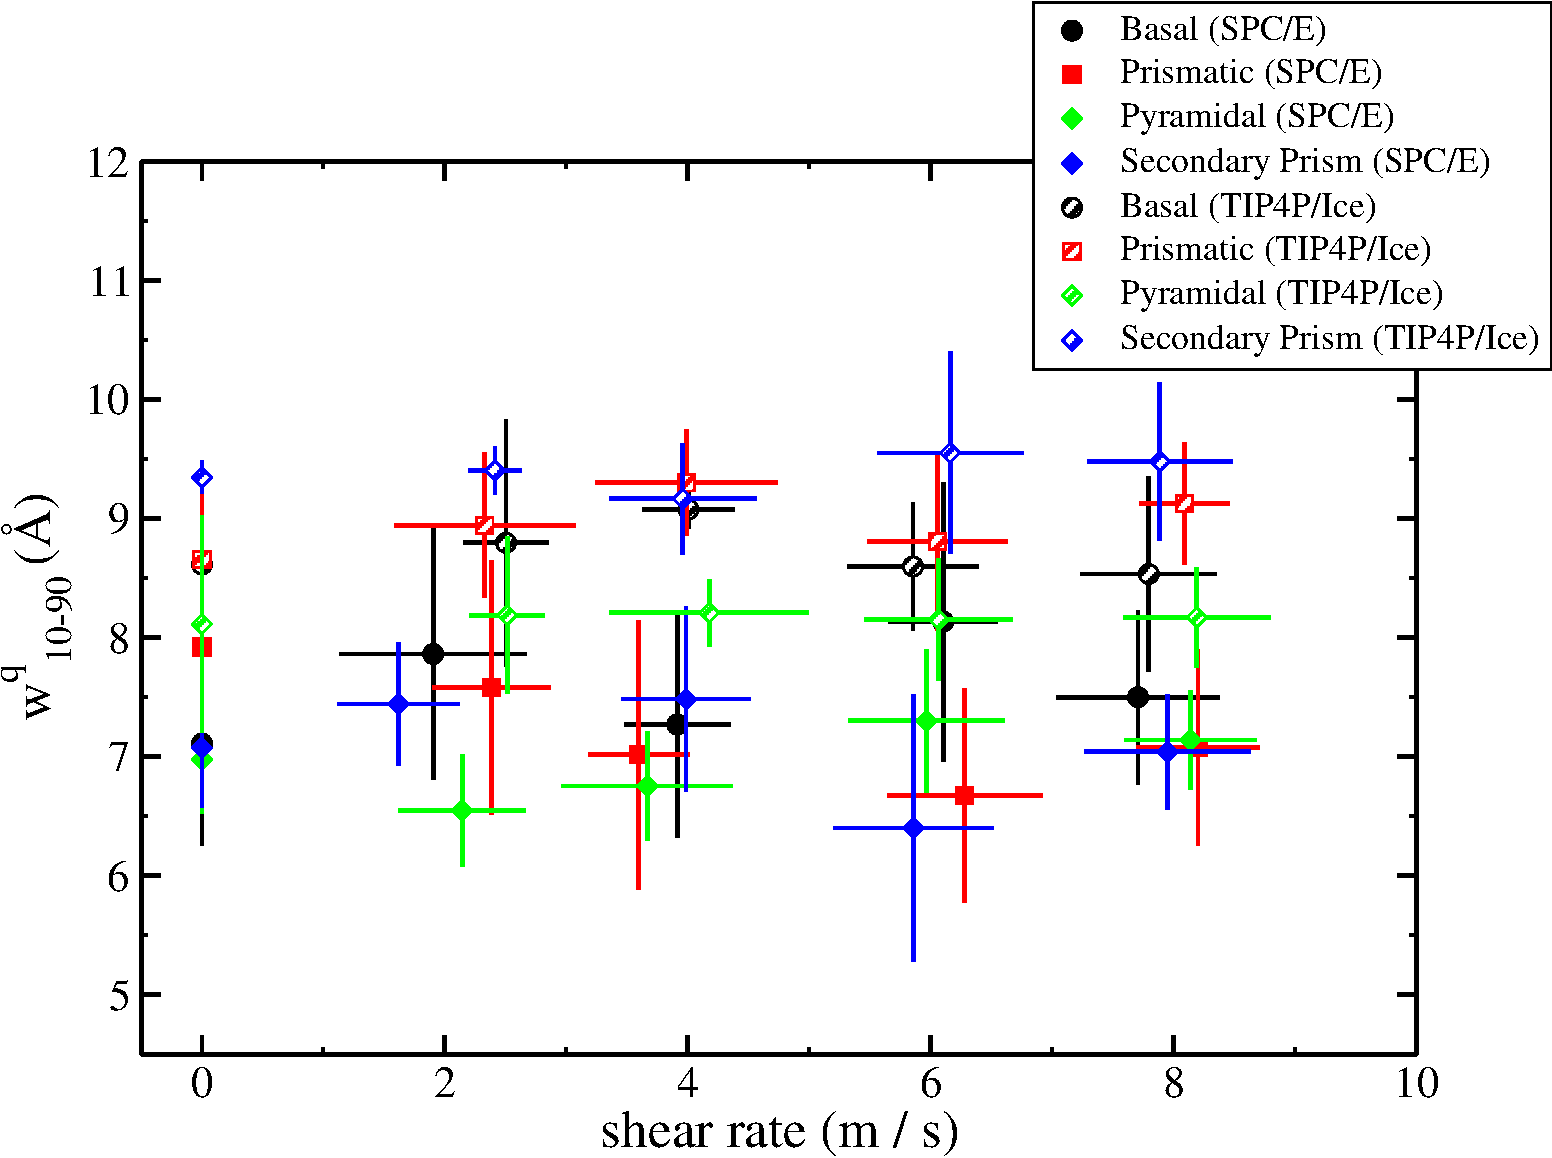
\includegraphics[width=\linewidth]{Figures/tetByShearRate}
\caption{\label{fig:tetByShearRate}The $10\%-90\%$ widths of the
  ice-I$_\mathrm{h}$ / water interface for the basal, prismatic,
  14\degree~pyramidal, and secondary prism crystal faces as determined
  by the local tetrahedral order parameter fit by
  Equation \eqref{tet_fit}.}
\end{figure*}


\section{Discussion}
While there has been a considerable number of computational and
experimental investigations on the ice / vapor
interface\cite{Bolton2000,Conde2008,Gladich2011,Sazaki2011,Pfalzgraff2011,Watkins2011,Bartels-Rausch2014,Gladich2015,Murata2015,Asakawa2016,Benet2016,Murata2016,Neshyba2016,Limmer2016,Michaelides2017,Sancheza2017},
significantly fewer studies have been reported at the ice / liquid
interface. \cite{Beaglehole1980,Karim1988,Karim1990,Hayward2001,Hayward2002,Bryk2002,Gay2002}
Due to the difficulty of experimentally probing water's properties at
the bulk liquid / solid interface, most of what is known has been
provided by computational methods. However, there is disagreement
amongst the community as to which water model is best suited for
studying these
interfaces\cite{Sanz2004a,Vega2005c,Abascal2007,Vega2009}, as well as
the coexistence temperatures for these
models.\cite{Gao2000,Bryk2004,Sanz2004a,Vega2006a,Abascal2007,Paesani2016}
Slight changes in the treatment of the long range electrostatic
interactions have been seen to significantly alter the coexistence
temperature.\cite{Bryk2004} This has resulted in a collection of data
points for the properties of water molecules at the ice / water
interface, many with different models, electrostatic treatment, and at
varying temperatures.

In the late 1980's, Karim and Haymet investigated the solid to liquid
transition for a basal ice-I$_\mathrm{h}$ / water interface using the
TIP4P model at 240~K~\cite{Karim1987,Karim1988}, and the SPC model at
200~K.\cite{Karim1990} In each of the studies, they computed the
average density along the dimension normal to the interface, and
binned the resulting profiles to coincide with the
spacing of the crystallographic planes inside their ice crystal. Karim
and Haymet then estimated the width of the basal ice-I$_\mathrm{h}$ /
water interface to be $\sim$ 10 \AA~ - 15 \AA~ by counting the number of
these large bins. This result proved to be invarient of the exposed
surface area of the basal plane.

Around the same time, Nada and Furukawa observed a slight anisotropy
between the basal and prismatic ice / water interface using the TIP4P
model at 230~K.\cite{Nada1995} Their primary method for discriminating
ice-like and liquid-like molecules was the local density, as well as
an existence function which determined the likelihood that a water
molecule had four nearest neighbors. They estimated the ice / water
interface to be between 9 \AA~ and 12 \AA~ wide, with the basal
interface being slightly narrower than the prismatic.

Our density based estimates for the basal and prismatic
ice-I$_\mathrm{h}$ / water interfaces agrees well with those by Haymet
\textit{et al.} and Nada \textit{et al.}. We did not observe the same
anisotropy as Nada and Furukawa, however, our fit resolution was much
larger, and their results could have been an artificat of their larger
binning method. 

The problem of ice / water coexistence was later revisited by Hayward
and Haymet, where a comparitive study of the basal, prism,
14\degree~pyramidal, and $\{2\bar{1}\bar{1}0\}$ secondary prism
ice-I$_\mathrm{h}$ / water interfaces was conducted.\cite{Hayward2001}
This was the first computer investigation of the 14\degree~pyramidal,
and $\{2\bar{1}\bar{1}0\}$ secondary prism ice-I$_\mathrm{h}$ / water
interfaces, providing the initial insights to the structure and
dynamics of molecules at these higher-order crystal facet
interfaces. % These two interfaces were found to be of particular
% interest as Type 1 antifreeze proteins in both winter flounder and
% shorthorn Sculpin inhibit ice growth at these ice
% surfaces.\cite{Knight2001,Wierzbicki1996,Haymet1998,Harding1999}
They observed a stable ice / water interface at 270~K over 300 ps
using the CF1 central force model, and estimated the $10\%-90\%$ width
of the interfaces by measuring the transition of two structural
criteria, the translational order and a Gaussian filtered
translational order (see Table \ref{tab:structCompare}). Their
calculations indicate that the basal and prismatic interfaces are
wider than the two higher index facets. While we did not see this
trend, our results for the basal and prismatic interfaces using the
TIP4P/Ice water model agree well with their estimates given by the
translational order parameter. Our simulations with the SPC/E model
predict a slightly thinner interface, possibly due to the colder
coexistence temperature. Lastly, their estimates of interfacial width
from the average density predicts a much wider interface, with
estimates roughly a factor of 2 larger than those computed by the
unfiltered translational order parameter. It is unclear if the
filtering process provides a more accurate measure, much of the
observed difference can be attributed to how the Gaussian filtering
process broadens out the transition between the bulk ice and bulk
liquid domains.
 

% For each order
% parameter studied, the systems were divided into $\sim$3 \AA~ bins
% along the dimension normal to the interface (chosen here to be along
% the $z$-axis), and the average of the parameter was computed for each
% bin. A Gaussian filter was then applied to the Fourier transofrm of
% the resulting order parameter profile. For example, for the
% translational order profile $\rho (z)$,
% \begin{equation}
% g(k) = \int_{-n}^{n} \mathrm{exp}(-2\pi ikz)\rho (z)dz
% \end{equation}
% where $n$ is half of the box length in the direction normal to the
% interface. The oscillations in $g(k)$ are then dampened with the
% Gaussian filter,
% \begin{equation}
% g'(k) = g(k)\mathrm{wt}(k)
% \end{equation}
% where 
% \begin{equation}
% \mathrm{wt}(k)=\frac{1}{\sigma_{k}\sqrt{2\pi }}~\mathrm{exp}\Bigg(-\frac{1}{2\sigma_{k}^{2}}k^{2}\Bigg).
% \end{equation}
% Here, $2\sigma_{k}$ defines the resolution of the Gaussian. Inverse
% Fourier transform of $g'(k)$ gives the filtered translational order
% profile, $\rho '(z)$
% \begin{equation}
% \rho '(z) = \int_{-n}^{n} \mathrm{exp}(2\pi ikz)g'(k)dk
% \end{equation}
% which can be written as a convolution integral
% \begin{equation}
% \rho '(z) = \int_{-n}^{n} \mathrm{wt}'(z-z')\rho (z')dz'
% \end{equation}
% where
% \begin{equation}
% \mathrm{wt}'(z-z') = \frac{1}{\sigma
%   \sqrt{2\pi}}~\mathrm{exp}\Bigg(-\frac{1}{2\sigma^{2}}(z-z')^{2}\Bigg)
% \end{equation}
% and the value of $\sigma$ is chosen such that $\rho '(z)$ is flat in
% the bulk ice region. This method of filtering the binned order
% parameter data ensures the profile smoothly varies from bulk ice to
% bulk liquid through the interface.  The filtered order parameter
% profiles were then averaged about the midpoint of the system, and fit
% by
% \begin{equation}
% \rho (z) = \rho_{l}[1-f(z)]+\rho_{s}f(z)
% \end{equation}
% where
% \begin{equation}
% f(z) = \frac{1}{2}\Bigg[1-\mathrm{tanh}\Big(\frac{z-z_{0}}{w}\Big)\Bigg]
% \end{equation}
% here, $\rho_{l}$ and $\rho_{s}$are the bulk densities of the liquid
% and solid, $z_0$ is the midpoint of the interface, and $w$ can be
% related to the 10-90 with of the interface through
% $w_{10-90} = 2.1971\times w$. When substitutions are made, the
% resulting expression is similar to Equation \eqref{rho_fit}.
% \begin{equation}\label{eq:Hayward2001}
% \rho (z) = \rho_{l} + \frac{\rho_{s} -
%   \rho_{l}}{2}\Bigg[1-\mathrm{tanh}\bigg(\frac{z-z_0}{w}\bigg)\Bigg]
% \end{equation}

% From Equation \eqref{eq:Hayward2001}, 
Hayward and Haymet estimated the $10\%-90\%$ widths of the
ice-I$_\mathrm{h}$ / water interface for the translational profiles
and the average density profiles (see Table
\ref{tab:structCompare}). Their calculations indicate that the basal
and prismatic interfaces are wider than that of the two higher index
facets. While we did not see this trend, our results for the basal and
prismatic interfaces using the TIP4P/Ice water model agree well with
their estimates given by the translational order parameter. Our
simulations with the SPC/E model predict a slightly thinner interface,
possibly due to the colder coexistence temperature. Lastly, their
estimates of interfacial width from the average density predicts a
much wider interface, with estimates roughly a factor of 2 larger than
those computed by the unfiltered translational order parameter. It is
unclear if the filtering process provides a more accurate measure,
much of the observed difference can be attributed to how the Gaussian
filtering process broadens out the transition between the bulk ice and
bulk liquid domains.

% In a follow up paper, Hayward and Haymet studied the orientational
% ordering of water molecules transverse to the interface as an
% additional order parameter.\cite{Hayward2002} They computed the
% time-averaged one-body orientational correlation functions for the
% angle made between the origin of the simulation cell and the HOH
% bisector, $\theta$, as well as the angle made with the projection of
% the HOH bisector with the plane of the system, $\phi$.


\begin{table}[H]
\centering
\caption{STRUCTURAL MEASURES OF THE ICE-I$_\mathrm{h}$ / WATER
  INTERFACE \label{tab:structCompare}} 
\begin{tabular}{l|cccc}
\hline  
\hline
& Basal & Prismatic & 14\degree~Pyramidal & Secondary Prism \\
\hline
Translational (CF1 270~K)\footnotemark[1] & 9.9 & 8.6  & 7.9 & 6.6 \\
Average Density (CF1 270~K)\footnotemark[1] & 18.2 & 13.6 & 11.4 & 12.3 \\
Orientational (CF1 270~K)\footnotemark[2] & 5.7 & 7.7 & 7.5 & 5.1 \\
\\
Density (TIP4P/2005 248.5~K)\footnotemark[3] & 13~-~16 & 13~-~16 & - &
                                                                    13~-~16 \\
\\
Translational (SPC/E 225~K)\footnotemark[4] & 10.54 & 8.30 & - & - \\
Density (SPC/E 225~K)\footnotemark[4] & 12.86 & 10.03 & - & -
\\
Tetrahedral (SPC/E 225~K)\footnotemark[5] & 11 & 11 & - & - \\
\\
Density (TIP4P 230~K)\footnotemark[6] & 9 & 12 & - & - \\
Translational (TIP4P 240~K)\footnotemark[7] & 5.93 & - & - & - \\
Density (TIP4P 240~K)\footnotemark[8] & 10~-~15 & - & - & - \\
\\
Translational (SPC 200~K)\footnotemark[9] & 8.13 & - & - & - \\
\\
Experimental (Ellipticity 273~K)\footnotemark[10] & 10 & 10 & - & - \\
\hline
\hline
\end{tabular}
\flushleft
Interfacial widths are reported in \AA~. \\
  \footnotemark[1]\footnotesize{Reference \cite{Hayward2001}.} \\
  \footnotemark[2]\footnotesize{Reference \cite{Hayward2002}.} \\
  \footnotemark[3]\footnotesize{Reference \cite{Benet2014}.} \\
  \footnotemark[4]\footnotesize{Reference \cite{Bryk2002}.} \\
  \footnotemark[5]\footnotesize{Reference \cite{Bryk2004}.} \\
  \footnotemark[6]\footnotesize{Reference \cite{Nada1995}.} \\
  \footnotemark[7]\footnotesize{Reference \cite{Karim1988}.} \\
  \footnotemark[8]\footnotesize{Reference \cite{Karim1987}.} \\
  \footnotemark[9]\footnotesize{Reference \cite{Karim1990}.} \\
  \footnotemark[10]\footnotesize{Reference \cite{Beaglehole1993}.} \\
\end{table}

Using the SPC/E model, Bryk and Haymet estimated interfacial widths
for the basal and prismatic faces by observing the transition of a
similar tetrahedral order parameter from the ice-like value of $0.9$
to a bulk liquid value of $0.6$.\cite{Bryk2004} This resulted in widths of
$\sim$ 11~\AA~, somewhat larger than our current estimates. While
the oxygen atoms of the presented surface facets are identical to
those used in our investigation, the surface hydrogen placement was
vastly different than ours. Our ice surfaces were designed to
replicate proton striping observed by Buch \textit{et al.} to
replicate sum-frequency generation experiments by Shultz \textit{et
  al.}.  More careful analysis will be necessary to determine if the
proton striped surface configurations used here are the origin of this
discrepancy.


\section{Summary}
In this chapter we have presented structural analyses of the basal,
prismatic, 14\degree~ pyramidal, and secondary prism facets of an
ice-I$_\mathrm{h}$ / water interface. Fitting the local density
profiles predicted a $10\%-90\%$ interfacial width of $\sim$ 8 \AA~
for the basal and two prismatic facets. However, the same fits
predicted a much narrower interface for the pyramidal facet, believed
to be due to the rotation of the crystal. Fitting these density
profiles required biasing the density maxima within the ice, therefore
a second order parameter was considered. The local tetrahedral order
parameter is a more accurate measure of liquid-like and ice-like
configurations, and fits of the order parameter gave estimates of
interfacial width with smaller error. For each of the facets, the
SPC/E ice-I$_\mathrm{h}$ / water interface was found to be $\sim$ 7
\AA~ wide, while the slightly warmer TIP4P/Ice interface was predicted
to be $\sim$ 9 \AA~ wide. These widths were found to be insensitive to
shear rate, indicating that the interface is quite stable under flow.


%%%%%%%%%%%%%%%%%%%%%%%%%%%%%%%%%%%%%%%%%%%%%%%%%%%%%%%%%%%%%%%%%%%%%%%%%%%%%%%%%%%
%		CHAPTER 4 -- Dynamic Widths of Ice / Water Interfaces
%%%%%%%%%%%%%%%%%%%%%%%%%%%%%%%%%%%%%%%%%%%%%%%%%%%%%%%%%%%%%%%%%%%%%%%%%%%%%%%%%%%
\chapter{DYNAMIC WIDTHS OF ICE-I$_\mathrm{h}$ / WATER INTERFACES}\label{chap:Dyn}
In Chapter \ref{chap:Str}, estimates of the ice-I$_\mathrm{h}$ / water
interface were obtained by determining the distance over which
structural order parameters transitioned from their bulk liquid values
to those for ice-like configurations. The density and local
tetrahedral order parameter were found to transition smoothly between
the two regions, and yield similar widths for a given facet.
Simulations and experiments indicate that the dynamics of water
molecules depend not only on their local structure and environment,
but also on the ordering of molecules outside of their first solvation
shell. Given this, we have investigated the transition of the dynamics
of water molecules across the interface as well.


\section{Dynamic Measures of an Ice / Water Interface Under Shear}\label{structure}

\subsection{Diffusion Coefficients as a Measure of Interfacial Width}
Compute diffusion coefficients as a function of distance through
interface. Plot, fit, etc.

\subsection{Reorientation of Water Molecules}
The spatially-resolved orientational time correlation function,
\begin{equation}\label{C(t)1}
  C_{2}(z,t)=\langle P_{2}(\mathbf{u}_i(0)\cdot \mathbf{u}_i(t))
  \delta(z_i(0) - z) \rangle,
\end{equation}
provides local information about the decorrelation of molecular
orientations in time. Here, $P_{2}$ is the second-order Legendre
polynomial, and $\mathbf{u}_i$ is the molecular unit vector that bisects
the HOH angle of molecule $i$. The angle brackets indicate an average
over all the water molecules and time origins, and the delta function
restricts the average to specific regions in the $z$-dimension. 

In the ice crystal, decay of $C_2(z,t)$ is incomplete, while in the
liquid, correlation times are typically measured in ps. Observing the
spatial transition between the decay regimes can define a dynamic
measure of the interfacial width. To determine dynamic widths of the
interfaces under shear, each of the systems were divided into bins
along the $z$ axis ($\approx$ 1 \AA\ wide) and $C_2(z,t)$ was computed
using only those molecules that were in the bin at the initial
time. For each ice / water interface investigated, the following 0.5
ns simulations were computed: quiescent simulations (where no thermal
or momentum gradient was present), simulations with only a thermal
gradient present, and simulations where both thermal and momentum
gradients were present. During these simulations, the positions and
orientations of each molecule were recorded every 100 fs.

\begin{figure}
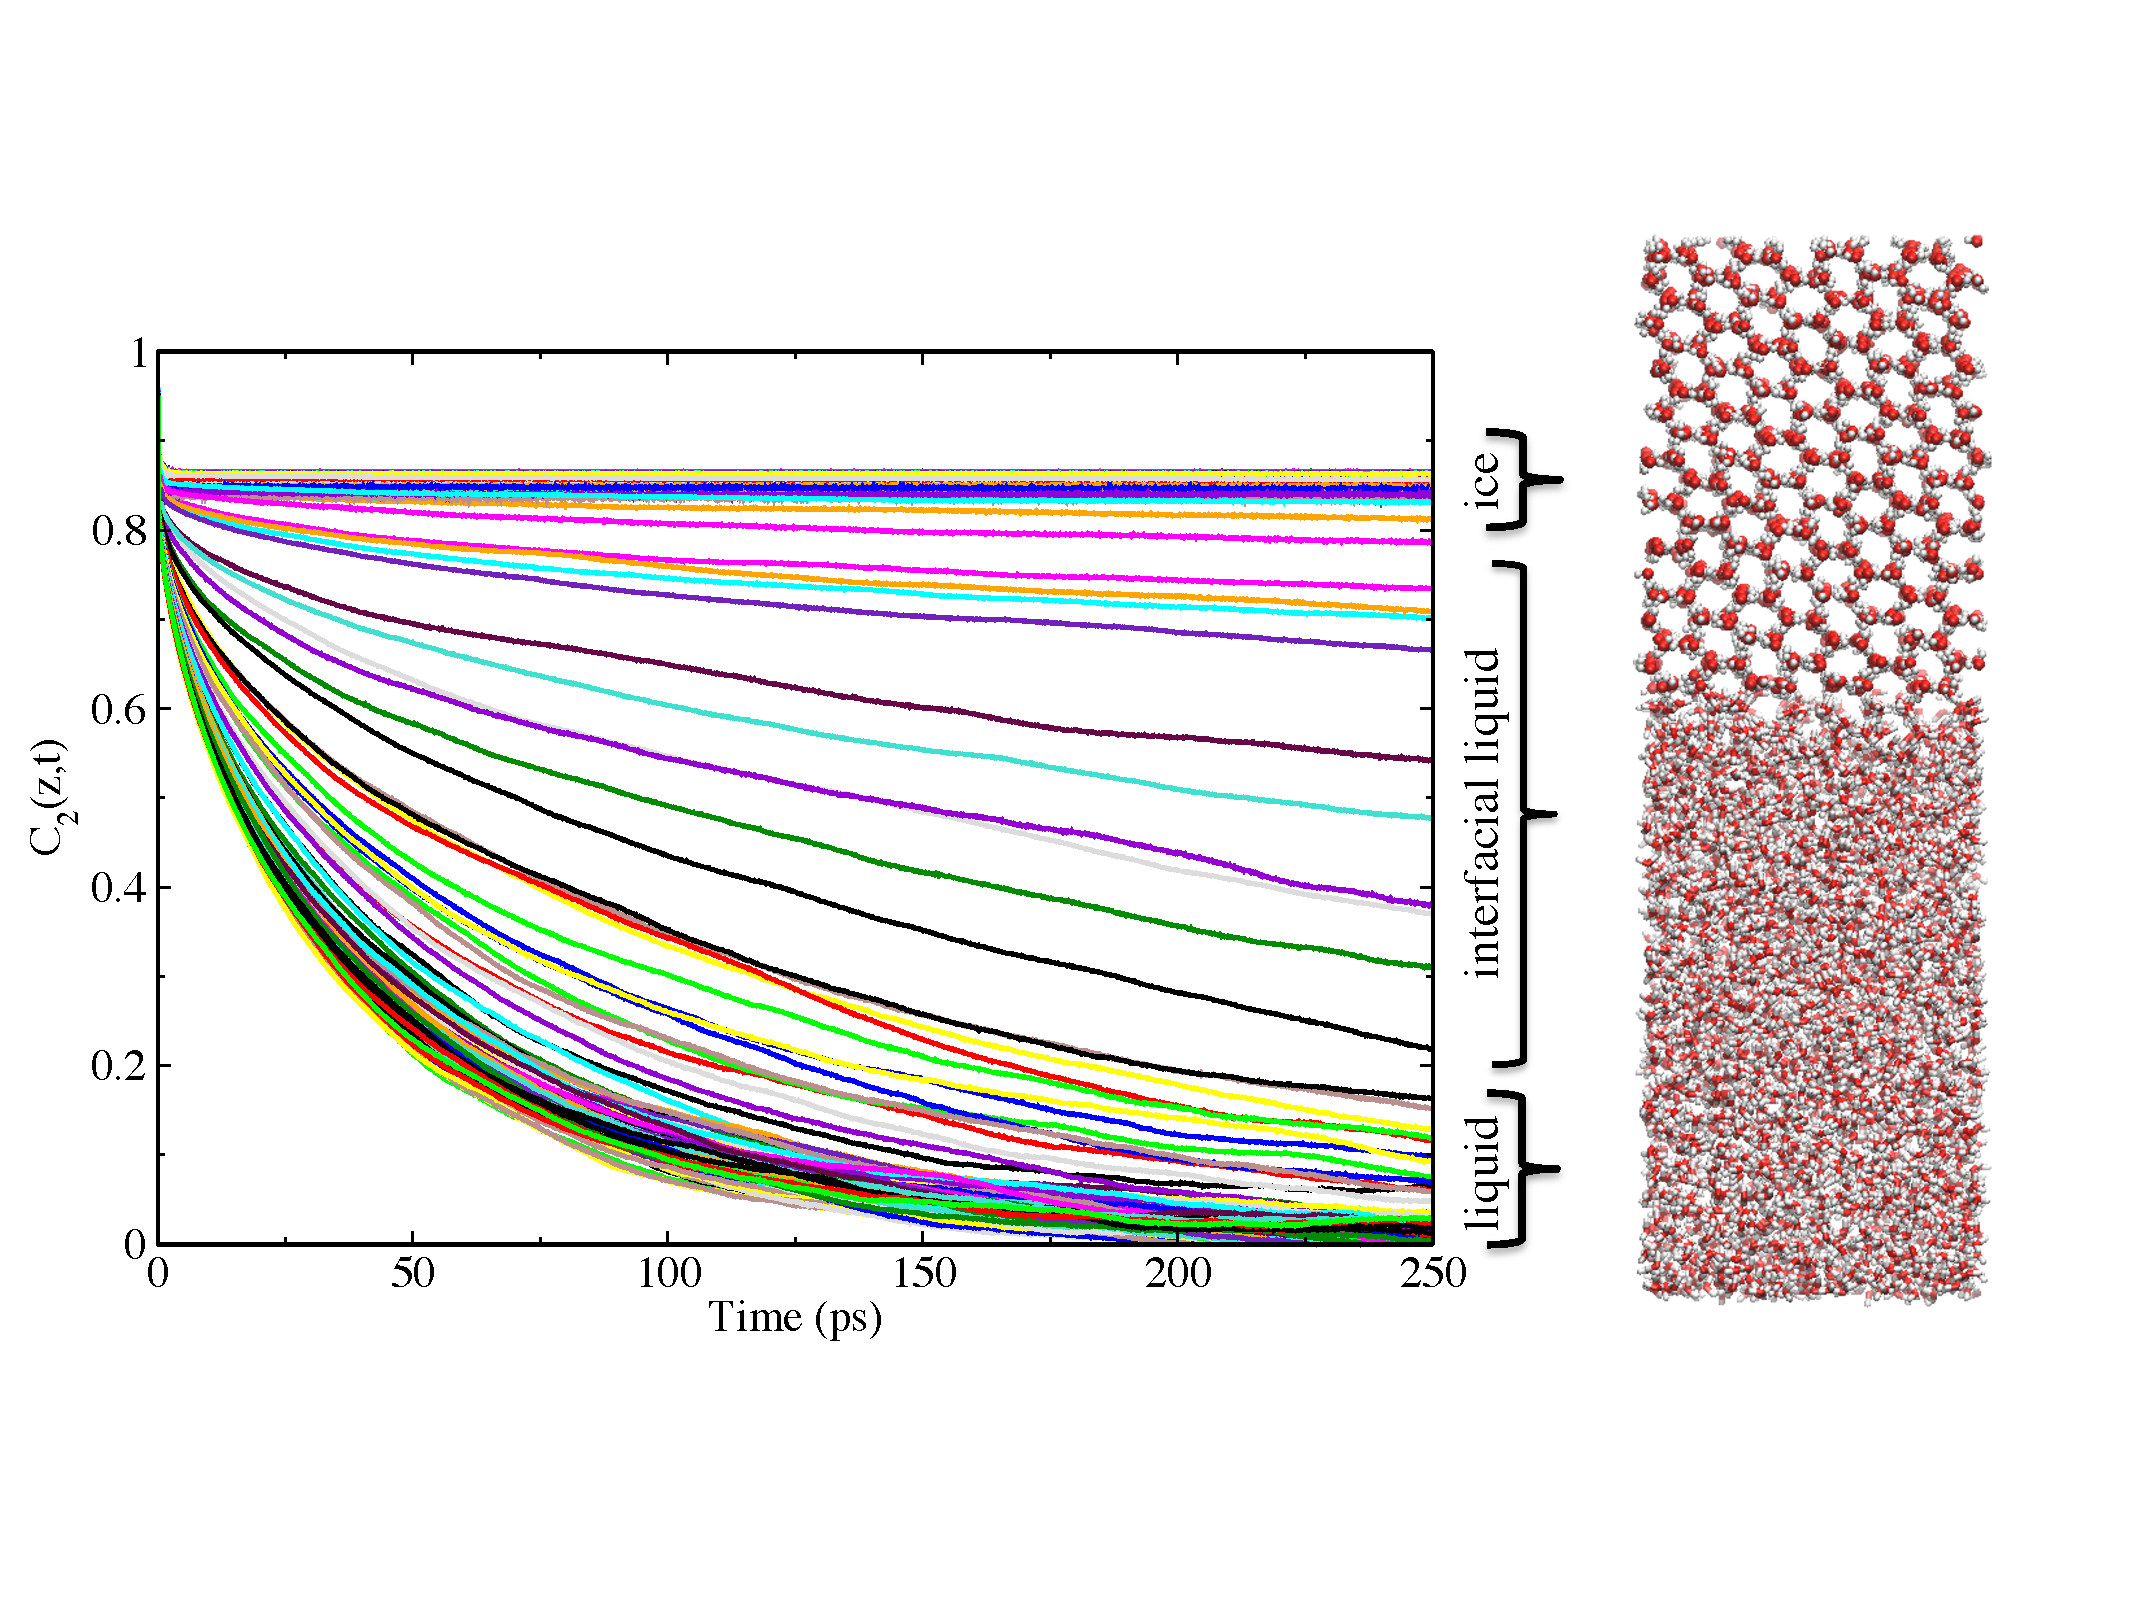
\includegraphics[width=\linewidth]{Figures/CztImage}
\caption{\label{fig:Czt} $C_2(z,t)$ collected in 1 \AA~bins across the SPC/E
  secondary prism ice / water interface. The band that experiences very
  little decay represents water molecules in the ice, while the band
  that decays quickly corresponds to bins in the liquid.  The
  correlation function presents a continuous distribution of decay
  behaviors across the interface between ice and liquid water.}
\end{figure}

Recently, Laage and Hynes have determined the mechanism for water
reorientation.\cite{Laage2006,Laage2008} Using molecular dynamics
simulations, they found that water reorients by breaking a hydrogen
bond with an overcoordinated first-shell neighbor, and makes a large
angle jump to form a new hydrogen bond with an undercoordinated
second-shell neighbor. The hydrogen bond cleavage and molecular
reorientation occur in a concerted fashion, not in successive steps as
was previously thought. With this detailed picture, they constructed
the Extended Jump Model\cite{Laage2006,Laage2008} based on the Ivanov
Jump Model and parameters extracted from their molecular simulations;
the average jump amplitude of the rotational jump, $\theta_{0}$, and
the frequency of the jumps, $1/\tau_{0}$. After accounting for
molecular frame reorientation, the Extended Jump Model is able to
predict reorientation relaxation times, $\tau_{n}^{jump}$, which agree
with experimental results as well as estimates obtained from
simulations where fast librational motion is ignored.

Computed $C_2(z,t)$ values have previously been fit to a
triexponential decay, with three time constants:
$\tau_\mathrm{short}$, measuring the librational motion of the water
molecules, $\tau_\mathrm{middle}$, measuring the timescale for the
large angle jumps during the breaking and making of hydrogen bonds,
and $\tau_\mathrm{long}$, corresponding to the translational motion of
the water molecules.\cite{Louden2013a} The Extended Jump Model also
includes three similar decay constants, however two of them are linked
and the dynamics of the decay is governed by two parameters. Since we
are interested in how the decay times and the individual contributions
may change through the interface, we have fit the $C_2(z,t)$ data
with
\begin{equation}
  C_{2}(z,t) = a~e^{-t/\tau_\mathrm{short}} + b~e^{-t/\tau_\mathrm{middle}} + 
  (1-a-b)~e^{-t/\tau_\mathrm{long}}
\label{eq:c2}
\end{equation}
where all of the decay constants are considered local functions of the
$z$ coordinate. In Fig. \ref{fig:SPorient}, the $z$-coordinate
profiles for the three decay constants, $\tau_{\mathrm{short}}$,
$\tau_{\mathrm{middle}}$, and $\tau_{\mathrm{long}}$ for the secondary prism interface
is shown, along with their fractional components of the overall total
decay, ($a$, $b$, $1-a-b$), respectively. Similar figures for the
other interfaces are provided in the Supporting Information.

In the liquid regions of all four interfaces, $\tau_\mathrm{middle}$
and $\tau_\mathrm{long}$ consistently approach $3-6$ ps and $30-40$
ps, respectively.  Both of these times increase closer to the
interface.  Conversely, $\tau_\mathrm{short}$ decreases from a
liquid-state value of $72-76$ fs approaching the interface.

The fractional contributions of the three motions to the overall decay
changes as we approach the interface as well. Far from the ice, the
librational motion and hydrogen bond breaking/making events each
contribute to about 20 percent of the total decay, whereas frame
reorientation contributes about 60 percent. As we approach the
interface, the librations and hydrogen bond dynamics both decrease in
contribution. The librations comprise approximately 15 percent of the
overall decay at the edge of the interface, whereas the hydrogen bond
contributions drop to approximately zero. In contrast, the fraction of
the total decay due to frame reorientation is shown to increase
approaching the interface.  The time constant corresponding to this
motion is seen to logarithmically increase as we approach the interface
as the molecules become more ice-like. In the ice we would expect
molecular reorientation to be incomplete, however, at the interface we
observe frame reorientation to contribute 85 percent of the overall
decay.


\begin{figure}
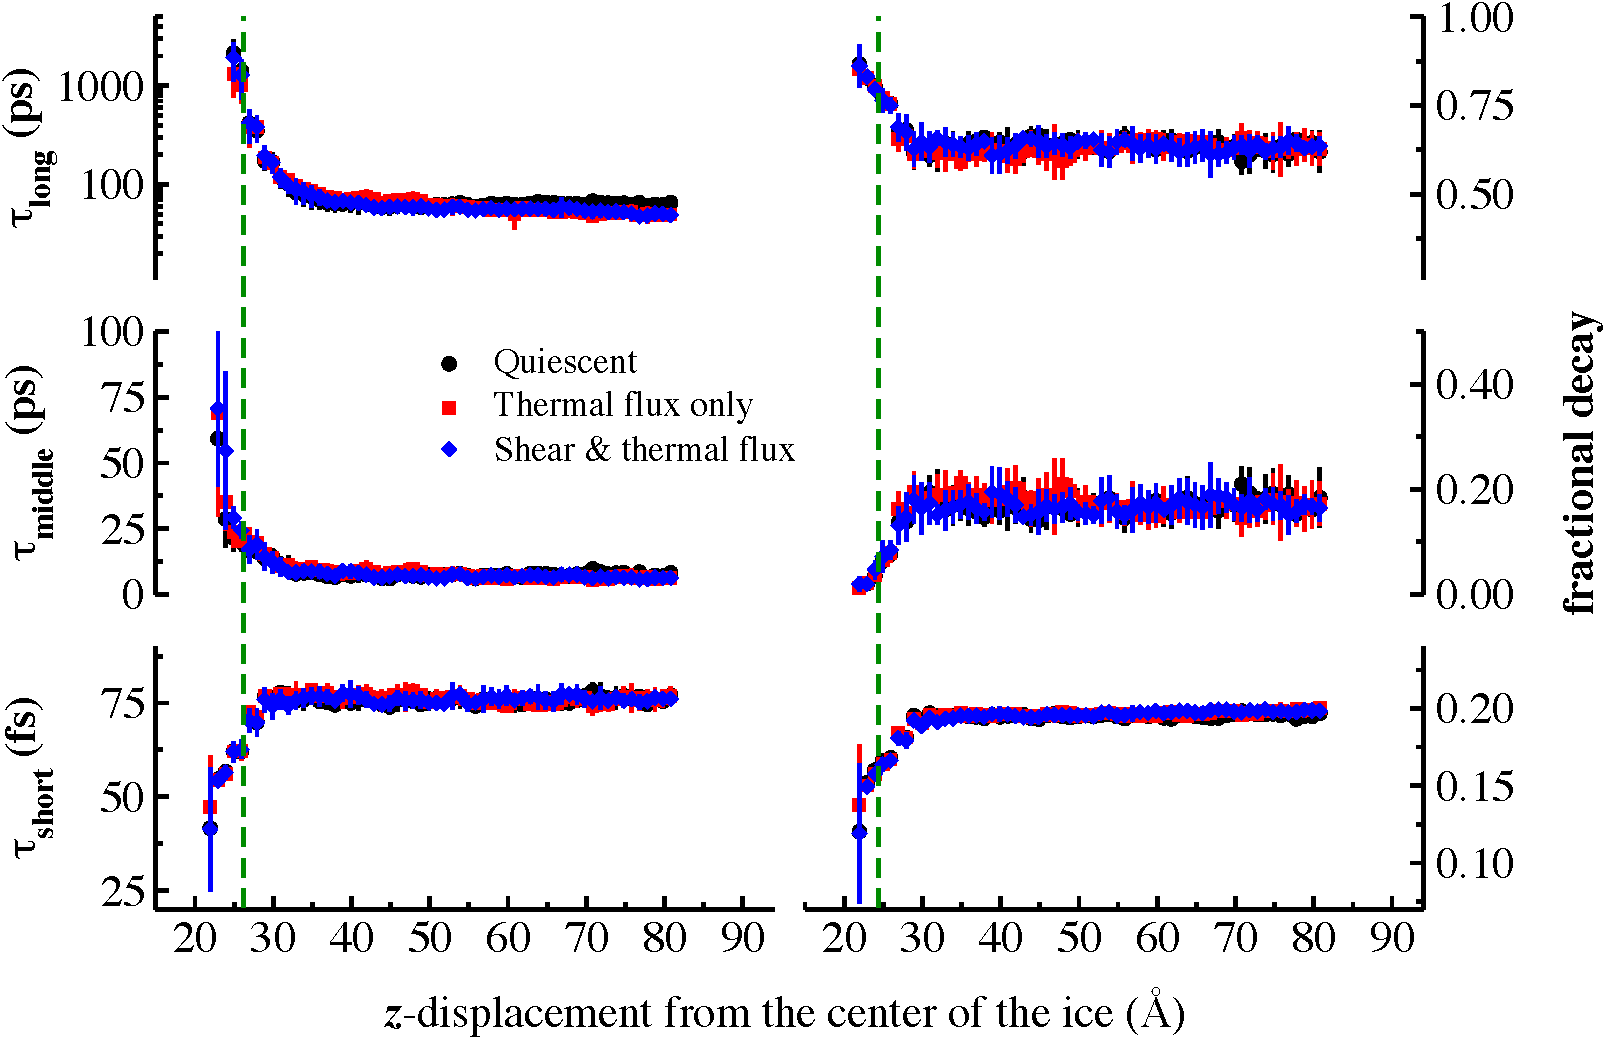
\includegraphics[width=\linewidth]{Figures/Sec_lcorrz}
\caption{\label{fig:SPorient} Decay times (left) for $C_2(z,t)$ at the
  SPC/E secondary prism interface, and their fractional contributions to the
  overall decay (right) fit using Eq. \eqref{eq:c2}. The local decay
  constants are plotted as a function of distance from the center of
  the ice slab. The vertical dashed line indicates the Gibbs dividing
  surface determined using the local tetrahedral order parameter.
  Results are shown for a quiescent system with no applied kinetic or
  momentum flux (black), an interface with an imposed
  kinetic energy flux (red), and a sheared simulation (blue) with both
  kinetic and momentum fluxes.}
\end{figure}

The middle and long decay times diverge inside the ice crystal, so the
orientational rate, $k(z) = 1 / \tau(z)$ can be used to identify a
dynamic interfacial width for the interface by fitting the profiles of
the middle and long-time orientational rates with a function that goes
smoothly between bulk-like liquid behavior and the crystal,
\begin{equation}\label{tauFit}
  k(z) = \frac{1}{\tau_\mathrm{liquid}} - \frac{1}{2~\tau_\mathrm{liquid}} \left(
      \tanh \left( \frac{z-l}{d} \right) - \tanh \left( \frac{z-r}{d} \right) \right)
\end{equation}
where $l$ and $r$ are the locations of the Gibbs dividing surfaces,
and $d$ is a dynamic width.  As with the structural widths,
$10\%-90\%$ dynamic widths are easily computed from the fits
($d_\mathrm{10-90} = 2.197~d$).  These values are provided in Tables
\ref{tab:propsSPCE} and \ref{tab:propsTIP4P}. All four SPC/E
interfaces exhibit dynamic widths that are $\sim 11$~\AA, and are
larger than the structural widths computed above.  In TIP4P/Ice at
270K, the dynamic widths are $\sim 14$~\AA, also larger than the
structural widths in for these interafaces.

We note that Bryk and Haymet also calculated the orientational time
correlation function at the basal interface of SPC/E
water,\cite{Bryk2002} and observed the same qualitative trend through
the ice / water interface, although the spatial resolution was not
sufficient to resolve a dynamic width.
 
\subsection{Spatial resolution of Hydrogen bond jump rates}
The spatially-resolved hydrogen bond jump correlation function,
\begin{equation}\label{jump}
C_\mathrm{jump}(z,t) = 1 - \langle n_a(0) n_b(t) \delta(z_i(0) - z) \rangle
\end{equation}
measures the decorrelation of a hydrogen bond on molecule $i$ as it
transitions between one acceptor ($a$) and another ($b$). $n_a(0)$ is
set to one if hydrogen $i$ is bound to acceptor $a$ at time $0$, and
is zero otherwise.  Absorbing boundaries are utilized with this
correlation function; switches from $b$ back to $a$ at a later time
are considered a new jump, and the angle brackets indicate an average
over all donor hydrogens and time origins. Laage and Hynes determined
the bulk version of this function had \textit{single}-exponential
decay in room temperature water.

A version of this correlation function was used to investigate how
water molecules reorient around
ions\cite{Laage2007,Laage2008a,Stirnemann2011a,Laage2011},
proteins\cite{Duboue-Dijon2014}, and in confined
spaces\cite{Laage2012b,Fogarty2014}.  Laage and Hynes studied how the
strength of the hydrogen bond might perturb the reorientation
dynamics,\cite{Laage2006a} and found the librational motion which
forms a cone around the O-O vector is smaller for more strongly
hydrogen bonded water. This may also provide a partial explanation for
the increasing contribution of short time orientational decay very
close to the ice surfaces.  Since the solid creates an excluded volume
for the water molecules that are in proximity to the interface, the
hindered range of motion (i.e., a smaller cone around the O-O vector)
manifests as faster librational decay.

As an additional measure of a dynamic width of the quiescent
interfaces, each of the systems were divided into bins along the $z$
axis ($\approx$ 1 \AA\ wide) and $C_\mathrm{jump}(z,t)$ was computed
(see Fig. \ref{fig:SPkjmp} and Fig. \ref{fig:SPTIP4Pkjmp}).
Like Laage and Hynes, we find that within each spatial region, the
decay is easily fit with a single exponential, yielding a local
hydrogen bond jump time. The jump times diverge inside the ice
crystal, so the jump rate, $k_\mathrm{jump}(z) = 1 / \tau_0(z)$ can be
used to identify a hydrogen bond jump width for the interface in a
similar manner to the dynamic width. $k_\mathrm{jump}(z)$ was fit with
a hyperbolic tangent (see Eq. \eqref{tauFit}) and the 10-90 jump
width, $j_\mathrm{10-90}$, is shown in tables \ref{tab:propsSPCE} and
\ref{tab:propsTIP4P}.

\begin{figure}
\includegraphics[width=5.5in]{Figures/secPrismJumpPlot}
\caption{\label{fig:SPkjmp} Upper: Hydrogen bond jump correlation
  functions, $C_\mathrm{jump}(z,t)$, collected in 1 \AA~bins across
  the SPC/E secondary prism ice / water interface. The band that
  experiences very little decay represents water molecules in the ice,
  while the band that decays quickly corresponds to bins in the
  liquid.  The correlation function presents a continuous distribution
  of decay behaviors across the interface between ice and liquid
  water.  Lower: $C_\mathrm{jump}(z,t)$ decays exponentially, and each
  1 \AA~spatial bin can be fit with a jump rate, $k_\mathrm{jump}(z)$.
  These are shown with a fit that provides a ``jump'' width,
  $j_\mathrm{10-90}$. The locations of the structural Gibbs dividing
  surfaces (using tetrahedrality) are indicated with vertical dashed
  blue lines, while the locations of the ``jump'' interfaces are shown in
  orange.}
\end{figure}


\begin{figure}
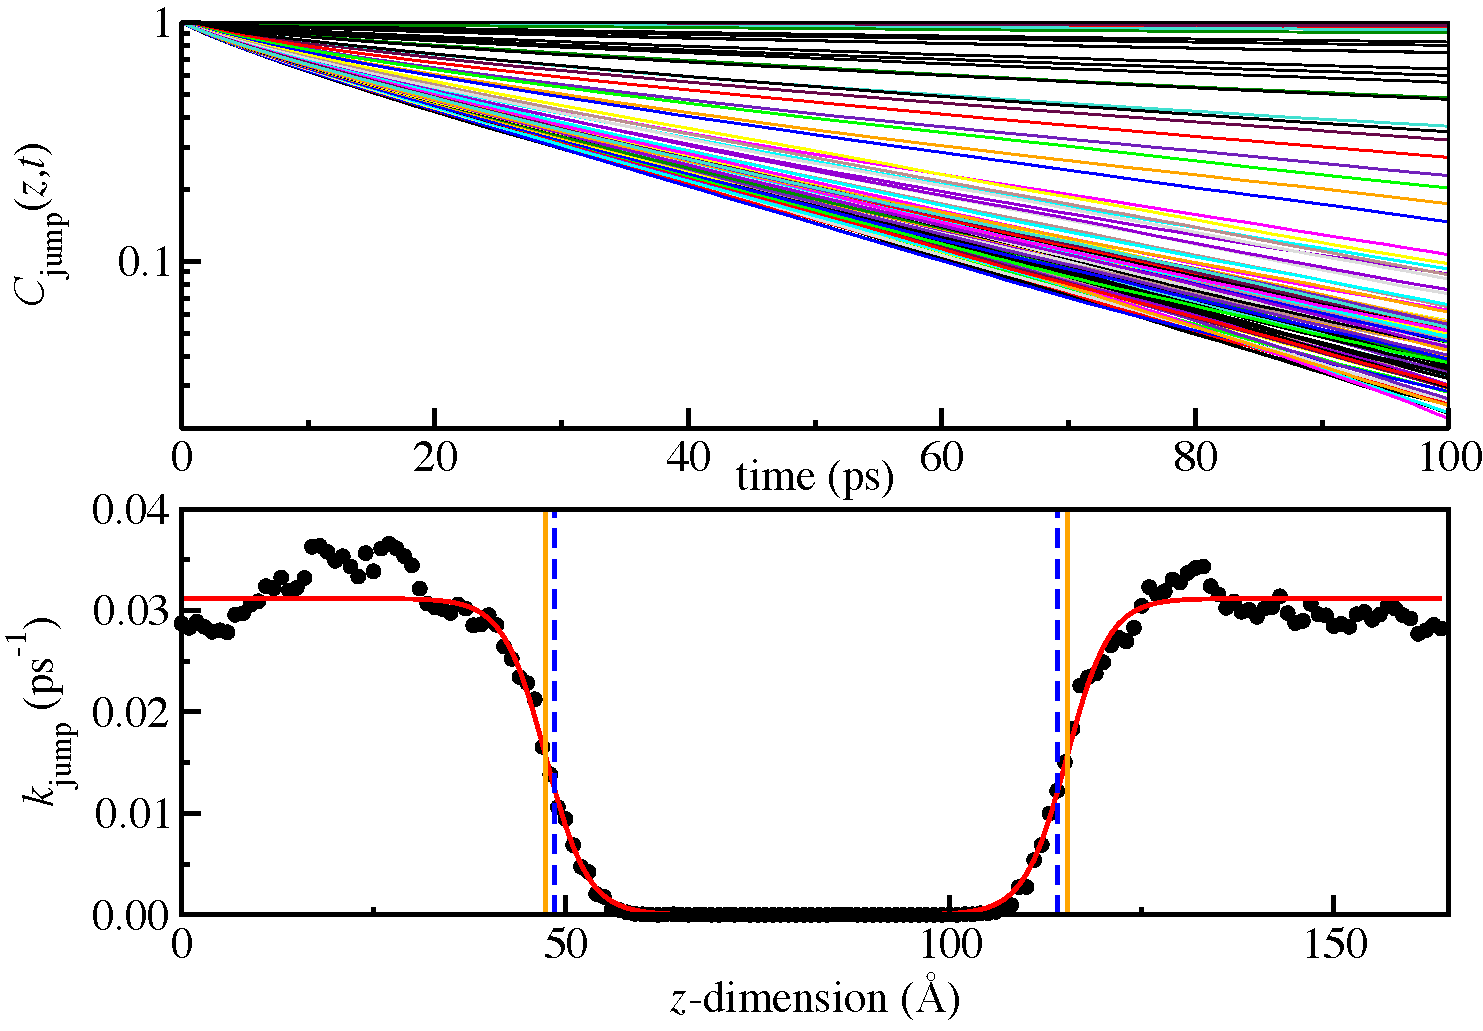
\includegraphics[width=\linewidth]{Figures/secprismJumpPlotTIP4PIce}
\caption{\label{fig:SPTIP4Pkjmp} The same secondary prism hydrogen
  bond jump data as Fig. \ref{fig:SPkjmp}, but collected using the
  TIP4P/Ice model and at 270~K.  Note that the higher coexistence
  temperature for this model increases the observed liquid-state jump
  rates, and has brought the structural and jump interfaces much
  closer together.}
\end{figure}




%%%%%%%%%%%%%%%%%%%%%%%%%%%%%%%%%%%%%%%%%%%%%%%%%%%%%%%%%%%%%%%%%%%%%%%%%%%%%%%%%%%
%		CHAPTER 5 -- Friction at Ice / Water Interfaces
%%%%%%%%%%%%%%%%%%%%%%%%%%%%%%%%%%%%%%%%%%%%%%%%%%%%%%%%%%%%%%%%%%%%%%%%%%%%%%%%%%%
% \documentclass[journal = jpccck, manuscript = article]{achemso}
% \setkeys{acs}{usetitle = true}
% \usepackage{fixltx2e}
% \usepackage{float}
% \usepackage{achemso}
% \usepackage{natbib}
% \usepackage{multirow}
% \usepackage{wrapfig}
% \usepackage{times}
% \usepackage{tablefootnote}
% \usepackage{booktabs}
% \usepackage[version=3]{mhchem}  % this is a great package for formatting chemical reactions
% \usepackage{url}
% \usepackage{graphicx}  % needed for figures
% \usepackage{dcolumn}   % needed for some tables
% \usepackage{bm}        % for math
% \usepackage{amssymb}   % for math
% \usepackage{booktabs}
% \usepackage{tablefootnote}
% \usepackage{mathptmx}

% \newcommand*{\citen}[1]{%
%   \begingroup
%     \romannumeral-`\x % remove space at the beginning of \setcitestyle
%     \setcitestyle{numbers}%
%     \cite{#1}%
%   \endgroup   
% }

\chapter[Friction at ice-I$_\mathrm{h}$ / water interfaces]{Friction at ice-I$_\mathrm{h}$ / water interfaces is governed
  by solid-liquid hydrogen-bonding} 
% \author{Patrick B. Louden}
% \author{J. Daniel Gezelter} \email{gezelter@nd.edu}
% \affiliation{Department of Chemistry and Biochemistry, University of
%   Notre Dame, Notre Dame, IN 46556} 

% \keywords{ice; water; interfaces; friction; hydrogen bonding}

% \begin{document}

% \begin{tocentry}
% \center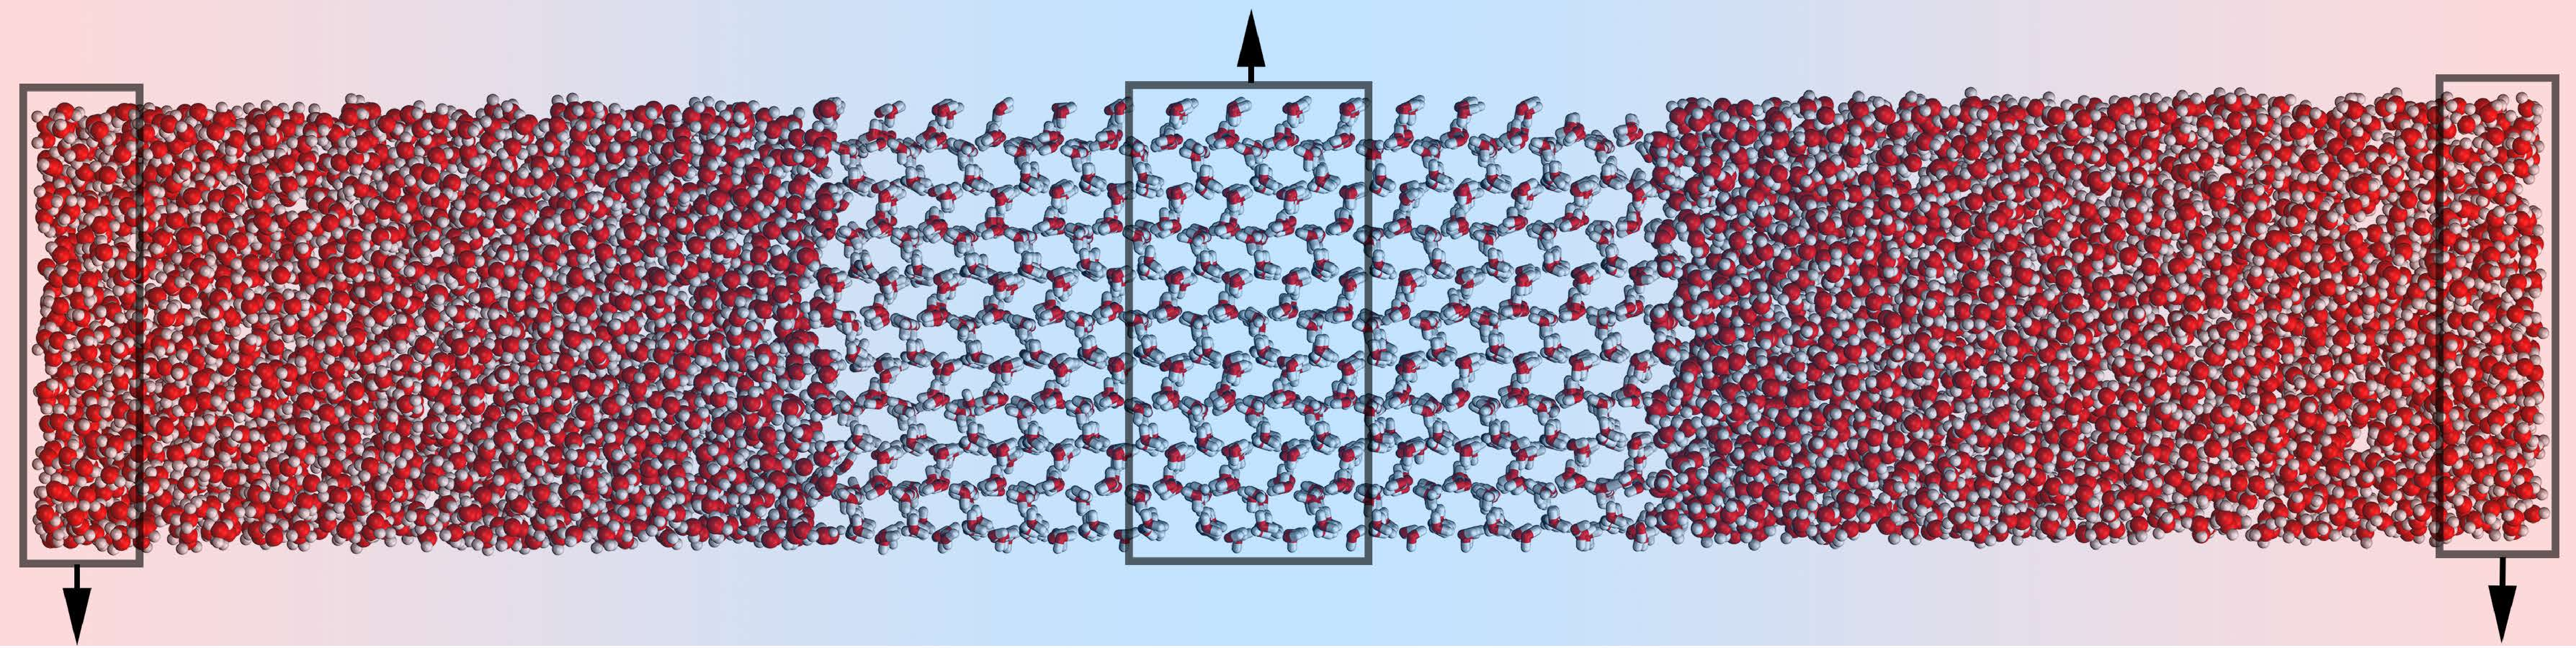
\includegraphics[width=3.25in]{ShearingTOC.pdf} 
% Simulations of ice/water interfaces suggest that interfacial friction is
% governed by the surface density of solid-liquid hydrogen bonds.
% \end{tocentry}

% \begin{abstract}
  We present evidence that the surface density of solid to liquid
  hydrogen bonds directly correlates with the solid/liquid friction of
  ice/water interfaces. Using non-equilibrium molecular dynamics
  simulations, the basal $\{0001\}$, prismatic $\{10\bar{1}0\}$,
  pyramidal $\{20\bar{2}1\}$, and secondary prism $\{11\bar{2}0\}$
  facets of ice-I$_\mathrm{h}$ were drawn through liquid water with a
  momentum flux between the solid and liquid phases. Solid to liquid
  hydrogen bonds were identified using local tetrahedral ordering of
  the water molecules. An expression for friction coefficients
  appropriate for negative slip boundary conditions is presented, and
  the computed friction of these interfaces is found to be invariant
  to the shear rate and direction of shear relative to the surface
  features. Structural and dynamic interfacial widths for all four
  facets were found to be similar, and are also independent of the
  shear rate and direction. Differences in the solid to liquid
  hydrogen bond density are explained in terms of surface features of
  the four facets.
%\end{abstract}


\section{Introduction}

Ice friction has been investigated extensively with a range
of experiments to elucidate the role of
temperature,\cite{Bowden1939,Evans1976,Roberts1981,Derjaguin1988,Liang2003,Higgins2008} sliding speed,\cite{Evans1976,Derjaguin1988,Liang2003} applied
load,\cite{Bowden1939,Oksanen1982,Derjaguin1988,Buhl2001,Baurle2006}
contact area,\cite{Bowden1939,Baurle2007} and
moisture.\cite{Calabrese1980} Kietzig \textit{et al.} performed
experiments on steel alloy rings sliding over a prepared ice
surface.\cite{Kietzig2009} They investigated the effect of surface
nanopatterning, hydrophobicity, and surface structure of the
ice-exposed slider on the ice/slider friction.
Using laser irradiation, the slider surface hydrophobicity was tuned
without changing the chemical nature of the material. Kietzig showed
that laser-induced hydrophobicity resulted in fewer capillary bridges
forming between the slider and a thin film of melted ice. This reduced
the amount of viscous shearing of the ice-melt, resulting in a lower
friction coefficient.
While ice friction experiments have focused on heterogeneous
materials,\cite{Bowden1939,Evans1976,Derjaguin1988,Liang2003,Liang2005,Baurle2006,Baurle2007,Kietzig2009,Kietzig2010}
there have also been significant advances made on understanding
ice-ice
friction.\cite{Oksanen1982,Kennedy2000,Maeno2004,Fortt2007,Fortt2011,Lishman2011,Samadashvili2013}

Experiments and computer simulations both suggest the existence of a
quasi-liquid layer (QLL) that forms at the surface of ice at
temperatures below the bulk melting point but above
235K.\cite{Kroes1992,Ikeda-Fukazawa2004,Picaud2006,Conde2008,Bartels-Rausch2014,Sancheza2017}
The formation of this layer is driven by the termination of the
periodic crystal structure. The surface molecules are not as tightly
bound to their lattice positions as molecules in the underlying ice,
and with sufficient thermal energy, these molecules reorient to
maximize hydrogen bonding. At warmer temperatures, they can also
translate along the surface.\cite{Pfalzgraff2011,Bartels-Rausch2014}
The existence of the QLL is now generally accepted as one of the
reasons that ice displays a low coefficient of sliding
friction.\cite{Dash1995,Rosenberg2005,Dash2006,Malenkov2009}

Generally, three distinct ice friction regimes have been found:
boundary friction, mixed friction, and hydrodynamic friction, and the
particular regime depends on the temperature and sliding velocity of
the
material.\cite{Bhushan2002,Kietzig2009,Kietzig2010,Persson2015,Tuononen2016}
The observed friction is the result of different physical processes in
each regime. In boundary friction, the lubricating layer of ice melt
is only a few molecules thick. This thin film is unable to support the
sliding load, and friction can be attributed to surface asperities of
the sliding material interacting with the ice surface
itself.\cite{Bhushan2002} In the mixed friction regime, the
lubricating layer is thicker than in the boundary regime, but not yet
sufficiently thick to maintain the sliding load. The QLL film reduces
solid-solid adhesion at the interface, although the lubricating layer
can also form capillary bridges with the material, resulting in a drag
force.\cite{Kietzig2009,Kietzig2010}

If the liquid layer is thick enough to support the sliding load, the
slider's surface asperities are no longer in contact with the surface
and the observed friction may be due to the capillary bridges formed
between the ice melt and the material. Under these conditions, the ice
friction is classified as hydrodynamic
friction.\cite{Kietzig2009,Kietzig2010} Thus the three regimes are
characterized by the extent that a liquid-like layer of water
mitigates the sliding load.

\begin{figure}
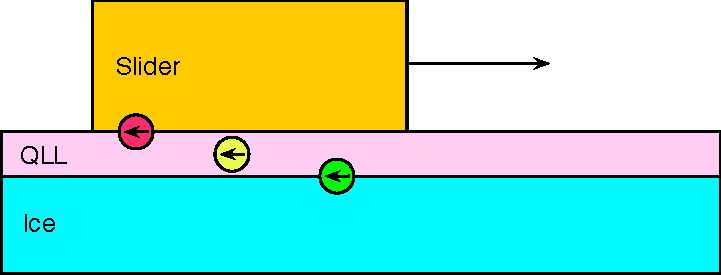
\includegraphics[width=4in]{Figures/QLLsketch}
\caption{\label{fig:QLLsketch} In the hydrodynamic regime, the
  friction felt by a slider on an ice surface is mediated by a
  quasi-liquid layer (QLL) that forms on the surface of the ice.
  There can be many contributions to this friction: capillary bridges
  between the material and the QLL (red), viscous drag in the liquid
  (yellow), and solid-liquid friction between the ice and the liquid
  film (green). This study concerns the last of the three
  contributions, the drag contributed by the ice-liquid interface.}
\end{figure}

Kietzig \textit{et al.} have outlined popular experimental techniques
used to investigate the coefficients of friction for a variety of
materials sliding on ice, as well as their sensitivity to temperature,
slider load, contact area, wettability and hydrophobicity of the
slider.\cite{Kietzig2010} Of particular interest, the friction
coefficients were found to increase with increasing slider
velocity. This was attributed to three physical processes; adhesion
forces between the slider's asperities and the ice surface, breaking
of capillary bridges between the slider and the ice surface, and the
viscous shearing of the ice melt across the ice surface. While teasing
apart the individual contributions has proven challenging,
Kietzig\cite{Kietzig2009} and Persson\cite{Persson2015,Tuononen2016}
have made significant progress. However, there is still very little
known about water shearing over ice surfaces. Open questions include:
how does the structure of the interface change during this process,
and what role does the presented crystal facet have in the observed
friction?

To help understand slider-ice friction in the hydrodynamic regime, we
have simulated the drag forces contributed by the interaction of the
liquid water film with the underlying ice facet. This study uses
non-equilibrium molecular dynamics (with an applied momentum flux) to
create a shear flow at the ice/water interface. The magnitude of the
momentum flux is then used to compute the solid-liquid friction for
four different facets of ice that are presented to the liquid.  We
have previously used this technique to study solid-liquid friction for
the basal and prismatic crystal facets where we observed significant
facet-dependence, and noted surface corrugations that could contribute
to these differences.\cite{Louden2013} Here, we broaden the
investigation to four common ice facets, we study significantly larger
systems for significantly longer times, a wider range of shear rates,
and we introduce a novel method for calculating solid-liquid friction
coefficients under conditions of \textit{negative} slip.

\section{Methodology}
\subsection{Construction of Ice / Water interfaces}
Ice I$_\mathrm{h}$ crystallizes in the hexagonal space group
P$6_3/mmc$, and ice crystals normally form hexagonal plates with the
basal face, $\{0001\}$, forming the top and bottom of each plate, and
the prismatic facet, $\{10\bar{1}0\}$, forming the sides.  In extreme
temperatures or low water saturation conditions, ice crystals can form
hollow columns, needles, and dendrites, exposing other crystalline
facets of the ice to the surroundings.  Among the more
commonly-observed facets are the secondary prism, $\{11\bar{2}0\}$,
and pyramidal, $\{20\bar{2}1\}$, faces.

Although bulk ice I$_\mathrm{h}$ is proton disordered, our simulations
were carried out with proton-ordered, zero-dipole crystals that expose
stripes of dangling H-atoms and lone pairs.  These initial
configurations reproduce the surface features from Buch \textit{et
  al.}\cite{Buch2008} that helped interpret sum-frequency generation
(SFG) experiments by the Schultz lab.\cite{Groenzin07} Our structures were
created starting from Structure 6 of Hirsch and Ojam\"{a}e's set of
orthorhombic representations for ice-I$_{h}$~\cite{Hirsch2004}. The
primitive unit cell was replicated in all dimensions. The crystal was
cleaved along the desired face, and two additional mutually
perpendicular cuts were made.  The crystal was reoriented so that the
initial cut was normal to the $z$-axis of the simulation cell.  The
resulting structures were extended in $x$ and $y$ to form large
exposed facets in rectangular box geometries.

Liquid water boxes were created with identical dimensions (in $x$ and
$y$) as the ice, with a $z$ dimension of three times that of the ice
block, and with a density corresponding to $1$ g / cm$^3$.  Each of
the ice slabs and water boxes were independently equilibrated to $50$K
and a pressure of $1$ atm, and the resulting systems were merged by
carving out any liquid water molecules within 3 \AA\ of any atoms in
the ice slabs.  Each of the combined ice/water systems were then
equilibrated to $225$K, which is the liquid-ice coexistence
temperature for SPC/E water~\cite{Bryk2002}. The quiescent ice / water
interfaces were then equilibrated for 10 ns, with 5 ns under a
constant temperature (NVT) integrator set to the coexistence
temperature ($225$K), followed by 5 ns under a microcanonical (NVE)
integrator.  During this time the ice was monitored for crystal growth
or melting. We observed no advancement of the ice interface into the
liquid, and no loss of crystallinity of the ice. Reference
\citen{Louden2013} contains a more detailed explanation of the
construction of similar ice/water interfaces. The resulting dimensions
as well as the number of ice and liquid water molecules contained in
each of these systems are shown in Table \ref{tab:method}.  Note that
the water molecules are not restrained in any way - molecules that
start in the liquid phase may exchange with the ice (and vice versa).

\begin{table}[h]
\centering
\caption{Sizes of the ice/water shearing simulations. \label{tab:method}}
\begin{tabular}{r|ccccc}
\toprule
 Interface & $N_\mathrm{ice}$ &
 $N_\mathrm{liquid}$ & $L_x$ (\AA) & $L_y$ (\AA) & $L_z$ (\AA) \\
\midrule
Basal  $\{0001\}$                 & 900 & 1846  & 23.87 & 35.83 & 98.64  \\
Prismatic  $\{10\bar{1}0\}$       & 3000 & 5464 & 35.95 & 35.65 & 205.77 \\
Pyramidal  $\{20\bar{2}1\}$       & 1216 & 2203 & 37.47 & 29.50 & 93.02  \\
Secondary Prism  $\{11\bar{2}0\}$ & 3840 & 8176 & 71.87 & 31.66 & 161.55 \\
%FCC solid (111)                   & 5040 & 4867 & 38.00 & 47.01 & 122.22 \\
\bottomrule
\end{tabular}
\end{table}

The SPC/E water model~\cite{Berendsen1987} has been extensively
characterized over a wide range of liquid
conditions~\cite{Arbuckle2002,Kuang2012}, and its phase diagram has
been well studied~\cite{Baez1995,Bryk2004,Sanz2004a,Fennell2005}. With
longer cutoff radii and careful treatment of electrostatics, SPC/E
mostly avoids metastable crystalline morphologies like
ice-\textit{i}~\cite{Fennell2005} and ice-B~\cite{Baez1995}, although
Sanz \textit{et al.} found that the stable polymorph for this model is
likely ice-II at this temperature and 1 bar.\cite{Sanz2004a}  The free energies and
melting
points~\cite{Baez1995,Arbuckle2002,Gay2002,Bryk2002,Bryk2004,Sanz2004a,Fennell2005,GarciaFernandez2006,Abascal2007,Vrbka2007}
of various other crystalline polymorphs have also been calculated.
Haymet \textit{et al.} have studied quiescent ice-I$_\mathrm{h}$/water
interfaces using the SPC/E water model, and have seen structural and
dynamic measurements of the interfacial width that agree well with
both experimental results and more expensive water models, although
the coexistence temperature for SPC/E is still well below the
experimental melting point of real water~\cite{Bryk2002}. Given the
extensive data and speed of this model, it is a reasonable choice even
though the temperatures required are somewhat lower than real ice /
water interfaces.

\subsection{Creating shear in molecular simulations}
The velocity shearing and scaling variant of reverse nonequilibrium
molecular dynamics (VSS-RNEMD)\cite{Kuang2012} was employed to create
shear in our simulation cells. This method performs a series of
simultaneous nonequilibrium exchanges of linear momentum and kinetic
energy between two physically separated regions of the simulation
cell. The system responds to this unphysical flux with velocity and
temperature gradients. When VSS-RNEMD is applied to bulk liquids,
transport properties like the shear viscosity, $\eta$, are easily
extracted assuming a linear response between the applied flux,
$j_z(p_x)$, and the resulting gradient,
\begin{equation}
j_z(p_x) = -\eta \left(\frac{\partial v_x}{\partial z}\right).
\end{equation}

At interfaces between dissimilar materials, the same method can be
used to extract \textit{interfacial} transport properties (e.g. the
hydrodynamic slip length or the interfacial thermal
conductance). Because the individual VSS-RNEMD exchange moves conserve
both total energy and linear momentum, the method can be ``bolted on''
to simulations in any ensemble.  A more detailed explanation of
VSS-RNEMD shearing simulations applied to ice / water interfaces can
be found in our previous work.\cite{Louden2013}

All simulations were performed using
OpenMD~\cite{Meineke2005,Gezelter2016}, with a time step of 2 fs and
periodic boundary conditions in all three dimensions. When applicable,
VSS-RNEMD moves were attempted every time step. This minimized the
magnitude of individual momentum exchanges. For all simulations,
electrostatics were handled using the damped-shifted force real-space
electrostatic kernel.\cite{Fennell2006}

\subsubsection{Shearing at ice / water interfaces}
The RNEMD exchanges that force the solid to shear through a
surrounding liquid do measurable work on the system, and this work
causes frictional heating at the interface. Close to the melting point
of the solid, this frictional heating may result in melting of the
crystal.  We are interested in the structure and dynamics of the
interface at the coexistence temperature.  Therefore, in order to
prevent melting of the ice phase, we have imposed a weak kinetic
energy flux ($J_z \sim 2.0\times 10^{-6}$~kcal
mol$^{-1}$~\AA$^{-2}$~fs$^{-1}$) normal to the interface. The
resulting thermal gradients ($< 10$~K over the length of the
simulation box) were allowed to stabilize for 5 ns, and were found to
be sufficient in keeping the interface within $\pm 1$ K of the 225~K
target during all shearing simulations.
 
Once thermal gradients had stabilized, linear momentum fluxes were
imposed coincident with the kinetic energy flux. The resulting
velocity gradients were allowed to stabilize for 1~ns before data
collection began. Four successive 1~ns simulations were performed for
each shear rate (varying from
$0.5 \rightarrow 10.0~\mathrm{~m~s}^{-1}$) . Configurations of the
systems were stored every 1~ps, and statistics on the structure and
dynamics were accumulated every 0.1~ps. Small variations in the
measured interfacial widths between successive simulations were
observed, but there was no indication of bulk melting or crystal
growth.  That is, no large scale changes in the positions of the top
and bottom interfaces were observed during the simulations.  A
representative configuration of the solvated prismatic facet being
sheared through liquid water is shown in Figure \ref{fig:Shearing}.

\begin{figure}
\includegraphics[width=1.9in]{Figures/Shearing}
\caption{\label{fig:Shearing} Computational model of a slab of ice
  being sheared through liquid water.  The ice presents two copies of
  the prismatic $\{10\bar{1}0\}$ facet towards the liquid phase.  The
  RNEMD simulation exchanges both linear momentum (indicated with
  arrows) and kinetic energy between the central box and the box that
  spans the cell boundary.  The system responds with weak thermal
  gradient and a velocity profile that shears the ice relative to the
  surrounding liquid.}
\end{figure}

\section{Results}

\subsection{Structural measures of interfacial width under shear}
One of the open questions about ice / water interfaces is whether the
thickness of the interfacial `slush' layer depends on the facet
of ice presented to the water. In the interfacial region, the water
molecules are ordered differently than in either the solid or liquid
phases, and also exhibit dynamics unique to their local structure.
The width of this interfacial layer has been estimated by finding the
distance over which structural order parameters or dynamic properties
change from their bulk liquid values to those of the solid ice. The
properties used to find interfacial widths have included the local
density, the diffusion constant, and both translational and
orientational order
parameters~\cite{Karim1988,Karim1990,Hayward2001,Hayward2002,Bryk2002,Gay2002,Louden2013}.

Because the VSS-RNEMD method creates thermal and velocity gradients in
the system, the momenta of the water molecules are perturbed, and
order parameters that depend on translational motion may measure the
momentum exchange and not physical properties of the interface.  As a
structural measure of the interface, we have used the local
tetrahedral order parameter, which compares the local molecular
environments (e.g. the angles between nearest neighbor molecules) to
perfect tetrahedral ordering.  This quantity was originally described
by Chau and Hardwick,~\cite{Chau1998} was rescaled by Errington and
Debenedetti,~\cite{Errington2001} and has been used in bulk liquid 
simulations by Kumar \textit{et al.}~\cite{Kumar2009} It has also
previously been used in ice/water interfaces by Bryk and
Haymet~\cite{Bryk2004}, and in our initial work on ice / water
interfaces\cite{Louden2013}.

We have evaluated the local tetrahedral order parameter, $q$, along
the coordinate perpendicular to the ice / water interface, i.e., the
$z$-axis of the simulation box.
\begin{equation}
q(z) = \frac{1}{N_z} \int_0^L \sum_{i=1}^{N} \Bigg(1 -\frac{9}{2n(n-1)}\sum_{j=1}^{n-1}
\sum_{k=j+1}^{n} \bigg(\cos\psi_{jik}+\frac{1}{3}\bigg)^2\Bigg)
\delta(z_{i}-z)\mathrm{d}z 
\label{eq:qz}
\end{equation}
$\psi_{jik}$ is the angle formed between the oxygen sites of water
molecules $i$, $j$, and $k$, where molecule $i$ is the central water
molecule and molecules $j$ and $k$ are two of the $n$ neighbors of
$i$.  Molecules $j$ and $k$ lie within the first solvation shell of
molecule $i$ ($r < 3.41$~\AA\ for water), and the double sum visits
all angles for neighbors of molecule $i$ that are within this
distance.  When molecule $i$ has exactly four neighbors ($n=4$), the
prefactor reduces to $3/8$, as in the expression of Errington and
Debenedetti, but Eq. \eqref{eq:qz} also provides tetrahedrality
information for water molecules that are either under- or
over-coordinated. We have also introduced the normalization factor
$N_z = \sum_i \int \delta(z_i - z) \mathrm{d}z$ to account for the
varying populations of water molecules within each finite-width bin.

At low temperatures, the tetrahedral order parameter can approach
unity for perfect ice-I$_\mathrm{h}$ structures. However, at
temperatures close to melting, values of 0.9 are more common due to
thermal motion in the lattice. In liquid water, overlap of the local
environment with a perfect tetrahedron is reduced, and values of
$q(z) \approx 0.75$ are common at $225$~K.

The structural widths of the ice / water interfaces were determined by
dividing each system into 1~\AA~ bins along the $z$-axis, and
computing statistical averages of $q(z)$ in each bin. For the
secondary prism interface, the resulting distribution can be seen in
the bottom panel of Fig. \ref{fig:spComic} (and in the Supporting
Information for the other interfaces). In the bulk liquid (at small
and large values of $z$), the order parameter takes on values of
$q(z) \approx~0.77$, while $q(z) \approx~0.92$ was found in bins
spanning the ice. The tetrahedrality profiles were fit using a
function that captures the smooth transition from the bulk liquid to
ice (turquoise line in the bottom panel of the same figures),
\begin{equation}\label{tet_fit}
q(z) \approx
q_\mathrm{liq}+\frac{q_\mathrm{ice}-q_\mathrm{liq}}{2}\left[\tanh\left(\frac{z-l}{w}\right)-\tanh\left(\frac{z-r}{w}\right)\right]+\beta\left|z-\frac{r+l}{2}\right|.
\end{equation}
Here $q_\mathrm{liq}$ and $q_\mathrm{ice}$ are the values of the order
parameter for the bulk liquid and ice domains. The locations $l$ and
$r$ are the $z-$coordinates of the Gibbs dividing surface for the left
and right interfaces (shown in Fig. \ref{fig:spComic} with vertical
dotted lines), and $w$ is the interfacial width.  The last term in
Eq. \eqref{tet_fit} accounts for the influence of the weak thermal
gradient on the tetrahedrality profile in the liquid region. Namely,
at warmer temperatures the liquid is able to adopt local
configurations resulting in lower values of the order parameter. This
results in a small linear decay in the tetrahedrality profiles for
increasing displacements from the ice surface.

\begin{figure}
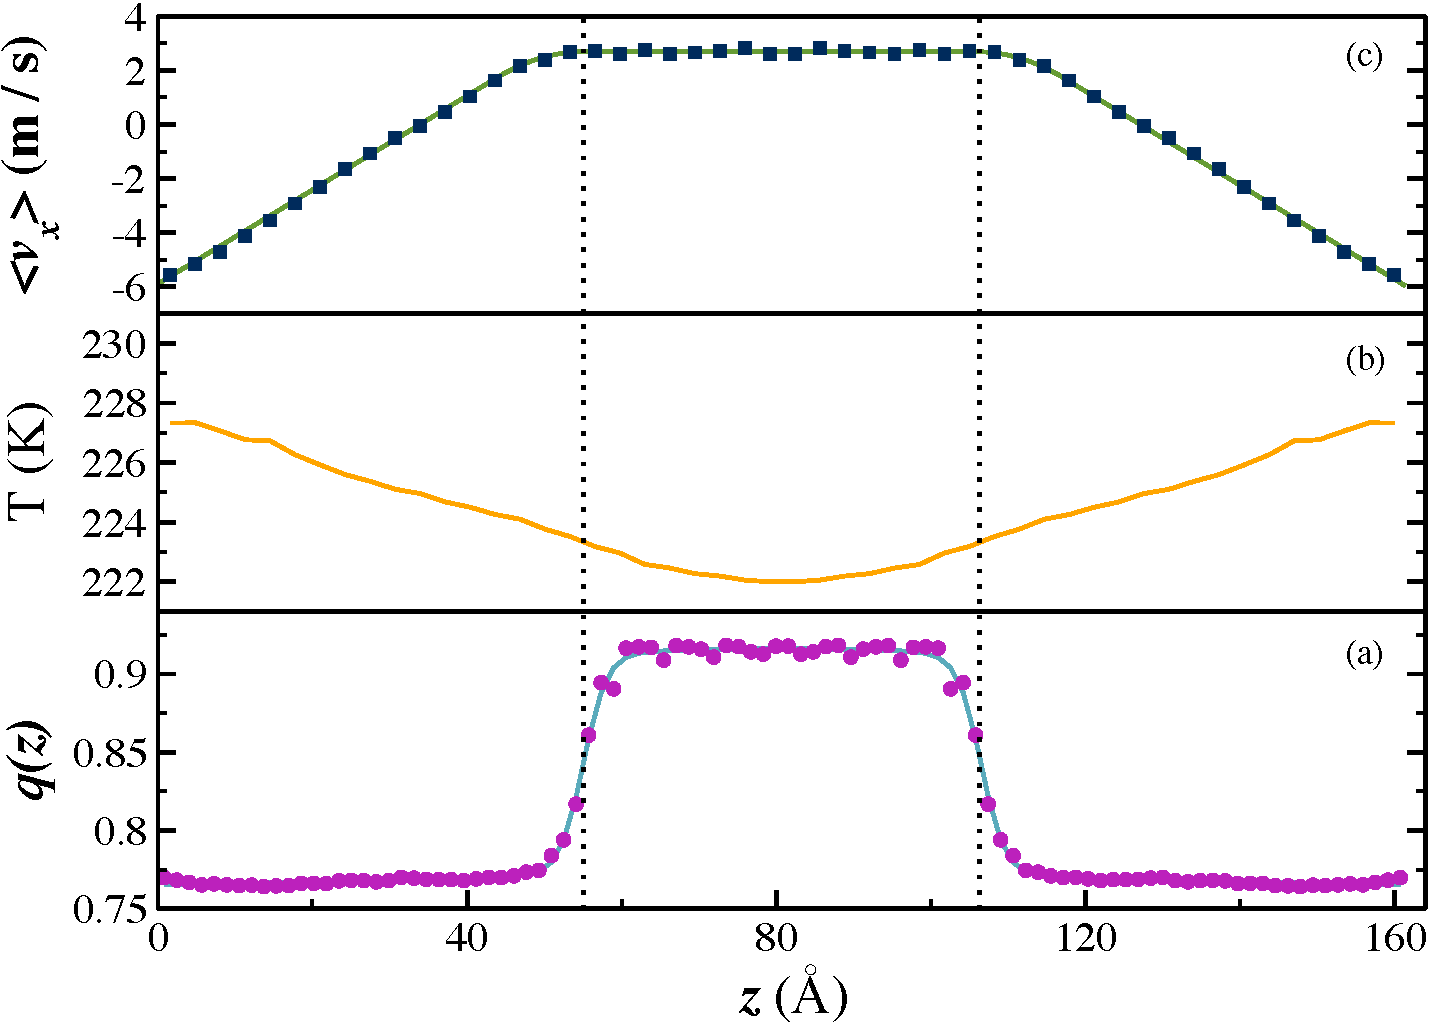
\includegraphics[width=\linewidth]{Figures/Sec_comic_strip}
\caption{\label{fig:spComic} Properties of the secondary prism
  interface being sheared through water at 8.6
  ms\textsuperscript{-1}. Lower panel: the local tetrahedral order
  parameter, $q(z)$, (circles) and the hyperbolic tangent fit
  (turquoise line).  Middle panel: the imposed thermal gradient
  required to maintain a fixed interfacial temperature of 225 K. Upper
  panel: the transverse velocity gradient (squares) that develops in
  response to an imposed momentum flux, along with the fit (green
  line). The vertical dotted lines indicate the locations of the Gibbs
  dividing surfaces of the two interfaces.}
\end{figure}

In the middle panel of Fig. \ref{fig:spComic}, we show the resulting
thermal gradient from the imposed kinetic energy flux. At the ice /
water interface, the local temperature is held at approximately 225~K, allowing
investigation of the response to the shear while maintaining
solid-liquid coexistence. In the top panel, the velocity gradient
resulting from the imposed momentum flux shows that the ice has a
uniform positive velocity along the $x$ axis. The bulk liquid at the
ends of the simulation cell has negative velocity, although the center
of mass of the simulation box is stationary.  The bulk fluid shows a
primarily linear velocity gradient allowing for easy calculation of
the shear viscosity. Close to the interface, the ice imparts
significant positive momentum into the surrounding interfacial liquid.
Projections of the velocity gradient from the liquid onto the Gibbs
dividing surface indicate that the ice-water interface is in the
negative slip regime.

From Eq. \eqref{tet_fit}, we have obtained estimates for $w$, the
structural widths of the interfaces for the quiescent ice / water
systems. These values are related to the $10\%-90\%$ interfacial
widths commonly reported in previous studies
($w_\mathrm{10-90} = 2.197~w$).\cite{Bryk2002,Bryk2004} We find
$w_\mathrm{10-90} \approx 7$~\AA~ for each of the interfaces as seen
in Table \ref{tab:kappa}.  These values are similar to our previous
findings for the $10\%-90\%$ interfacial widths obtained from shorter
simulations, ($7.0 \pm 0.9$ \AA) for the basal and ($7.9 \pm 0.4$ \AA)
for the prismatic interfaces.\cite{Louden2013} Over the range of shear
rates investigated, $\sim 0.5-10.0~\mathrm{~m~s}^{-1}$, we find no
significant differences in the interfacial widths for any of the
crystal faces. All values of $w_\mathrm{10-90}$ obtained from shearing
simulations fell inside the error bars of the values obtained from the
quiescent simulations.

\begin{table}[h]
\centering
\caption{Structural and dynamic properties of the interfaces of
  Ice-I$_\mathrm{h}$ with water.\label{tab:kappa}}
\begin{tabular}{r|cccc}  
\toprule
Interface & $w_\mathrm{10-90}$ (\AA) &  $d_\mathrm{10-90}$ (\AA) & $\kappa$ (amu \AA\textsuperscript{-2} fs\textsuperscript{-1}) & $\rho_{sl}$ (\AA\textsuperscript{-2}) \\ 
\midrule
Basal  $\{0001\}$                 & $7.5 \pm 0.4$ & $5 \pm 1$ &  $0.31 \pm 0.03$  & $0.1227 \pm 0.0003$  \\
Prismatic  $\{10\bar{1}0\}$       & $7.2 \pm 0.2$ & $8 \pm 2$  &  $0.48 \pm 0.04$  & $0.2014 \pm 0.0005$  \\
Pyramidal  $\{20\bar{2}1\}$       & $6.6 \pm 0.2$ & $6 \pm 1$ &  $0.26 \pm 0.02$  & $0.0866 \pm 0.0003$  \\
Secondary Prism  $\{11\bar{2}0\}$ & $6.7 \pm 0.2$ & $7 \pm 1$ &  $0.41 \pm 0.02$  & $0.1384 \pm 0.0004$  \\ 
\bottomrule
\end{tabular}
\end{table}

These values agree well with those reported by Haymet \textit{et
  al.}.\cite{Karim1988,Karim1990,Hayward2001,Bryk2002,Hayward2002,Bryk2004}
Using a variety of water models and several different order
parameters, they have estimated the ice / water interface to be
between $5$~\AA~and $18$~\AA~depending on the particular interface and
means of measure.  For the SPC/E model, they found the basal and
prismatic ice / water interface to be $\approx 11$~\AA~ wide from
translational and window-averaged density order parameters. The
interfacial widths were also estimated by observing the transition of
a similar tetrahedral order parameter from their ice-like value of
$0.9$ to the bulk liquid value of $0.6$. This gave estimates of
$\approx 11$~\AA~, somewhat larger than our current estimates.

\subsection{Solid-liquid friction at ice/water interfaces}
In no-stick boundary conditions, fluid flowing over a solid is
characterized by a slip length, $\delta$, describing the extent of
slip of the fluid at the interface. This length is the extrapolated
distance from the interface where the tangential velocity component
vanishes. For solids with weak interactions with the liquid, there is
little drag imposed on the fluid and the resulting interfacial liquid
velocity, $\Delta v_\mathrm{slip}$, can be significant. In no-stick
boundaries, therefore, the extrapolated slip lengths are also large
(top panel of Fig. \ref{fig:slipLengthPlot}).  Balasubramanian and
Mundy have related the slip length to the interfacial friction
coefficient, 
\begin{equation}\label{kappa1}
\lambda = \frac{\eta}{\delta}
\end{equation}
where $\eta$ is the shear viscosity of the
liquid.\cite{Balasubramanian1999}

For solids that have strong interactions with the liquid, a larger
frictional drag is imposed on the fluid at the interface and the
resulting slip lengths are smaller. When the solid-liquid interactions
become large enough, the interface is best described with stick
boundary conditions, and the slip length will vanish (middle panel of
Fig. \ref{fig:slipLengthPlot}).  Stick boundaries pose a problem for
Eq.  \eqref{kappa1}, as $\lambda$ asymptotically goes to infinity as
$\delta \rightarrow 0$.  Likewise, some materials possess solid-liquid
interactions that are strong enough for the extrapolated tangential
velocity to vanish \textit{before} reaching the solid. The velocity
profile yields a negative slip length (bottom panel of Fig.
\ref{fig:slipLengthPlot}), and the solid-liquid friction coefficient
defined in Eq. \eqref{kappa1} becomes meaningless.  Ice shearing
through liquid water is in the negative slip limit. The tangential
velocity profile of the liquid extrapolates to zero several molecular
layers before reaching the solid. Thus a new friction coefficient must
be defined to describe these interfaces.

\begin{figure}
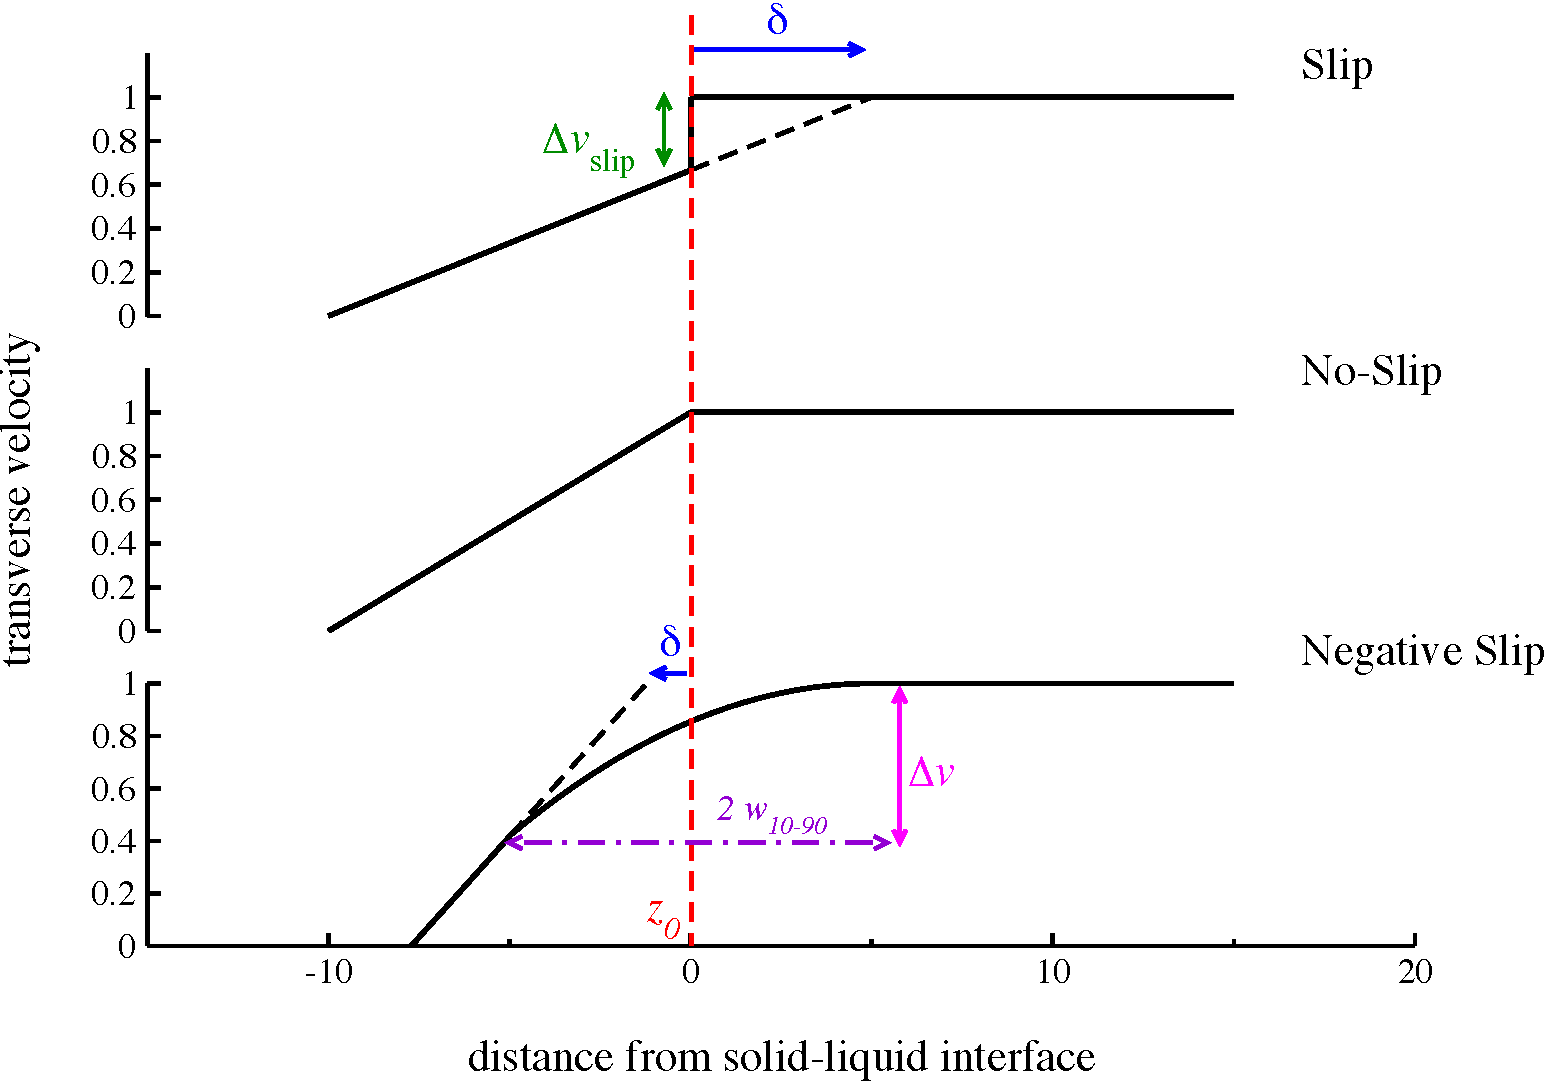
\includegraphics[width=\linewidth]{Figures/slipLengthPlot}
\caption{\label{fig:slipLength} Transverse velocity profiles,
  $v_x(z)$, for interfaces in slip (top), no-slip (middle), and
  negative slip boundary conditions (bottom).  The location of the
  interface is defined by a Gibbs dividing surface at $z_0$. Under
  negative slip conditions, the 10-90 interfacial width, $w_{10-90}$,
  provides locations that are unambiguously on the liquid and solid
  sides of the interface.\label{fig:slipLengthPlot}}
\end{figure}

The solid-liquid friction coefficient may also be defined using the
velocity drop across the interface, rather than the length scale over
which this drop occurs. We can relate the imposed shear stress with
the relative tangential velocity of the fluid in the interfacial
region,\cite{Kuang2012}
\begin{equation}\label{Shenyu-13}
j_{z}(p_{x}) = \kappa \Delta v
\end{equation}
where $\Delta v = v_{x}(\mathrm{solid}) - v_{x}(\mathrm{liquid})$ is
the difference in transverse velocity between points that are
unambiguously on the solid and liquid sides of the interface.  In slip
boundary conditions, $\kappa$ and $\lambda$ are identical, but
Eq. \eqref{Shenyu-13} provides a direct analogy to non-equilibrium
expressions for the interfacial thermal conductance $(G)$,
\begin{equation}
J_z = G~ \Delta T.
\end{equation}
Here, $J_z$ is a thermal flux and the temperature drop is measured
across an interface of \textit{finite width}. By analogy, $\kappa$ is
a transport coefficient that measures interfacial momentum
conductance.

In ice/water interfaces, the solid-liquid boundary is not
an infinitely thin plane. An order parameter (the tetrahedrality) goes
smoothly between the phases over a few molecular diameters.  We can
use this order parameter to find the interfacial width and define
locations in space that are unambiguously on the solid and liquid
sides of the interface.  In what follows, we have used the Gibbs
dividing surface ($z_0$) and the 10$-$90 width of the interface
($w_\mathrm{10-90}$) to arrive at physical locations for measuring
$v_{x}(solid)$ and $v_{x}(liquid)$.  These uniquely define a friction
coefficient in terms of well-defined structural features ($z_0$ and
$w_\mathrm{10-90}$) and dynamic properties ($v_{x}(z)$) of the
interface.

Tangential velocity profiles from the simulations were fit using a
piecewise function that is both continuous and continuously
differentiable (see Supporting Information). To arrive at estimates of
the interfacial velocities, these fits were queried at locations on
either side of the structural Gibbs dividing surface,
\begin{align*}
v_{x}(\mathrm{solid}) & = v_{x}( z_0 + w_\mathrm{10-90}) \\
v_{x}(\mathrm{liquid}) & = v_{x}( z_0 - w_\mathrm{10-90}).
\end{align*}
The momentum flux, $j_{z}(p_{x})$ is an imposed parameter of the
VSS-RNEMD simulations, and by using Eq. \eqref{Shenyu-13}, estimates
of interfacial friction coefficient $\kappa$ are straightforward.

The calculated $\kappa$ values found for the four crystalline facets
of ice-I$_\mathrm{h}$ investigated here are shown in Table
\ref{tab:kappa}.  These results were found to be independent of the
shear rate, as well as the direction of the shear relative to the
features on the surfaces of the facets.

Note that the values of $\kappa$ for the basal and prismatic crystal
facets in Table \ref{tab:kappa} disagree with values for interfacial
friction ($\lambda$) we previously reported.\cite{Louden2013} In our
initial report, the expression for the coefficient of friction was
derived from equation \eqref{kappa1} and the linear constitutive
relation for shear stress in a bulk fluid.  However, as described
above, sheared ice/water interfaces are in the domain negative slip
lengths. Eq. \eqref{kappa1} should only be used in slip boundary
conditions, as negative slip can yield coefficients of friction that
appear to be smaller in magnitude than the zero slip conditions. In
our previous work, the prismatic surface was found to have a larger
negative slip length than the basal face, indicating a prismatic
surface that should have been reported with a larger coefficient of
friction. If one instead uses Eq. \eqref{Shenyu-13} and interfacial
widths to compute friction, the reported values come into agreement.

\subsection{Dynamic measures of interfacial width under shear}
The spatially-resolved orientational time correlation function,
\begin{equation}\label{C(t)1}
  C_{2}(z,t)=\langle P_{2}(\mathbf{u}_i(0)\cdot \mathbf{u}_i(t))
  \delta(z_i(0) - z) \rangle,
\end{equation}
provides local information about the decorrelation of molecular
orientations in time. Here, $P_{2}$ is the second-order Legendre
polynomial, and $\mathbf{u}_i$ is the molecular unit vector that bisects
the HOH angle of molecule $i$. The angle brackets indicate an average
over all the water molecules and time origins, and the delta function
restricts the average to specific regions in the $z$-dimension. 

Recently, Laage and Hynes have determined the mechanism for water
reorientation.\cite{Laage2006,Laage2008} Using molecular dynamics
simulations, they found that water reorients by breaking a hydrogen
bond with an overcoordinated first-shell neighbor, and makes a large
angle jump to form a new hydrogen bond with an undercoordinated
second-shell neighbor.  The hydrogen bond cleavage and molecular
reorientation occur in a concerted fashion, not in successive steps as
was previously thought.  With this detailed picture, they constructed
the Extended Jump Model\cite{Laage2006,Laage2008} based on the Ivanov
Jump Model and parameters extracted from their molecular simulations;
the average jump amplitude of the rotational jump, $\theta_{0}$, and
the frequency of the jumps, $1/\tau_{0}$. After accounting for
molecular frame reorientation, the Extended Jump Model is able to
predict reorientation relaxation times, $\tau_{n}^{jump}$, which agree
with experimental results as well as estimates obtained from
simulations where fast librational motion is ignored.

In the ice crystal, decay of $C_2(z,t)$ is incomplete, while in the
liquid, correlation times are typically measured in ps. Observing the
spatial-transition between the decay regimes can define a dynamic
measure of the interfacial width.  To determine the dynamic widths of
the interfaces under shear, each of the systems were divided into bins
along the $z$ axis ($\approx$ 1 \AA\ wide) and $C_2(z,t)$ was computed
using only those molecules that were in the bin at the initial
time. For each ice / water interface investigated, the following 0.5
ns simulations were computed: quiescent simulations (where no thermal
or momentum gradient was present), simulations with only a thermal
gradient present, and simulations where both thermal and momentum
gradients were present. During these simulations, the positions and
orientations of each molecule were recorded every 100 fs.

\begin{figure}
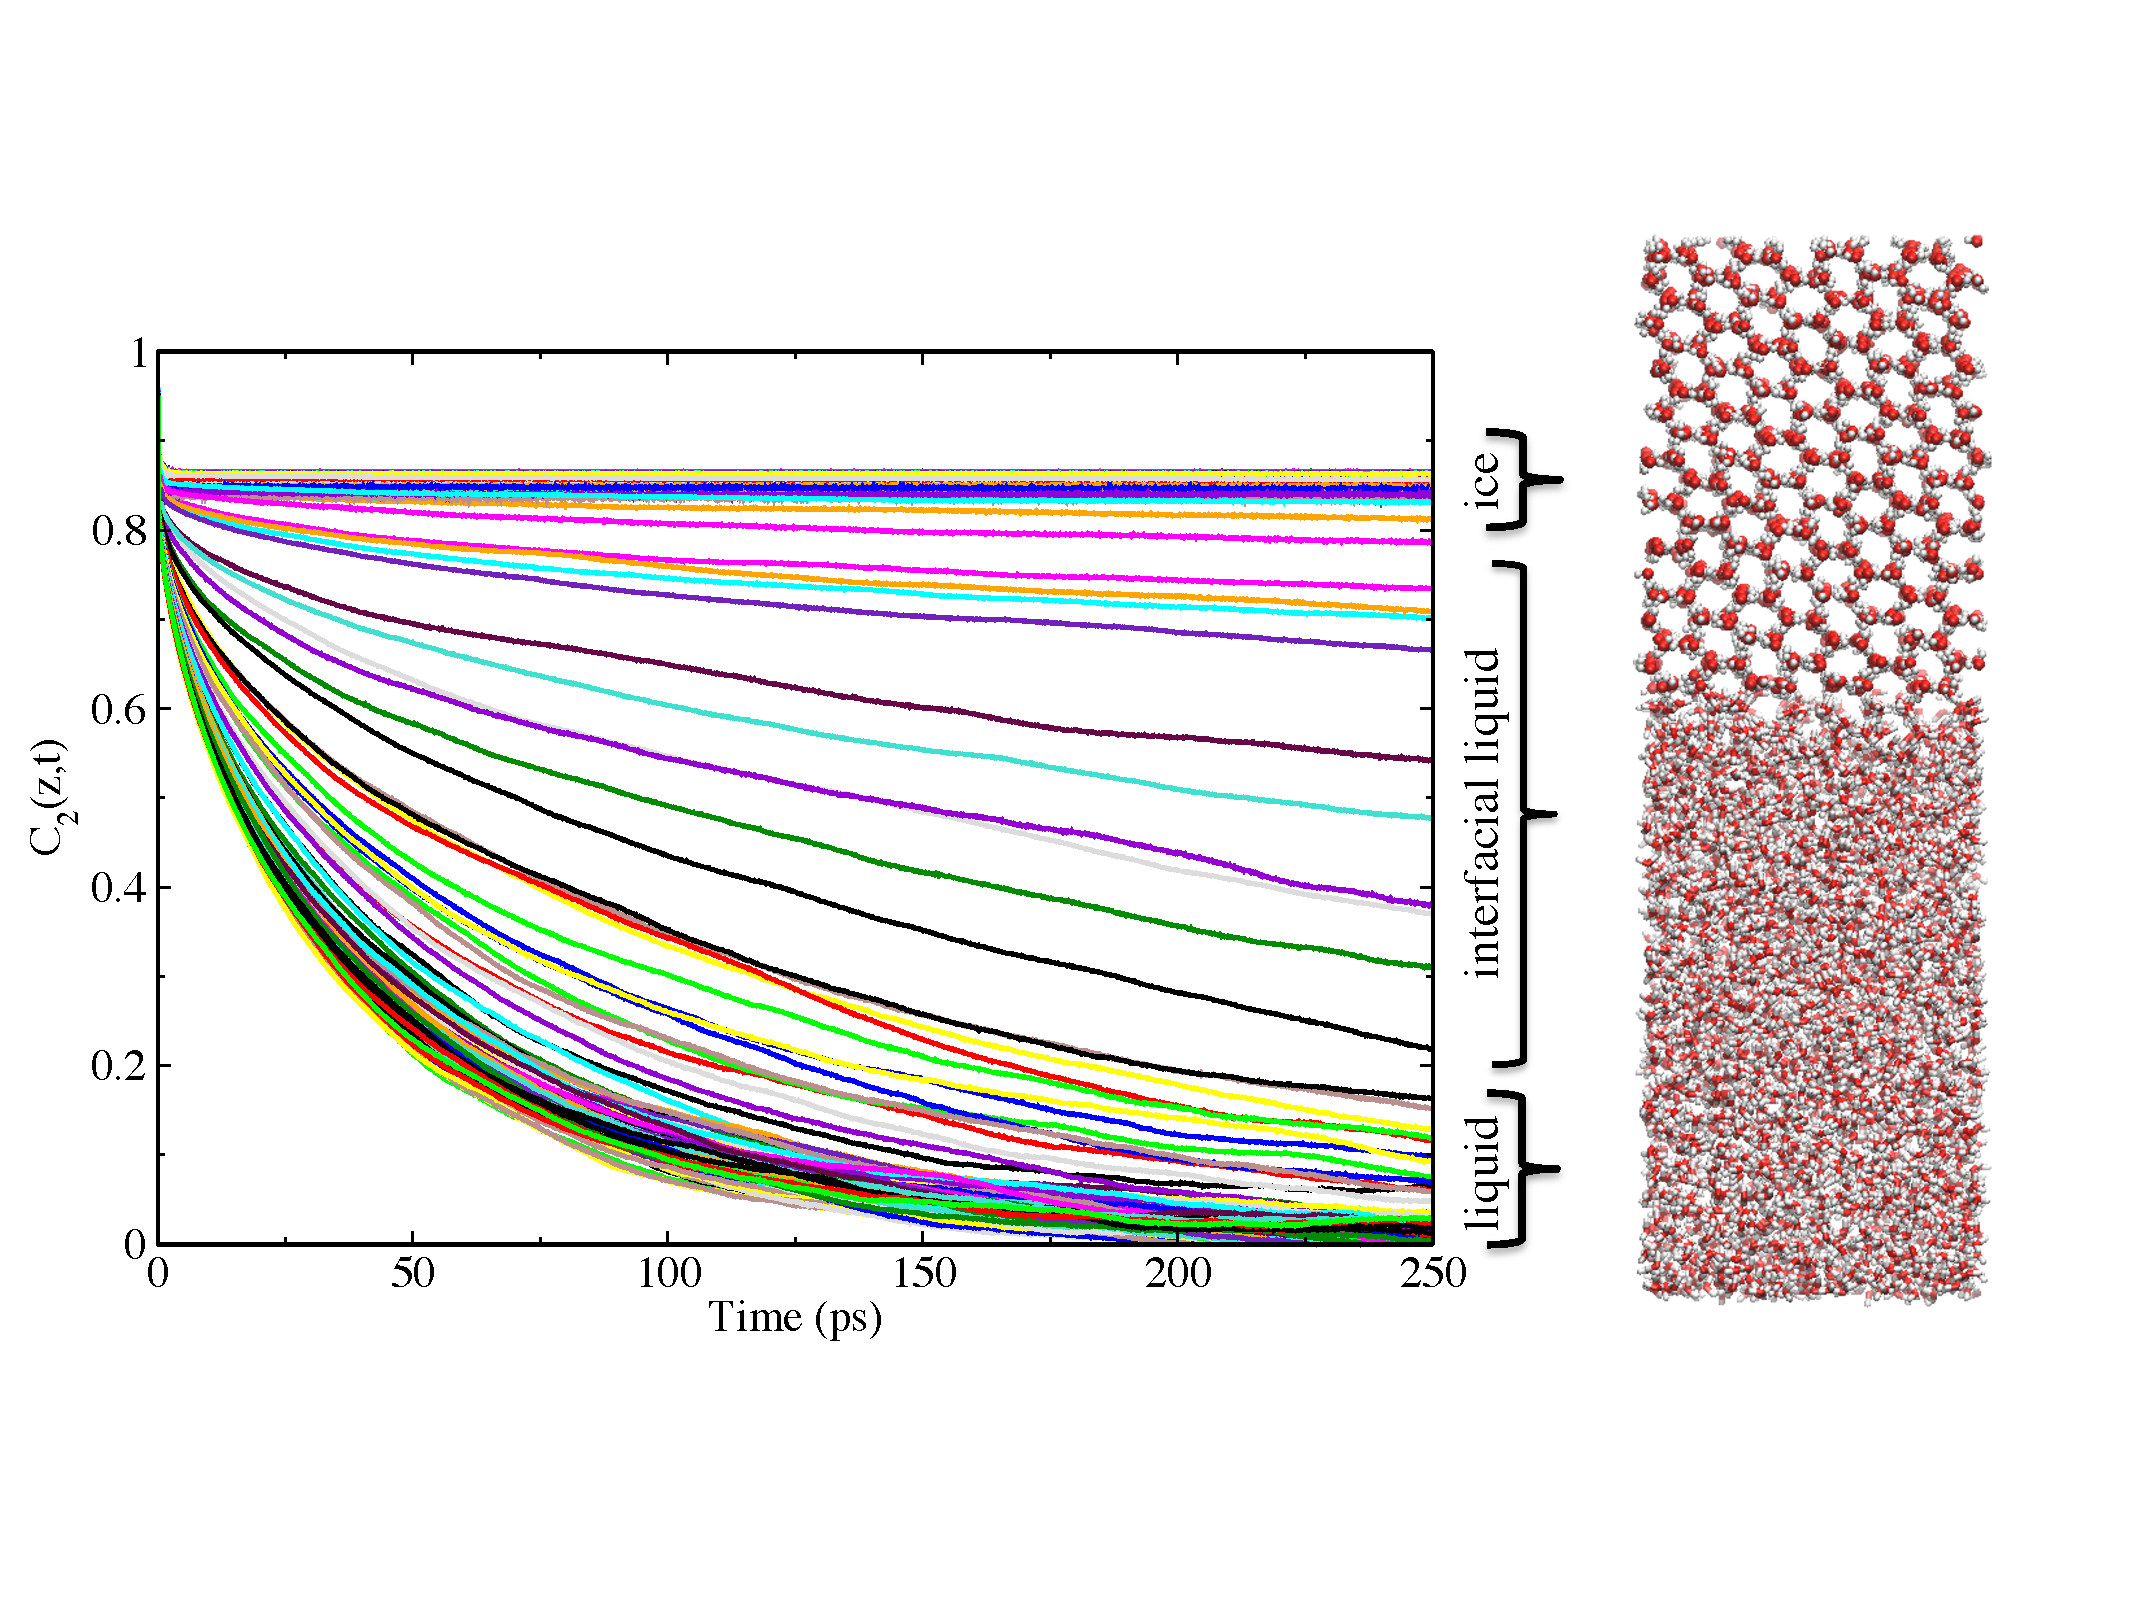
\includegraphics[width=\linewidth]{Figures/CztImage}
\caption{\label{fig:Czt} $C_2(z,t)$ collected in 1 \AA~bins across the
  secondary prism ice/water interface. The band that experiences very
  little decay represents water molecules in the ice, while the band
  that decays quickly corresponds to bins in the liquid.  The
  correlation function presents a continuous distribution of decay
  behaviors across the interface between ice and liquid water.}
\end{figure}

Computed $C_2(z,t)$ values have previously been fit to a
triexponential decay, with three time constants:
$\tau_\mathrm{short}$, measuring the librational motion of the water
molecules, $\tau_\mathrm{middle}$, measuring the timescale for the
large angle jumps during the breaking and making of hydrogen bonds,
and $\tau_\mathrm{long}$, corresponding to the translational motion of
the water molecules.\cite{Louden2013} The Extended Jump Model also
includes three similar decay constants, however two of them are linked
and the dynamics of the decay is governed by two parameters. Since we
are interested in how the decay times and the individual contributions
may change through the interface, we have fit the $C_2(z,t)$ data
with
\begin{equation}
  C_{2}(z,t) = a~e^{-t/\tau_\mathrm{short}} + b~e^{-t/\tau_\mathrm{middle}} + 
  (1-a-b)~e^{-t/\tau_\mathrm{long}}
\label{eq:c2}
\end{equation}
where all of the decay constants are considered local functions of the
$z$ coordinate. In Fig. \ref{fig:SPorient}, the $z$-coordinate
profiles for the three decay constants, $\tau_{\mathrm{short}}$,
$\tau_{\mathrm{middle}}$, and $\tau_{\mathrm{long}}$ for the secondary prism interface
is shown, along with their fractional components of the overall total
decay, ($a$, $b$, $1-a-b$), respectively. Similar figures for the
other interfaces are provided in the Supporting Information.

In the liquid regions of all four interfaces, $\tau_\mathrm{middle}$
and $\tau_\mathrm{long}$ consistently approach $3-6$ ps and $30-40$
ps, respectively.  Both of these times increase closer to the
interface.  Conversely, $\tau_\mathrm{short}$ decreases from a
liquid-state value of $72-76$ fs approaching the interface.

The fractional contributions of the three motions to the overall decay
changes as we approach the interface as well. Far from the ice, the
librational motion and hydrogen bond breaking/making events each
contribute to about 20 percent of the total decay, whereas frame
reorientation contributes about 60 percent. As we approach the
interface, the librations and hydrogen bond dynamics both decrease in
contribution. The librations comprise approximately 15 percent of the
overall decay at the edge of the interface, whereas the hydrogen bond
contributions drop to approximately zero. In contrast, the fraction of
the total decay due to frame reorientation is shown to increase
approaching the interface.  The time constant corresponding to this
motion is seen to logarithmically increase as we approach the interface
as the molecules become more ice-like. In the ice we would expect
molecular reorientation to be incomplete, however, at the interface we
observe frame reorientation to contribute 85 percent of the overall
decay.

\newpage
\begin{figure}
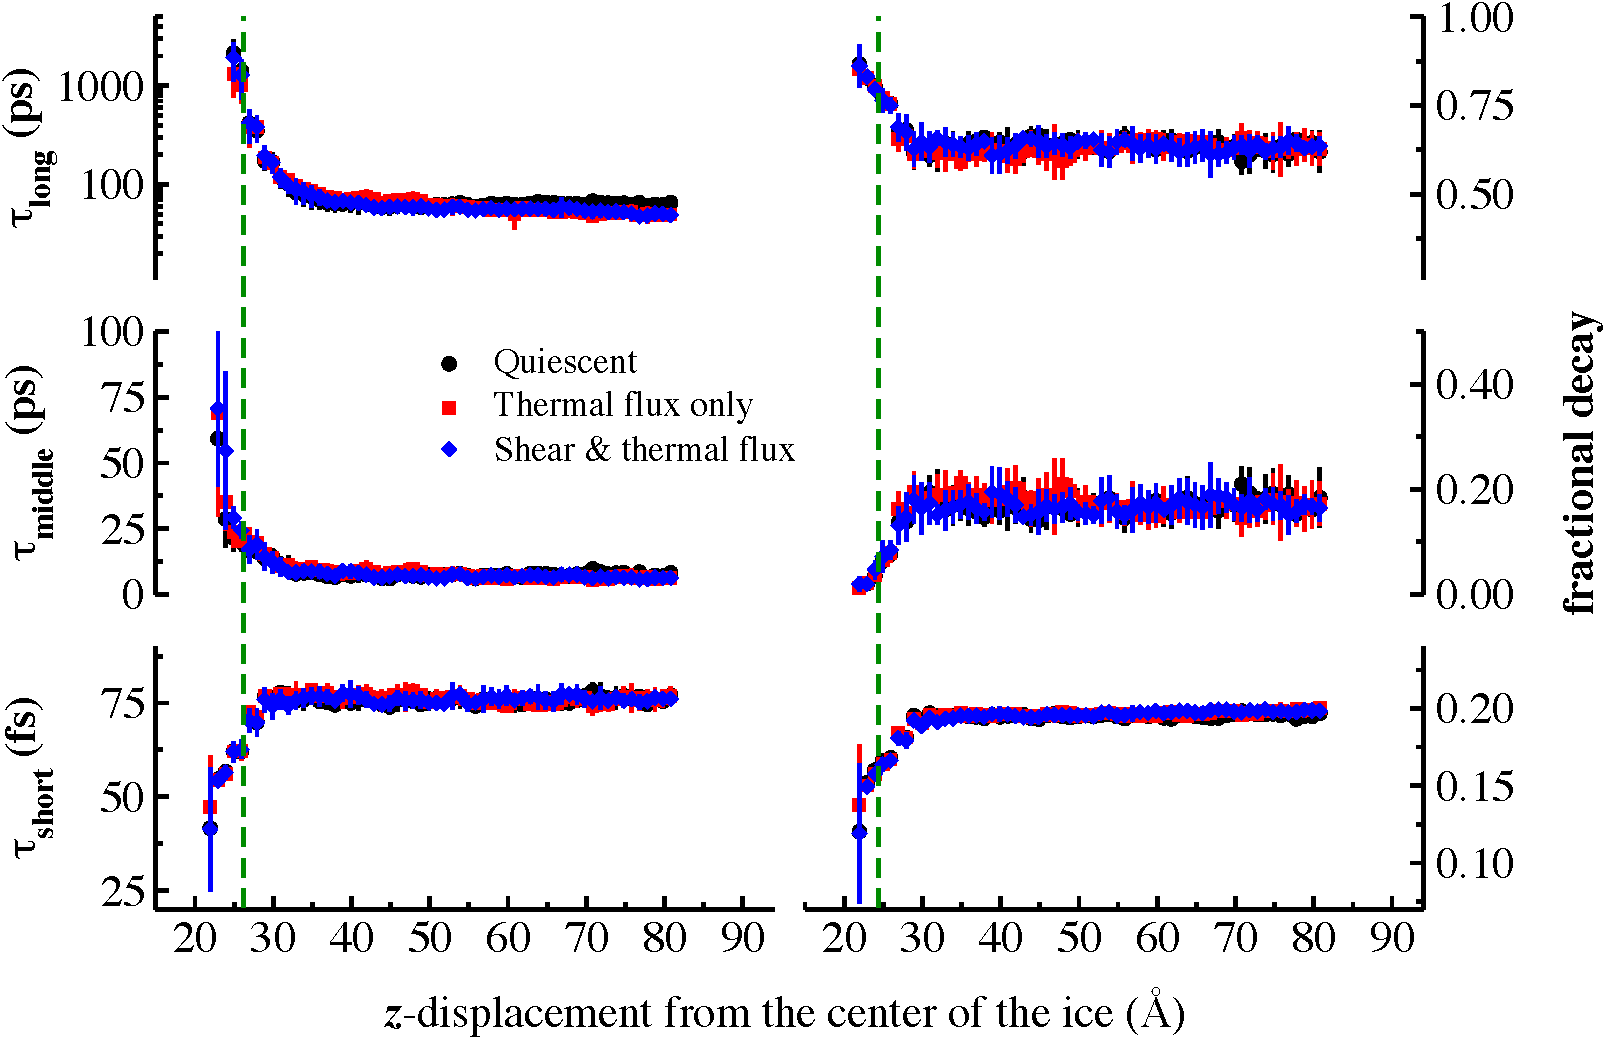
\includegraphics[width=\linewidth]{Figures/Sec_lcorrz}
\caption{\label{fig:SPorient} Decay times (left) for $C_2(z,t)$ at the
  secondary prism interface, and their fractional contributions to the
  overall decay (right) fit using Eq. \eqref{eq:c2}. The local decay
  constants are plotted as a function of distance from the center of
  the ice slab. The vertical dashed line indicates the Gibbs dividing
  surface determined using the local tetrahedral order parameter.
  Results are shown for a quiescent system with no applied kinetic or
  momentum flux (black), an interface with an imposed
  kinetic energy flux (red), and a sheared simulation (blue) with both
  kinetic and momentum fluxes.}
\end{figure}

We have estimated a dynamic interfacial width by fitting the profiles
of all the three orientational time constants with an exponential
decay to the bulk-liquid behavior,
\begin{equation}\label{tauFit}
  \tau(z) = \tau_\mathrm{liquid}+(\tau_\mathrm{wall}-\tau_\mathrm{liquid})e^{-(z-z_{0})/d}
\end{equation}
where $\tau_\mathrm{liquid}$ and $\tau_\mathrm{wall}$ are the liquid
and projected interfacial values of the decay constants, $z_{0}$ is
the location of the Gibbs dividing surface, as measured by the
structural order parameter.  As with the structural widths,
$10\%-90\%$ dynamic widths are easily computed from the fits
($d_\mathrm{10-90} = 2.197~d$).  These values are provided in Table
\ref{tab:kappa}. All four interfaces exhibit dynamic widths that are
$\sim 6$~\AA, and are in reasonable agreement with the structural
widths above.

We note that Bryk and Haymet also calculated the orientational time
correlation function at the basal interface of SPC/E
water,\cite{Bryk2002} and observed the same qualitative trend through
the ice / water interface, although the spatial resolution was not
sufficient to resolve a dynamic width.
 
Laage and Hynes investigated how water molecules reorient around
ions\cite{Laage2007,Laage2008a,Stirnemann2011a,Laage2011},
proteins\cite{Duboue-Dijon2014}, and in confined
spaces\cite{Laage2012b,Fogarty2014}.  They also studied how the
strength of the hydrogen bond might perturb the reorientation
dynamics,\cite{Laage2006a} and found the librational motion which
forms a cone around the O-O vector is smaller for more strongly
hydrogen bonded water This may also provide a partial explanation for
the increasing contribution of short time decay very close to the ice
surfaces.  Since the solid creates an excluded volume for the water
molecules that are in proximity to the interface, the hindered range
of motion (i.e., a smaller cone around the O-O vector) manifests as
faster librational decay.

\section{Discussion}
The primary result of this paper is the observation that the different
facets of ice-I$_\mathrm{h}$ produce significantly different
solid-liquid interfacial friction coefficients with water (see Table
\ref{tab:kappa}).  The two prismatic surfaces displayed the largest
coefficients of friction, while the basal and pyramidal facets
exhibited significantly lower friction.

The differences in friction are surprising given that densities and
molecular interactions are identical for the four interfaces and the
interfacial widths measured via both structural and dynamic features
are also nearly the same. There are few remaining surface properties
that could give rise to differences in solid-liquid friction of the
four facets, notably surface corrugation and hydrogen bonding density
at the interface. In this section we investigate the roles of these
surface features.

\subsubsection{Solid-liquid hydrogen bond density}
One reason for the observed differences in friction
coefficients is that ice surfaces may yield different densities of
hydrogen bonds that bridge the solid and liquid.  An ice surface that
forms more hydrogen bonds with the interfacial liquid would be able to
exert significant lateral forces on the liquid layer, yielding a
larger friction coefficient. To probe this possibility, we have
investigated the density of cross hydrogen bonds between the ice and
the liquid.

Quantifying water molecules as ``ice'' or ``liquid'' at an interface
of finite width requires a local order parameter for separating the
molecules.  We have again chosen the tetrahedral order parameter, $q$
and the value of at the Gibbs dividing surface $(q(z_0) \approx 0.84)$
as our partitioning criterion.  Note that some molecules have strong
tetrahedral ordering in the liquid phase, so this segregation will not
yield perfect division between ice and liquid phase molecules.

To determine if a hydrogen bond has been formed between two water
molecules, we used the geometric criteria of Luzar and
Chandler.\cite{Luzar1996} We identify a hydrogen bond between two
water molecules if their oxygen sites are within $r_{OO} < 3.5$
\AA~and the OHO bond angle is within $\theta_{OHO} < 30$ degrees.

For each of the shearing simulations performed above, a hydrogen bond
tetrahedrality matrix was constructed.  Snapshots from the shearing
trajectories were taken every $0.1$ ps, and the tetrahedrality $(q)$
value for each water molecule in the system was calculated. Hydrogen
bonds were also identified, and the tetrahedrality of the donor
$(q_{D})$ and acceptor $(q_{A})$ molecules were recorded. A
probability density of hydrogen bonds categorized by donor and
acceptor tetrahedrality, $\rho_\mathrm{HB}(q_D, q_A)$, was then
recorded.

\newpage
\begin{figure}
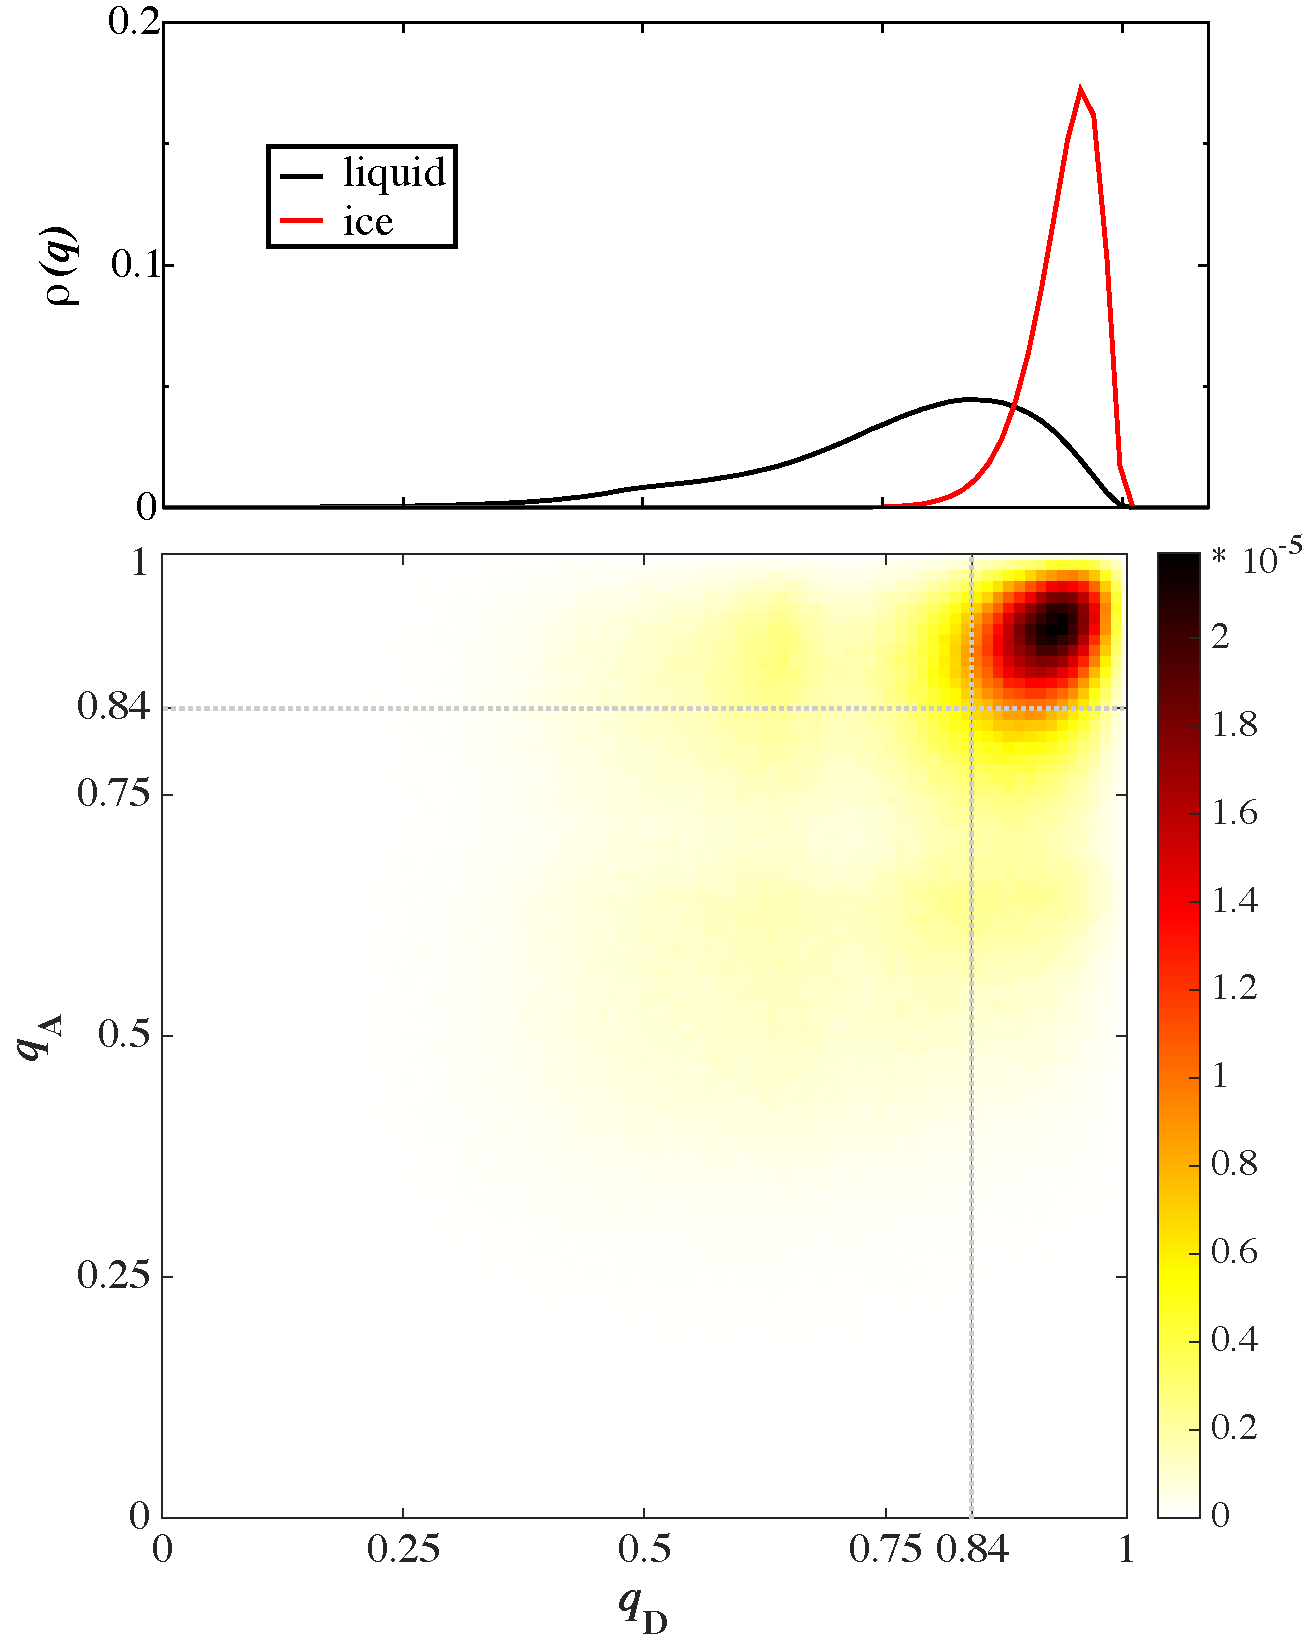
\includegraphics[width=5in]{Figures/hbtet.pdf}
\caption{\label{fig:tetHBMatrix} Distribution of hydrogen bonds at a
  prismatic interface showing the tetrahedralities of donor $(q_D)$
  and acceptor $(q_A)$ molecules (lower panel). Distributions of
  tetrahedralities in bulk ice and liquid phases are shown in the
  upper panel, and the value of $q$ at the Gibbs dividing surface is
  indicated with dashed lines. Hydrogen bonds between ice molecules
  are represented by the upper right square, while those between
  liquid molecules are in the lower left.  Hydrogen bonds that bridge
  the ice-liquid interface exist primarily in the vertical and
  horizontal strips that remain.}
\end{figure}


The lower panel of Fig. \ref{fig:tetHBMatrix} shows a hydrogen bond
tetrahedrality distribution for the prismatic facet with $q_{D}$
plotted along the $x$-axis and $q_{A}$ along the $y$-axis.  Population
around $q_{D} \approx q_{A} \approx 0.9$ indicates the density of
ice-ice hydrogen bonds in the system, while the liquid-state hydrogen
bonds are concentrated in the lower left, and are significantly more
diffuse.  The off-diagonal regions of the distribution represent the
population of molecules in tetrahedral (ice-like) environments bound
to non-tetrahedral (liquid-like) environments. Integrating the
population found in each of these regions and normalizing by the
surface area of each ice crystal produces a surface density of
hydrogen bonds (\AA\textsuperscript{-2}) formed between the ice and
interfacial liquid,
\begin{equation}\label{hbondDensity}
\rho_{sl} = \frac{N_\mathrm{HB}}{2 L_{x}L_{y}} \left[ \int_0^{0.84}
  dq_{D} \int_{0.84}^1 dq_{A}~\rho_\mathrm{HB}(q_{D},q_{A}) +  \int_0^{0.84}
  dq_{A} \int_{0.84}^1 dq_{D}~\rho_\mathrm{HB}(q_{D},q_{A}) \right]
\end{equation}
$N_\mathrm{HB}$ is the total number of hydrogen bonds found in the
system, and $L_x$ and $L_y$ are the dimensions of the two ice facets
exposed to the liquid.  Values for $\rho_{sl}$ for each of the ice
surfaces are reported in Table \ref{tab:kappa}.

The trend in surface density of solid-liquid hydrogen bonds reproduces
the trend in the friction coefficients, indicating that friction at
ice-I$_\mathrm{h}$ water interfaces is strongly influenced, if not
governed, by the number of solid-liquid hydrogen bonds that can be
formed.  This result is robust under multiple shear rates and
orientation of shear flow relative to the surface features of the ice,
indicating that the hydrogen bonding statistics between an ice facet
and the liquid are not altered by the imposed shear.

\subsubsection{Surface corrugation}
A second possible influence on the friction coefficient is the surface
topography of the ice crystals, the dimensions of which are reported
in Table \ref{tab:surf}. When a crystal of ice-I$_\mathrm{h}$ is
cleaved along either of the two prismatic crystal facets, the exposed
oxygen atoms present channel-like structures with channel widths of
6.35~\AA~ and channel depths of 2.25~\AA~.  When cleaved along the
pyramidal facet, the resulting surface features a much larger channel,
$\sim$ 8.7~\AA~ wide.  Conversely, the basal surface presents a
rather smooth surface to the liquid, with stripes of oxygen atoms
forming surface ripples with depths of $\sim$ 1.3~\AA~.

\begin{table}[h]
\centering
\caption{Surface features of Ice-I$_\mathrm{h}$ facets.\label{tab:surf}}
\begin{tabular}{r|cc}  
\toprule
Interface & Channel width (\AA) & Channel depth (\AA) \\ 
\midrule
Basal  $\{0001\}$                 & 4.49 & 1.30 \\
Prismatic  $\{10\bar{1}0\}$       & 6.35 & 2.25 \\
Pyramidal  $\{20\bar{2}1\}$       & 8.65 & 2.59 \\
Secondary Prism  $\{11\bar{2}0\}$ & 6.35 & 2.25 \\ 
\bottomrule
\end{tabular}
\end{table}

The prismatic channels are quite stable. That is, we do not observe
liquid phase molecules populating the prismatic and secondary prism
surface channels. One might expect regions of low liquid density to
yield smaller solid-liquid interactions, and it does appear that these
two surfaces present roughly half of the surface oxygen atoms to the
liquid.  However, the molecules forming the bottoms of the channels
are fully saturated (four hydrogen bonds each), while the molecules
that form the tops of the channels present a high density of available
hydrogen bond locations.

The oxygen-based surface features of the prism and secondary prism are
identical, and only the orientation of the water molecules varies.
This means that the patterning of donor and acceptors on the two
facets is quite different. A liquid with internal hydrogen bonding
constraints that is in contact with these facets will allow the
prismatic surface to form a higher density of solid-liquid hydrogen
bonds than the secondary prism, even with identical oxygen ordering at
the interface.

In contrast with the prismatic facets, liquid state molecules do
populate the surface channels on the pyramidal facet. Again, one might
expect the interactions between the solid and the liquid in close
physical contact to be quite large.  However, the liquid molecules
populating this channel do not pack efficiently and cannot fully
saturate the surface locations available for hydrogen bonding,
resulting in a lower solid-liquid hydrogen bond density and a smaller
coefficient of friction.

With its smooth surface, one could make reasonable physical arguments
for the basal face to have either high or low friction with liquid
water. That is, liquid molecules should be able to form a fully
populated network of hydrogen bonds with the surface, as there are no
recessed surface molecules at the bottoms of deep channels, and no
channel packing constraints. In the absence of large surface
undulations, however, liquid-phase molecules should also be able to
slip over the surface easily. However, the basal facet was found to
have an intermediate friction coefficient compared with the other
facets studied here. The sensible explanation in light of the
hydrogen bonding data is simply that the surface density of
solid-liquid hydrogen bonds (however transitory) dominates the
interfacial friction.

\section{Conclusions}
RNEMD simulations of the different facets of ice being drawn through
surrounding water at the coexistence temperature indicate some
facet-dependence of solid-liquid friction.  We have defined a negative
slip interfacial friction coefficient, $\kappa$ (measured in
amu~\AA$^{-2}$ fs$^{-1}$) and find that the two prismatic facets exert
the largest drag on the surrounding liquid.  The basal facet provides
an intermediate level of drag, while the pyramidal facet has roughly
half the interfacial friction of the prismatic facet.

Using the local tetrahedral order parameter as a metric to
differentiate ice and liquid water molecules and a geometric hydrogen
bonding criteria, the friction coefficients were shown to be largely
governed by the surface density of solid-liquid hydrogen bonds
($\rho_{sl}$).  A simple linear fit for the four interfaces yields
\begin{equation}
\kappa \approx 2.1772 \mathrm{(amu~fs^{-1})} \times \rho_{sl} \mathrm{(\AA^{-2})}  + 0.0777 \mathrm{(amu~\AA^{-2}~fs^{-1})},
\end{equation}
so the majority of the calculated solid-liquid friction is determined
by the surface density of solid-liquid hydrogen bonds.

In addition, we have found the ice / water interfacial widths for all
four crystal facets to be similar (using both structural and dynamic
measures) and found these widths to be independent of shear rate.  The
similarity of interfacial width estimates for the four facets indicate
that the particular facet of the exposed ice crystal has very little
effect on how far into the bulk the ice-like structural ordering
persists.  While differences have been found in previous simulations
of ice / water interfaces\cite{Hayward2001,Hayward2002},
experimentally these differences have been less
clear.\cite{Beaglehole1993} The significant differential friction
coefficients obtained here suggest that while the liquid next to the
ice might be structurally organized like bulk liquid, the dynamics of
the molecules are still quite strongly perturbed by the ice.  That is,
the surface hydrogen bonding significantly alters how the water layers
are pulled along with the ice during shear.



\section{Fitting velocity profiles}
%%%%% All this goes in SI:
In order to calculate solid-liquid friction coefficients, $\kappa$
from Eq. (5) in the main text, the velocity profiles, $v_x(z)$,
obtained from each shearing simulation were fit assuming linear
behavior through each of the three regions of the simulation box; the
lower liquid, the solid, and the upper liquid. Parabolic functions
were designed to capture the negative slip behavior that links the
three regions,
\begin{equation}\label{vfit}
v(z) =
\begin{cases}
  v_{l} - m_{l}z & 0 \leq z < (z_{1} - w) \\
  v_{s} - \frac{1}{2}k(z-z_{1})^{2} & (z_{1}-w) \leq z < z_{1} \\
  v_{s}  & z_{1} \leq z < z_{2} \\
  v_{s} - \frac{1}{2}k(z-z_{2})^{2}  & z_{2} \leq z <( z_{2} + w)\\
  v_{s} - \frac{1}{2}kw^{2} - m_{l}(z-(z_{2} + w)) & (z_{2} + w) \leq z \\
\end{cases}
\end{equation}
  
Here, $v_{l}$ is the velocity of the liquid at the middle of the
liquid domain (the edge of the simulation box), and $v_{s}$ is the
velocity of the solid. The locations $z_{1}$ and $z_{2}$ are the edges
of the ice slab, and $w$ is the width of the interface (distinct from
$w_{10-90}$ mentioned in the main text). The parameter $m_{l}$ is the
slope of the velocity profile in the liquid regions of the box which
is related to the liquid-state viscosity. Figure \ref{fig:pyrComic}
shows a representative velocity profile (navy squares) and fit (green
line) with the locations of $z_{1}$ and $z_{2}$ indicated as vertical
dotted lines. Once the fits were obtained, the values for
$v_{x}(solid)$ and $v_{x}(liquid)$ for Eq. (5) were sampled from the
fit. The $z$ locations used to sample the fit were determined by
structural measures. The $z$ location for $v_{x}(liquid)$ was taken to
be the Gibbs dividing surface of the interface, less the 10$-$90 width
of the interface. Similarly, the $z$ location for $v_{x}(solid)$ was
taken to be the Gibbs dividing surface plus the 10$-$90 width of the
interface.

%The following 4 figures are the z-rnemd profiles a. q(z), b. T(z), c. Px(z)      \newpage 
\begin{figure}
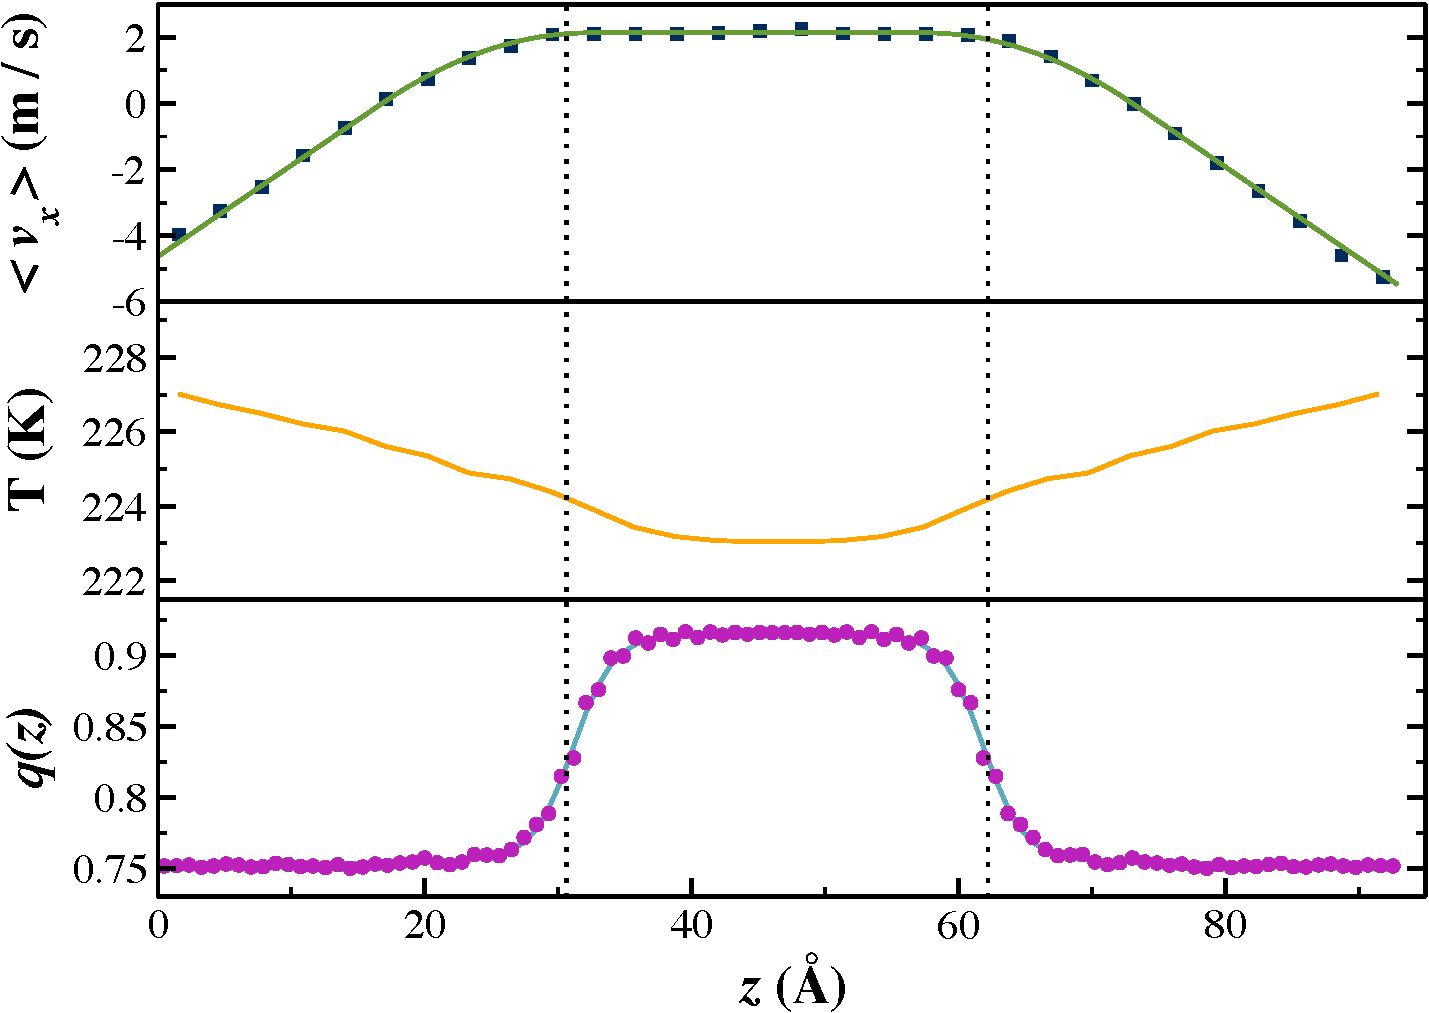
\includegraphics[width=\linewidth]{Figures/Pyr_comic_strip}
\caption{\label{fig:pyrComic} Properties of the pyramidal
  interface being sheared through water at 7.6
  ms\textsuperscript{-1}. Lower panel: the local tetrahedral order
  parameter, $q(z)$, (circles) and the hyperbolic tangent fit
  (turquoise line).  Middle panel: the imposed thermal gradient
  required to maintain a fixed interfacial temperature of 225 K. Upper
  panel: the transverse velocity gradient (squares) that develops in
  response to an imposed momentum flux, along with the fit (green
  line). The vertical dotted lines indicate the locations of the Gibbs
  dividing surfaces of the two interfaces.}
\end{figure}

\begin{figure}
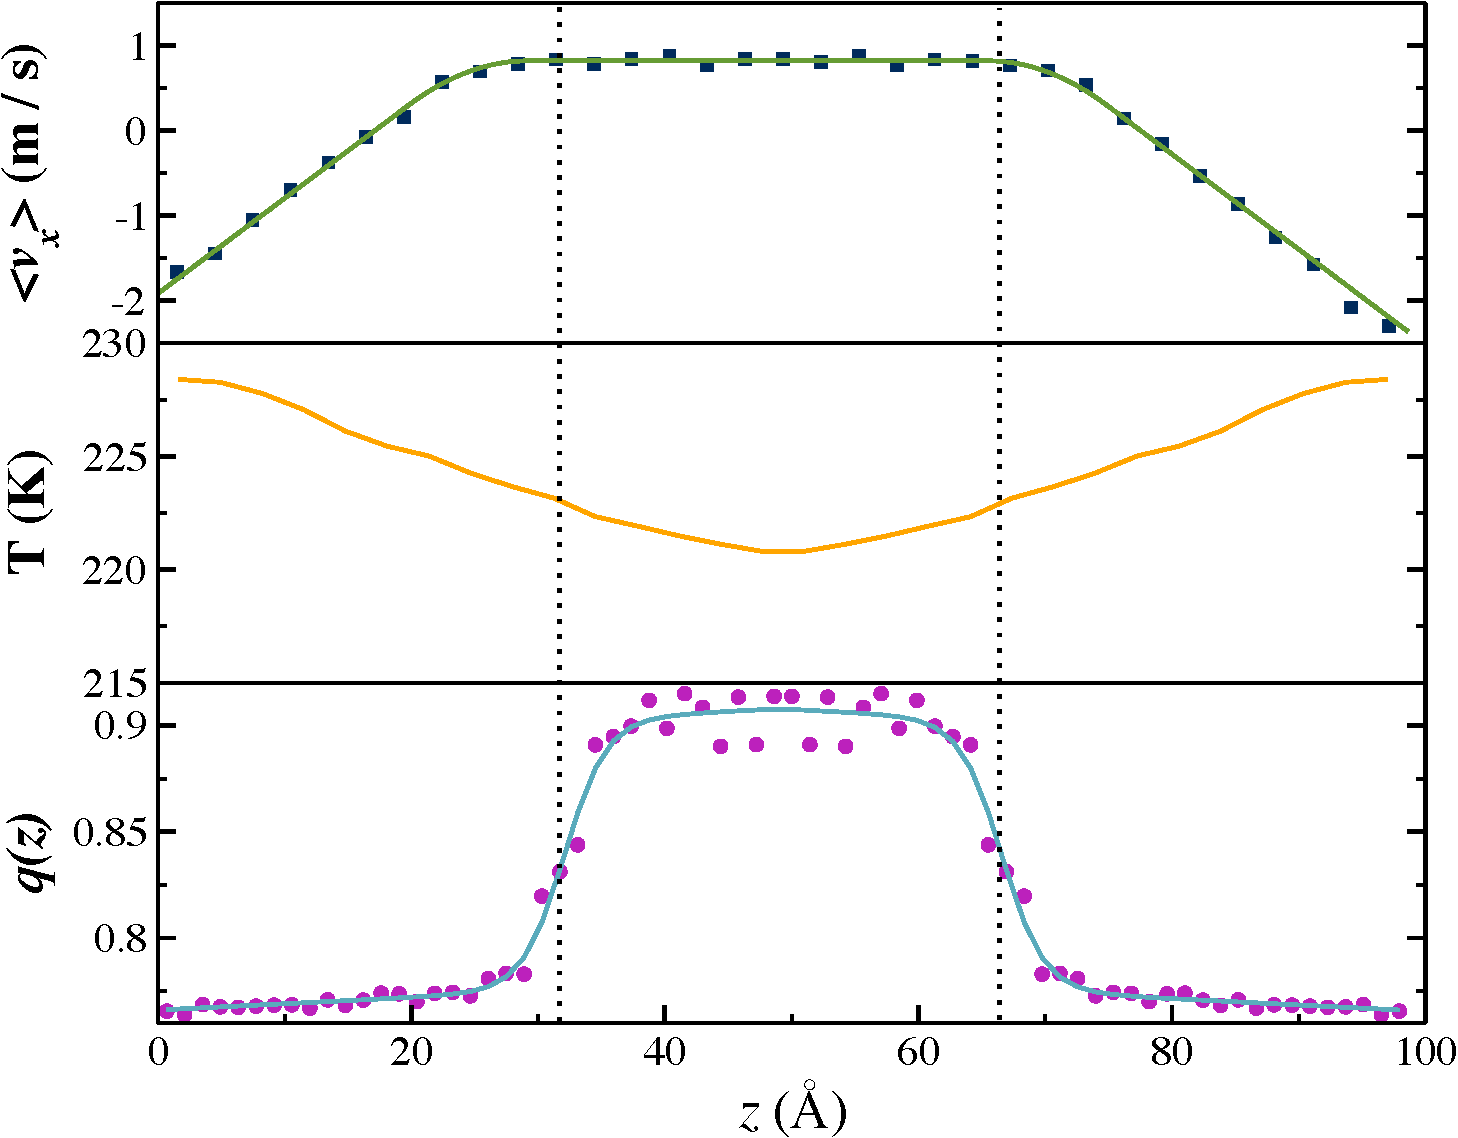
\includegraphics[width=\linewidth]{Figures/Bas_comic_strip}
\caption{\label{fig:bComic} Properties of the basal interface being
  sheared through water at 3.2 ms\textsuperscript{-1}.  Panel
  descriptions are the same as in Fig. \ref{fig:pyrComic}.}
\end{figure}

\begin{figure}
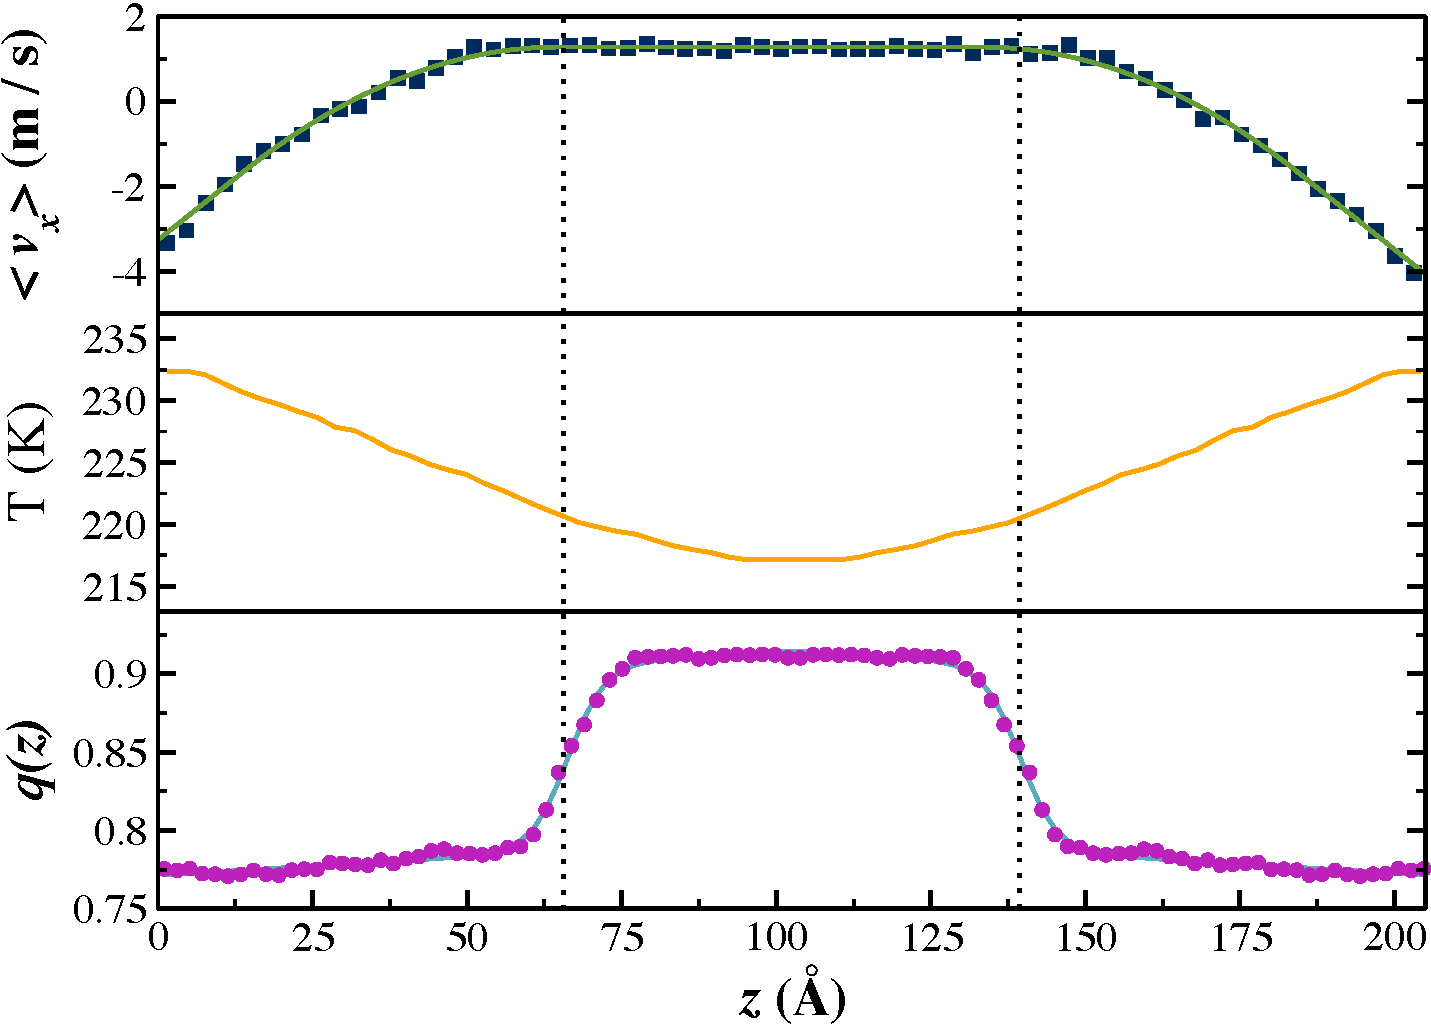
\includegraphics[width=\linewidth]{Figures/Pri_comic_strip}
\caption{\label{fig:pComic} Properties of the prismatic interface
  being sheared through water at 6.0 ms\textsuperscript{-1}.  Panel
  descriptions are the same as in Fig. \ref{fig:pyrComic}.}
\end{figure}
%End figures of z-rnemd profile. 


%Begin z-orientation times                                                         
\begin{figure}
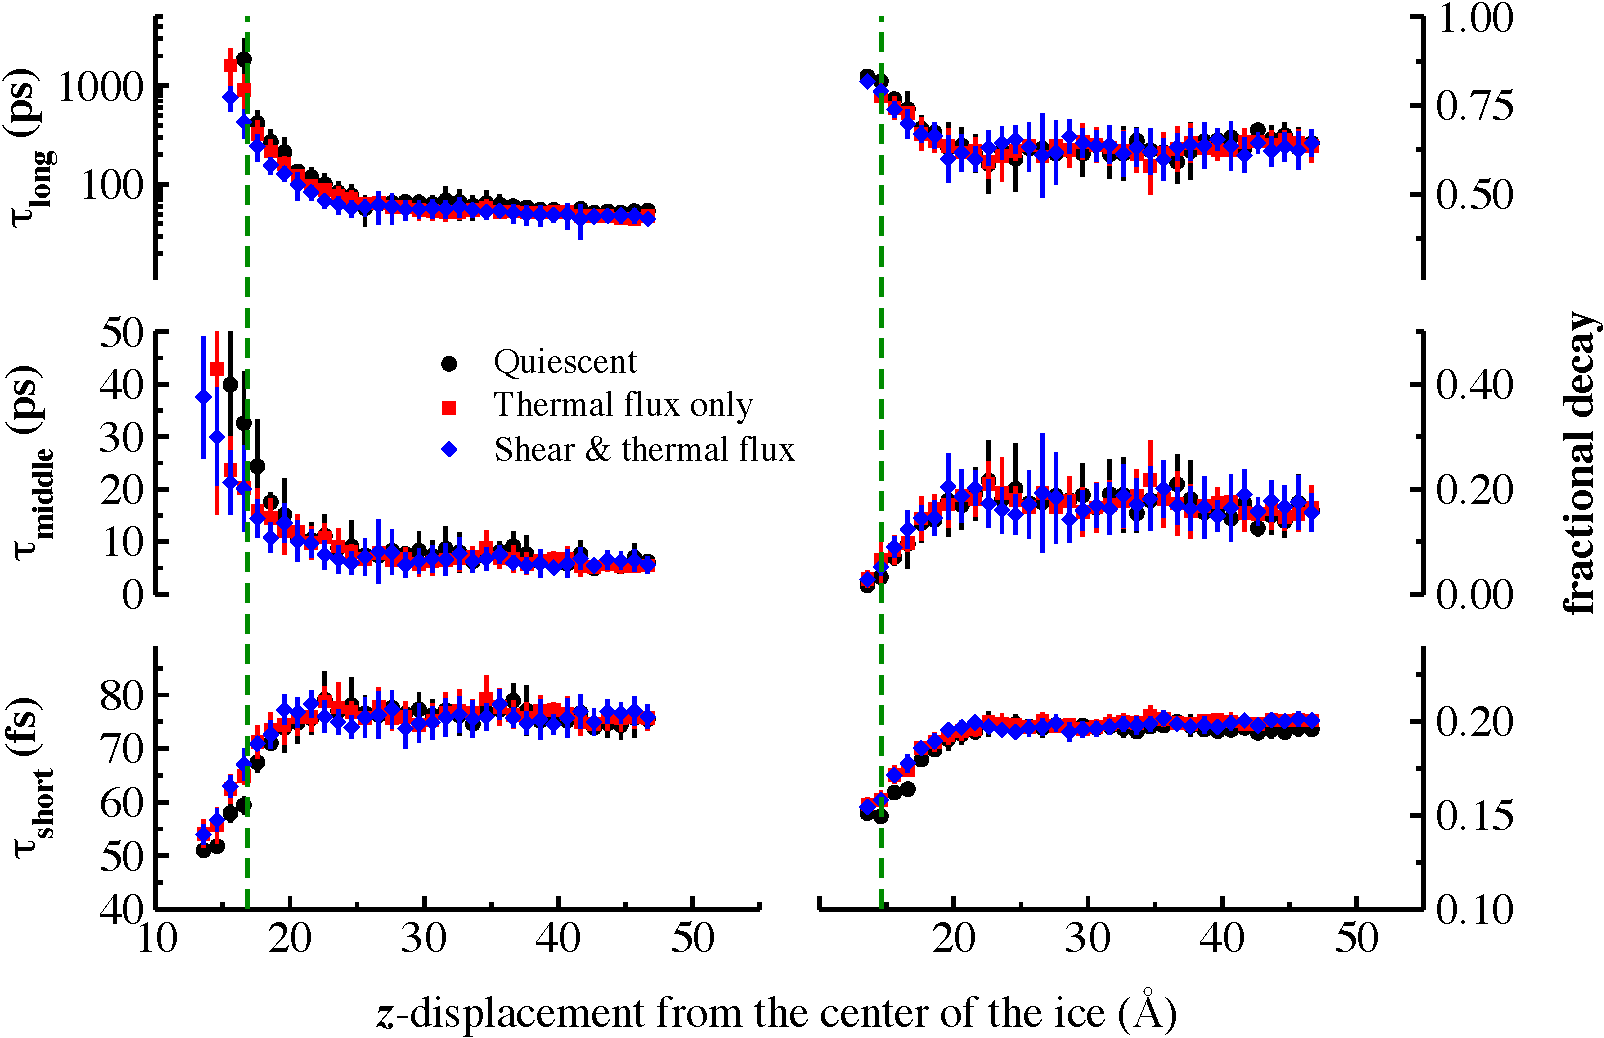
\includegraphics[width=\linewidth]{Figures/Pyr_lcorrz}
\caption{\label{fig:Pyrorient} Decay times (left) for $C_2(z,t)$ at
  the pyramidal interface, and their fractional contributions to the
  overall decay (right) fit using Eq. (8). The local decay constants
  are plotted as a function of distance from the center of the ice
  slab. The vertical dashed line indicates the Gibbs dividing surface
  determined using the local tetrahedral order parameter.  Results are
  shown for a quiescent system with no applied kinetic or momentum
  flux (black), an interface with with an imposed kinetic energy flux
  (red), and a sheared simulation (blue) with both kinetic and
  momentum fluxes.}
\end{figure}

\begin{figure}
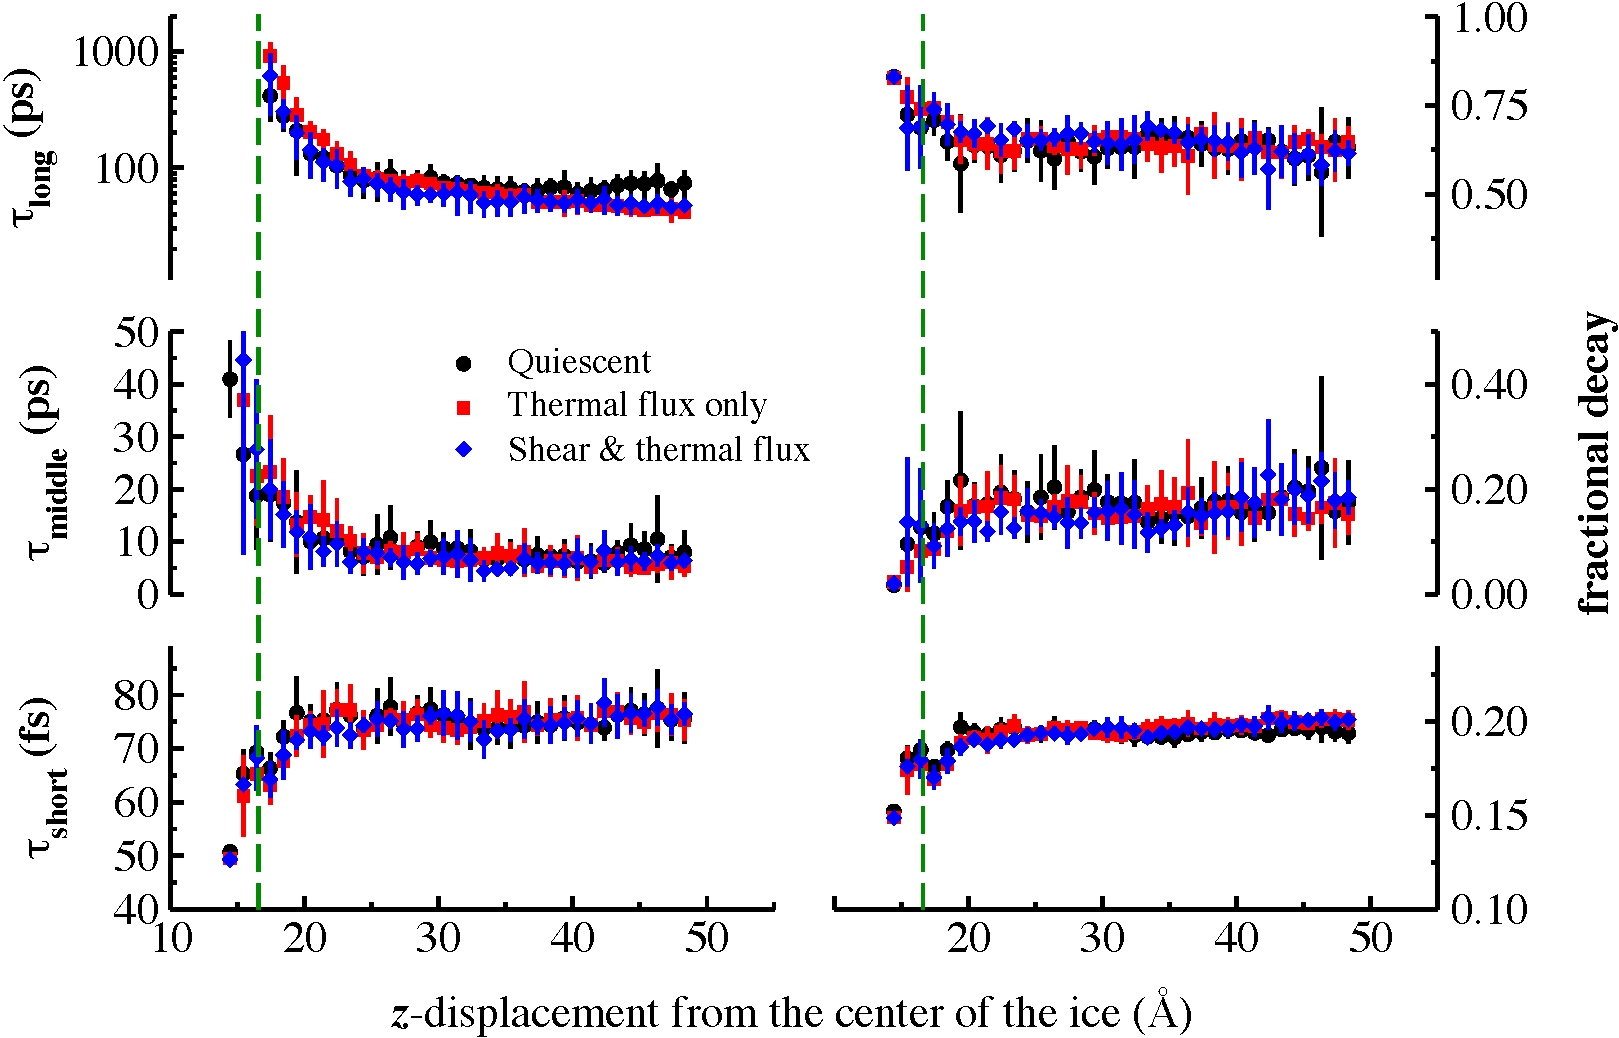
\includegraphics[width=\linewidth]{Figures/Bas_lcorrz}
\caption{\label{fig:Borient} $C_2(z,t)$ time constants for the basal
  interface.  Panel descriptions are the same as in
  Fig. \ref{fig:Pyrorient}. }
\end{figure}

\begin{figure}
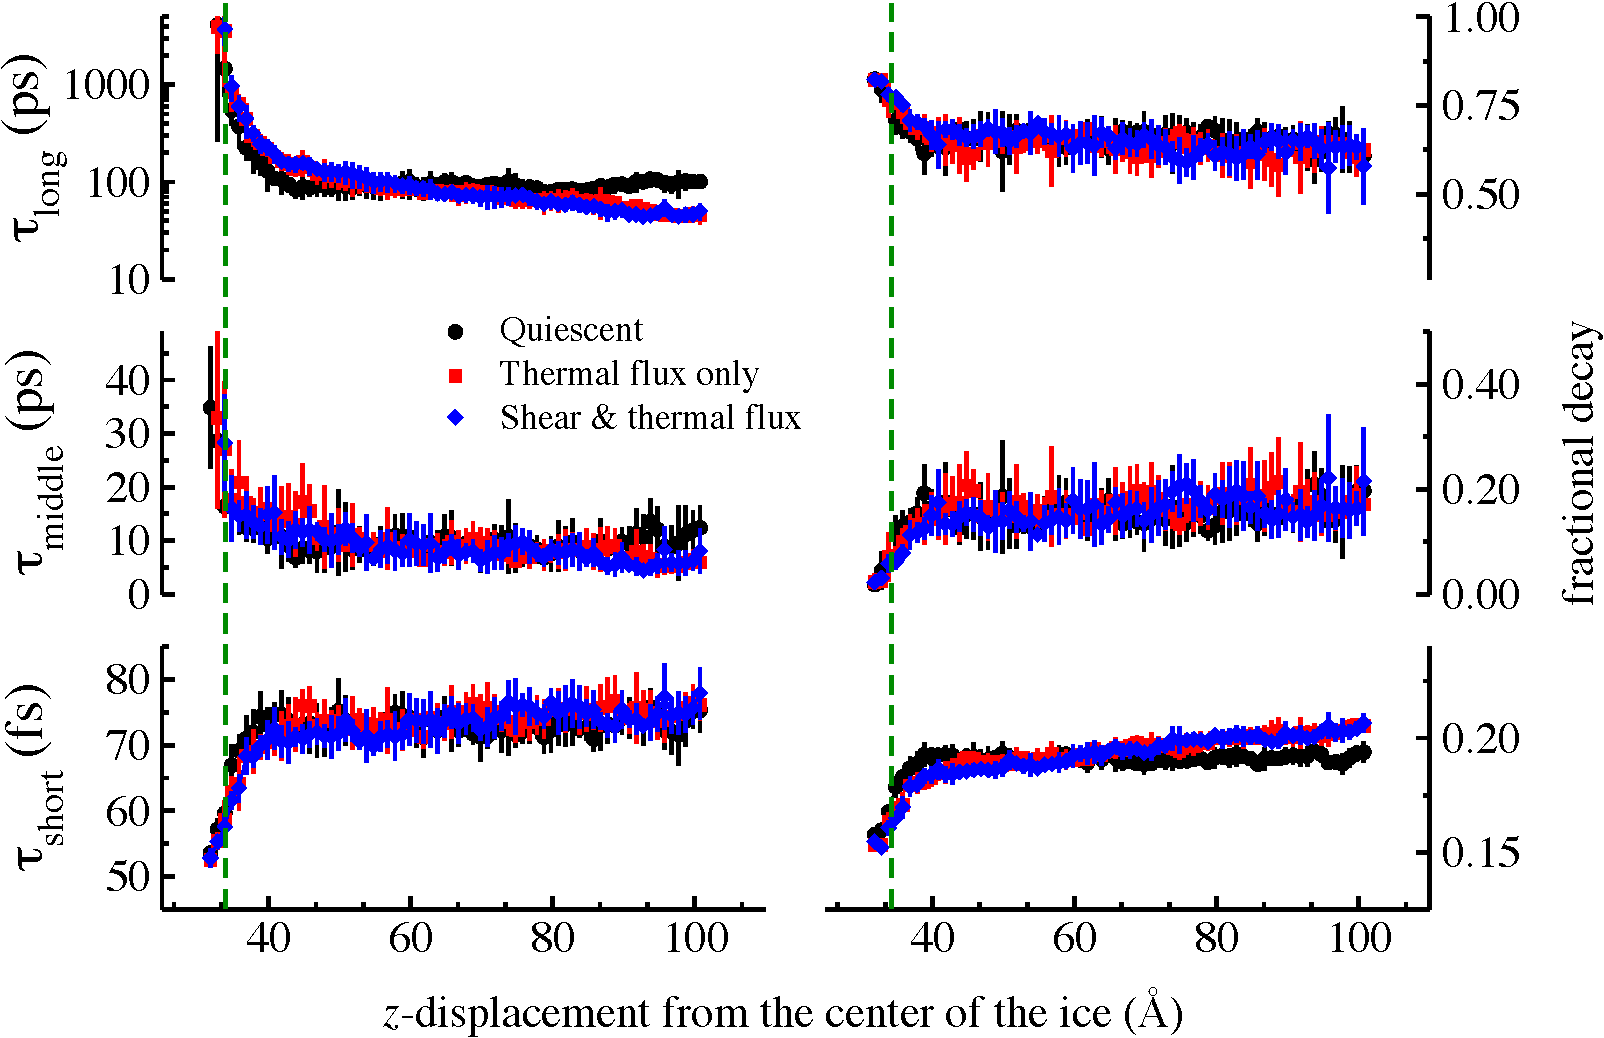
\includegraphics[width=\linewidth]{Figures/Pri_lcorrz}
\caption{\label{fig:Porient} $C_2(z,t)$ time constants for the prismatic
  interface.  Panel descriptions are the same as in
  Fig. \ref{fig:Pyrorient}.}
\end{figure}
%End z-orientation times                                                           
\begin{figure}
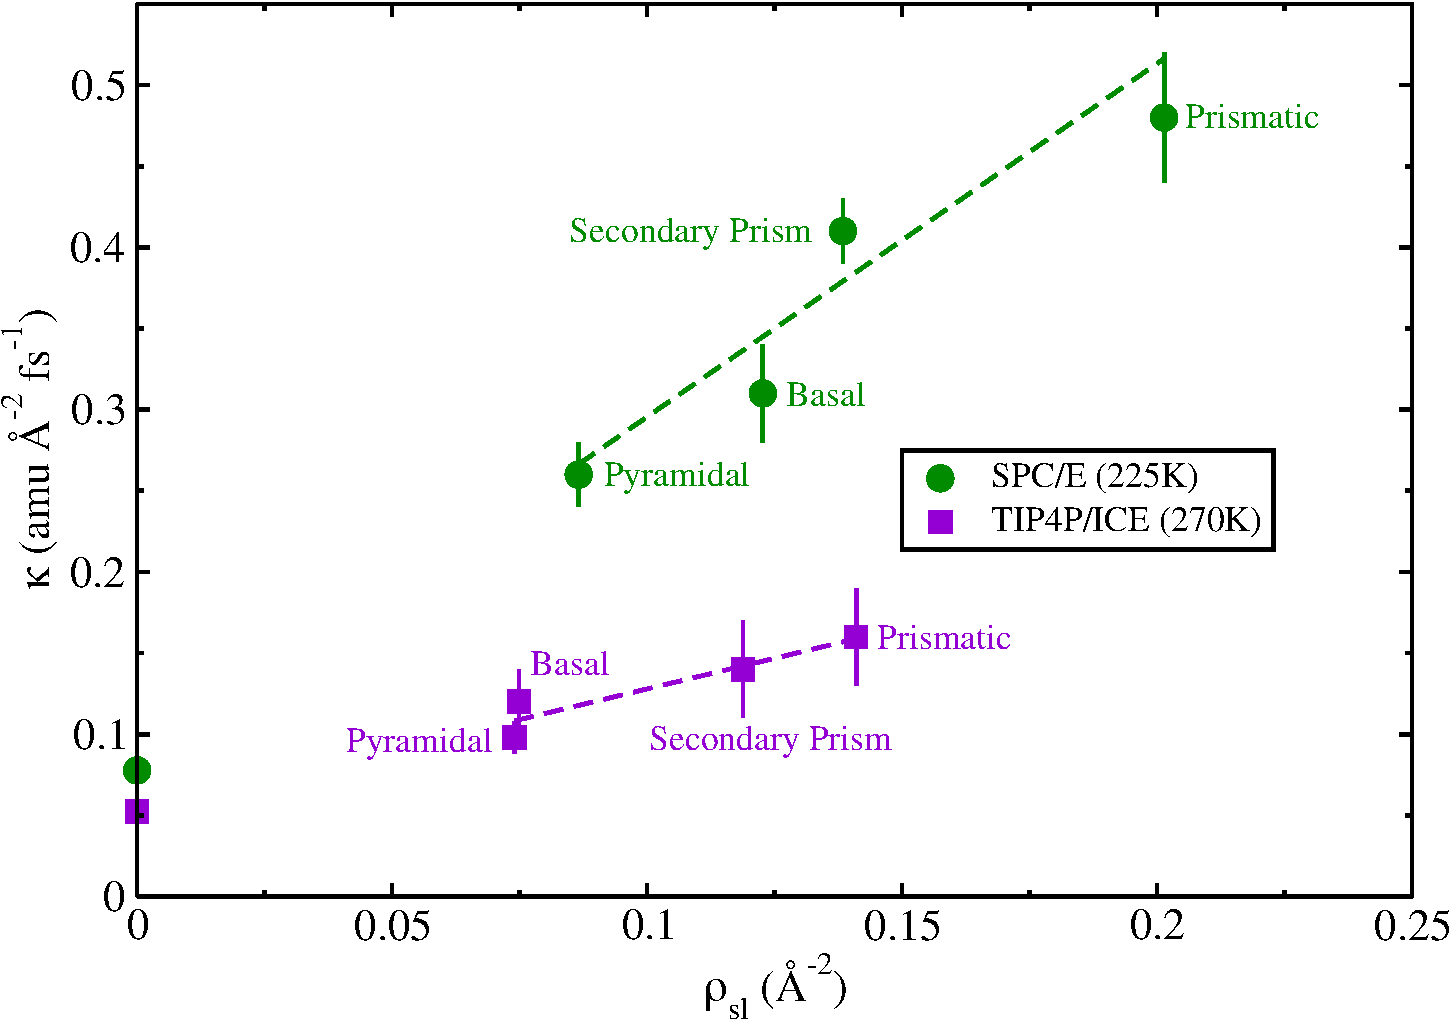
\includegraphics[width=\linewidth]{Figures/hb}
\caption{\label{fig:hbPlot} Solid-liquid friction coefficients by the
  surface density of hydrogen bonds. Linear regression gives a slope
  of 2.1772~(amu~fs\textsuperscript{-1}) and a y-intercept of
  0.0777~(amu~\AA\textsuperscript{-2}~fs\textsuperscript{-1}).} 
\end{figure}                                            


%%%%%%%%%%%%%%%%%%%%%%%%%%%%%%%%%%%%%%%%%%%%%%%%%%%%%%%%%%%%%%%%%%%%%%%%%%%%%%%%%%%
%		CHAPTER 6 -- Shear Viscosity of QLL
%%%%%%%%%%%%%%%%%%%%%%%%%%%%%%%%%%%%%%%%%%%%%%%%%%%%%%%%%%%%%%%%%%%%%%%%%%%%%%%%%%%
\chapter{MEASUREMENTS OF THE VISCOSITY OF THE QUASI-LIQUID LAYER AT THE SURFACE OF ICE-I$_\mathrm{h}$}\label{chap:QLL}

\begin{flushright}
\textit{``All is born of water; all is sustained by water.''} \\
-Johann Wolfgang von Goethe (1817) \\
\end{flushright}

In the hydrodynamic friction regime, there are three distinct
contributions to the overall observed friction; the solid-liquid
friction between the ice and quasi-liquid layer (QLL), the viscous
shearing of the QLL, and the solid-liquid friction between the QLL and
the slider.\cite{Kietzig2009,Kietzig2010} In Chapter
\ref{chap:Friction}, we presented facet-dependent friction
coefficients for the basal, prismatic, 14\degree~pyramidal, and
secondary prism ice-I$_\mathrm{h}$ / water interfaces. In this
chapter, we present an investigation of the temperature dependence of
the shear viscosity of the QLL at the basal and prismatic
ice-I$_\mathrm{h}$ / vapor interfaces.



\section{Computational Methods}

\begin{flushleft}
\textit{Ice Surfaces}
\end{flushleft}

TIP4P/Ice basal and prismatic ice-I$_\mathrm{h}$ primitive crystals
were constructed following the procedure described in Chapter
\ref{chap:Methods}. These primitive cells were then reoriented so that
the desired crystal face was exposed to the $y$ axis, then replicated
in the $x$- and $z$-dimensions to form large sheets. The sheets were
then replicated along the $y$-dimension until the basal crystal was 12
bilayers thick, and the prismatic crystal was replicated to a width of
approximately equal to the basal crystal. Dimensions and number of
molecules in each system are found in Table \ref{tab:qll-method}.


\begin{table}[h]
\centering
\caption{SIZES OF THE VAPOR EXPOSED ICE-I$_\mathrm{h}$ / QUASI-LIQUID LAYER SIMULATIONS\label{tab:qll-method}}
\begin{tabular}{rcccc}
\hline
\hline
 Interface & $N_\mathrm{ice}$ & $L_x$ & $L_y$ & $L_z$ \\
\hline
Basal  $\{0001\}$                           & 46,080 & 185.24 & 44.04 & 186.06 \\
Prismatic  $\{10\bar{1}0\}$            & 55,000 & 192.47 & 49.14 & 181.61\\
\hline
\hline
\end{tabular}
\begin{flushleft}
Box dimensions are given in \AA.
\end{flushleft}
\end{table}


The $y$-dimension of the simulation box was then set to 300~\AA~ to
allow for a surface premelt to form, and replicas of each system were
equilibrated to four temperatures, 255, 260, 265, and 270~K at
1~atm. The resulting systems exposed two interfaces, one toward
positive $y$ and the other towards negative $y$. Equilibration was
conducted under a constant surface tension and temperature integrator,
allowing the $x$- and $z$-dimensions of the simulation cell to relax
and alleviate any crystal strain. Following this, the systems were
equilibrated under a constant volume and temperature integrator (NVT),
and lastly under a constant volume and energy integrator (NVE). During
these simulations, the width of the crystal (in the $y$-dimension) was
monitored to ensure no appreciable crystal melt or large scale
restructuring occurred. Once equilibration was complete, a 100 ps
production simulation was performed for each system, where the
positions and velocities were recored every 0.1 ps.



% In Chapter \ref{chap:Str}, we found the
% tetrahedrality at the Gibbs dividing surface for ice-I$_\mathrm{h}$ /
% water interfaces to be $q^{Gibbs} \sim$0.84. Here, we have used
% $q^{Gibbs}$ as the cutoff value between the QLL and the ice. All
% molecules with $q < q^{Gibbs}$ are denoted as QLL molecules, while
% those with $q > q^{Gibbs}$ are denoted to be ice. This cutoff
% coincides with a minimum in the tangential density profiles, as seen
% in the top and bottom panels of Figure \ref{fig:qll-rhoq}.


\begin{flushleft}
\textit{Supercooled Liquids}
\end{flushleft}
As a comparison to the structure and dynamics of the quasi-liquid
layer of ice, we have performed simulations of supercooled bulk liquid using the
TIP4P/Ice potential. A cubic box of 4,000 water molecules was
constructed and replicas were equilibrated to 255~K, 260~K, 265~K, and
270~K at 1 atm. System sizes and corresponding densities are presented in Table
\ref{tab:qll-liquid}. Once the liquid boxes were equilibrated, four
successive one nanosecond simulations were performed under an NVE
integrator. During these simulations, the positions and velocities
were stored every 100 fs.

\begin{table}[h] \centering \caption{SYSTEM SIZES AND DENSITIES OF THE SUPERCOOLED BULK LIQUID\label{tab:qll-liquid}}
\begin{tabular}{cccc}
\hline
\hline
 Temperature & $N_\mathrm{molecules}$ & $L_x, L_y, L_z$ & $\rho$\\
\hline
270 & 4,000 & 50.1512 & 0.9487 \\
265 & 4,000 & 50.1305 & 0.9499 \\
260 & 4,000 & 50.1821 & 0.9469 \\
255 & 4,000 & 50.2494 & 0.9437 \\
\hline
\hline
\end{tabular}
\begin{flushleft}
Temperatures, box dimensions, and densities are given in K, \AA~, and
$\mathrm{g}~\mathrm{cm}^{-3}$, respectively.
\end{flushleft}
\end{table}



\section{Simulations of Supercooled Liquid}
Henson \textit{et al.} predicted that the QLL should behave as a
supercooled bulk liquid.\cite{Henson2005} Studying supercooled liquids
experimentally, however, can be quite challenging. Besides possibly
skewing results, contaminants can also act as nucleation sites for
crystal growth. Due to this, much of our insight on supercooled liquid
water comes from molecular simulations. Crystal growth is an extremely
slow process on the computational timescale, allowing for
investigations of bulk liquid in this temperature regime. 

\subsection{Structural Measures of Supercooled Water}

\begin{flushleft}
\textit{Pair Distribution Function}
\end{flushleft}

The pair distribution function, $\mathrm{g}(r)$, provides information
regarding the spatial distribution of molecules. Calculation of this
function was achieved by compiling the average number of molecules
found to be a distance $r$ to ($r + \delta r$) apart. The
pair density $\rho (r)$ of each of these small shells is normalized by
the system's bulk density and the shell volume.
\begin{equation}\label{eq:gofr}
\mathrm{g}(r) = \rho(r) / \rho^{bulk}
\end{equation}
Equation \eqref{eq:gofr} is a general relation which can be used for
pairs of atoms, molecules, or even assemblies. Here, we have have
computed $\mathrm{g}(r)$ for pairs of water molecules, as
seen in the lower panel of Figure \ref{fig:gofrQ}

\begin{figure*}
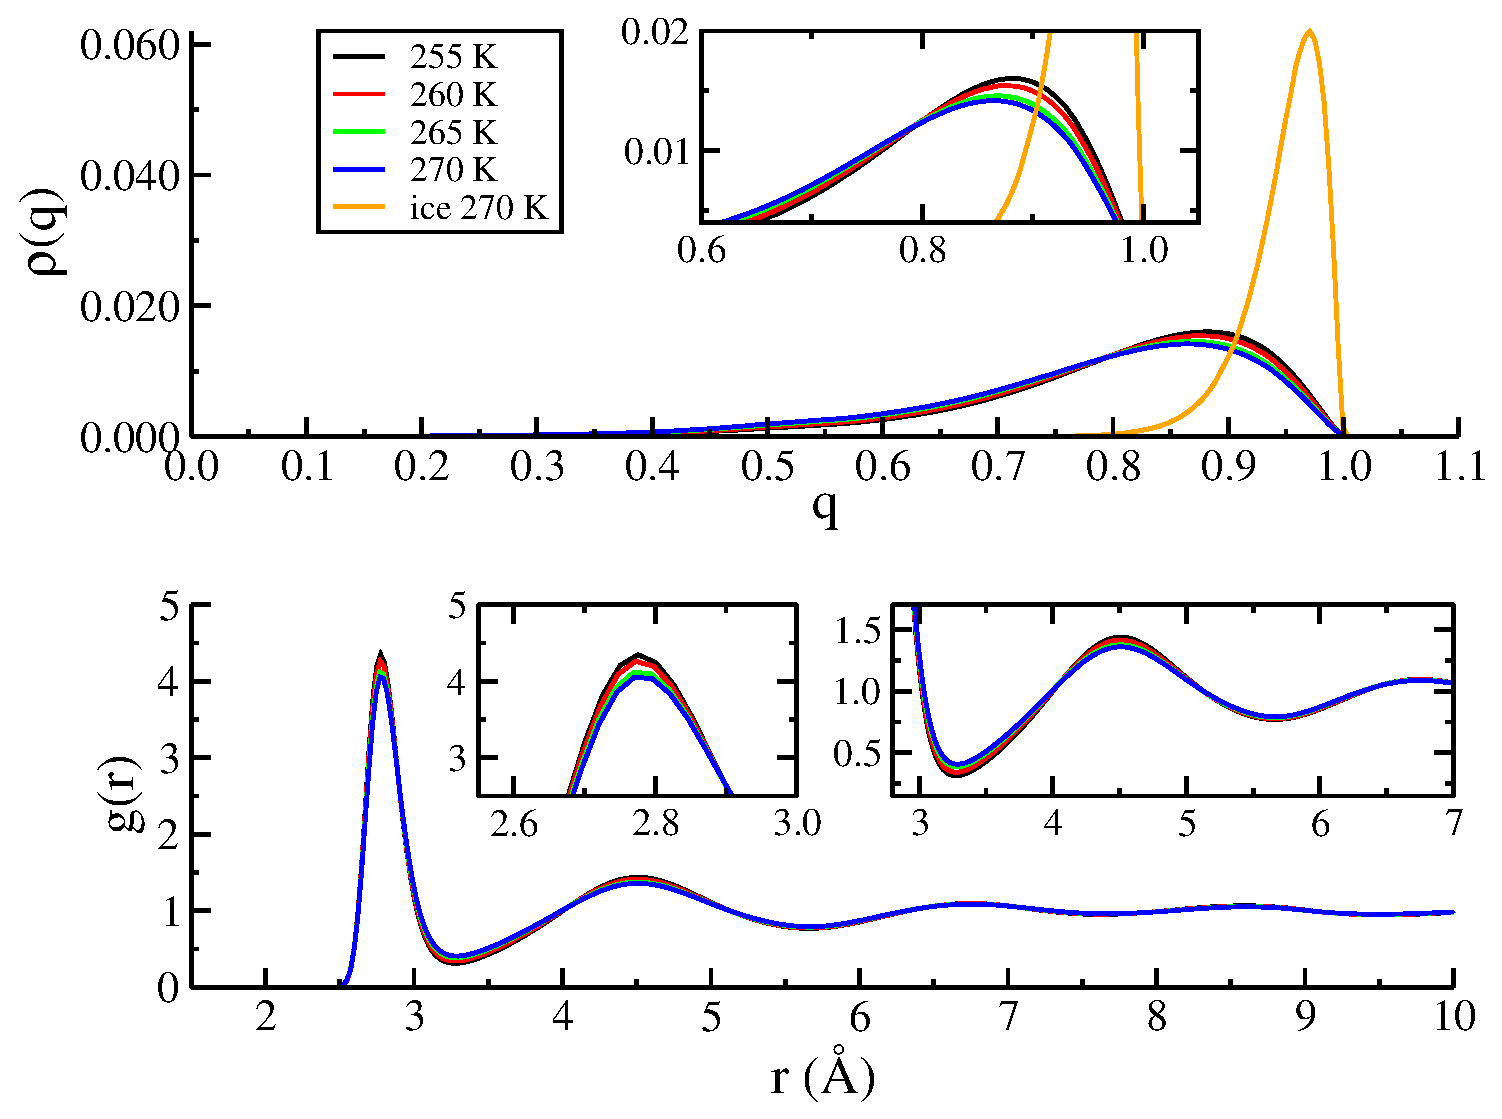
\includegraphics[width=\linewidth]{Figures/bulk_GofrQdens}
\caption{\label{fig:gofrQ} Pair distribution function
  $\mathrm{g}(r)$ and probability density distributions of
  the local tetrahedral order parameter $\rho (\mathrm{q})$ for
  supercooled liquid water.}
\end{figure*}  

We observe no population of pairs of water molecules at small values
of $r$. This is due to the size of a water molecule, modeled
by the repulsive portion of the Lennard-Jones potential. The large
peak at $r~\sim$ 2.8 corresponds to the first solvation
shell around the water molecules. The dip immediately following this
peak indicates a region of low population, followed by a second
smaller peak. This second peak captures the second solvation shell of
water, which is more diffuse than the first. At larger values of
$r$ the function approaches unity, indicating at large
separations the liquid ordering reflects that of the bulk. 

The two insets are closer views of the first and second solvation
shells. We see for colder temperature, the liquid becomes slightly
more ordered, apparent from the increase in the first and second
solvation shells, as well as the decrease in the population between
the two shells. In order to quantify this ordering, it is
common to integrate $\mathrm{g}(r)$ to determine the
coordination number $n_c$.
\begin{equation}\label{eq:nofr}
n_c = 4 \pi \rho^{bulk} \int_0^{r_m} g(r)r^2dr
\end{equation}


\begin{table}[h] \centering \caption{LOCATION AND INTEGRATION OF THE
    RADIAL DISTRIBUTION FUNCTION AT THE FIRST SOLVATION SHELLS AND
    FRACTIONAL DENSITIES OF NUMBER OF HYDROGEN BONDS FORMED FOR
    SUPERCOOLED LIQUID\label{tab:gofr}}
\begin{tabular}{ccccccc}
  \hline
  \hline
  Temperature & $r_m$ & $n_c$ & $\rho_\mathrm{HB}(2)$ & $\rho_\mathrm{HB}(3)$ & $\rho_\mathrm{HB}(4)$ & $\rho_\mathrm{HB}(5)$ \\
  \hline
  270 & 3.297 &4.1523(3) & 0.01645(3) & 0.1531(9) & 0.7771(3) & 0.05231(1)\\
  265 & 3.271 & 4.1056(7) & 0.01447(57) & 0.1432(4) & 0.7907(8) & 0.0507(2)\\
  260 & 3.299 & 4.060(1) & 0.01126(6) & 0.1246(3) & 0.8172(4) & 0.0462(2)\\
  255 & 3.253 & 4.06024(6)  & 0.0096(1) & 0.1138(4) & 0.8330(9) &
                                                                  0.0431(4) \\
  \hline
  \hline
\end{tabular}
\begin{flushleft}
Temperatures are reported in K. Uncertainties are given in parentheses.
\end{flushleft}
\end{table}

We find that the location of the minimum following the first peak
$r_m$ in $\mathrm{g}(r)$ is at slightly larger values of $r$ with
increasing temperature. Taking this as the limit of integration, the
coordination number for the first solvation shell, $n_c$ was computed
(see Table \ref{tab:gofr}). Similarly, $n_c$ is observed to increase with
increasing temperature. Since the supercooled liquid's density
increases with increasing temperature, we should expect a larger
coordination number with increasing temperature in this regime.

\begin{flushleft}
\textit{Density of Hydrogen Bonds}
\end{flushleft}

It is well known that water forms four hydrogen bonds in hexagonal
ice. In the liquid, water often adapts configurations which results in
a smaller number of hydrogen bonds. As an additional probe of the
supercooled liquid structure, we have computed the average fractional
populations of hydrogen bond participation ($\rho_\mathrm{HB}$) at
each of the four temperatures. To do so, we have used the hydrogen
bonding criteria of Luzar and Chandler, which requires the
oxygen-oxygen distance to be less than 3.4~\AA~, and the
oxygen-hydrogen-oxygen angle to be less than
30\degree.\cite{Luzar1996} This criteria has been shown to give good
agreement with energetic definitions of hydrogen bonds, as the
geometric and energetic definitions are intimately coupled. The
resulting fractional participation statistics can be found in Table
\ref{tab:gofr}.


% \begin{table}[h] \centering \caption{FRACTIONAL DENSITIES OF NUMBER OF
%     HYDROGEN BONDS FORMED FOR SUPERCOOLED LIQUID\label{tab:bulk_HB}}
% \begin{tabular}{ccccc}
% \hline
% \hline
%  Temperature & $\rho_\mathrm{HB}(2)$ & $\rho_\mathrm{HB}(3)$ & $\rho_\mathrm{HB}(4)$ & $\rho_\mathrm{HB}(5)$  \\
% \hline
% 270 & 0.01645(3) & 0.1531(9) & 0.7771(3) & 0.05231(1)\\
% 265 & 0.01447(57) & 0.1432(4) & 0.7907(8) & 0.0507(2)\\
% 260 & 0.01126(6) & 0.1246(3) & 0.8172(4) & 0.0462(2)  \\
% 255 & 0.0096(1) & 0.1138(4) & 0.8330(9) & 0.0431(4) \\
% \hline
% \hline
% \end{tabular}
% \begin{flushleft}
% Temperatures are reported in K. Uncertainties are given in parentheses.
% \end{flushleft}
% \end{table}

Here, we observe a clear temperature dependence on the fractional
populations of of hydrogen bonds participation formed in the
liquid. At colder temperatures, we find a larger fraction of the
population form four hydrogen bonds. However, at warmer temperatures,
the reduction in population of four hydrogen bonded molecules results
in larger densities of molecules with two and three hydrogen bonds.



\begin{flushleft}
\textit{Density of Tetrahedral Ordering}
\end{flushleft}

While the pair distribution function provides information about
the spatial separation of molecules, it fails to discriminate any
orientational ordering which may be present in the liquid. In order to
query this orientational ordering, the density of local tetrahedral
order parameters, $\rho (q)$, observed during the simulation was
computed (see Figure \ref{fig:gofrQ}). This was accomplished by
computing $q$ for every molecule at each configuration, and determining
the fractional number of molecules which adopted this configuration.

In Figure \ref{fig:gofrQ}, we see a noticeable trend in $\rho (q)$
with increasing temperature. The $q$-value of the peak in the density
distribution decreases with increasing temperature. This indicates
that for warmer simulation temperatures, the tetrahedral ordering of
the liquid decreases. All four liquid simulations give a much broader
distribution than observed for a commensurate ice-I$_\mathrm{h}$
crystal at 270 K.





\subsection{Dynamic Measures of Supercooled Water}
At colder temperatures, we should expect the dynamics of water to be
slower simply due to lower kinetic energy. However, at colder
temperatures, water molecules may adapt structures which further hinder
dynamics. Since the density of tetrahedrality indicated an
orientational ordering in the liquid which was sensitive to
temperature, we may expect to observe temperature dependent dynamics
as well. Here, we have investigated both \textit{translational} and
\textit{orientational} measures of dynamics.

\begin{flushleft}
\textit{Diffusion in the Supercooled Liquid}
\end{flushleft}

Diffusion coefficients for water molecules in ice are approximately
zero, as the small amount of diffusion that is observed is highly
dependent on the presence of lattice defects. In contrast, diffusion
of water molecules in supercooled liquid is observed well below the
freezing point.\cite{Debenedetti2003} Pruppacher has measured the
diffusion of supercooled liquid down to -25\degree~C using a tritium
tracer.\cite{Pruppacher1972} In order to compare with the diffusion of
the quasi-liquid layers, we have computed three dimensional diffusion
coefficients for each of the bulk liquid simulations. Mean squared
displacements were computed for each of the supercooled liquid systems
(see lower panel of Figure \ref{fig:bulkD}), and the non-spatially
resolved version of Equation \eqref{eq:yDiff} was used to compute
average diffusion coefficients (see upper panel of the same figure).

\begin{figure*}
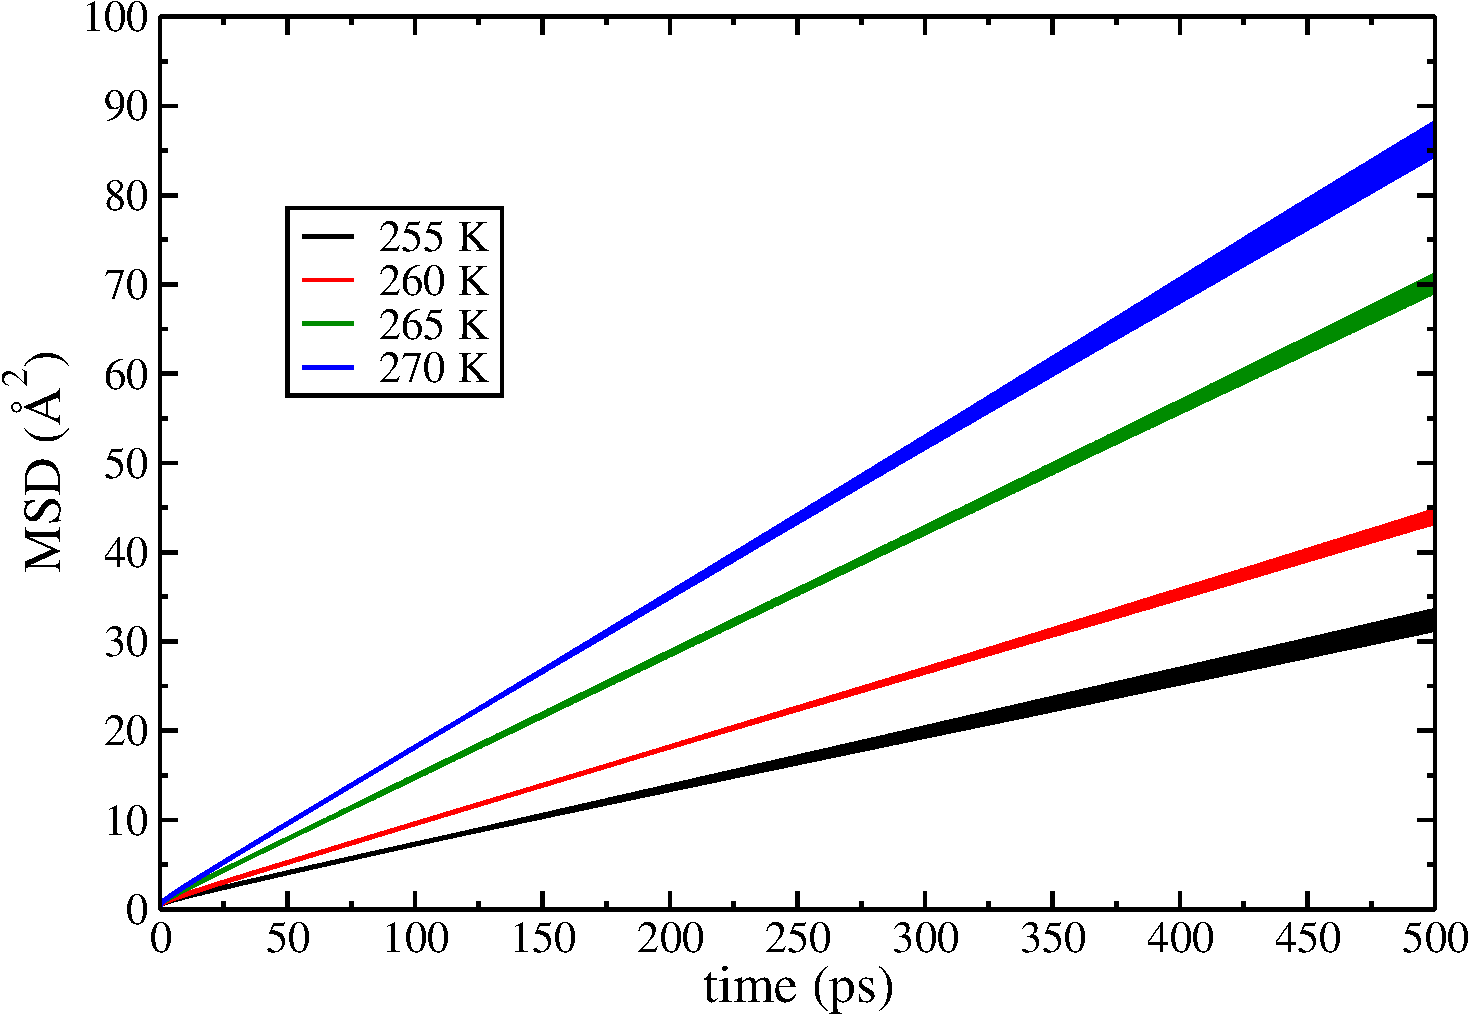
\includegraphics[width=\linewidth]{Figures/bulkD}
\caption{\label{fig:bulkD} Lower panel: mean squared displacements
  (MSD) for supercooled liquid water. Upper panel: three dimensional
  diffusion constants computed from the MSD data in the lower panel. }
\end{figure*}    
 
We estimate diffusion coefficients of
$\mathrm{D}~\sim~ 1.0 \times 10^{-5}
(\mathrm{\AA}^{2}~\mathrm{fs}^{-1})$ to
$\mathrm{D}~\sim~ 3.0 \times 10^{-5}
(\mathrm{\AA}^{2}~\mathrm{fs}^{-1})$ for the range of temperatures
investigated. % The data are fit well with a linear regression giving a
% rate of change between the data of
% $0.1254 \times 10^{-5}~\mathrm{D}/\mathrm{K}$.


\begin{flushleft}
\textit{Orientational Decorrelation}
\end{flushleft}

Orientational time correlation functions provide information on the
decorrelation of molecular environments. As we observed in Chapter
\ref{chap:Dyn}, decorrelation times in ice go asymptotically to
infinity, while in liquid, values in the ps to ns range are more
common. In Chapter \ref{chap:Dyn} we computed a spatially resolved
version of the orientational time correlation function to probe how
the dynamics of molecules changed approaching the ice-I$_\mathrm{h}$ /
water interface. Here, all of the water molecules should behave
identically over a long time average as there are no interfaces present.
\begin{equation}\label{C(t)}
  C_{2}(t)=\langle P_{2}(\mathbf{u}_i(0)\cdot \mathbf{u}_i(t))\rangle,
\end{equation}
Again, $P_2$ is the second-order Legendre polynomial, 
$\mathbf{u}_i$ is the molecular unit vector that bisects the HOH angle
of molecule $i$, and the angle brackets denotes an average over all
molecules and time origins. Computed C$_2$(t) is shown in the lower
panel of Figure \ref{fig:jump_lcorr}.

There are three modes available for decorrelation of $C_2(t)$. Fitting
computed $C_2(t)$ by a triexponential decay which captures the
characteristic times for these modes can provide insight on the
temperature dependence of the reorientation of supercooled liquid
water. The three time constants: $\tau_\mathrm{short}$, measuring the
librational motion of the water molecules, $\tau_\mathrm{middle}$,
measuring the timescale for the large angle jumps during the breaking
and making of hydrogen bonds, and $\tau_\mathrm{long}$, corresponding
to the translational motion of the water molecules, can be obtained
by\cite{Louden2013a}
\begin{equation}
  C_{2}(t) = a~e^{-t/\tau_\mathrm{short}} + b~e^{-t/\tau_\mathrm{middle}} + 
  (1-a-b)~e^{-t/\tau_\mathrm{long}}.
\label{eq:c2}
\end{equation}
Here, the coefficients $a$, $b$, and $(1-a-b)$ give the fractional
amount of the total decay due to that particular mode. Averages of the
decay constants and their coefficients are reported in Table
\ref{tab:supOrient}.


\begin{table}[h] \centering \caption{OREINTATIONAL DECAY TIMES AND
    THEIR FRACTIONAL CONTRIBUTIONS FOR SUPERCOOLED WATER\label{tab:supOrient}}
\begin{tabular}{ccccccc}
\hline
\hline
 Temperature & $a$ & $\tau_\mathrm{short}$& $b$ &
                                                  $\tau_\mathrm{middle}$
  & $(1-a-b)$ & $\tau_\mathrm{long}$\\
\hline
270 &0.2235(3) &85.1(3) & 0.165(2) & 3.75(5) & 0.611(2) & 26.1(2)\\
265 &0.2191(4) &86.0(2) & 0.174(4) & 4.8(1) & 0.607(5) & 34(1)\\
260 &0.2117(3) &87.5(2) & 0.190(6) & 7.7(3) & 0.599(6) & 59(1)\\
255 &0.2060(5) &87.2(4) & 0.183(7) & 9.6(5) & 0.611(8) & 81(2)\\
\hline
\hline
\end{tabular}
\begin{flushleft}
Temperatures are given in K, $\tau_{short}$ is reported in fs, while $\tau_{middle}$ and
$\tau_{long}$ are given in ps. Uncertainties are given in parentheses.
\end{flushleft}
\end{table}

We observe a very clear temperature dependence in
$\tau_\mathrm{short}$, $\tau_\mathrm{middle}$, and
$\tau_\mathrm{long}$; for increasing temperatures, the decay time
decreases. We find the fast librational motion decay time to be
between 85 fs and 87 fs, while the slower hydrogen bond dynamics and
frame reorientation characteristic times of 4-10 ps, and 26-80 ps
respectively.  The fractional contribution of the short time
contribution increases with increasing temperature, while the
contributions due to hydrogen bond making and breaking events
contributes less with increasing temperature. The contribution of the slow frame
reorientation appears to be invariant to temperature, with 60$\%$
of the decay given by frame reorientation.


\begin{figure*}
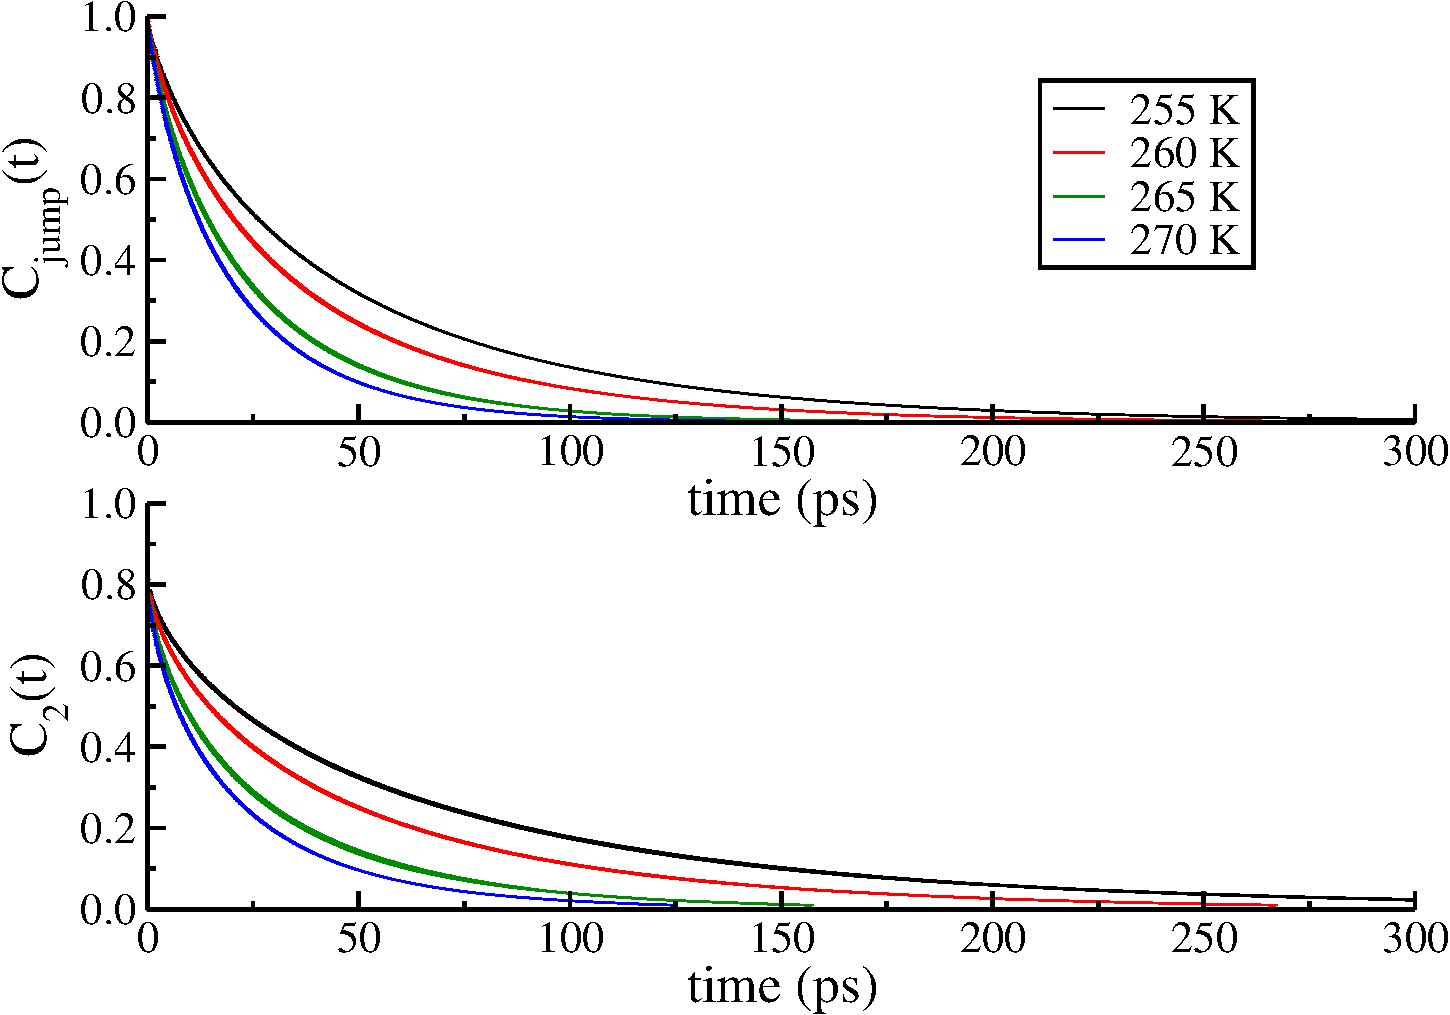
\includegraphics[width=\linewidth]{Figures/jump_lcorr}
\caption{\label{fig:jump_lcorr} The orientational time correlation
  function C$_2$(t) (lower panel) and the hydrogen bond jump
  correlation function C$_\mathrm{jump}$(t) (upper panel) for
  supercooled liquid water. }
\end{figure*}                


\begin{flushleft}
\textit{Hydrogen Bond Jump Times}
\end{flushleft}
The hydrogen bond jump time measures the decorrelation of a hydrogen
bond between two water molecules, $a$ and $b$. 
\begin{equation}\label{jump}
C_\mathrm{jump}(t) = 1 - \langle n_a(0) n_b(t) \rangle
\end{equation}
$n_a(0)$ is set to 1 if hydrogen $i$ is bound to water molecule $b$ at
time ($t=0$), and set to zero otherwise. A spatially resolved version
of this correlation function was described in Chapter \ref{chap:Dyn},
while here we are interested in the temperature dependence of the
hydrogen bond jump times. Again absorbing boundary conditions were
applied, \textit{i.e.} any back jumps were considered new hydrogen
bond formation events.

The hydrogen bond jump correlation function was computed for each of
the bulk liquid simulations, and the resulting $C_\mathrm{jump}(t)$
are plotted in the upper panel of Figure \ref{fig:jump_lcorr}. These
were found to be well fit by a single exponential decay, with a decay
constant describing the jump time for breaking and making hydrogen
bonds. From these characteristic decay times the jump rate can be
determined $k_\mathrm{jump} = \tau_\mathrm{jump}^{-1}$. These jump
rates are presented in Table \ref{tab:bulkJump}. We observe a clear
temperature dependence in the jump rates, at colder temperatures the
jump rates are smaller, around $k_\mathrm{jump} = 0.016$ (ps$^{-1}$),
and at warmer temperatures $k_\mathrm{jump} = 0.04$ (ps$^{-1}$).

\begin{table}[h] \centering \caption{HYDROGEN BOND JUMP RATES FOR THE
    SUPERCOOLED BULK LIQUID\label{tab:bulkJump}}
\begin{tabular}{cc}
\hline
\hline
 Temperature & $k_\mathrm{jump}$ \\
\hline
270 & 0.0402(7) \\
265 & 0.0328(7) \\
260 & 0.0207(3)  \\
255 & 0.0160(5) \\
\hline
\hline
\end{tabular}
\begin{flushleft}
  Temperatures are given in K, and jump rates are presented in
  ~ps$^{-1}$. Uncertainties are given in parentheses.
\end{flushleft}
\end{table}


\section{Characterization of the Quasi-Liquid Layer}
Formation of a quasi-liquid layer on the basal and prismatic surfaces
of ice-I$_\mathrm{h}$ was observed at all temperatures
investigated. Characterizing this surface premelt can be achieved by a
variety of order parameters. Here, we have chosen two structural
parameters, the local density and the local tetrahedral order
parameter described in Chapter \ref{chap:Str}. To compute profiles of
these measures, each of the systems investigated were divided into
small bins ($\delta y$) and an average of the order parameter was
computed for that bin. The resulting profiles for the basal and
prismatic systems at each temperature are presented in Figures
\ref{fig:basal_rhoq} and \ref{fig:prism_rhoq}.

\begin{figure*}
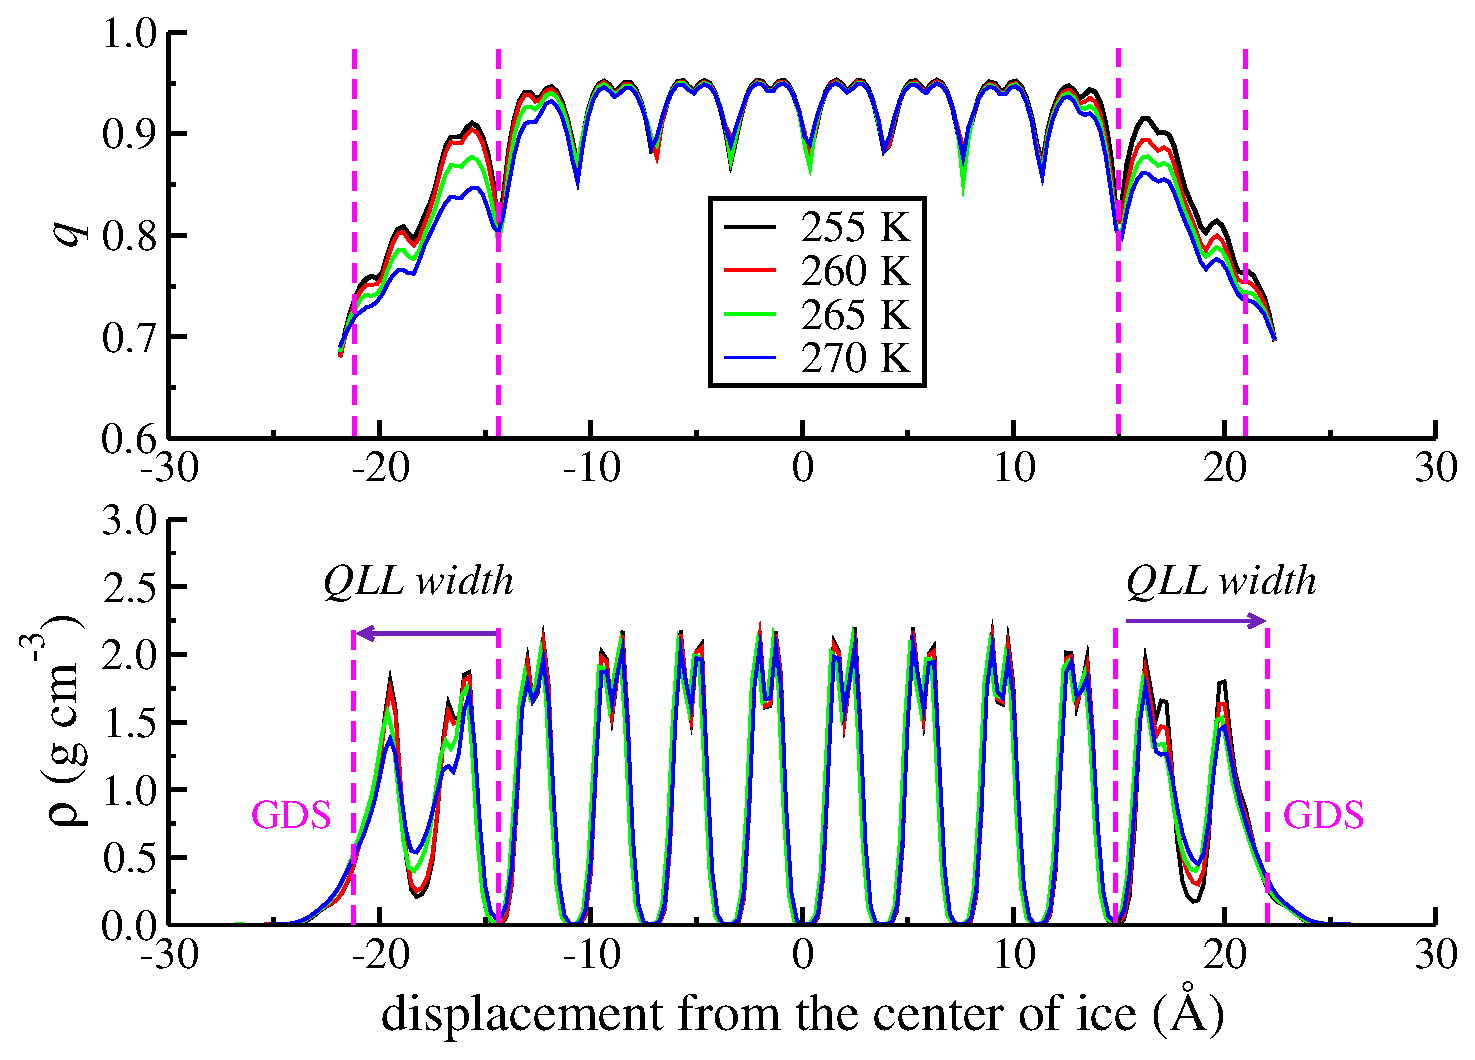
\includegraphics[width=\linewidth]{Figures/basal_qdens}
\caption{\label{fig:basal_rhoq} The spatially resolved average density
  (lower) and local tetrahedral order parameter (upper) of the
  exposed basal ice-I$_\mathrm{h}$ crystal. Quasi-liquid layer (QLL)
  formation is observed in the outermost water bilayers. The Gibbs
  dividing surface of the QLL / vapor interface is indicated by
  vertical magenta lines. }
\end{figure*}                


\begin{figure*}
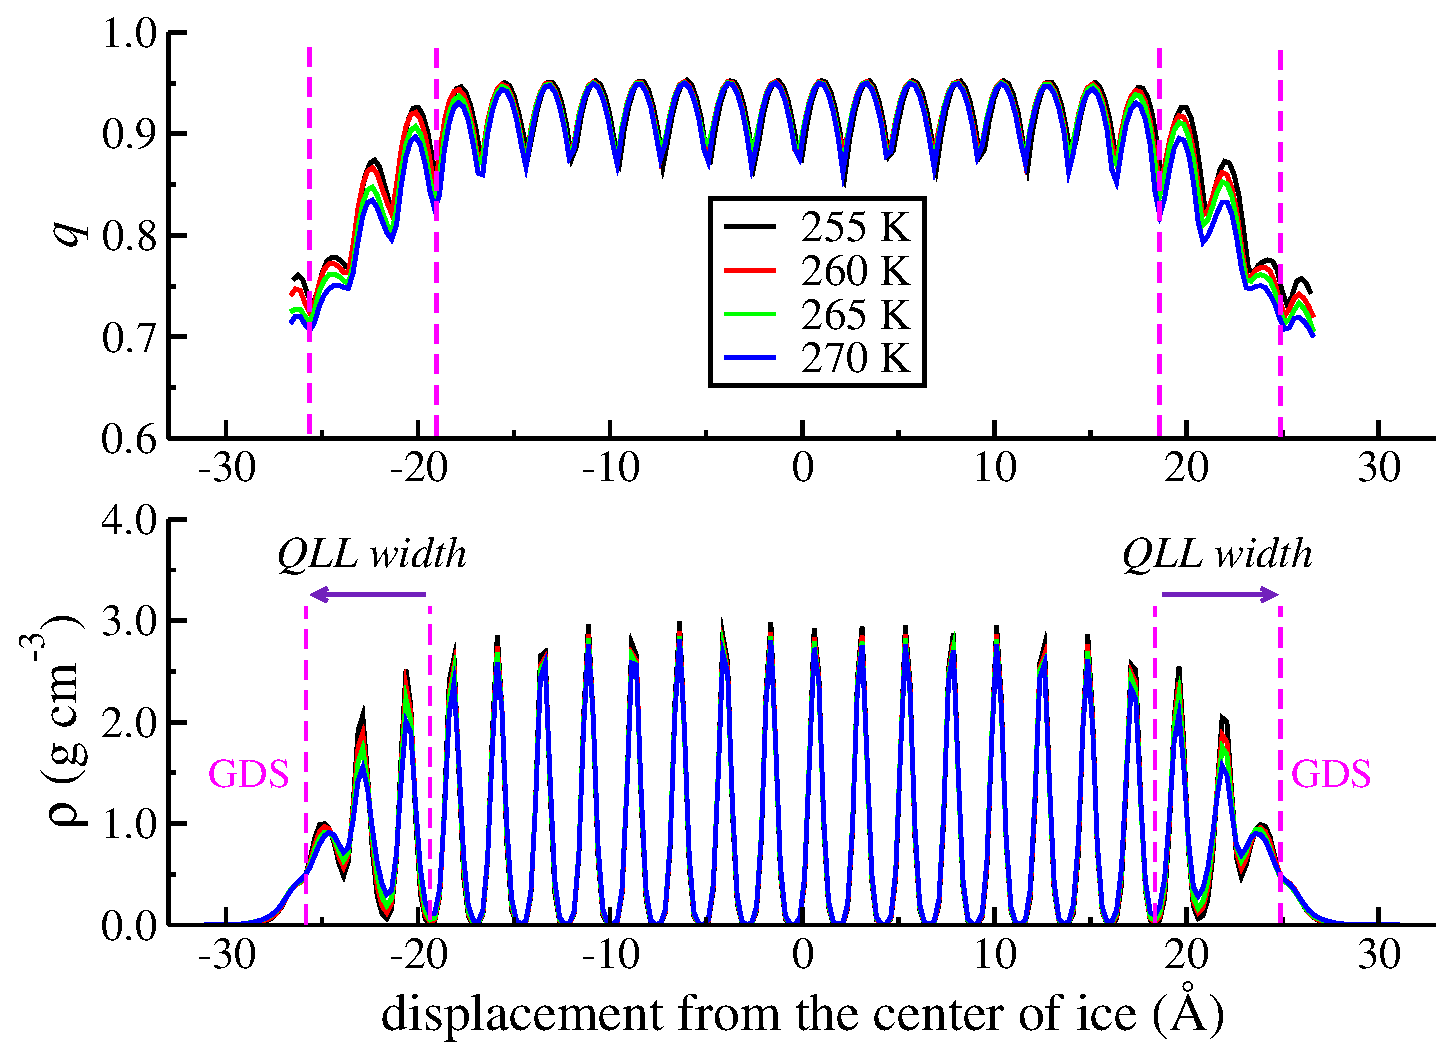
\includegraphics[width=\linewidth]{Figures/prism_qdens}
\caption{\label{fig:prism_rhoq} Panel description matches that of
  Figure \ref{fig:basal_rhoq}, but for the exposed prismatic
  ice-I$_\mathrm{h}$ crystal. }
\end{figure*}                

In the lower panel of Figure \ref{fig:basal_rhoq}, the local density
for the basal systems shows a formation of a QLL starting at
displacements of $d\sim\pm$ 15 \AA~ from the center of the ice. The
peaks at displacements greater than 18 \AA~ shows wetting of the
underlying crystal. That is, the density does not go to zero between
the crystal and liquid-like planes. Interior to this, the
characteristic bilayer of ice is observed in the twin peaks at each
plane of ice. Note the outermost peaks have lost this bilayer
feature, further indicating its liquid-like character. Estimates of
the QLL width can be obtained by taking the edge of the QLL to be
where the density goes to 0.5 $\mathrm{g}~\mathrm{cm}^{-3}$. Comparing
the density profiles for the four temperatures investigated, we
observe a greater extent of wetting of the underlying crystal for
warmer temperatures. Similarly, the height of the QLL peaks decreases
with warmer temperature, indicating a more liquid-like environment.

In the bottom panel of Figure \ref{fig:prism_rhoq}, the local density
for the prismatic systems indicates a quasi-liquid layer formation
around $d~\sim\pm$ 24. While the basal QLL density was found to be
$\rho~ \sim$~1.5 - 2.0 $\mathrm{g}~\mathrm{cm}^{-3}$, we observe
densities closer to 1.0 $\mathrm{g}~\mathrm{cm}^{-3}$ at the prismatic
surface. With increasing temperature, the same trend is observed at the
prismatic surface; at warmer temperatures the QLL's density comes
closer to that of the bulk liquid. We have estimated the width of the
QLL at each temperature investigated using the same density metric
described above. These estimates are shown in Figure
\ref{fig:qllWidth}.  

\begin{figure*}
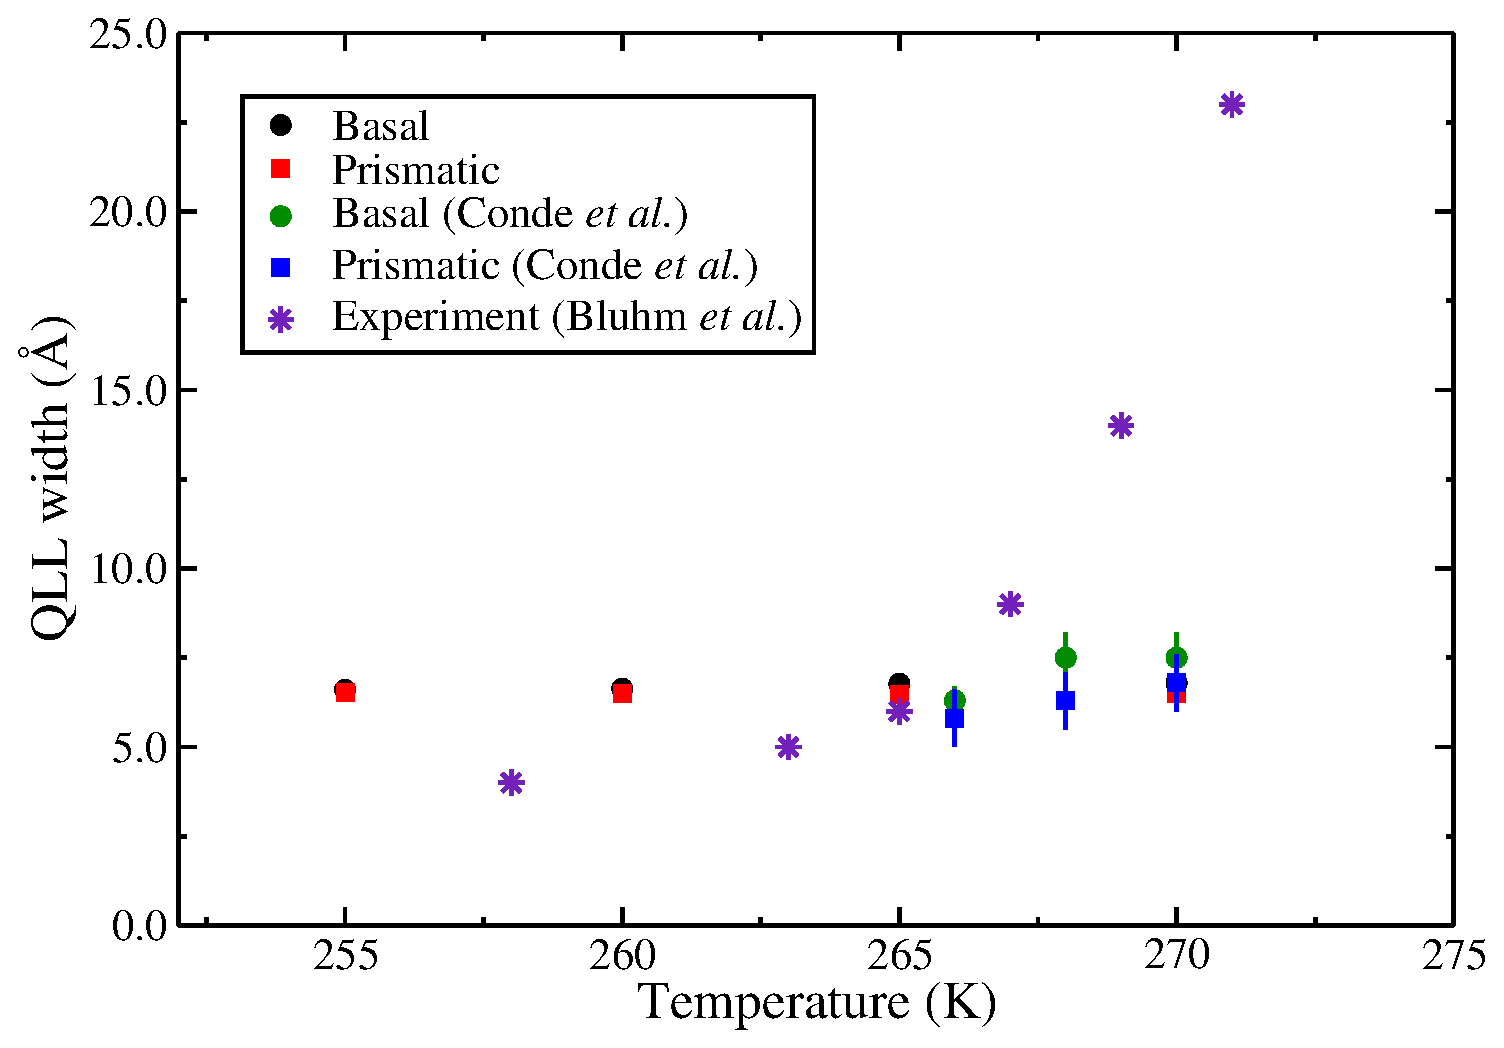
\includegraphics[width=\linewidth]{Figures/qllWidthT}
\caption{\label{fig:qllWidth} The temperature dependence of the width
  of the quasi-liquid layer as determined by density measures. The
  green and blue data are taken from Reference \cite{Conde2008}, and
  the purple data are taken from \cite{Bluhm2002}. }
\end{figure*}           

In Figure \ref{fig:qllWidth}, estimates for the basal (black) and
prismatic (red) interfaces show a relatively constant QLL width across
all four temperatures investigated, $w~\sim~6.7$~\AA. These results
agree well with values for the basal (green) and prismatic (blue) QLL
width obtained by Conde \textit{et al.} using the same
model.\cite{Conde2008} However, these estimates agree poorly with
near-edge X-ray absorption measurements of the basal surface taken by
Bluhm \textit{et al.}.\cite{Bluhm2002} Interestingly, no rigid,
non-polarizable water models are able to accurately capture the
divergence in the QLL width near the melting point,
$T_m = 273.15~\mathrm{K}$.\cite{Conde2008} This is not too surprising
considering the change in the dipole moment of individual water
molecules as their local environment changes from ice to QLL to vapor.

In the upper panels of Figures \ref{fig:basal_rhoq} and
\ref{fig:prism_rhoq} are the local tetrahedral order parameter
profiles through the interface. For the basal interface in Figure
\ref{fig:basal_rhoq}, we see the characteristic bilayer shapes in the
tetrahedrality profile. Interior to the ice, we observe $q$ values
close to 0.95, indicating a very tetrahedral environment. In the
region determined to be a QLL using density measures, the parameter
takes on values of 0.9 to 0.85. Beyond displacements of $d~\pm$~22
\AA~ from the center of the ice lies the vapor, and $q$ becomes small
and noisy due to the small population of molecules. The profile
presented in Figure \ref{fig:prism_rhoq} for the prismatic interface
appears very similar to that of the basal interface. It is interesting
to note, that since the tetrahedral order parameter depends on
neighboring molecules, it indicates that the crystal plane interior to
the QLL layer also deviates from bulk-like environments. This stems
from the outer layer being structured in a less tetrahedral
manner. While this could indicate that this first interior layer
should also be denoted as a QLL, perhaps it is more appropriate to
name this layer as a quasi-solid layer (QSL).


\section{Viscosity of the Quasi-Liquid Layer}

According to kinetic theory, the diffusion constant, $D$, can be
related to the mobility ($\mu$) of a particle and the temperature,
$T$.
\begin{equation}
D = \mu k_B T
\end{equation}
The mobility is often described as the ratio of the particle's
terminal velocity to an applied force. A specialized form of
this relation relates the diffusion constant to the shear viscosity
($\eta$) of the fluid.
\begin{equation}\label{eq:stokes-einst}
D = \frac{k_BT}{4\pi \eta r}
\end{equation}
Equation \eqref{eq:stokes-einst} was first derived by Einstein to
determine the diffusion constant for a ``Stokes'' particle of radius
$r$ undergoing Brownian Motion. 

\subsection{The Reduced Viscosity of the Quasi-Liquid Layer}
A reduced viscosity of the quasi-liquid layer can be obtained by
relating the viscosity of the QLL to that of a supercooled bulk
liquid at the same temperature.
\begin{equation}\label{eq:eta*}
\eta^* = \frac{\eta^{\mathrm{qll}}}{\eta^{\mathrm{bulk}}}
\end{equation}

In order to compute estimates of the reduced viscosity of the QLL from
Equation \eqref{eq:eta*}, spatially resolved three dimensional
diffusion constants were computed in 1 \AA~bins along the dimension
normal to the ice surface.
\begin{equation}\label{eq:yDiff}
D(y) = \frac{1}{6t} \langle | \mathbf{r}_i(t) - \mathbf{r}_i(0) |^2
\delta(y_i(0) - y)  \rangle 
\end{equation}
Once obtained, it is a simple matter to scale each set of spatially
resolved diffusion coefficients by the diffusion coefficient for the
supercooled bulk liquid at the same temperature to obtain Figure
\ref{fig:basal_eta0} for the basal interface and Figure
\ref{fig:prism_eta0} for the prismatic interface. 

\begin{figure*}
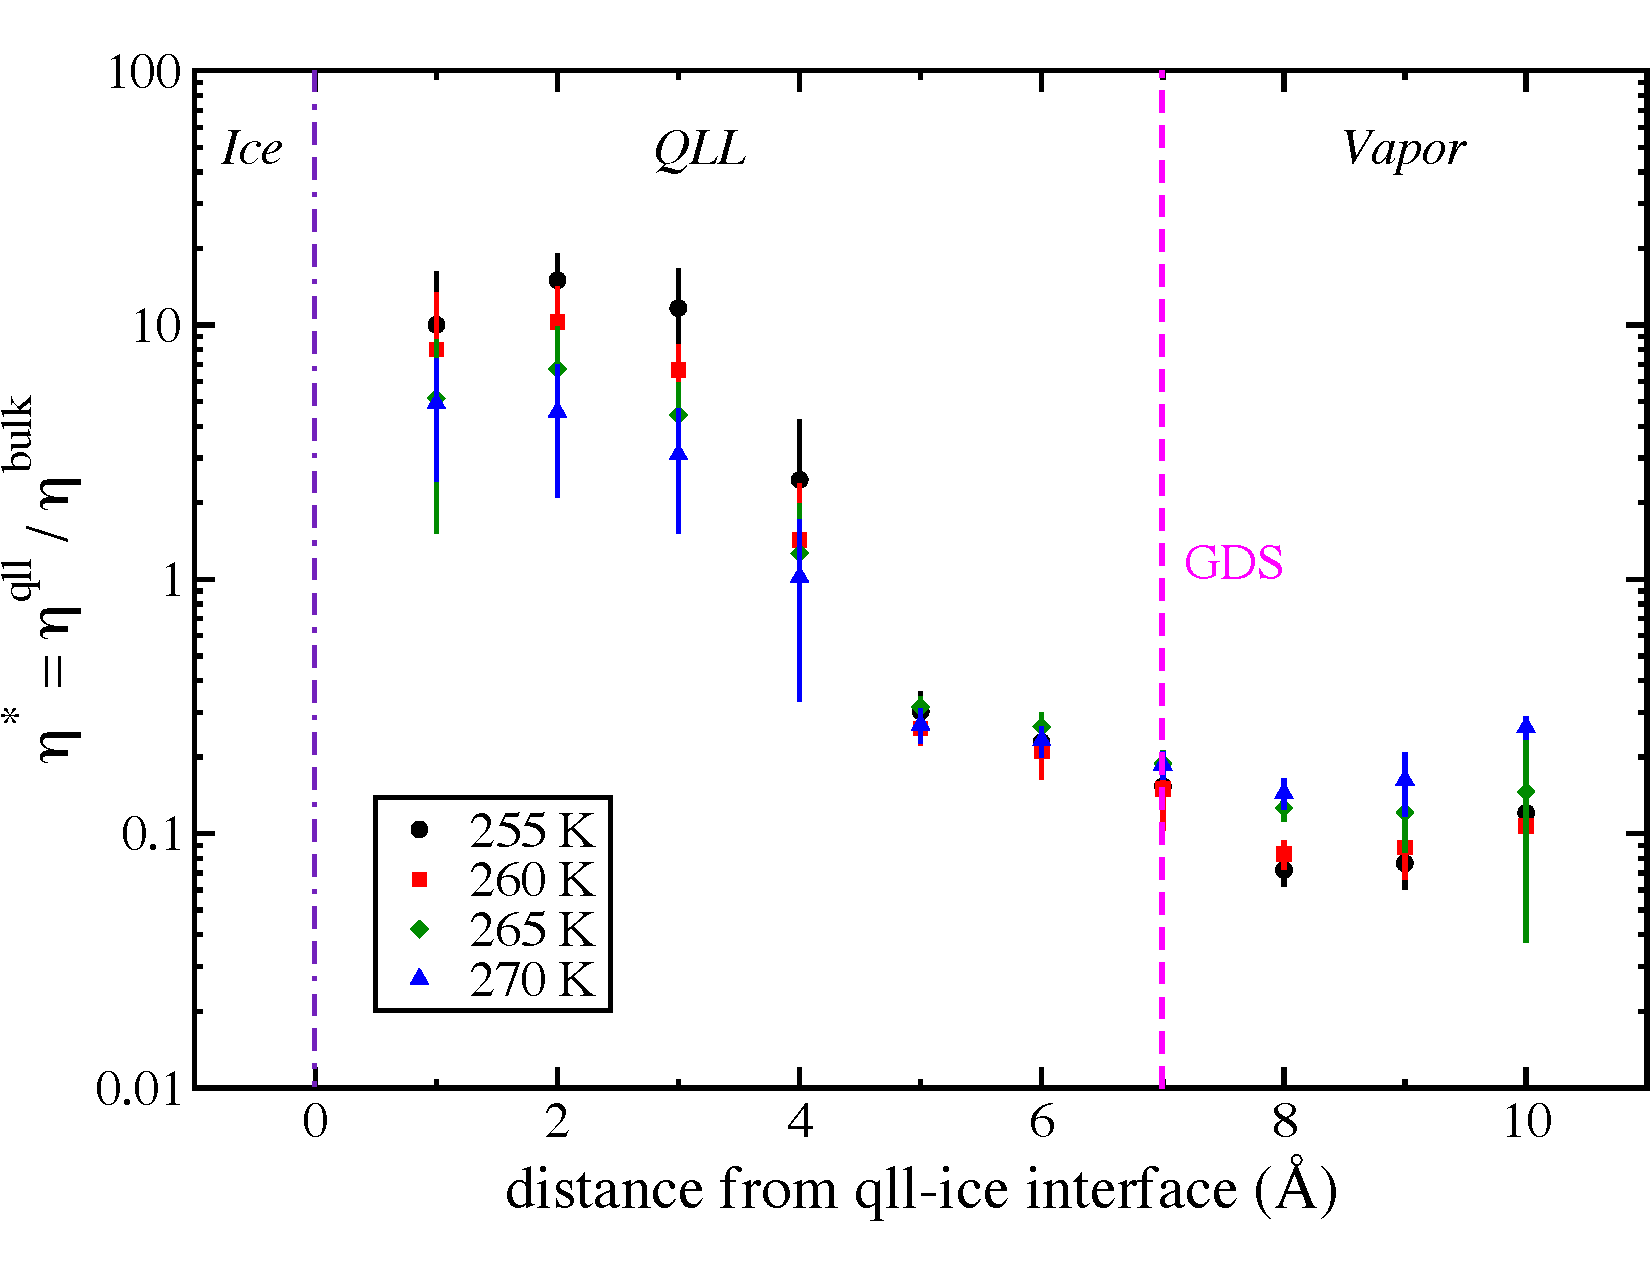
\includegraphics[width=\linewidth]{Figures/basal_eta0}
\caption{\label{fig:basal_eta0}The spatially resolved reduced
  viscosity at the basal surface of ice-I$_\mathrm{h}$. The Gibbs
  dividing surface between the QLL and the vapor is indicated as a
  vertical magenta line.}
\end{figure*}                

\begin{figure*}
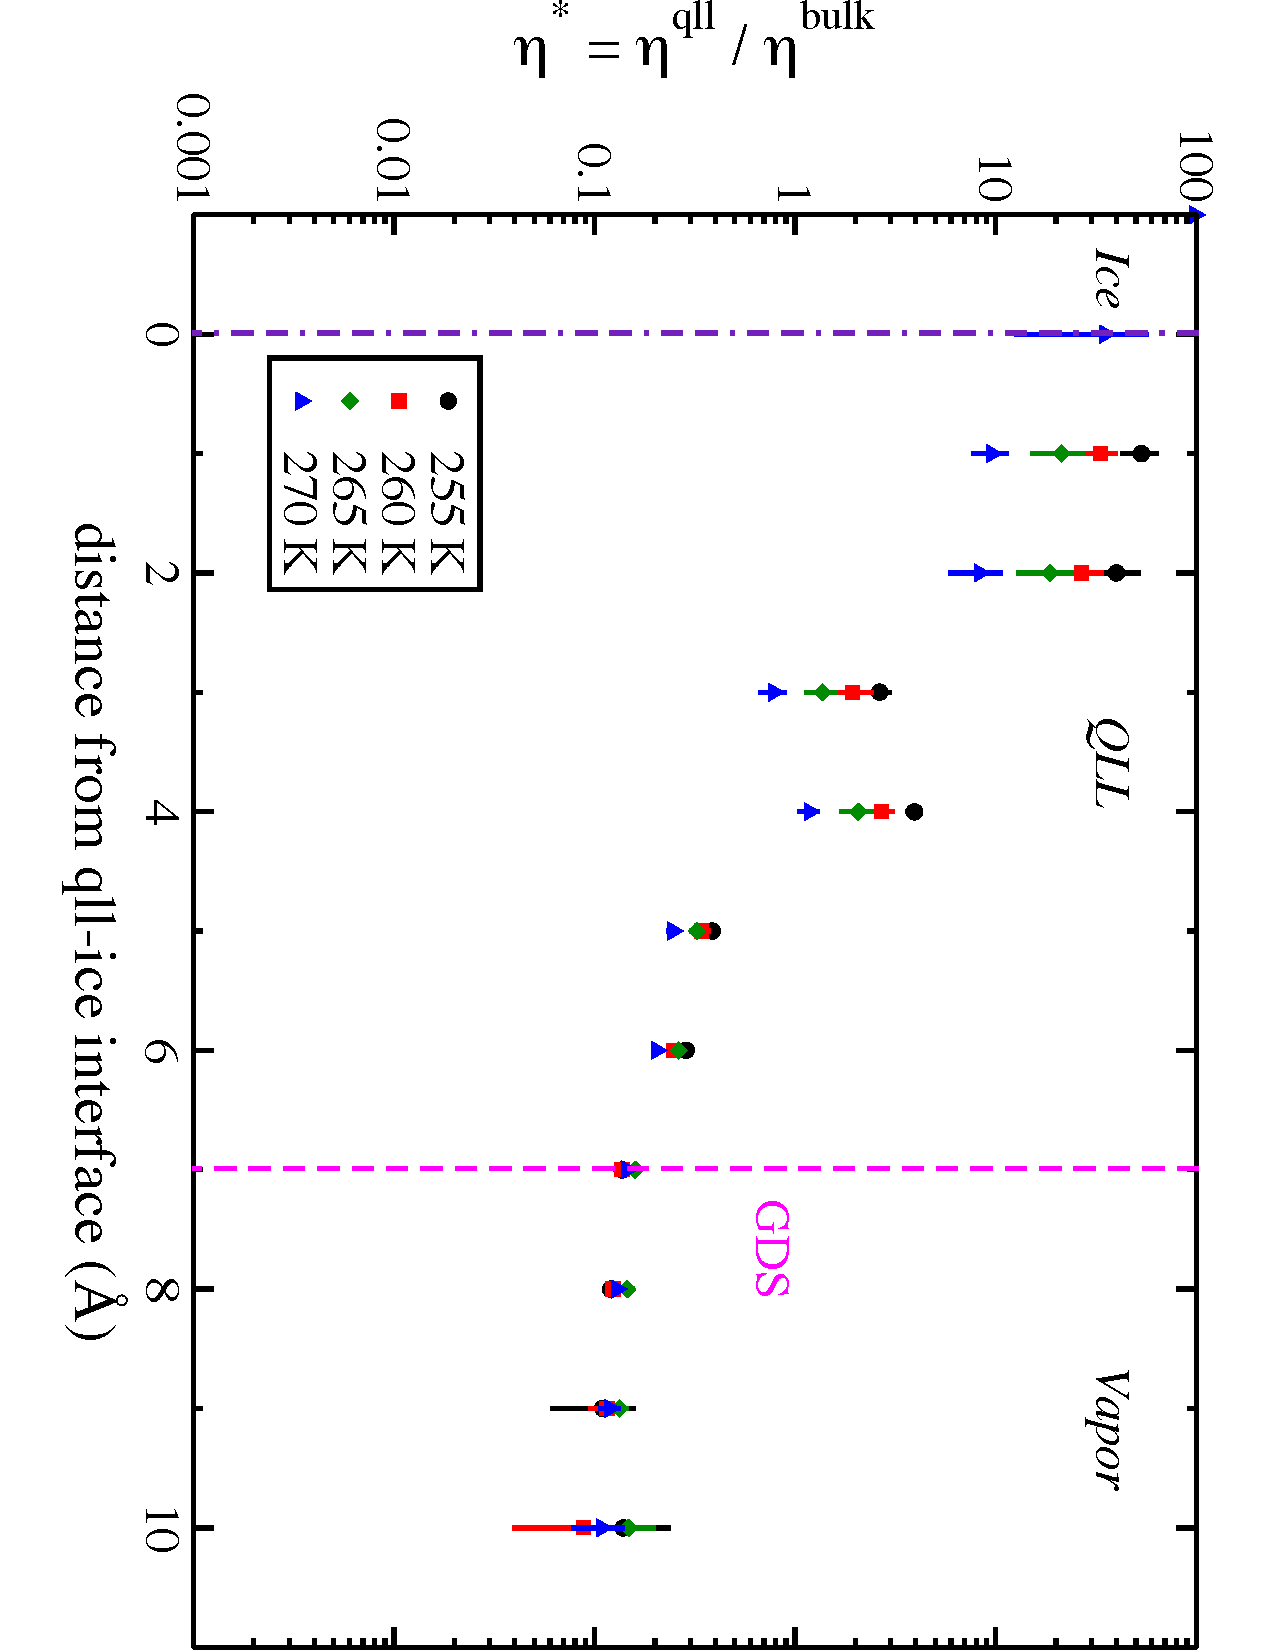
\includegraphics[width=\linewidth]{Figures/prism_eta0}
\caption{\label{fig:prism_eta0} Panel description matches that of
  Figure \ref{fig:basal_eta0}, except for the prismatic surface of
  ice-I$_\mathrm{h}$.}
\end{figure*}                

In Figures \ref{fig:basal_eta0} and \ref{fig:prism_eta0}, we see close
to the ice the reduced viscosity is quite large, $\eta^* \sim 10$ to
$\eta^* \sim 100$, depending on the interface and temperature. Close
to the Gibbs dividing surface between the QLL and the vapor (magenta
vertical line), the reduced viscosity is close to 0.1 for both
interfaces. These results indicate that the viscosity of the QLL
varies drastically with distance from the ice surface. Using these
reduced viscosities along with a temperature dependent model for the
shear viscosity of the bulk supercooled liquid, we could obtain
estimates for the shear viscosities of the QLLs studied here.
           
\subsection{Shear Viscosity of Supercooled Liquid}
We have performed velocity shearing and scaling reverse
non-equilibrium molecular dynamics simulations in order to obtain a
temperature dependent model of the shear viscosity of supercooled bulk
liquid water. A liquid box containing $16,000$ TIP4P/Ice water
molecules with dimensions $\mathrm{L_x} = 51.22~\mathrm{\AA}$,
$\mathrm{L_y} = 51.22~\mathrm{\AA}$, and
$\mathrm{L_z}=200.87~\mathrm{\AA}$ was subjected to simultaneous
kinetic energy and momentum fluxes. This resulted in concurrent thermal
and velocity gradients across the $z$-dimension of the simulation
box. The velocity profile was fit with a quadratic regression, and an
analytic derivative with respect to the $z$ gave
$(\frac{\partial V_x}{\partial z}$). Together with the imposed
momentum flux, the shear viscosity is easily obtained.
\begin{equation}\label{eq:viscosity}
  j_{z}(p_{x}) = -\eta \big(\frac{\partial v_{x}}{\partial z}\big)
\end{equation}
The temperature gradient through the system was fit with a linear
regression. Using this regression, the local temperature for each
$\eta$ was obtained.  

The resulting $\eta$ values were fit with the Vogel Fulcher Tammann model
for predicting the shear viscosity of polymers and other liquids which
exhibit a glass transition temperature ($T_g~\sim~136~\mathrm{K}$ for
water). 
\begin{equation}\label{eq:WLF}
\eta (T) = \eta_0 \exp \Bigg({\frac{B}{T-T_0}}\Bigg)
\end{equation}
Here, $\eta_0$ and $B$, are fit parameters describing the infinite
temperature viscosity and the thermal energy required to change the
viscosity, respectively. $T_0$ is an empirical parameter, typically
taken to be the glass transition temperature ($T_g$).  With this it is
possible to estimate the temperature dependence of the shear viscosity
by knowing it only at one data point. Our data and resulting fit can
be seen in Figure \ref{fig:etaT}.
\begin{figure*}
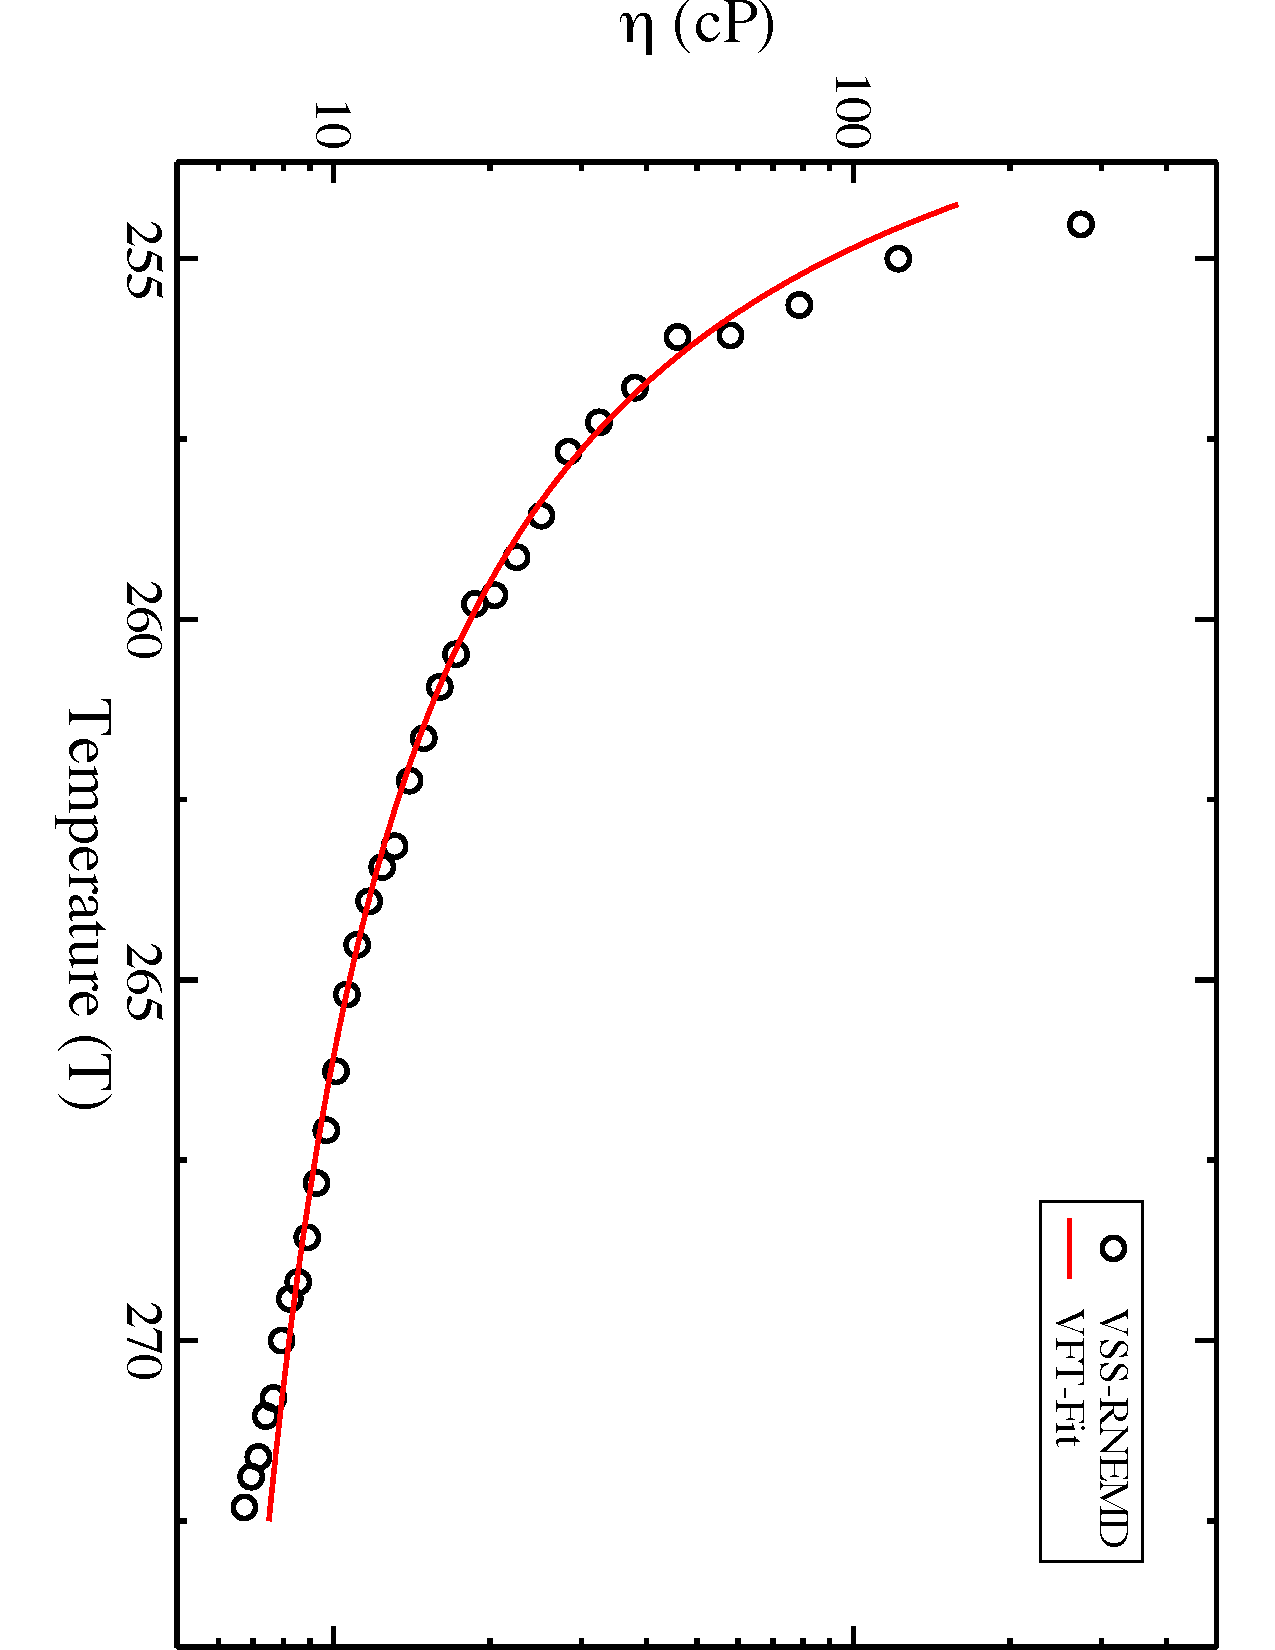
\includegraphics[width=\linewidth]{Figures/bulkVFT}
\caption{\label{fig:etaT} The shear viscosity $\eta$ of supercooled
  liquid water as a function of temperature. The black circles are
  data computed from a single VSS-RNEMD simulation with simultaneous
  kinetic energy and momentum fluxes, the red curve is a fit described
  by the Vogel Fulcher Tammann model.}
\end{figure*} 
Querying the fit at the four temperatures the ice surfaces were
investigated at, we can obtain reasonable estimates of the shear
viscosity for the supercooled bulk liquid. These values are reported
in Table \ref{tab:bulkVisco}.
   

\begin{table}[h] \centering \caption{SHEAR VISCOSITY OF THE
    SUPERCOOLED BULK LIQUID\label{tab:bulkVisco}}
\begin{tabular}{cc}
\hline
\hline
 Temperature & $\eta$ \\
\hline
270 & 8.2 \\
265 & 10.7 \\
260 & 18.3  \\
255 & 85.5 \\
\hline
\hline
\end{tabular}
\begin{flushleft}
  Temperatures are given in K, and shear viscosities are reported in
  cP.
\end{flushleft}
\end{table}


\subsection{The Shear Viscosity of the Quasi-Liquid Layer}
Using the reduced viscosities of the quasi-liquid layers and the
temperature dependent model for the shear viscosity of bulk
supercooled liquid, we have estimated the shear viscosity of the QLLs
at the basal and prismatic surfaces of ice-I$_\mathrm{h}$.
\begin{equation}\label{eq:qllT}
\eta^{\mathrm{qll}}(T) = \frac{\eta^{\mathrm{qll}}}{\eta^{\mathrm{bulk}}}\eta^{\mathrm{bulk}}(T)
\end{equation}
In Figure \ref{fig:qllEta}, the spatially resolved shear viscosity of
the basal (bottom panel) and prismatic (upper panel) interfaces are
reported. Close to the ice, we find shear viscosities between
$\eta(270~\mathrm{K}) = 35~\mathrm{cP}$ and
$\eta(255~\mathrm{K}) = 1100~\mathrm{cP}$ for the basal interface, and
between $\eta(270~\mathrm{K}) = 71~\mathrm{cP}$ and
$\eta(255~\mathrm{K}) = 5800~\mathrm{cP}$ at the prismatic
interface. At the QLL / vapor interface, the viscosity becomes
invariant to the presented crystal facet, and values of
$\eta(255~\mathrm{K}) = 16~\mathrm{cP}$ to
$\eta(270~\mathrm{K}) = 1~\mathrm{cP}$ are observed at both
interfaces. Between these two regions, we observe a continuous
distribution of $\eta^{\mathrm{qll}}(T)$ for both of the crystal
facets investigated. 

\begin{figure*}
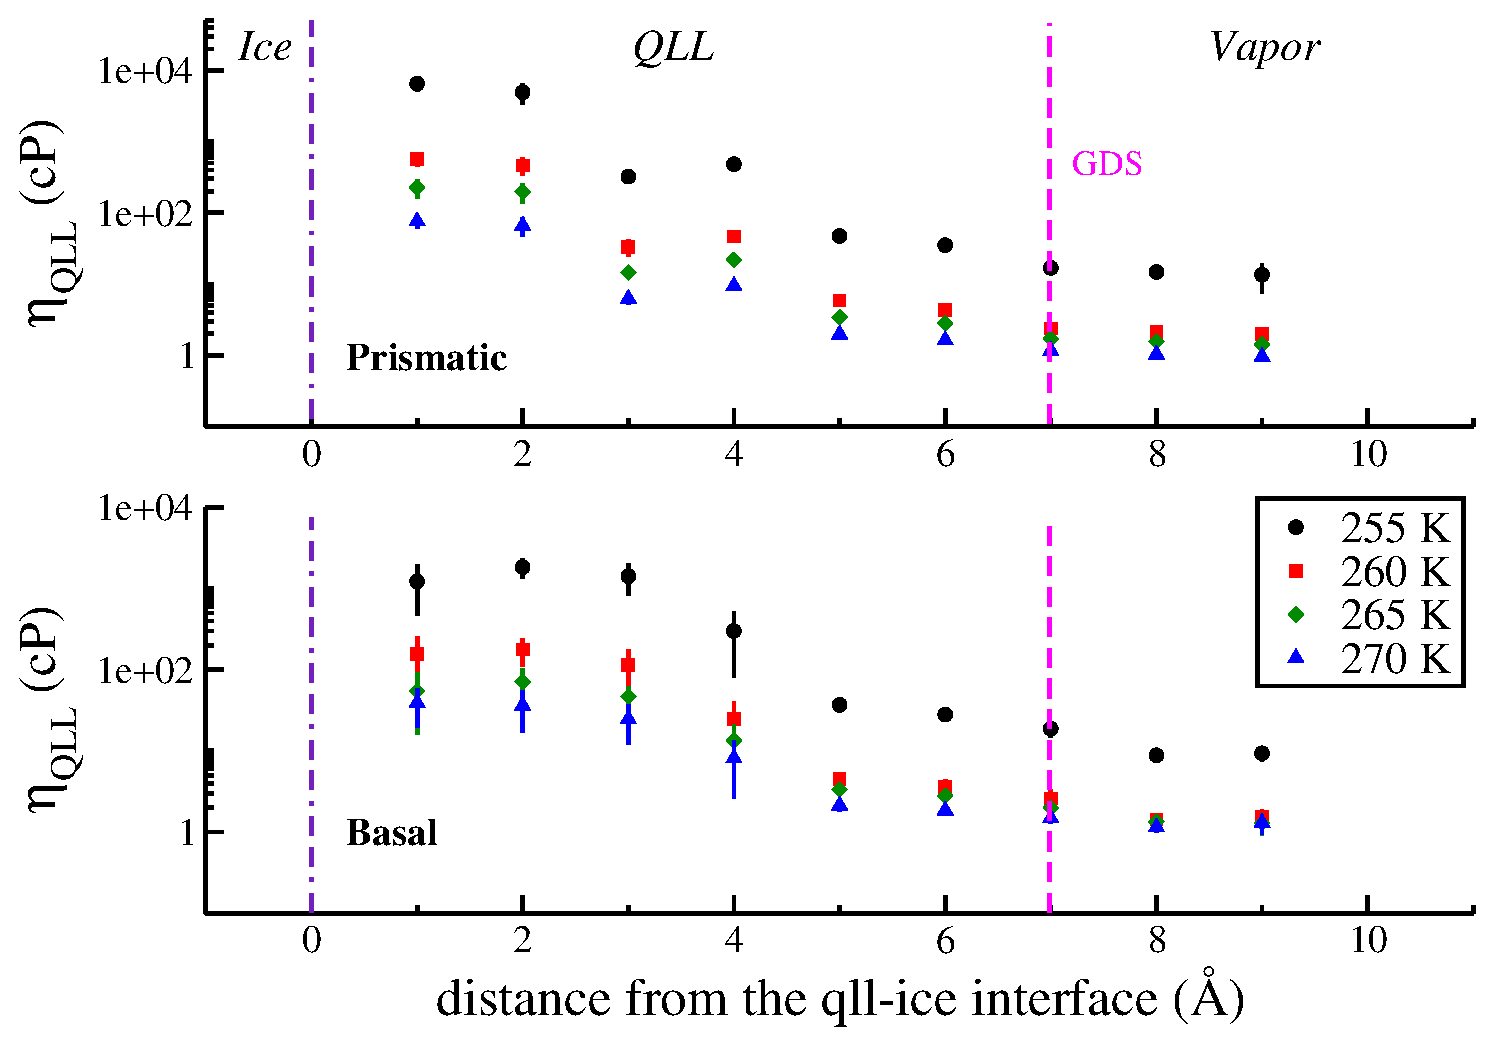
\includegraphics[width=\linewidth]{Figures/qllEta}
\caption{\label{fig:qllEta}The spatially resolved shear viscosity of
  the quasi-liquid layer at the basal (lower) and prismatic (upper)
  surfaces of ice-I$_\mathrm{h}$. The vertical indigo line helps guide
  the eye between the ice and the QLL interface, and the magenta
  vertical line indicates the Gibbs dividing surface between the QLL
  and the vapor.}
\end{figure*} 

We attempted to compute the shear viscosity of the quasi-liquid layers
in a second way. Using VSS-RNEMD \cite{Kuang2012}, a shear stress was
applied only to molecules in the QLLs. The VSS-RNEMD exchange regions
were defined to incorporate molecules from both the top and bottom
interfaces, and partitioning between the vapor, QLLs, and the ice
surfaces was performed using the local tetrahedral order parameter of
the water molecules. However, application of the VSS-RNEMD moves
resulted in non-linear behavior in the velocity distributions of the
QLLs. The surface premelt layers were found to couple more strongly with the
underlying ice than the neighboring QLL, resulting in dissipation of
the velocity ``kicks'' into the ice instead of in the surface
premelt. Due to this, we were unable to resolve shear viscosities
using the VSS-RNEMD method.



\section{Discussion}

\subsection{Width of the Quasi-Liquid Layer}
Conde \textit{et al.} investigated water model dependence on the
formation of the quasi-liquid layer at the vapor exposed basal,
prismatic, and secondary prismatic surfaces of
ice-I$_\mathrm{h}$.\cite{Conde2008} They established a cutoff value in
the local tetrahedral order parameter, $q_t$, to denote molecules as
being ice-like or liquid-like. Using this, they estimated QLL widths
to be $w~\sim$~5 - 10~\AA~ for the TIP4P/Ice model over the range of
temperatures investigated here. These results agree well with our
density based estimates of the QLL width, of $w~\sim~6$~\AA~for both
the basal and prismatic facets.

As described in Chapter \ref{chap:Methods}, the basal and prismatic
surfaces used in this study exhibit proton ordering at the surface of
the crystal. This was chosen to reproduce sum frequency generation
spectroscopy which indicated proton ordering at the basal surface of
ice. Conversely, the ice surfaces simulated by Conde \textit{et al.}
presented disordered protons. Our results here indicate that the
proton-ordering at the basal and prismatic surfaces of
ice-I$_\mathrm{h}$ do not significantly alter the width of the QLL as
compared to proton disordered surfaces.  Furthermore, Conde
established that the SPC/E, TIP4P, TIP4P/2005, and TIP4P/Ice models
estimated QLLs of similar thickness, when compared to the relative
undercooling temperature of the model.\cite{Conde2008} Given that our
estimates of the thickness of the QLL agrees with that of Conde, we
believe our estimates should be robust for other water models as well,
but we have no evidence of this.

Neshyba \textit{et al.} investigated sublimation and deposition of
water molecules at the ice / vapor interface.\cite{Neshyba2009} They
also observed the formation of a QLL while using the NE6
model\cite{Nada2003a} at 250 K (T$_\mathrm{m}$ - 48 K for the NE6
model), and discriminated the QLL molecules by their intermolecular
potential energy. Doing so, they designated two separate QLLs, which
we have described as a single QLL here. They distinguish an outer QLL
which contains roughly 8\% of the total molecules, and an inner, more
crystalline QLL containing the remaining 92\%. 

As we observed in Figures \ref{fig:basal_rhoq} and
\ref{fig:prism_rhoq}, the value of the density and tetrahedrality in
the QLL is very local. We observe, that the structure and dynamics of
the water molecules vary drastically from the vapor to the QLL / ice
interface, and assigning an average value for any of the parameters
investigated here for each of the QLLs studied would be improper.


\subsection{Anisotropic Diffusion of the Quasi-Liquid Layer}
Pfalzgraff \textit{et al.}\cite{Pfalzgraff2011} and later Gladich
\textit{et al.}\cite{Gladich2011,Gladich2015} observed anisotropic
diffusion of the QLL on the prismatic, 14\degree~ pyramidal, and
secondary prismatic surfaces of an ice-I$_\mathrm{h}$ crystal. This
behavior was prominent at colder temperatures (60 to 40 K of
undercooling) where the QLLs were thin and the water contributing to
the QLL is significantly influenced by the underlying crystal
structure. Since the underlying crystal exhibits an anisotropic
potential energy surface for movement of the QLL water molecules, the
resulting diffusion is biased by the directional dependent
energetics. At warmer temperatures and correspondingly thicker QLLs,
isotropic diffusion is recovered.

Here, we have computed one dimensional diffusion constants for small
($\delta y$) bins normal to the basal and prismatic ice surfaces.
\begin{equation}\label{eq:1dDiff}
D_i = \frac{1}{2t} \langle | {r}_i(t) - {r}_i(0) |^2
\delta(y(0) - y)  \rangle 
\end{equation}
Taking the ratio of $D_x / D_z$, where $x$ is towards the secondary
prismatic face on the basal surface, and towards the basal face on the
prismatic surface, we have obtained the results shown in Figure
\ref{fig:dxdz}. At the basal surface (lower panel), we observe
isotropic diffusion for all four temperatures investigated. This
agrees well with Gladich \textit{et al.},\cite{Gladich2011} although
they conjectured that at extreme undercooling and correspondingly
sufficiently thin QLL, the basal surface may display anisotropic
diffusion relative to its six-fold symmetry.

\begin{figure*}
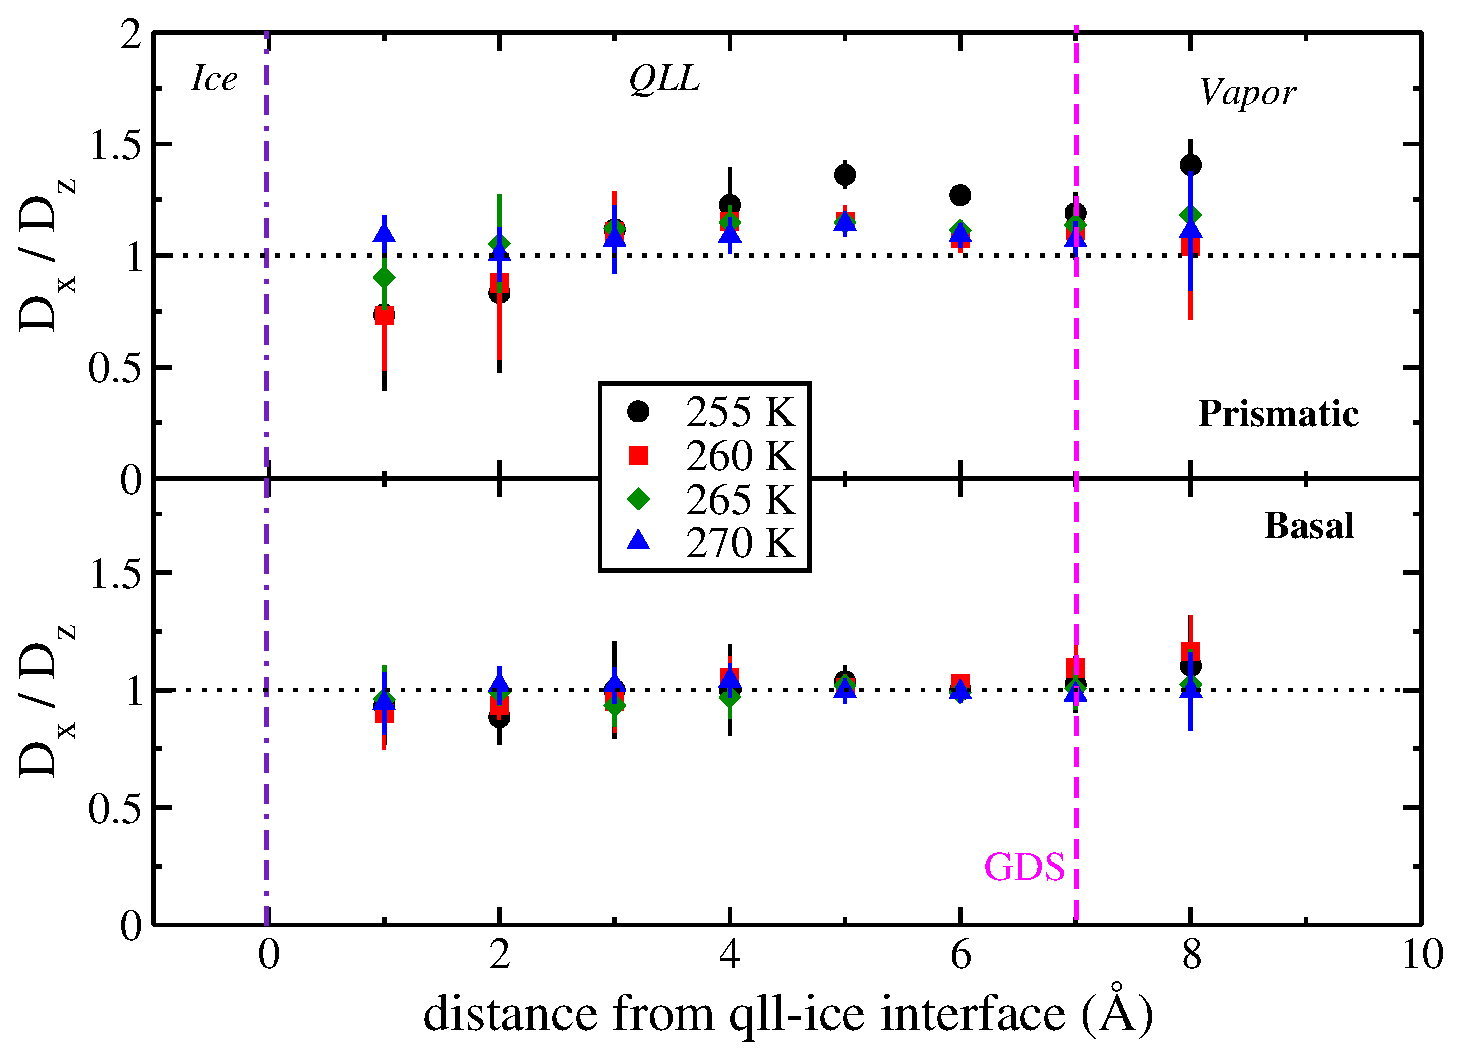
\includegraphics[width=\linewidth]{Figures/rd}
\caption{\label{fig:dxdz}The ratio of one dimensional diffusion
  constants for the basal (lower) and prismatic (upper)
  surfaces. Details about which crystal face the axis point towards is
  given in text.}
\end{figure*} 

Conversely, we observe anisotropic diffusion at the prismatic surface
in the top panel. Close to the ice crystal, the large error bars do
not allow us to clearly resolve if the diffusion is biased. At
distances between 3 and 6 \AA~away from the ice / QLL interface, we
clearly see a bias for diffusion along the $x$-dimension. This result
challenges the theory of Gladich \textit{et al.}, in which they
proposed anisotropic diffusion occurring close to the ice surface. In
addition, they predicted that isotropic diffusion should be recovered
by 30 degrees of undercooling, although we have observed anisotropic
diffusion up to 1 or 2 degrees of undercooling with the TIP4P/Ice
model. We have computed spatially resolved one dimensional diffusion
constants, however, Gladich computed an average diffusion constant for
the entire QLL. This may explain some of the differences observed
between their investigations and our presented results.

\subsection{Quasi-Liquid Layer Viscosity}
Comparing the spatially resolved shear viscosities of the QLLs with
the values obtained for supercooled liquid water in Table
\ref{tab:bulkVisco}, we see that the bulk liquid agrees within error
with the QLLs at approximately 4 - 5~\AA~ from the surface, for both
the basal and prismatic surfaces. At distances closer to the ice
surface, the shear viscosities of the QLLs are much greater than that
of the bulk liquid, and similarly at distance greater than 4 - 5~\AA~
from the ice / QLL interface the shear viscosity drops below that of
the bulk.

There are a few reasons why we see disagreement between the
supercooled liquid and the QLL viscosities near the ice or vapor
phases. Close to the ice, the QLL water experiences a confined space
and therefore the barrier for movement becomes larger. Similarly, the
close proximity to the ice surface may cause a templating of the
liquid, as the static potential energy surface exhibited by the ice
surface could also increase the barrier for movement. Close to the
vapor, the smaller values of $\eta$ may be due to the open
environment.  In contrast, the bulk liquid at the same temperature is
subjected to a moderate confined space, somewhere between the
excluded volume due to the ice surface, and that of the open vapor
phase. This may explain why the shear viscosity in the middle of the
QLLs agrees with that of the bulk. 

A second possibility is that the local structure of the molecules in
the QLL is different from that of the bulk liquid. From the top panel
of Figure \ref{fig:gofrQ}, the supercooled bulk liquid's
tetrahedrality distribution has a maximum of about $q \sim$~0.89, and
is observed to decrease slightly with increasing
temperature. Conversely, in the top panels of Figure
\ref{fig:basal_rhoq} and \ref{fig:prism_rhoq}, $q$ for the QLLs varies
drastically with distance from the ice / QLL interface. At distances
of $d~\sim~4 - 5$~\AA~ from the ice / QLL interface, the
tetrahedrality of the QLLs agrees reasonably with the supercooled bulk
liquid. This may also help explain why the local shear viscosity at
this distance from the ice / QLL interface agrees with the bulk liquid
of the same temperature. 

Lastly, comparing the shear viscosities close the ice / QLL interface
for the basal and prismatic surfaces, we see that at all temperatures
investigated
$\eta_{\mathrm{prism}}^{\mathrm{QLL}}~>~\eta_{\mathrm{basal}}^{\mathrm{QLL}}$. This
result agrees well with our calculations of the friction coefficients
in Chapter \ref{chap:Friction}, where we found
$\kappa_{\mathrm{prism}}~ >~\kappa_{\mathrm{basal}}$. Conversely,
close to the QLL / vapor interface,
$\eta_{\mathrm{prism}}^{\mathrm{QLL}}$ and
$\eta_{\mathrm{basal}}^{\mathrm{QLL}}$ come into agreement, and are
much smaller, varying from $\eta = 17.5$~cP to $\eta = 1.7$~cP. We
conclude that the small coefficients of friction commonly associated
with ice surfaces to be due to the small shear viscosity found for
water molecules near the QLL / vapor interface. 


% Similarly, Dehaoui
% \textit{et al.} have measured the viscosity of supercooled water down
% to -34\degree C without freezing the liquid.\cite{Dehaoui2015} There
% have been suggestions that Equation \eqref{eq:stokes-einst} breaks
% down at temperatures close to T$_\mathrm{g}$, the glass transition
% temperature, implying that the translational diffusion and the shear
% viscosity of the liquid become decoupled.


% As seen in Figure \ref{fig:qll-rhoq}, the QLLs at the surface of the
% basal and prismatic crystals form a bilayer. Following Neshyba
% \textit{et al.}, we denote the following definitions; molecules within
% the ice are labeled as $\mu_{i}$, where each $i$ denotes a unique
% density peak in the ice, molecules in the QLL layer closer to the ice
% are labeled as $\epsilon_{2}$, and molecules in the outer portion of
% the QLL bilayer are labeled as $\epsilon_{1}$.\cite{Neshyba2009} Due
% to their relative distances from the underlying crystal, molecules
% within layers $\epsilon_{2}$ and $\epsilon_{1}$ experience vastly
% different local environments. Water molecules within $\epsilon_{2}$
% located closer to the ice experience significantly more drag than
% those closer to the vapor. Therefore, we expect a noticeably different
% sheer viscosity for the molecules located in $\epsilon_{2}$ and
% $\epsilon_{1}$. 


% % In a recent review of Ice Surfaces, Mary Jane Shultz posed numerous
% % open questions about the qll, such as what is the growth mechanism,
% % relative energies of various faces are not well understood, what is
% % the impact of face termination on ice surface energy and reactivity,
% % what defintion is relevant for the qll, at what temperature does the
% % qll from, what is the nature of the qll?

% 2017 PNAS paper by M. Alejandra Sanchez \textit{et al.} provides
% experimental (surface-specific vibrational sum frequency generation
% spectroscopy)  and theoretical (molecular dynamics simulations with
% the TIP4P/Ice model)
% evidence that the qll formation occurs
% bilayer-by-bilayer. Observed for the basal face and the secondary prism. 

% % Determination of Surface Tension-to-Shear Viscosity Ratio for
% % Quasi-liquid layers on Ice Crystal Surfaces.
% %   K. Murata, H. Asakawa, K. Nagashima, Y. Furukawa, G. Sazaki
% %   PRL 115 (2015) 256103
% Using laser confocal microscopy in conjunction with an inverted
% optical microscope, Murata \textit{et al.} have recently measured the
% characteristic-velocity (\textit{i.e.} the surface tension-to-shear
% viscosity ratio) of two distinct wetting morphologies of QLLs on the
% basal surface of ice at -0.2 degrees Celcius and a pressure of 578.9
% Pa.\cite{Murata2015} They observed a partial wetting QLL, described as
% a bulk liquid droplet (BLD), as well as a complete wetting state,
% described as a thin liquid layer (TLL). The characterstic-velocity of
% the BLDs was determined from relaxation modes of their contact lines,
% which was observed to decay with single exponential behavior according
% to
% \begin{equation}
% u_q = u_q(0) exp\Bigg(-\frac{V^* \theta^3 q}{3l}t\Bigg)
% \end{equation}
% where $q$ is the wave vector for the perturbing mode for the
% relaxation of the amplitude of the contact line and $u_q(0)$ being the
% initial amplitude of the mode. Here, $V^* = \gamma / \eta$ is the
% characteristic velocity and $\theta$ is the contact angle the BLD makes
% with the ice surface ($\sim$ 2 degrees). Lastly, the logarithmic factor
% $l=ln(L/a)$ is a cutoff parameter which helps avoid
% singularities. From this fit, they obtained $V^* = 2 \pm 1$ m/s, which
% is about an order of magnitude smaller than that of bulk water, 42.21
% m/s.

% Murata \textit{et al.} also investigated the spreading dynamics of the
% BLD-QLLs, during the transformations to TLL-QLLs. The radii of the
% spreading BLD-QLLs were fit to a power law
% \begin{equation}
% r = L (\frac{4S}{3Ll \eta})^{1/4}(t+t_0)^{1/4}.
% \end{equation}
% Here, $S$ is the spreading coefficient, and $t_0$ captures the initial
% state of the droplet. As the QLL transitions from the BLD
% drpolet-shape to the TLL pancake-shape, the volume must be
% conserved. From this conservation, Murata \textit{et al.} estimated
% the thickness of the TLLs as 9 $\pm$ 3 nm.

% Lastly, Murata \textit{et al.} have obtained the characteristic
% velocity of the TLLs in the same way as the BLDs. However, here the
% hydrodynamic dissipation is not located at the wedge of the droplet
% like in the BLD case, but instead the dissipation occurs within the
% fluid of the pancake-shape object itself. Due to this, a slightly
% different expression for the viscous force must be used, and the
% resulting characteristic velocity was found to be $V^* = 0.2 \pm 0.1$
% m/s, about 200 times smaller than that of bulk water. This seems to
% imply a dependence on the characteristic velocity to the QLLs contact
% area and distance from the surface. The BLD droplet-shaped QLLs (where
% the QLL is only partially wets the surface and a larger amount of the
% QLL resides further from the surface), were found to have a
% characteristic velocity of about an order of magnitude larger than the
% more completely wetting state, where more of the QLL resides closer to
% the surface.

% It is interesting to note that the surface tension of the BLD/air
% interface ($\gamma_t$) is approximately equal to the TLL/air interface
% surface tension ($\gamma_b$), as there is observed coexistence of both
% forms of QLLs at the same time. Therefore, the discrepancy in $V^*$
% can be primarily attributed to the shear viscosity of the QLL phase.
 
% % end Murata2015


% Discuss widths of qll by experimental groups. Probing different
% measures of the qll gives different widths at different
% temperatures. Give a quick summary of the kinds of experiments and
% what their findings were for qll widths.




% Break down of stoke's-einstein relation for viscosity. \cite{Chen2006,
%   Tarjus1995,Bordat2003,Kumar2007}


% % The thickness of a liquid layer on the free surface of ice as
% % obtained from computer simulation. M.M.Conde, C.Vega, A.Patrykiejew
% % JCP 129, 014702 (2008)
% %Outstanding references and background
% Molecular dynamics simulations of ice-I$_\mathrm{h}$ with a free
% surface were performed using the SPC/E, TIP4P, TIP4P/Ice, and
% TIP5P/2005 water models. The basal, prismatic, and secondary prismatic
% surfaces exposed to vacuum were analyzed. Conde \textit{et al.}
% observed that the thickness of the liquid like layer that develops on
% the surface of the ice is of approximate thickness for a given plane
% across all water models, when comparison is made at the same relative
% undercooling temperature for the water models.\cite{Conde2008} In all
% cases the width of the liquid layer is found to increase with
% increasing temperature. For a given temperature, the following trend
% in QLL thickness was observed, the basal plane > the primary prismatic
% plane > the secondary prismatic plane. For the TIP4P/Ice model, the
% onset temperature of the QLL was observed at -100 degrees Celcius for
% the basal plan, -80 degrees Celcius for the primary prismatic plane,
% and -70 degrees Celcius for the secondary prismatic plane. NVT
% simulations between 6 and 12 ns. To discriminate icelike and
% liquid-like water molecules, they have used the local tetrahedral order
% parameter of Errington and Debenedetti. However, their values are
% locked at only the four closest neighbors.

% Conde \textit{et al.} have computed probability densities of the local
% tetrahedral order parameter, $p(q)$, for both a bulk liquid and bulk
% icesystem for all the models investigated. The TIP4P model results
% were almost indistinguishable, and the SPC/E model results were in
% good agreement with the TIP4P/Ice results considering the large
% discrepancy between the melting points of the models. However, there
% is visible overlap between the bulk liquid and bulk ice distributions,
% making discrimination between icelike and liquid-like molecules
% difficult. Therefore, they defined a cutoff value of $q$, denoted
% $q_{t}$, where molecules with $q < q_t$ are denoted to be liquid-like,
% and molecules found with $q > q_t$ are denoted as ice-like. 
% \begin{equation}
% \int_{q_t}^{1} p_{liquid}(q)dq = \int_{0}^{q_t} p_{I_h}(q)dq
% \end{equation}
% Here, $\int_{q_t}^{1} p_{liquid}(q)dq$ is the probability of
% incorrectly assigning a liquid-like water molecule as icelike, and
% similarly $\int_{0}^{q_t} p_{I_h}(q)dq$ is the probability of
% incorrectly assigning an icelike water molecule as
% liquid-like. Graphically, $q_t$ is the value of $q$ where the area
% under the $p_{liquid}(q)$ curve to the left of $q_t$ is equal to the
% area under the $p_{I_h}(q)$ curve to the right of $q_t$.  The values
% for $q_t$ were found to be approximately the same for each model
% investigated, with $q_t$ (SPC/E) $\sim 0.9101$ and
% $q_t$ (TIP4P/Ice) $\sim 0.9076$. 

% The width of the QLL was obtained by
% \begin{equation}
% \delta =
% \frac{N_\mathrm{liquid}M}{2\rho N_\mathrm{AV}L_\mathrm{y}L_\mathrm{z}}
% \end{equation}
% where $N_{liquid}$ is taken to be the average number of liquid-like
% molecules during the simulation, $M$ is the molecular weight of water,
% $N_{AV}$ is Avogadro's number, the product $L_yL_z$ is the area of the
% exposed crystal face, and $\rho$ is the density of liquid water. The
% factor of 2 in the denominator accounts for the two interfaces which
% are presented by the crystal in the simulation cell. However, their
% definition of the thickness of the QLL is inherently flawed in the
% following way. Since their definition of liquid-like molecules comes
% from their local tetrahedral order number which assumes four nearest
% neighbors, molecules at the surface of the crystal will have an
% artificially low value for $q$ and be labeled as liquid-like, even
% though their structure (based on angles between neighbors) is
% indicative of an icelike environment. A rescaling based on the number
% of neighbors present would give a more accurate result. 

% Conde \textit{et al.} also considered a dynamic criteria for whether a
% water molecule is liquid-like or icelike. They computed the mean-square
% displacement of each water molecule, and compared these values to
% reference data of the TIP4P/2005 water model mean-square displacement
% of bulk ice and bulk liquid water simulations. They quantified an
% icelike molecule to have a mean-square displacement of less than 1
% \AA~ after 400ps, and classified molecules as liquid-like if their
% mean-square displacement was greater than 1 \AA~ otherwise. While the
% structural and dynamic widths are not precisely the same, they are on
% the same order of magnitude, similar to our own results. 
% %end Conde2008


% %Anisotropy in structural phase transitions at ice surfaces: a
% %molecular dynamics study. H. Nada and Y. Furukawa, 1997, Applied
% %Surface Science, 121/122, 445-447. Nada1997
% 720 water molecules in each ice slab, exposing the basal and prismatic
% surfaces. basal system was (22.4 x 23.3 x 43.8) \AA and the prismatic
% system was (22.4 x 21.9 x 46.6) \AA. The TIP4P water model was
% used. Simulations were performed between temperatures of 220 and 250
% K, in incrementes of 5 K. NVT simulations performed. To estimate the
% thickness of the quasi-liquid layer, root mean square fluctuations in
% the oxygen-oxygen length between molecules was calculated for bins of
% molecules normal to the interface.
% \begin{equation}\label{eqNada1997-1}
% \delta = \frac{2}{n(n-1)} \sum_{i<j}^{n}
% \frac{\sqrt{<r_{ij}^{2}>-<r_{ij}>^{2}}}{<r_{ij}>}
% \end{equation}
% Here, $n$ denotes the number of water molecules, $r_{ij}$ the distance
% between oxygen atoms of water molecules $i$ and $j$ respectively, and
% the angle brackets denote a times average. For a slice of molecules
% with a $\delta \ge 0.1$, they are denoted as satisfying the criteria
% to be a quasi liquid layer. This criteria is known as the Linemann
% criterion (ref. 11 therein). Nada and Furukawa estimated the width of
% the QLL to be about 11.5 \AA for the basal ice/vapor interface, and 9
% \AA for the prismatic interface, respectively. They also observe
% increasing QLL thickness with increasing temperature. Also, for low
% temperatures, they observed the prismatic surface having a thicker
% QLL, while at higher temperatures, the basal QLL was predicted to be
% thicker, with the transition occurring around 235~K. \cite{Nada1997}
% %end Nada1997

% % Anisotropic Surface Melting of an Ice Crystal and its Relationship
% % to Growth Forms. Y. Furukawa and H. Nada. J. Phys. Chem. B 1997,
% % 101, 6167-6170.
% Experiments have shown that anisotropic surface melting occurs on the
% surface of the basal and prismatic faces of an ice crystal, just below
% the melting point. That is, at temperatures approaching the melting
% point, the basal QLL is thicker than the prismatic QLL. 

% A nice summary of ellipsometry measurements is given in the
% intro. References 12 and 14 therein, simultaneously measured both the
% thickness of the QLL as well as the index of refraction of the
% transition layer on the ice surface using null ellipsometry (what is
% null ellipsometry). From -2 degrees Celcius, the thickness of the QLL
% steeply increased with increasing temperature. The index of refraction
% was found to be 1.330 (which converts to a density of 991
% $kg/m^{3}$. Comparatively, the index of refraction for water is 1.333
% and bulk ice is 1.308. The QLL thickness of the prismatic facet was
% found to be proportional to $delta T ^{-1/3}$ above -2 degrees
% celcius, while the basal temperature dependence was much steeper. They
% also observed a flat facet at the melting point for the basal face,
% however, the prismatic facet exhibited a rounded surface at -2C. Thus
% a roughening transition is believed to occur on the prismatic facet
% while not on the basal facet.\cite{Furukawa1997} 

% Current work, TIP4P water model for 720 water molecules. At 250~K, the
% basal face has a thinner QLL than the prismatic. This turns over at
% 260~K where they are approximately equal width, and at warmer
% temperatures the basal is observed to have a thicker QLL. Furukawa and
% Nada used the $S$ order parameter of Karim and Haymet which depends on
% the orientational ordering of neighboring molecules.\cite{Karim1988}
% This parameter is unity for an ordered arrangement of water molecules
% in an ice crystal, and $\approx$ 0.3 for a random
% arrangement. Furukawa and Nada defined QLL to be present only if a
% slice of water molecules had $S \le 0.1$. References 18 and 22 therein
% describe the basal/water interface as being smooth, while the
% prismatic/water interface as being diffuse. In addition, reference 22
% shows that the basal facet grows in a layer-by-layer process while the
% prismatic facet grows by a collective incorporation process. 
% %end Furukawa1997


% \subsubsection{Anisotropic Diffusion of the QLL}
% One dimensional diffusion coefficients (D$_\mathrm{i}$) were computed
% via the Einstein's relation\cite{Allen1987}
% \begin{equation}
% D_{i} = \frac{1}{2} \frac{dMSD_{i}(t)}{dt}
% \end{equation}
% where MSD$_\mathrm{i}(t)$ is the mean square displacements as a
% function of time. Gladich \textit{et al.} were careful to exclude any
% sublimating water molecules from being included in their calculation,
% as these molecules move considerably further distances in time than
% their condensed phase counterparts. These MSD$_\mathrm{i}(t)$ were
% staggered in starting time by 20~ps, averaged, and from this average
% MSD$_\mathrm{i}(t)$ the $D_\mathrm{i}$ were obtained by fitting the
% linear portion of the MSD$_\mathrm{i}(t)$ plots, between 5 and 25
% ns. However, they argue the obtained $D_\mathrm{i}$ values need
% correction, as the molecules residing in the solid ice, and ice-like
% molecules within the QLL are incorporated into the calculation of
% $D_\mathrm{i}$ through MSD$_\mathrm{i}(t)$ at this point. They assume
% only liquid-like molecules in the QLL contribute to the surface
% diffusivity, and compute surface diffusion constants
% $D^{*}_\mathrm{i}$ according to\cite{Pfalzgraff2011}
% \begin{equation}\label{D*}
% D^{*}_\mathrm{i} = D_\mathrm{i}/Q
% \end{equation}
% where $Q$ is the mean number of molecules classified as liquid-like
% ($N_\mathrm{LL}$) divided by the total number of molecules in the
% system ($N_\mathrm{Slab}$). They obtain $Q$ by the following simple
% ration, where they exclude sublimating molecules ($N_\mathrm{EV}$
% since they were removed from the MSD$_\mathrm{i}(t)$ calculations
% earlier.
% \begin{equation}
% Q = \frac{N_\mathrm{LL} - N_\mathrm{EV}}{N_\mathrm{Slab} -
%   N_\mathrm{EV}}
% \end{equation}
% This approach to obtaining the scaling parameter $Q$ improves upon the
% method of Pfalzgraff \text{et al.}\cite{Pfalzgraff2011}, where they included every
% molecule in one ice bilayer, including those that had
% sublimated. Using eq. \eqref{D*}, Gladich \textit{et al.} were also
% able to compute two-dimensional surface diffusion constants.
% \begin{equation}
% D^{*}_\mathrm{ij} = (D^{*}_\mathrm{i} + D^{*}_\mathrm{j}) / 2
% \end{equation} 

% Observing the density of the crystal at partitions transverse to the
% interface, Gladich observed the prismatic surface QLL grows
% continuously with increasing temperature. At the lowest temperatures
% investigated, 230~K, only the outermost bilayer was observed to
% participate in the formation of the QLL. At two degrees below the
% melting point of the NE6 model, the density profiles indicated that
% the two outermost bilayers both are involved in the QLL
% formation. This result was similar to those seen by Bishop \textit{et
%   al.}, who studied the basal ice surface also using the NE6 water
% model. These results also agree with those reported by Conde
% \textit{et al.}, who studied QLL on the basal, prismatic, and
% secondary prismatic using the SPC/E, TIP4P, TIP4P/Ice, and TIP4P/2005
% water models.\cite{Conde2008} 

% Gladich \textit{et al.} estimated QLL thickness ($\delta$) relating
% the number of liquid-like quasi-liquid layer molecule
% ($N_\mathrm{LL}$) to the number of water molecules in a bulk liquid
% with box dimensions of $L_\mathrm{x}L_\mathrm{y}\delta$,
% \begin{equation}
% \delta =
% \frac{N_\mathrm{LL}M}{2\rho N_\mathrm{A}L_\mathrm{x}L_\mathrm{y}}
% \end{equation}
% where $M$ is the molar mass of water, $N_{A}$ is Avogadro's number,
% and $\rho$ is the density of liquid water; the factor of two accounts for
% the two interfaces presented by the QLL simulations. Using the
% values of $\rho$ reported by Nada and van der Eerden for supercooled
% liquid water with the NE6 potential,\cite{Nada2003} Gladich computed
% $\delta$ at each temperature investigated, and found the QLL to
% increase from 3.2 \AA~ wide at 59K of undercooling to 7.4 \AA~ at two
% degrees of undercooling.  

% They note a low value of $q$ can be obtained for water molecules
% incorporating an amorphous solid, in which water molecules are four
% coordinate, but are not structured in a tetrahedral arrangement but
% instead in a distorted tetrahedron. 

% Conde \textit{et al.} studied surface QLL on the prismatic facet using
% the TIP4P/Ice water model,\cite{Conde2008} and it was found that the NE6
% model systematically predicts a lower QLL thickness, due to the
% overstructuring of water. Based on their discrimination of
% N$_\mathrm{LL}$ molecules given $q_\mathrm{t}$, the NE6 model was
% found to have a larger value for $q_\mathrm{t}$, which would thus
% result in fewer molecules being considered QLL.

% Gladich \textit{et al.} watched movement of water molecules in the QLL
% along each axis independently, and found at low temperatures that
% movement normal to the interface happened in concert with large
% displacements in the normal plane, even when the normal motion is
% still well within the defined QLL. Therefore, these motions transverse
% to the interface will largely influence surface diffusion of the
% molecules. These motions were in good agreement with the diffusion
% mechanism proposed by Bishop \textit{et al.}\cite{Bishop2009} and by Bolton
% and Pettersson\cite{Bolton2000}, which suggested the outermost molecules of
% the QLL moved across a relatively rigid surface. Diffusion
% characterized in this way will be highly sensitive to the underlying
% surface morphology and topography, mainly, if the surface geometry or
% potential energy surface is anisotropic, we should expect diffusion
% across this surface to also be anisotropic. 

% Observations that in-plane diffusion follows motions transverse to the
% interface were observed at the warmer temperature as well. Through
% this vertical motion, the QLL molecule leaves a well-hydrated local
% environment to the outer portion of the surface where there are fewer
% hydrogen bond partners. Gladich notes that the activation energy for
% diffusion at the warmer temperature might actually be larger than that
% for the colder. With increasing temperature and a thicker
% surface premelting forming, the differing surface topography is masked
% and thus there is no observed anisotropy in surface diffusion.

% Plotting the surface diffusion along the two axis independently
% ($D^{*}_\mathrm{x}$, $D^{*}_\mathrm{z}$) against inverse temperature,
% the activation energy ($E_\mathrm{a}$) for the diffusion was
% extracted. Since the curvature of ln$D^{*}$ by inverse temperature is
% positive, Gladich concludes the activation energy for the
% high-temperature mechanism for diffusion is greater than that of the
% low-temperature. They further estimate these values to be 29.1 kJ
% mol$^{-1}$ for $E_\mathrm{a}$ the low-temperature (approximately the
% energy of on hydrogen bond with the NE6 model, 24.5 kJ mol$^{mol-1}$) and 24.5 kJ
% mol$^{-1}$ for that of the high-temperature (roughly two hydrogen bonds). 

% Nasello \textit{et al.} investigated surface diffusivity of ice by
% observing the formation of grain boundaries on polycrystalline ice
% surfaces.\cite{Nasello2007} Gladich's computed values for surface diffusivity
% agree well with those by Nasello as Gladich's values fall within the
% error bars reported by Nasello. Gladich's work agrees well with the
% experimental work reported by Price \textit{et al.}\cite{Price1999},
% especially at warmer temperatures. At cooler temperatures however,
% Gladich seems to underestimate surface diffusivity.

% It is interesting to note that at warm temperatures, simulations of
% supercooled bulk liquid\cite{Picaud2006} have also reproduced surface
% diffusivity measured by Price \textit{et al.}. However, the
% supercooled bulk liquid simulations predict a negative Arrhenius
% curvature, implying the activation energy of diffusion decreases with
% increasing temperature, opposite of that observed by Price \textit{et
%   al.} and predicted by Gladich \textit{et al.}. Given the difference
% in sign for the estimated activation energies, it is clear the
% mechanism predicted in each case is drastically different. 

% Gladich \textit{et al.} estimated the temperature at which the
% anisotropic surface diffusivity becomes isotropic by plotting the
% ratio of surface diffusions ($D^{*}_\mathrm{x}$ / $D^{*}_\mathrm{z}$)
% by temperature. They observed a transition to about unity between 240K
% and 250K, between 49 and 39 K of undercooling for the NE6 model.

% % end Gladdich11



% % Arrhenius analysis of anisotropic surface self-diffusion on the
% % prismatic facet of ice. Gladich11, PCCP (2011), 13, 19960-19969
% Using the six-site water model of Nada and van der Eerden (NE6),
% Gladich \textit{et al.} studied surface diffusion of qll water
% molecules on the prismatic surface of an ice-I$_\mathrm{h}$
% crystal.\cite{Gladich2011} Molecules were determined to be part of the
% QLL based on a local tetrahedral order parameter, and only those
% molecules considered QLL were incorporated into the calculations. They
% investigated diffusion over a wide range of temperatures, from 230K to
% 287K, which varies from -59K to -2K of undercooling, when compared
% with the NE6 model's melting point of 289K. The NE6 model over predicts
% the melting point due to the over structuring of water with the model.

% Their results indicated a positive Arrhenius curvature, suggesting the
% mechanism of self-diffusion changes with increasing temperature. As
% this transition occurs, the energy of activation is also seen to
% increase from 29.1 kJ mol$^{-1}$ at low temperatures to 53.8 kJ
% mol$^{-1}$ at temperatures close to the melting point. The
% self-diffusion is also seen to be anisotropic at low temperatures
% (around XX K), and transitions to isotropic around 240-250K. 

% Using the local tetrahedral order parameter NOT modified for varying
% number of local neighbors. They note that due to this, their estimates
% of 


% \subsubsection{Viscosity of the QLL}


% % Determination of Surface Tension-to-Shear Viscosity Ratio for
% % Quasi-liquid layers on Ice Crystal Surfaces.
% %   K. Murata, H. Asakawa, K. Nagashima, Y. Furukawa, G. Sazaki
% %   PRL 115 (2015) 256103
% Using laser confocal microscopy in conjunction with an inverted
% optical microscope, Murata \textit{et al.} have recently measured the
% characteristic-velocity (\textit{i.e.} the surface tension-to-shear
% viscosity ratio) of two distinct wetting morphologies of QLLs on the
% basal surface of ice at -0.2 degrees Celcius and a pressure of 578.9
% Pa.\cite{Murata2015} They observed a partial wetting QLL, described as
% a bulk liquid droplet (BLD), as well as a complete wetting state,
% described as a thin liquid layer (TLL). The characterstic-velocity of
% the BLDs was determined from relaxation modes of their contact lines,
% which was observed to decay with single exponential behavior according
% to
% \begin{equation}
% u_q = u_q(0) exp\Bigg(-\frac{V^* \theta^3 q}{3l}t\Bigg)
% \end{equation}
% where $q$ is the wave vector for the perturbing mode for the
% relaxation of the amplitude of the contact line and $u_q(0)$ being the
% initial amplitude of the mode. Here, $V^* = \gamma / \eta$ is the
% characteristic velocity and $\theta$ is the contact angle the BLD makes
% with the ice surface ($\sim$ 2 degrees). Lastly, the logarithmic factor
% $l=\mathrm{ln}(L/a)$ is a cutoff parameter which helps avoid
% singularities. From this fit, they obtained $V^* = 2 \pm 1$ m/s, which
% is about an order of magnitude smaller than that of bulk water, 42.21
% m/s.

% Murata \textit{et al.} also investigated the spreading dynamics of the
% BLD-QLLs, during the transformations to TLL-QLLs. The radii of the
% spreading BLD-QLLs were fit to a power law
% \begin{equation}
% r = L (\frac{4S}{3Ll \eta})^{1/4}(t+t_0)^{1/4}.
% \end{equation}
% Here, $S$ is the spreading coefficient, and $t_0$ captures the initial
% state of the droplet. As the QLL transitions from the BLD
% drpolet-shape to the TLL pancake-shape, the volume must be
% conserved. From this conservation, Murata \textit{et al.} estimated
% the thickness of the TLLs as 9 $\pm$ 3 nm.

% Lastly, Murata \textit{et al.} have obtained the characteristic
% velocity of the TLLs in the same way as the BLDs. However, here the
% hydrodynamic dissipation is not located at the wedge of the droplet
% like in the BLD case, but instead the dissipation occurs within the
% fluid of the pancake-shape object itself. Due to this, a slightly
% different expression for the viscious force must be used, and the
% resulting characteristic velocity was found to be $V^* = 0.2 \pm 0.1$
% m/s, about 200 times smaller than that of bulk water. This seems to
% imply a dependence on the characteristic velocity to the QLLs contact
% area and distance from the surface. The BLD droplet-shaped QLLs (where
% the QLL is only partially wets the surface and a larger amount of the
% QLL resides further from the surface), were found to have a
% characteristic velocity of about an order of magnitude larger than the
% more completely wetting state, where more of the QLL resides closer to
% the surface.

% It is interesting to note that the surface tension of the BLD/air
% interface ($\gamma_t$) is approximately equal to the TLL/air interface
% surface tension ($\gamma_b$), as there is observed coexistence of both
% forms of QLLs at the same time. Therefore, the discrepancy in $V^*$
% can be primarily attributed to the shear viscosity of the QLL phase.
% % end Murata2015

\section{Summary}
In this chapter we have presented an investigation of the temperature
dependence of the shear viscosity of the QLL at the basal and
prismatic ice-I$_\mathrm{h}$ / vapor interfaces.  Recent predictions
by Henson \textit{et al.} claimed that the QLL of ice should behave as
a supercooled bulk liquid at the same temperature.\cite{Henson2005} To
test the validity of these theories, we have performed simulations and
analysis of supercooled bulk liquid water at the same temperatures.

Simulations of exposed basal and prismatic surfaces were performed at
four temperatures of undercooling, and a quasi-liquid layer (QLL) was
observed to form at each of the investigated temperatures. These QLLs
were estimated to be $\sim $~6.7 \AA wide by density measures, in good
agreement with previous work by Conde \textit{et al.}.\cite{Conde2008}
The local tetrahedral order parameter and the local density suggests
that the QLLs are still very structured as compared to the results of
the bulk supercooled liquid. 

Spatially resolved one dimensional diffusion coefficients were
computed, and anisotropic diffusion was observed at all four
temperatures in the prismatic QLL. Conversely, isotropic diffusion was
found at the basal interface. This challenges the upper temperature
limit of anisotropic diffusion reported by Gladich \textit{et al.},
which predicted that by 30 K of undercooling isotropic diffusion
should be recovered.\cite{Gladich2011,Gladich2012}

Lastly, the shear viscosities of the quasi-liquid layers were
reported. We observe a strong distance dependence from the ice / QLL
interface in $\eta$. Close to the ice surface, $\eta_{\mathrm{prism}}$
is found to be larger than $\eta_{\mathrm{basal}}$ at each of the four
temperatures. This agrees well with the solid-liquid friction
coefficients obtained in Chapter \ref{chap:Friction}. Conversely,
close the QLL / vapor interface, no facet dependence is observed, and
the reported values of $\eta$ are roughly 1,000 to 10,000 times smaller
than close to the ice. We conclude that the small friction
coefficients commonly associated with ice surfaces arise from the
small shear viscosity of water molecules at this interface. 

%%%%%%%%%%%%%%%%%%%%%%%%%%%%%%%%%%%%%%%%%%%%%%%%%%%%%%%%%%%%%%%%%%%%%%%%%%%%%%%%%%%
%		CHAPTER 7 --Droplets
%%%%%%%%%%%%%%%%%%%%%%%%%%%%%%%%%%%%%%%%%%%%%%%%%%%%%%%%%%%%%%%%%%%%%%%%%%%%%%%%%%%
\chapter{The different facets of ice have different hydrophilicities: \\
  Friction at water / ice-I$_\mathrm{h}$ interfaces}

  We present evidence that the prismatic and secondary prism facets of
  ice-I$_\mathrm{h}$ crystals possess structural features that can
  reduce the effective hydrophilicity of the ice/water interface. The
  spreading dynamics of liquid water droplets on ice facets exhibits
  long-time behavior that differs for the prismatic
  $\{10\bar{1}0\}$ and secondary prism $\{11\bar{2}0\}$ facets
  when compared with the basal $\{0001\}$ and pyramidal
  $\{20\bar{2}1\}$ facets.  We also present the results of
  simulations of solid-liquid friction of the same four crystal facets
  being drawn through liquid water, and find that the two prismatic
  facets exhibit roughly half the solid-liquid friction of the basal
  and pyramidal facets.  These simulations provide evidence that the
  two prismatic faces have a significantly smaller effective surface
  area in contact with the liquid water. The ice / water interfacial
  widths for all four crystal facets are similar (using both
  structural and dynamic measures), and were found to be independent
  of the shear rate.  Additionally, decomposition of orientational
  time correlation functions show position-dependence for the short-
  and longer-time decay components close to the interface.

\section{Introduction}
Surfaces can be characterized as hydrophobic or hydrophilic
based on the strength of the interactions with water. Hydrophobic
surfaces do not have strong enough interactions with water to overcome
the internal attraction between molecules in the liquid phase, and the
degree of hydrophilicity of a surface can be described by the extent a
droplet can spread out over the surface. The contact angle, $\theta$,
formed between the solid and the liquid depends on the free energies
of the three interfaces involved, and is given by Young's
equation~\cite{Young05},
\begin{equation}\label{young}
\cos\theta = (\gamma_{sv} - \gamma_{sl})/\gamma_{lv} .
\end{equation} 
Here $\gamma_{sv}$, $\gamma_{sl}$, and $\gamma_{lv}$ are the free
energies of the solid/vapor, solid/liquid, and liquid/vapor interfaces,
respectively.  Large contact angles, $\theta > 90^{\circ}$, correspond
to hydrophobic surfaces with low wettability, while small contact
angles, $\theta < 90^{\circ}$, correspond to hydrophilic surfaces.
Experimentally, measurements of the contact angle of sessile drops is
often used to quantify the extent of wetting on surfaces with
thermally selective wetting
characteristics~\cite{Tadanaga00,Liu04,Sun04}.

Nanometer-scale structural features of a solid surface can influence
the hydrophilicity to a surprising degree.  Small changes in the
heights and widths of nano-pillars can change a surface from
superhydrophobic, $\theta \ge 150^{\circ}$, to hydrophilic, $\theta
\sim 0^{\circ}$~\cite{Koishi09}. This is often referred to as the
Cassie-Baxter to Wenzel transition.  Nano-pillared surfaces with
electrically tunable Cassie-Baxter and Wenzel states have also been
observed~\cite{Herbertson06,Dhindsa06,Verplanck07,Ahuja08,Manukyan11}.
Luzar and coworkers have modeled these transitions on nano-patterned
surfaces~\cite{Daub07,Daub10,Daub11,Ritchie12}, and have found the
change in contact angle is due to the field-induced perturbation of
hydrogen bonding at the liquid/vapor interface~\cite{Daub07}.

One would expect the interfaces of ice to be highly hydrophilic (and
possibly the most hydrophilic of all solid surfaces). In this paper we
present evidence that some of the crystal facets of ice-I$_\mathrm{h}$
have structural features that can reduce the effective hydrophilicity.
Our evidence for this comes from molecular dynamics (MD) simulations
of the spreading dynamics of liquid droplets on these facets, as well
as reverse non-equilibrium molecular dynamics (RNEMD) simulations of
solid-liquid friction.

Quiescent ice-I$_\mathrm{h}$/water interfaces have been studied
extensively using computer simulations. Hayward and Haymet
characterized and measured the widths of these
interfaces~\cite{Hayward01,Hayward02}.  Nada and Furukawa have also
modeled the width of basal/water and prismatic/water
interfaces~\cite{Nada95} as well as crystal restructuring at
temperatures approaching the melting point~\cite{Nada00}.

The surface of ice exhibits a pre-melting layer, often called a
quasi-liquid layer (QLL), at temperatures near the melting point.  MD
simulations of the facets of ice-I$_\mathrm{h}$ exposed to vacuum have
found QLL widths of approximately 10 \AA\ at 3 K below the melting
point~\cite{Conde08}. Similarly, Limmer and Chandler have used the mW
water model~\cite{Molinero09} and statistical field theory to estimate
QLL widths at similar temperatures to be about 3 nm~\cite{Limmer14}.

Recently, Sazaki and Furukawa have developed a technique using laser
confocal microscopy combined with differential interference contrast
microscopy that has sufficient spatial and temporal resolution to
visualize and quantitatively analyze QLLs on ice crystals at
temperatures near melting~\cite{Sazaki10}. They have found the width of
the QLLs perpendicular to the surface at -2.2$^{o}$C to be 3-4 \AA\
wide.  They have also seen the formation of two immiscible QLLs, which
displayed different dynamics on the crystal surface~\cite{Sazaki12}.

% There is now significant interest in the \textit{tribological}
% properties of ice/ice and ice/water interfaces in the geophysics
% community.  Understanding the dynamics of solid-solid shearing that is
% mediated by a liquid layer~\cite{Cuffey99, Bell08} will aid in
% understanding the macroscopic motion of large ice
% masses~\cite{Casassa91, Sukhorukov13, Pritchard12, Lishman13}.

Using molecular dynamics simulations, Samadashvili has recently shown
that when two smooth ice slabs slide past one another, a stable
liquid-like layer develops between them~\cite{Samadashvili13}. In a
previous study, our RNEMD simulations of ice-I$_\mathrm{h}$ shearing
through liquid water have provided quantitative estimates of the
solid-liquid kinetic friction coefficients~\cite{Louden13}. These
displayed a factor of two difference between the basal and prismatic
facets.  The friction was found to be independent of shear direction
relative to the surface orientation.  We attributed facet-based
difference in liquid-solid friction to the 6.5 \AA\ corrugation of the
prismatic face which reduces the effective surface area of the ice
that is in direct contact with liquid water.

In the sections that follow, we describe the simulations of
droplet-spreading dynamics using standard MD as well as simulations of
tribological properties using RNEMD.  These simulations give
complementary results that point to the prismatic and secondary prism
facets having roughly half of their surface area in direct contact
with the liquid.

\section{Methodology}
\subsection{Construction of the Ice / Water interfaces}
Ice I$_\mathrm{h}$ crystallizes in the hexagonal space group
P$6_3/mmc$, and common ice crystals form hexagonal plates with the
basal face, $\{0001\}$, forming the top and bottom of each plate, and
the prismatic facet, $\{10\bar{1}0\}$, forming the sides.  In extreme
temperatures or low water saturation conditions, ice crystals can
easily form as hollow columns, needles and dendrites. These are
structures that expose other crystalline facets of the ice to the
surroundings.  Among the more common facets are the secondary prism,
$\{11\bar{2}0\}$, and pyramidal, $\{20\bar{2}1\}$, faces.  

We found it most useful to work with proton-ordered, zero-dipole
crystals that expose strips of dangling H-atoms and lone
pairs~\cite{Buch:2008fk}.  Our structures were created starting from
Structure 6 of Hirsch and Ojam\"{a}e's set of orthorhombic
representations for ice-I$_{h}$~\cite{Hirsch04}.  This crystal
structure was cleaved along the four different facets.  The exposed
face was reoriented normal to the $z$-axis of the simulation cell, and
the structures were extended to form large exposed facets in
rectangular box geometries.  Liquid water boxes were created with
identical dimensions (in $x$ and $y$) as the ice, with a $z$ dimension
of three times that of the ice block, and a density corresponding to 1
g / cm$^3$.  Each of the ice slabs and water boxes were independently
equilibrated at a pressure of 1 atm, and the resulting systems were
merged by carving out any liquid water molecules within 3 \AA\ of any
atoms in the ice slabs.  Each of the combined ice/water systems were
then equilibrated at 225K, which is the liquid-ice coexistence
temperature for SPC/E water~\cite{Bryk02}. Reference
\citealp{Louden13} contains a more detailed explanation of the
construction of similar ice/water interfaces. The resulting dimensions
as well as the number of ice and liquid water molecules contained in
each of these systems are shown in Table \ref{tab:method}.

The SPC/E water model~\cite{Berendsen87} has been extensively
characterized over a wide range of liquid
conditions~\cite{Arbuckle02,Kuang12}, and its phase diagram has been
well studied~\cite{Baez95,Bryk04b,Sanz04b,Fennell:2005fk}. With longer
cutoff radii and careful treatment of electrostatics, SPC/E mostly
avoids metastable crystalline morphologies like
ice-\textit{i}~\cite{Fennell:2005fk} and ice-B~\cite{Baez95}.  The
free energies and melting
points~\cite{Baez95,Arbuckle02,Gay02,Bryk02,Bryk04b,Sanz04b,Fennell:2005fk,Fernandez06,Abascal07,Vrbka07}
of various other crystalline polymorphs have also been calculated.
Haymet \textit{et al.} have studied quiescent Ice-I$_\mathrm{h}$/water
interfaces using the SPC/E water model, and have seen structural and
dynamic measurements of the interfacial width that agree well with
more expensive water models, although the coexistence temperature for
SPC/E is still well below the experimental melting point of real
water~\cite{Bryk02}. Given the extensive data and speed of this model,
it is a reasonable choice even though the temperatures required are
somewhat lower than real ice / water interfaces.

\section{Droplet Simulations}
Ice surfaces with a thickness of $\sim$~20~\AA\ were created as
described above, but were not solvated in a liquid box. The crystals
were then replicated along the $x$ and $y$ axes (parallel to the
surface) until a large surface ($>$ 126 nm\textsuperscript{2}) had
been created.  The sizes and numbers of molecules in each of the
surfaces is given in Table S1.  Weak translational restraining
potentials with spring constants of 1.5~$\mathrm{kcal\
  mol}^{-1}\mathrm{~\AA}^{-2}$ (prismatic and pyramidal facets) or
4.0~$\mathrm{kcal\ mol}^{-1}\mathrm{~\AA}^{-2}$ (basal facet) were
applied to the centers of mass of each molecule in order to prevent
surface melting, although the molecules were allowed to reorient
freely. A water droplet containing 2048 SPC/E molecules was created
separately. Droplets of this size can produce agreement with the Young
contact angle extrapolated to an infinite drop size~\cite{Daub10}. The
surfaces and droplet were independently equilibrated to 225~K, at
which time the droplet was placed 3-5~\AA\ above the surface.  Five
statistically independent simulations were carried out for each facet,
and the droplet was placed at unique $x$ and $y$ locations for each of
these simulations.  Each simulation was 5~ns in length and was
conducted in the microcanonical (NVE) ensemble.  Representative
configurations for the droplet on the prismatic facet are shown in
figure \ref{fig:Droplet}.

\section{Shearing Simulations (Interfaces in Bulk Water)}
To perform the shearing simulations, the velocity shearing and scaling
variant of reverse non-equilibrium molecular dynamics (VSS-RNEMD) was
employed \cite{Kuang12}. This method performs a series of simultaneous
non-equilibrium exchanges of linear momentum and kinetic energy
between two physically-separated regions of the simulation cell.  The
system responds to this unphysical flux with velocity and temperature
gradients.  When VSS-RNEMD is applied to bulk liquids, transport
properties like the thermal conductivity and the shear viscosity are
easily extracted assuming a linear response between the flux and the
gradient.  At the interfaces between dissimilar materials, the same
method can be used to extract \textit{interfacial} transport
properties (e.g. the interfacial thermal conductance and the
hydrodynamic slip length).

The kinetic energy flux (producing a thermal gradient) is necessary
when performing shearing simulations at the ice-water interface in
order to prevent the frictional heating due to the shear from melting
the crystal. Reference \citealp{Louden13} provides more details on the
VSS-RNEMD method as applied to ice-water interfaces. A representative
configuration of the solvated prismatic facet being sheared through
liquid water is shown in figure \ref{fig:Shearing}.

All simulations were performed using OpenMD~\cite{OOPSE,openmd}, with
a time step of 2 fs and periodic boundary conditions in all three
dimensions.  Electrostatics were handled using the damped-shifted
force real-space electrostatic kernel~\cite{Ewald}. 

The interfaces were equilibrated for a total of 10 ns at equilibrium
conditions before being exposed to either a shear or thermal gradient.
This consisted of 5 ns under a constant temperature (NVT) integrator
set to 225~K followed by 5 ns under a microcanonical (NVE) integrator.
Weak thermal gradients were allowed to develop using the VSS-RNEMD
(NVE) integrator using a small thermal flux ($-2.0\times 10^{-6}$
kcal/mol/\AA$^2$/fs) for a duration of 5 ns to allow the gradient to
stabilize.  The resulting temperature gradient was $\approx$ 10K over
the entire box length, which was sufficient to keep the temperature at
the interface within $\pm 1$ K of the 225~K target.

Velocity gradients were then imposed using the VSS-RNEMD (NVE)
integrator with a range of momentum fluxes.  The systems were divided
into 100 bins along the $z$-axis for the VSS-RNEMD moves, which were
attempted every time step.  Although computationally expensive, this
was done to minimize the magnitude of each individual momentum
exchange.  Because individual VSS-RNEMD exchange moves conserve both
total energy and linear momentum, the method can be ``bolted-on'' to
simulations in any ensemble.  The simulations of the pyramidal
interface were performed under the canonical (NVT) ensemble.  When
time correlation functions were computed, the RNEMD simulations were
done in the microcanonical (NVE) ensemble.  All simulations of the
other interfaces were carried out in the microcanonical ensemble.

These gradients were allowed to stabilize for 1~ns before data
collection started. Once established, four successive 0.5~ns runs were
performed for each shear rate.  During these simulations,
configurations of the system were stored every 1~ps, and statistics on
the structure and dynamics in each bin were accumulated throughout the
simulations.  Although there was some small variation in the measured
interfacial width between succcessive runs, no indication of bulk
melting or crystallization was observed.  That is, no large scale
changes in the positions of the top and bottom interfaces occurred
during the simulations.

\section{Results}
\subsection{Ice - Water Contact Angles}
To determine the extent of wetting for each of the four crystal
facets, contact angles for liquid droplets on the ice surfaces were
computed using two methods.  In the first method, the droplet is
assumed to form a spherical cap, and the contact angle is estimated
from the $z$-axis location of the droplet's center of mass
($z_\mathrm{cm}$).  This procedure was first described by Hautman and
Klein~\cite{Hautman91}, and was utilized by Hirvi and Pakkanen in
their investigation of water droplets on polyethylene and poly(vinyl
chloride) surfaces~\cite{Hirvi06}. For each stored configuration, the
contact angle, $\theta$, was found by inverting the expression for the
location of the droplet center of mass,
\begin{equation}\label{contact_1}
\langle z_\mathrm{cm}\rangle = 2^{-4/3}R_{0}\bigg(\frac{1-cos\theta}{2+cos\theta}\bigg)^{1/3}\frac{3+cos\theta}{2+cos\theta} ,
\end{equation}
where $R_{0}$ is the radius of the free water droplet. 

In addition to the spherical cap method outlined above, a second
method for obtaining the contact angle was described by Ruijter,
Blake, and Coninck~\cite{Ruijter99}.  This method uses a cylindrical
averaging of the droplet's density profile.  A threshold density of
0.5 g cm\textsuperscript{-3} is used to estimate the location of the
edge of the droplet.  The $r$ and $z$-dependence of the droplet's edge
is then fit to a circle, and the contact angle is computed from the
intersection of the fit circle with the $z$-axis location of the solid
surface.  Again, for each stored configuration, the density profile in
a set of annular shells was computed. Due to large density
fluctuations close to the ice, all shells located within 2 \AA\ of the
ice surface were left out of the circular fits.  The height of the
solid surface ($z_\mathrm{suface}$) along with the best fitting origin
($z_\mathrm{droplet}$) and radius ($r_\mathrm{droplet}$) of the
droplet can then be used to compute the contact angle,
\begin{equation}
\theta =  90 + \frac{180}{\pi} \sin^{-1}\left(\frac{z_\mathrm{droplet} -
  z_\mathrm{surface}}{r_\mathrm{droplet}} \right).
\end{equation}
Both methods provided similar estimates of the dynamic contact angle,
although the spherical cap method is significantly less prone to
noise, and is the method used to compute the contact angles in table
\ref{tab:kappa}.

Because the initial droplet was placed above the surface, the initial
value of 180$^{\circ}$ decayed over time (See figure 1 in the
SI).  Each of these profiles were fit to a
biexponential decay, with a short-time contribution ($\tau_c$) that
describes the initial contact with the surface, a long time
contribution ($\tau_s$) that describes the spread of the droplet over
the surface, and a constant ($\theta_\infty$) to capture the
infinite-time estimate of the equilibrium contact angle,
\begin{equation}
\theta(t) = \theta_\infty +  (180-\theta_\infty) \left[ a e^{-t/\tau_c} +
  (1-a) e^{-t/\tau_s}  \right]
\end{equation}
We have found that the rate for water droplet spreading across all
four crystal facets, $k_\mathrm{spread} = 1/\tau_s \approx$ 0.7
ns$^{-1}$. However, the basal and pyramidal facets produced estimated
equilibrium contact angles, $\theta_\infty \approx$ 35$^{\circ}$, while
prismatic and secondary prismatic had values for $\theta_\infty$ near
43$^{\circ}$ as seen in Table \ref{tab:kappa}.

These results indicate that by traditional measures, the basal and
pyramidal facets are more hydrophilic than the prismatic and secondary
prism facets, and surprisingly, that the differential hydrophilicities
of the crystal facets is not reflected in the spreading rate of the
droplet.

% This is in good agreement with our calculations of friction
% coefficients, in which the basal
% and pyramidal had a higher coefficient of kinetic friction than the
% prismatic and secondary prismatic. Due to this, we believe that the
% differences in friction coefficients can be attributed to the varying
% hydrophilicities of the facets. 

\subsection{Solid-liquid friction of the interfaces}
In a bulk fluid, the shear viscosity, $\eta$, can be determined
assuming a linear response to a shear stress,
\begin{equation}\label{Shenyu-11}
j_{z}(p_{x}) = \eta \frac{\partial v_{x}}{\partial z}.
\end{equation}
Here $j_{z}(p_{x})$ is the flux (in $x$-momentum) that is transferred
in the $z$ direction (i.e. the shear stress). The RNEMD simulations
impose an artificial momentum flux between two regions of the
simulation, and the velocity gradient is the fluid's response. This
technique has now been applied quite widely to determine the
viscosities of a number of bulk fluids~\cite{Muller99,Bordat02,Cavalcanti07}.

At the interface between two phases (e.g. liquid / solid) the same
momentum flux creates a velocity difference between the two materials,
and this can be used to define an interfacial friction coefficient
($\kappa$),
\begin{equation}\label{Shenyu-13}
j_{z}(p_{x}) = \kappa \left[ v_{x}(liquid) - v_{x}(solid) \right]
\end{equation}
where $v_{x}(solid)$ is the velocity of the solid and $v_{x}(liquid)$
is the velocity of the liquid measured at the hydrodynamic boundary
layer.

The simulations described here contain significant quantities of both
liquid and solid phases, and the momentum flux must traverse a region
of the liquid that is simultaneously under a thermal gradient.  Since
the liquid has a temperature-dependent shear viscosity, $\eta(T)$,
estimates of the solid-liquid friction coefficient can be obtained if
one knows the viscosity of the liquid at the interface (i.e. at the
melting temperature, $T_m$),
\begin{equation}\label{kappa-2}
\kappa = \frac{\eta(T_{m})}{\left[v_{x}(fluid)-v_{x}(solid)\right]}\left(\frac{\partial v_{x}}{\partial z}\right).
\end{equation}
For SPC/E, the melting temperature of Ice-I$_\mathrm{h}$ is estimated
to be 225~K~\cite{Bryk02}.  To obtain the value of
$\eta(225\mathrm{~K})$ for the SPC/E model, a $31.09 \times 29.38
\times 124.39$ \AA\ box with 3744 water molecules in a disordered
configuration was equilibrated to 225~K, and five
statistically-independent shearing simulations were performed (with
imposed fluxes that spanned a range of $3 \rightarrow 13
\mathrm{~m~s}^{-1}$ ).  Each simulation was conducted in the
microcanonical ensemble with total simulation times of 5 ns. The
VSS-RNEMD exchanges were carried out every 2 fs. We estimate
$\eta(225\mathrm{~K})$ to be 0.0148 $\pm$ 0.0007 Pa s for SPC/E,
roughly ten times larger than the shear viscosity previously computed
at 280~K~\cite{Kuang12}.

The interfacial friction coefficient can equivalently be expressed as
the ratio of the viscosity of the fluid to the hydrodynamic slip
length, $\kappa = \eta / \delta$. The slip length is an indication of
strength of the interactions between the solid and liquid phases,
although the connection between slip length and surface hydrophobicity
is not yet clear. In some simulations, the slip length has been found
to have a link to the effective surface
hydrophobicity~\cite{Sendner:2009uq}, although Ho \textit{et al.} have
found that liquid water can also slip on hydrophilic
surfaces~\cite{Ho:2011zr}. Experimental evidence for a direct tie
between slip length and hydrophobicity is also not
definitive. Total-internal reflection particle image velocimetry
(TIR-PIV) studies have suggested that there is a link between slip
length and effective
hydrophobicity~\cite{Lasne:2008vn,Bouzigues:2008ys}. However, recent
surface sensitive cross-correlation spectroscopy (TIR-FCCS)
measurements have seen similar slip behavior for both hydrophobic and
hydrophilic surfaces~\cite{Schaeffel:2013kx}.

In each of the systems studied here, the interfacial temperature was
kept fixed to 225~K, which ensured the viscosity of the fluid at the
interace was identical. Thus, any significant variation in $\kappa$
between the systems is a direct indicator of the slip length and the
effective interaction strength between the solid and liquid phases.

The calculated $\kappa$ values found for the four crystal facets of
Ice-I$_\mathrm{h}$ are shown in Table \ref{tab:kappa}. The basal and
pyramidal facets were found to have similar values of $\kappa \approx
6$ ($\times 10^{-4} \mathrm{amu~\AA}^{-2}\mathrm{fs}^{-1}$), while the
prismatic and secondary prism facets exhibited $\kappa \approx 3$
($\times 10^{-4} \mathrm{amu~\AA}^{-2}\mathrm{fs}^{-1}$). These
results are also essentially independent of the direction of the shear
relative to channels on the surfaces of the facets.  The friction
coefficients indicate that the basal and pyramidal facets have
significantly stronger interactions with liquid water than either of
the two prismatic facets.  This is in agreement with the contact angle
results above - both of the high-friction facets exhibited smaller
contact angles, suggesting that the solid-liquid friction (and inverse
slip length) is correlated with the hydrophilicity of these facets.

\subsection{Structural measures of interfacial width under shear}
One of the open questions about ice/water interfaces is whether the
thickness of the 'slush-like' quasi-liquid layer (QLL) depends on the
facet of ice presented to the water.  In the QLL region, the water
molecules are ordered differently than in either the solid or liquid
phases, and also exhibit distinct dynamical behavior.  The width of
this quasi-liquid layer has been estimated by finding the distance
over which structural order parameters or dynamic properties change
from their bulk liquid values to those of the solid ice.  The
properties used to find interfacial widths have included the local
density, the diffusion constant, and both translational and
orientational order
parameters~\cite{Karim88,Karim90,Hayward01,Hayward02,Bryk02,Gay02,Louden13}.

The VSS-RNEMD simulations impose thermal and velocity gradients.
These gradients perturb the momenta of the water molecules, so
parameters that depend on translational motion are often measuring the
momentum exchange, and not physical properties of the interface.  As a
structural measure of the interface, we have used the local
tetrahedral order parameter, which measures the match of the local
molecular environments (e.g. the angles between nearest neighbor
molecules) to perfect tetrahedral ordering.  This quantity was
originally described by Errington and Debenedetti~\cite{Errington01}
and has been used in bulk simulations by Kumar \textit{et
  al.}~\cite{Kumar09} It has previously been used in ice/water
interfaces by by Bryk and Haymet~\cite{Bryk04b}.

To determine the structural widths of the interfaces under shear, each
of the systems was divided into 100 bins along the $z$-dimension, and
the local tetrahedral order parameter (Eq. 5 in Reference
\citealp{Louden13}) was time-averaged in each bin for the duration of
the shearing simulation.  The spatial dependence of this order
parameter, $q(z)$, is the tetrahedrality profile of the interface.
The lower panels in figures 2-5 in the supporting information show
tetrahedrality profiles (in circles) for each of the four interfaces.
The $q(z)$ function has a range of $(0,1)$, where a value of unity
indicates a perfectly tetrahedral environment.  The $q(z)$ for the
bulk liquid was found to be $\approx~0.77$, while values of
$\approx~0.92$ were more common in the ice. The tetrahedrality
profiles were fit using a hyperbolic tangent function (see Eq. 6 in
Reference \citealp{Louden13}) designed to smoothly fit the bulk to ice
transition while accounting for the weak thermal gradient. In panels
$b$ and $c$ of the same figures, the resulting thermal and velocity
gradients from an imposed kinetic energy and momentum fluxes can be
seen. The vertical dotted lines traversing these figures indicate the
midpoints of the interfaces as determined by the tetrahedrality
profiles.  The hyperbolic tangent fit provides an estimate of
$d_\mathrm{struct}$, the structural width of the interface.
 
We find the interfacial width to be $3.2 \pm 0.2$ \AA\ (pyramidal) and
$3.2 \pm 0.2$ \AA\ (secondary prism) for the control systems with no
applied momentum flux. This is similar to our previous results for the
interfacial widths of the quiescent basal ($3.2 \pm 0.4$ \AA) and
prismatic systems ($3.6 \pm 0.2$ \AA).

Over the range of shear rates investigated, $0.4 \rightarrow
6.0~\mathrm{~m~s}^{-1}$ for the pyramidal system and $0.6 \rightarrow
5.2~\mathrm{~m~s}^{-1}$ for the secondary prism, we found no
significant change in the interfacial width. The mean interfacial
widths are collected in table \ref{tab:kappa}. This follows our
previous findings of the basal and prismatic systems, in which the
interfacial widths of the basal and prismatic facets were also found
to be insensitive to the shear rate~\cite{Louden13}.

The similarity of these interfacial width estimates indicate that the
particular facet of the exposed ice crystal has little to no effect on
how far into the bulk the ice-like structural ordering persists. Also,
it appears that for the shearing rates imposed in this study, the
interfacial width is not structurally modified by the movement of
water over the ice.

\subsection{Dynamic measures of interfacial width under shear}
The spatially-resolved orientational time correlation function,
\begin{equation}\label{C(t)1}
  C_{2}(z,t)=\langle P_{2}(\mathbf{u}_i(0)\cdot \mathbf{u}_i(t))
  \delta(z_i(0) - z) \rangle,
\end{equation}
provides local information about the decorrelation of molecular
orientations in time. Here, $P_{2}$ is the second-order Legendre
polynomial, and $\mathbf{u}_i$ is the molecular vector that bisects
the HOH angle of molecule $i$.  The angle brackets indicate an average
over all the water molecules and time origins, and the delta function
restricts the average to specific regions. In the crystal, decay of
$C_2(z,t)$ is incomplete, while in the liquid, correlation times are
typically measured in ps.  Observing the spatial-transition between
the decay regimes can define a dynamic measure of the interfacial
width.

To determine the dynamic widths of the interfaces under shear, each of
the systems was divided into bins along the $z$-dimension ($\approx$ 3
\AA\ wide) and $C_2(z,t)$ was computed using only those molecules that
were in the bin at the initial time.  To compute these correlation
functions, each of the 0.5 ns simulations was followed by a shorter
200 ps microcanonical (NVE) simulation in which the positions and
orientations of every molecule in the system were recorded every 0.1
ps. 

The time-dependence was fit to a triexponential decay, with three time
constants: $\tau_{short}$, measuring the librational motion of the
water molecules, $\tau_{middle}$, measuring the timescale for breaking
and making of hydrogen bonds, and $\tau_{long}$, corresponding to the
translational motion of the water molecules.  An additional constant
was introduced in the fits to describe molecules in the crystal which
do not experience long-time orientational decay.

In Figures 6-9 in the supporting information, the $z$-coordinate
profiles for the three decay constants, $\tau_{short}$,
$\tau_{middle}$, and $\tau_{long}$ for the different interfaces are
shown.  (Figures 6 \& 7 are new results, and Figures 8 \& 9 are
updated plots from Ref \citealp{Louden13}.)  In the liquid regions of
all four interfaces, we observe $\tau_{middle}$ and $\tau_{long}$ to
have approximately consistent values of $3-6$ ps and $30-40$ ps,
respectively.  Both of these times increase in value approaching the
interface.  Approaching the interface, we also observe that
$\tau_{short}$ decreases from its liquid-state value of $72-76$ fs.
The approximate values for the decay constants and the trends
approaching the interface match those reported previously for the
basal and prismatic interfaces.

We have estimated the dynamic interfacial width $d_\mathrm{dyn}$ by
fitting the profiles of all the three orientational time constants
with an exponential decay to the bulk-liquid behavior,
\begin{equation}\label{tauFit}
  \tau(z)\approx\tau_{liquid}+(\tau_{wall}-\tau_{liquid})e^{-(z-z_{wall})/d_\mathrm{dyn}}
\end{equation}
where $\tau_{liquid}$ and $\tau_{wall}$ are the liquid and projected
wall values of the decay constants, $z_{wall}$ is the location of the
interface, as measured by the structural order parameter.  These
values are shown in table \ref{tab:kappa}. Because the bins must be
quite wide to obtain reasonable profiles of $C_2(z,t)$, the error
estimates for the dynamic widths of the interface are significantly
larger than for the structural widths.  However, all four interfaces
exhibit dynamic widths that are significantly below 1~nm, and are in
reasonable agreement with the structural width above.

\section{Conclusions}
In this work, we used MD simulations to measure the advancing contact
angles of water droplets on the basal, prismatic, pyramidal, and
secondary prism facets of Ice-I$_\mathrm{h}$.  Although we saw no
significant change in the \textit{rate} at which the droplets spread
over the surface, the long-time behavior predicts larger equilibrium
contact angles for the two prismatic facets.  

We have also used RNEMD simulations of water interfaces with the same
four crystal facets to compute solid-liquid friction coefficients.  We
have observed coefficients of friction that differ by a factor of two
between the two prismatic facets and the basal and pyramidal facets.
Because the solid-liquid friction coefficient is directly tied to the
inverse of the hydrodynamic slip length, this suggests that there are
significant differences in the overall interaction strengths between
these facets and the liquid layers immediately in contact with them.

The agreement between these two measures have lead us to conclude that
the two prismatic facets have a lower hydrophilicity than either the
basal or pyramidal facets.  One possible explanation of this behavior
is that the face presented by both prismatic facets consists of deep,
narrow channels (i.e. stripes of adjacent rows of pairs of
hydrogen-bound water molecules).  At the surfaces of these facets,
the channels are 6.35 \AA\ wide and the sub-surface ice layer is 2.25
\AA\ below (and therefore blocked from hydrogen bonding with the
liquid).  This means that only 1/2 of the surface molecules can form
hydrogen bonds with liquid-phase molecules.

In the basal plane, the surface features are shallower (1.3 \AA), with
no blocked subsurface layer.  The pyramidal face has much wider
channels (8.65 \AA) which are also quite shallow (1.37 \AA).  These
features allow liquid phase molecules to form hydrogen bonds with all
of the surface molecules in the basal and pyramidal facets.  This
means that for similar surface areas, the two prismatic facets have an
effective hydrogen bonding surface area of half of the basal and
pyramidal facets.  The reduction in the effective surface area would
explain much of the behavior observed in our simulations.

% *****************************************
% There is significant interest in the properties of ice/ice and ice/water 
% interfaces in the geophysics community. Most commonly, the results of shearing
% two ice blocks past one 
% another\cite{Casassa91, Sukhorukov13, Pritchard12, Lishman13} or the shearing 
% of ice through water\cite{Cuffey99, Bell08}. Using molecular dynamics 
% simulations, Samadashvili has recently shown that when two smooth ice slabs 
% slide past one another, a stable liquid-like layer develops between 
% them\cite{Samadashvili13}. To fundamentally understand these processes, a 
% molecular understanding of the ice/water interfaces is needed.     

% Investigation of the ice/water interface is also crucial in understanding
% processes such as nucleation, crystal 
% growth,\cite{Han92, Granasy95, Vanfleet95} and crystal 
% melting\cite{Weber83, Han92, Sakai96, Sakai96B}. Insight gained to these
% properties can also be applied to biological systems of interest, such as 
% the behavior of the antifreeze protein found in winter 
% flounder,\cite{Wierzbicki07,Chapsky97} and certain terrestial
% arthropods.\cite{Duman:2001qy,Meister29012013} Elucidating the properties which
% give rise to these processes through experimental techniques can be expensive,
% complicated, and sometimes infeasible. However, through the use of molecular 
% dynamics simulations much of the problems of investigating these properties
% are alleviated.

% Understanding ice/water interfaces inherently begins with the isolated
% systems. There has been extensive work parameterizing models for liquid water,
% such as the SPC\cite{Berendsen81}, SPC/E\cite{Berendsen87}, 
% TIP4P\cite{Jorgensen85}, TIP4P/2005\cite{Abascal05}, 
% ($\dots$), and more recently, models for simulating
% the solid phases of water, such as the TIP4P/Ice\cite{Abascal05b} model. The 
% melting point of various crystal structures of ice have been calculated for 
% many of these models
% (SPC\cite{Karim90,Abascal07}, SPC/E\cite{Baez95,Arbuckle02,Gay02,Bryk02,Bryk04b,Sanz04b,Gernandez06,Abascal07,Vrbka07}, TIP4P\cite{Karim88,Gao00,Sanz04,Sanz04b,Koyama04,Wang05,Fernandez06,Abascal07}, TIP5P\cite{Sanz04,Koyama04,Wang05,Fernandez06,Abascal07}), 
% and the partial or complete phase diagram for the model has been determined
% (SPC/E\cite{Baez95,Bryk04b,Sanz04b}, TIP4P\cite{Sanz04,Sanz04b,Koyama04}, TIP5P\cite{Sanz04,Koyama04}). 
% Knowing the behavior and melting point for these models has enabled an initial 
% investigation of ice/water interfaces. 

% The Ice-I$_\mathrm{h}$/water quiescent interface has been extensively studied 
% over the past 30 years by theory and experiment. Haymet \emph{et al.} have 
% done significant work characterizing and quantifying the width of these 
% interfaces for the SPC,\cite{Karim90} SPC/E,\cite{Gay02,Bryk02}, 
% CF1,\cite{Hayward01,Hayward02} and TIP4P\cite{Karim88} models for water. In 
% recent years, Haymet has focused on investigating the effects cations and 
% anions have on crystal nucleaion and 
% melting.\cite{Bryk04,Smith05,Wilson08,Wilson10} Nada and Furukawa have studied
% the the basal- and prismatic-water interface width\cite{Nada95}, crystal 
% surface restructuring at temperatures approaching the melting 
% point\cite{Nada00}, and the mechanism of ice growth inhibition by antifreeze 
% proteins\cite{Nada08,Nada11,Nada12}. Nada has developed a six-site water model
% for ice/water interfaces near the melting point\cite{Nada03}, and studied the 
% dependence of crystal growth shape on applied pressure\cite{Nada11b}. Using 
% this model, Nada and Furukawa have established differential 
% growth rates for the basal, prismatic, and secondary prismatic facets of 
% Ice-I$_\mathrm{h}$ and found their origins due to a reordering of the hydrogen 
% bond network in water near the interface\cite{Nada05}. While the work 
% described so far has mainly focused on bulk water on ice, there is significant
% interest in thin films of water on ice surfaces as well.  

% It is well known that the surface of ice exhibits a premelting layer at 
% temperatures near the melting point, often called a quasi-liquid layer (QLL).
% Molecular dynamics simulations of the facets of ice-I$_\mathrm{h}$ exposed
% to vacuum performed by Conde, Vega and Patrykiejew have found QLL widths of
% approximately 10 \AA\ at 3 K below the melting point\cite{Conde08}.
% Similarly, Limmer and Chandler have used course grain simulations and 
% statistical field theory to estimated QLL widths at the same temperature to
% be about 3 nm\cite{Limmer14}.
% Recently, Sazaki and Furukawa have developed an experimental technique with 
% sufficient spatial and temporal resolution to visulaize and quantitatively
% analyze QLLs on ice crystals at temperatures near melting\cite{Sazaki10}. They 
% have found the width of the QLLs perpindicular to the surface  at -2.2$^{o}$C 
% to be $\mathcal{O}$(\AA). They have also seen the formation of two immiscible
% QLLs, which displayed different stabilities and dynamics on the crystal 
% surface\cite{Sazaki12}. Knowledge of the hydrophilicities of each
% of the crystal facets would help further our understanding of the properties 
% and dynamics of the QLLs.
  
% Presented here is the follow up to our previous paper\cite{Louden13}, in which
% the basal and prismatic facets of an ice-I$_\mathrm{h}$/water interface were
% investigated where the ice was sheared relative to the liquid. By using a 
% recently developed velocity shearing and scaling approach to reverse 
% non-equilibrium molecular dynamics (VSS-RNEMD), simultaneous temperature and 
% velocity gradients can be applied to the system, which allows for measurment
% of friction and thermal transport properties while maintaining a stable 
% interfacial temperature\cite{Kuang12}. Structural analysis and dynamic
% correlation functions were used to probe the interfacial response to a shear, 
% and the resulting solid/liquid kinetic friction coefficients were reported.
% In this paper we present the same analysis for the pyramidal and secondary 
% prismatic facets, and show that the differential interfacial friction 
% coefficients for the four facets of ice-I$_\mathrm{h}$ are determined by their 
% relative hydrophilicity by means of dynamics water contact angle
% simulations. 

% The local tetrahedral order parameter, $q(z)$, is given by
% \begin{equation}
% q(z) = \int_0^L \sum_{k=1}^{N} \Bigg(1 -\frac{3}{8}\sum_{i=1}^{3}
% \sum_{j=i+1}^{4} \bigg(\cos\psi_{ikj}+\frac{1}{3}\bigg)^2\Bigg)
% \delta(z_{k}-z)\mathrm{d}z \Bigg/ N_z
% \label{eq:qz}
% \end{equation}
% where $\psi_{ikj}$ is the angle formed between the oxygen sites of molecules
% $i$,$k$, and $j$, where the centeral oxygen is located within molecule $k$ and 
% molecules $i$ and $j$ are two of the closest four water molecules
% around molecule $k$. All four closest neighbors of molecule $k$ are also
% required to reside within the first peak of the pair distribution function
% for molecule $k$ (typically $<$ 3.41 \AA\ for water). 
% $N_z = \int\delta(z_k - z) \mathrm{d}z$ is a normalization factor to account 
% for the varying population of molecules within each finite-width bin.


% The hydrophobicity or hydrophilicity of a surface can be described by the
% extent a droplet of water wets the surface. The contact angle formed between
% the solid and the liquid, $\theta$, which relates the free energies of the 
% three interfaces involved, is given by Young's equation.
% \begin{equation}\label{young}
% \cos\theta = (\gamma_{sv} - \gamma_{sl})/\gamma_{lv}
% \end{equation} 
% Here $\gamma_{sv}$, $\gamma_{sl}$, and $\gamma_{lv}$ are the free energies
% of the solid/vapor, solid/liquid, and liquid/vapor interfaces respectively.
% Large contact angles ($\theta$ $\gg$ 90\textsuperscript{o}) correspond to low 
% wettability and hydrophobic surfaces, while small contact angles 
% ($\theta$ $\ll$ 90\textsuperscript{o}) correspond to high wettability and 
% hydrophilic surfaces. Experimentally, measurements of the contact angle
% of sessile drops has been used to quantify the extent of wetting on surfaces
% with thermally selective wetting charactaristics\cite{Tadanaga00,Liu04,Sun04},
% as well as nano-pillared surfaces with electrically tunable Cassie-Baxter and 
% Wenzel states\cite{Herbertson06,Dhindsa06,Verplanck07,Ahuja08,Manukyan11}. 
% Luzar and coworkers have done significant work modeling these transitions on 
% nano-patterned surfaces\cite{Daub07,Daub10,Daub11,Ritchie12}, and have found 
% the change in contact angle to be due to the external field perturbing the 
% hydrogen bonding of the liquid/vapor interface\cite{Daub07}.

% SI stuff:

% Correlation functions:
% To compute eq. \eqref{C(t)1}, each 0.5 ns simulation was 
% followed by an additional 200 ps NVE simulation during which the 
% position and orientations of each molecule were recorded every 0.1 ps.


%\end{article}
\newpage
\begin{figure}
\includegraphics[width=\linewidth]{Figures/Droplet}
\caption{\label{fig:Droplet} Computational model of a droplet of
  liquid water spreading over the prismatic $\{10\bar{1}0\}$ facet
  of ice, before (left) and 2.6 ns after (right) being introduced to the
  surface.  The contact angle ($\theta$) shrinks as the simulation
  proceeds, and the long-time behavior of this angle is used to
  estimate the hydrophilicity of the facet.}
\end{figure}
\newpage
\begin{figure}
\includegraphics[width=1.9in]{Figures/Shearing}
\caption{\label{fig:Shearing} Computational model of a slab of ice
  being sheared through liquid water.  In this figure, the ice is
  presenting two copies of the prismatic $\{10\bar{1}0\}$ facet
  towards the liquid phase.  The RNEMD simulation exchanges both
  linear momentum (indicated with arrows) and kinetic energy between
  the central box and the box that spans the cell boundary.  The
  system responds with weak thermal gradient and a velocity profile
  that shears the ice relative to the surrounding liquid.}
\end{figure}

% \begin{figure}
% \includegraphics[width=\linewidth]{ContactAngle}
% \caption{\label{fig:ContactAngle} The dynamic contact angle of a
%   droplet after approaching each of the four ice facets.  The decay to
%   an equilibrium contact angle displays similar dynamics.  Although
%   all the surfaces are hydrophilic, the long-time behavior stabilizes
%   to significantly flatter droplets for the basal and pyramidal
%   facets.  This suggests a difference in hydrophilicity for these
%   facets compared with the two prismatic facets.}
% \end{figure}

% \begin{figure}
% \includegraphics[width=\linewidth]{Pyr_comic_strip}
% \caption{\label{fig:pyrComic} Properties of the pyramidal interface
%   being sheared through water at 3.8 ms\textsuperscript{-1}. Lower
%   panel: the local tetrahedral order parameter, $q(z)$, (circles) and
%   the hyperbolic tangent fit (turquoise line).  Middle panel: the
%   imposed thermal gradient required to maintain a fixed interfacial
%   temperature of 225 K. Upper panel: the transverse velocity gradient
%   that develops in response to an imposed momentum flux. The vertical
%   dotted lines indicate the locations of the midpoints of the two
%   interfaces.}
% \end{figure}

% \begin{figure}
% \includegraphics[width=\linewidth]{SP_comic_strip}
% \caption{\label{fig:spComic} The secondary prismatic interface with a shear 
% rate of 3.5 \
% ms\textsuperscript{-1}. Panel descriptions match those in figure \ref{fig:pyrComic}.}
% \end{figure}

% \begin{figure}
% \includegraphics[width=\linewidth]{Pyr-orient}
% \caption{\label{fig:PyrOrient} The three decay constants of the
%   orientational time correlation function, $C_2(z,t)$, for water as a
%   function of distance from the center of the ice slab. The vertical
%   dashed line indicates the edge of the pyramidal ice slab determined
%   by the local order tetrahedral parameter. The control (circles) and
%   sheared (squares) simulations were fit using shifted-exponential
%   decay (see Eq. 9 in Ref. \citealp{Louden13}).}
% \end{figure}  

% \begin{figure}
% \includegraphics[width=\linewidth]{SP-orient-less}
% \caption{\label{fig:SPorient} Decay constants for $C_2(z,t)$ at the secondary 
% prismatic face. Panel descriptions match those in \ref{fig:PyrOrient}.}
% \end{figure}


\begin{table}[h]
\centering
\caption{Sizes of the droplet and shearing simulations.  Cell
  dimensions are measured in \AA. \label{tab:method}}
\begin{tabular}{r|cccc|ccccc} 
\toprule
 \multirow{2}{*}{Interface} & \multicolumn{4}{c|}{Droplet} & \multicolumn{5}{c}{
Shearing} \\
  & $N_\mathrm{ice}$ & $N_\mathrm{droplet}$ & $L_x$ & $L_y$ & $N_\mathrm{ice}$ &
 $N_\mathrm{liquid}$ & $L_x$ & $L_y$ & $L_z$  \\ 
\colrule
Basal  $\{0001\}$                    & 12960 & 2048 & 134.70 & 140.04 & 900 & 1846  & 23.87 & 35.83 & 98.64  \\
Pyramidal  $\{20\bar{2}1\}$       & 11136 & 2048 & 143.75 & 121.41 & 1216 & 2203 & 37.47 & 29.50 & 93.02  \\
Prismatic  $\{10\bar{1}0\}$       &  9900 & 2048 & 110.04 & 115.00 & 3000 & 5464 & 35.95 & 35.65 & 205.77 \\
Secondary Prism  $\{11\bar{2}0\}$ & 11520 & 2048 & 146.72 & 124.48 & 3840 & 8176 & 71.87 & 31.66 & 161.55 \\
\botrule
\end{tabular}
\end{table}


\begin{table}[h]
\centering
\caption{Structural and dynamic properties of the interfaces of
  Ice-I$_\mathrm{h}$ with water.\label{tab:kappa}}
\begin{tabular}{r|cc|cc|cccc}  
\toprule
\multirow{2}{*}{Interface} & \multicolumn{2}{c|}{Channel Size} &\multicolumn{2}{c|}{Droplet} & \multicolumn{4}{c}{Shearing\footnotemark[1]}\\
  & Width (\AA) & Depth (\AA) & $\theta_{\infty}$ ($^\circ$)  & $k_\mathrm{spread}$  (ns\textsuperscript{-1}) &
$\kappa_{x}$  & $\kappa_{y}$ & $d_\mathrm{struct}$ (\AA) &  $d_\mathrm{dyn}$ (\AA) \\ 
\colrule
Basal  $\{0001\}$                    & 4.49 & 1.30 & $34.1(9)$ &$0.60(7)$
& $5.9(3)$ & $6.5(8)$ & $3.2(4)$ & $2(1)$  \\
Pyramidal  $\{20\bar{2}1\}$       & 8.65 & 1.37 & $35(3)$ &  $0.7(1)$ &
$5.8(4)$ & $6.1(5)$ & $3.2(2)$ & $2.5(3)$\\
Prismatic  $\{10\bar{1}0\}$       & 6.35 & 2.25 & $45(3)$ & $0.75(9)$ &
$3.0(2)$ & $3.0(1)$ & $3.6(2)$ & $4(2)$ \\
Secondary Prism  $\{11\bar{2}0\}$ & 6.35 & 2.25 & $43(2)$ & $0.69(3)$ &
$3.5(1)$ & $3.3(2)$ & $3.2(2)$ & $5(3)$ \\ 
\botrule
\end{tabular}
\begin{flushleft}
\footnotemark[1]\footnotesize{Liquid-solid friction coefficients ($\kappa_x$ and
  $\kappa_y$) are expressed in 10\textsuperscript{-4} amu
  \AA\textsuperscript{-2} fs\textsuperscript{-1}.} \\
\footnotemark[2]\footnotesize{Uncertainties in
  the last digits are given in parentheses.} 
\end{flushleft}
\end{table}

% Basal  $\{0001\}$                    & 4.49 & 1.30 & $34.1 \pm 0.9$ &$0.60 \pm 0.07$
% & $5.9 \pm 0.3$ & $6.5 \pm 0.8$ & $3.2 \pm 0.4$ & $2 \pm 1$  \\
% Pyramidal  $\{2~0~\bar{2}~1\}$       & 8.65 & 1.37 & $35 \pm 3$ &  $0.7 \pm 0.1$ &
% $5.8 \pm 0.4$ & $6.1 \pm 0.5$ & $3.2 \pm 0.2$ & $2.5 \pm 0.3$\\
% Prismatic  $\{1~0~\bar{1}~0\}$       & 6.35 & 2.25 & $45 \pm 3$ & $0.75 \pm 0.09$ &
% $3.0 \pm 0.2$ & $3.0 \pm 0.1$ & $3.6 \pm 0.2$ & $4 \pm 2$ \\
% Secondary Prism  $\{1~1~\bar{2}~0\}$ & 6.35 & 2.25 & $43 \pm 2$ & $0.69 \pm 0.03$ &
% $3.5 \pm 0.1$ & $3.3 \pm 0.2$ & $3.2 \pm 0.2$ & $5 \pm 3$ \\ 



\section{The Advancing Contact Angle}
The advancing contact angles for the liquid droplets were computed
using inversion of Eq. (2) in the main text which requires finding the
real roots of a fourth order polynomial,
\begin{equation}
\label{eq:poly}
c_4 \cos^4 \theta + c_3 \cos^3 \theta + c_2 \cos^2 \theta + c_1
\cos \theta + c_0 = 0
\end{equation}
where the coefficients of the polynomial are expressed in terms of the
$z$ coordinate of the center of mass of the liquid droplet relative to
the solid surface, $z = z_\mathrm{cm} - z_\mathrm{surface}$, and a
factor that depends on the initial droplet radius, $k = 2^{-4/3} R_0$.
The coefficients are simple functions of these two quantities,
\begin{align}
c_4 &= z^3 + k^3 \\
c_3 &= 8 z^3 + 8 k^3 \\
c_2 &= 24 z^3 + 18 k^3 \\
c_1 &= 32 z^3 \\
c_0 &= 16 z^3 - 27 k^3 .
\end{align}
Solving for the values of the real roots of this polynomial
(Eq. \ref{eq:poly}) give estimates of the advancing contact angle.
The dynamics of this quantity for each of the four interfaces is shown
in figure 1 below.

\section{Interfacial widths using structural information}
To determine the structural widths of the interfaces under shear, each
of the systems was divided into 100 bins along the $z$-dimension, and
the local tetrahedral order parameter (Eq. 5 in Reference
\citealp{Louden13}) was time-averaged in each bin for the duration of
the shearing simulation.  The spatial dependence of this order
parameter, $q(z)$, is the tetrahedrality profile of the interface.
The lower panels in figures 2-5 show tetrahedrality profiles (in
circles) for each of the four interfaces.  The $q(z)$ function has a
range of $(0,1)$, where a value of unity indicates a perfectly
tetrahedral environment.  The $q(z)$ for the bulk liquid was found to
be $\approx~0.77$, while values of $\approx~0.92$ were more common in
the ice. The tetrahedrality profiles were fit using a hyperbolic
tangent function (see Eq. 6 in Reference \citealp{Louden13}) designed
to smoothly fit the bulk to ice transition while accounting for the
weak thermal gradient. In panels $b$ and $c$ of the same figures, the
resulting thermal and velocity gradients from an imposed kinetic
energy and momentum fluxes can be seen. The vertical dotted lines
traversing these figures indicate the midpoints of the interfaces as
determined by the tetrahedrality profiles.

\section{Interfacial widths using dynamic information}
To determine the dynamic widths of the interfaces under shear, each of
the systems was divided into bins along the $z$-dimension ($\approx$ 3
\AA\ wide) and $C_2(z,t)$ was computed using only those molecules that
were in the bin at the initial time.  To compute these correlation
functions, each of the 0.5 ns simulations was followed by a shorter
200 ps microcanonical (NVE) simulation in which the positions and
orientations of every molecule in the system were recorded every 0.1
ps. 

The time-dependence was fit to a triexponential decay, with three time
constants: $\tau_{short}$, measuring the librational motion of the
water molecules, $\tau_{middle}$, measuring the timescale for breaking
and making of hydrogen bonds, and $\tau_{long}$, corresponding to the
translational motion of the water molecules.  An additional constant
was introduced in the fits to describe molecules in the crystal which
do not experience long-time orientational decay.

In Figures 6-9, the $z$-coordinate profiles for the three decay
constants, $\tau_{short}$, $\tau_{middle}$, and $\tau_{long}$ for the
different interfaces are shown.  (Figures 6 \& 7 are new results,
and Figures 8 \& 9 are updated plots from Ref \citealp{Louden13}.)
In the liquid regions of all four interfaces, we observe
$\tau_{middle}$ and $\tau_{long}$ to have approximately consistent
values of $3-6$ ps and $30-40$ ps, respectively.  Both of these times
increase in value approaching the interface.  Approaching the
interface, we also observe that $\tau_{short}$ decreases from its
liquid-state value of $72-76$ fs.  The approximate values for the
decay constants and the trends approaching the interface match those
reported previously for the basal and prismatic interfaces.

We have estimated the dynamic interfacial width $d_\mathrm{dyn}$ by
fitting the profiles of all the three orientational time constants
with an exponential decay to the bulk-liquid behavior,
\begin{equation}\label{tauFit}
  \tau(z)\approx\tau_{liquid}+(\tau_{wall}-\tau_{liquid})e^{-(z-z_{wall})/d_\mathrm{dyn}}
\end{equation}
where $\tau_{liquid}$ and $\tau_{wall}$ are the liquid and projected
wall values of the decay constants, $z_{wall}$ is the location of the
interface, as measured by the structural order parameter.  These
values are shown in table 1 in the main text. Because the bins must be
quite wide to obtain reasonable profiles of $C_2(z,t)$, the error
estimates for the dynamic widths of the interface are significantly
larger than for the structural widths.  However, all four interfaces
exhibit dynamic widths that are significantly below 1~nm, and are in
reasonable agreement with the structural width above.



%S1: contact angle
\begin{figure}
\includegraphics[width=\linewidth]{Figures/ContactAngle}
\caption{\label{fig:ContactAngle} The dynamic contact angle of a
  droplet after approaching each of the four ice facets.  The decay to
  an equilibrium contact angle displays similar dynamics.  Although
  all the surfaces are hydrophilic, the long-time behavior stabilizes
  to significantly flatter droplets for the basal and pyramidal
  facets.  This suggests a difference in hydrophilicity for these
  facets compared with the two prismatic facets.}
\end{figure}



%%%%%%%%%%%%%%%%%%%%%%%%%%%%%%%%%%%%%%%%%%%%%%%%%%
%S2-S5 are the z-rnemd profiles
\begin{figure}
\includegraphics[width=\linewidth]{Figures/Pyr_comic_strip}
\caption{\label{fig:pyrComic} Properties of the pyramidal interface
  being sheared through water at 3.8 ms\textsuperscript{-1}. Lower
  panel: the local tetrahedral order parameter, $q(z)$, (circles) and
  the hyperbolic tangent fit (turquoise line).  Middle panel: the
  imposed thermal gradient required to maintain a fixed interfacial
  temperature of 225 K. Upper panel: the transverse velocity gradient
  that develops in response to an imposed momentum flux. The vertical
  dotted lines indicate the locations of the midpoints of the two
  interfaces.}
\end{figure}

\begin{figure}
\includegraphics[width=\linewidth]{Figures/SP_comic_strip}
\caption{\label{fig:spComic} The secondary prism interface with a shear 
rate of 3.5 \
ms\textsuperscript{-1}. Panel descriptions match those in figure \ref{fig:pyrComic}.}
\end{figure}

\begin{figure}
\includegraphics[width=\linewidth]{Figures/B_comic_strip}
\caption{\label{fig:bComic} The basal interface with a shear 
rate of 1.3 \
ms\textsuperscript{-1}. Panel descriptions match those in figure \ref{fig:pyrComic}.}
\end{figure}


\begin{figure}
\includegraphics[width=\linewidth]{Figures/prismatic_comic_strip}
\caption{\label{fig:pComic} The prismatic interface with a shear 
rate of 2 \
ms\textsuperscript{-1}. Panel descriptions match those in figure \ref{fig:pyrComic}.}
\end{figure}

%%%%%%%%%%%%%%%%%%%%%%%%%%%%%%%%%%%%%%%%%%%%%%%%%%
%Figures S6-S9 are the z-orientation times
\begin{figure}
\includegraphics[width=\linewidth]{Figures/Pyr-orient}
\caption{\label{fig:PyrOrient} The three decay constants of the
  orientational time correlation function, $C_2(z,t)$, for water as a
  function of distance from the center of the ice slab. The vertical
  dashed line indicates the edge of the pyramidal ice slab determined
  by the local order tetrahedral parameter. The control (circles) and
  sheared (squares) simulations were fit using shifted-exponential
  decay (see Eq. 9 in Ref. \citealp{Louden13}).}
\end{figure}  

\begin{figure}
\includegraphics[width=\linewidth]{Figures/SP-orient}
\caption{\label{fig:SPorient} Decay constants for $C_2(z,t)$ at the secondary 
prism face. Panel descriptions match those in \ref{fig:PyrOrient}.}
\end{figure}

\begin{figure}
\includegraphics[width=\linewidth]{Figures/B-orient}
\caption{\label{fig:Borient} Decay constants for $C_2(z,t)$ at the basal face. Panel descriptions match those in \ref{fig:PyrOrient}.}
\end{figure}

\begin{figure}
\includegraphics[width=\linewidth]{Figures/prismatic-orient}
\caption{\label{fig:Porient} Decay constants for $C_2(z,t)$ at the 
prismatic face. Panel descriptions match those in \ref{fig:PyrOrient}.}
\end{figure}
%%%%%%%%%%%%%%%%%%%%%%%%%%%%%%%%%%%%%%%%%%%%%%%%%%



%%%%%%%%%%%%%%%%%%%%%%%%%%%%%%%%%%%%%%%%%%%%%%%%%%%%%%%%%%%%%%%%%%%%%%%%%%%%%%%%%%%
%		CHAPTER 8 -- Conclusion
%%%%%%%%%%%%%%%%%%%%%%%%%%%%%%%%%%%%%%%%%%%%%%%%%%%%%%%%%%%%%%%%%%%%%%%%%%%%%%%%%%%
%\include{Chapters/conclusions}

%%%%%%%%%%%%%%%%%%%%%%%%%%%%%%%%%%%%%%%%%%%%%%%%%%%%%%%%%%%%%%%%%%%%%%%%%%%%%%%%%%%
%		UNNUMBERED CHAPTER
%%%%%%%%%%%%%%%%%%%%%%%%%%%%%%%%%%%%%%%%%%%%%%%%%%%%%%%%%%%%%%%%%%%%%%%%%%%%%%%%%%%
% \unnumchapter{FEATURES OF FORMATTING IN THIS EXAMPLE FILE}
% The \unnumchapter command allows you to include an unnumbered chapter as part of
% the main text before Chapter 1. It will appear in your table of contents, and you
% should have at most one such chapter (although nothing in the class file will
% prevent you from creating more).

%%%%%%%%%%%%%%%%%%%%%%%%%%%%%%%%%%%%%%%%%%%%%%%%%%%%%%%%%%%%%%%%%%%%%%%%%%%%%%%%%%%
%		APPENDIX
%%%%%%%%%%%%%%%%%%%%%%%%%%%%%%%%%%%%%%%%%%%%%%%%%%%%%%%%%%%%%%%%%%%%%%%%%%%%%%%%%%%
\appendix
% \documentclass[aps, jcp, prl, reprint, groupedaddress, superscriptaddress, twocolumn]{revtex4-1} 
% %\usepackage{graphicx,topcapt,booktabs,hyperref,url, float,multirow,caption,subcaption,bm}
% \usepackage{graphicx, color, bm, amsmath, multirow, subcaption, topcapt, hyperref}
% \usepackage[ labelfont=bf, font = small, justification=justified, format=plain]{caption}


% \begin{document}

\chapter{A SINGLE-SITE MODEL FOR WATER: PARAMETERIZED FOR THE REPRODUCTION OF THE MELTING POINT OF ICE I$_h$}


\section{Introduction}
Abascal and Vega have recently observed that the melting points of common 
3-site and 4-site water models correlates strongly with their dipolar and 
quadrupolar interactions.\cite{Abascal2007b,Abascal2007c,Abascal2007d} To quantify
dipole and quadrupole moments, we must first consider how to define our
coordinate system. For planar
water models, we define our coordinate system in the following way;
the $z$ axis as the dipole moment direction (the HOH bisector), the $y$ axis
parrallel to the vector connecting the two Hydrogens, and the $x$ axis normal 
to the plane of the molecule. This choice of coordinate system follows that of
Rick, and thus the equations in his paper follows naturally. 
Abascal and Vega define their coordinate system by flipping the $x$ and $y$
axes, resulting in a few sign changes between our work and theirs. Having 
defined a coordinate system, we can calculate the traceless quadrupole tensor,
$\Theta$, for any water model by

\begin{equation}
\Theta_{ij} = \frac{1}{2} \sum_{\alpha}q_{\alpha}(3r_{i,\alpha}r_{j,\alpha}-|\vec{r_{\alpha}}|^{2}\delta_{ij})
\end{equation}

where, $q$ is the charge and the sum is taken over all charged sites in the 
model. The traceless quadrupole tensor has certain special properties, and
is aptly named for one of them; which is the trace, ($Tr$), of the tensor 
is null.

\begin{equation}
Tr(\Theta) = \sum_{i,j}\Theta_{ij}\delta_{ij} = 0
\end{equation}

While having a traceless tensor can make certain calculations easier to 
perform, it is also possible to calculate a traced quadrupole tensor $Q$, one
in which the trace is not null.

\begin{equation}
Q_{ij} = \frac{1}{2}\sum_{\alpha}q_{\alpha}(r_{i,\alpha}-r_{i,com})(r_{j,\alpha}-r_{j,com})
\end{equation}

Here, $r_{i,com}$ is the position of the center of mass in the $i$-th 
dimension, and therefore the position of the quadrupole moment is set at the 
center of mass of the molecule. It will be desirable to change between the
traceless and traced quadrupole tensors during this work, and changing 
between the two formalisms can be achieved by the following

\begin{equation}
\Theta = 3Q - Tr(Q)
\end{equation}    

Based on the suggestion of Carnie and Patey\cite{Carnie1982}, 
as well as Rick\cite{Rick2004}, Abascal and Vega have described an effective 
tetrahedral quadrupole moment ($\Theta_T$), defined in ours and Rick's 
coordinate 
system for a traceless quadrupole as

\begin{equation}
\Theta_{T} = \frac{1}{2}(\Theta_{yy} - \Theta_{xx}).
\end{equation} 

Abascal and Vega have shown that the water models which most accurately
reproduce the meling point of ice I$_h$ have a ratio of their dipole moment
to $\Theta_T$ of approximately unity. The equivalent expression for the 
traced quadrupole tensor is given as

\begin{equation}
Q_{T} = \frac{3}{2}(Q_{yy} - Q_{xx}).
\end{equation}
 
The Q$_T$ values for each of the water models
investigated by Abascal and Vega are shown in Table \ref{Models_quad}, along 
with the non-zero elements of their traced quadrupole tensors.

\begin{table}[h!]
\caption{TRACED QUADRUPOLE TENSORS FOR A VARIETY OF WATER MODELS. (Elements of the tensors are in units of D\AA~.)}
\label{Models_quad}
\begin{tabular}{|l|c|c|c|c|c|c|c|}
\hline
Model & $Q_{xx}$ & $Q_{yy}$ & $Q_{zz}$ & $Tr(Q)$ & QBar & $Q_{T}$ &
                                                                    T$_{m}$ (K) \\
\hline
TIP4P/Ice & 0.0 & 1.6629 & 0.7427 & 2.3657 & 2.8143 & 2.4348  & 272.2 \\
TIP4P/2005 & 0.0 & 1.531 & 0.7034 & 2.2336 & 2.6553 & 2.2969  & 252.1 \\
TIP4P/Ew & 0.0 & 1.4427 & 0.6617 & 2.1044  & 2.5017 & 2.1640  & 245.5   \\
TIP4P & 0.0 & 1.4311 & 0.6584 & 2.0895 & 2.4814 & 2.1466 & 232.0 \\
SPC/E & 0.0 & 1.357 & 0.5267 & 1.8837 & 2.3700 & 2.0356 & 215.0 \\
SPC & 0.0 & 1.3129 & 0.5095 & 1.8224 & 2.2928 & 1.9693 & 109.5 \\
TIP3P & 0.0 & 1.1476 & 0.5337 & 1.6812 & 1.9894 & 1.7214 & 146 \\
\hline
\end{tabular}
\end{table} 

In Figures \ref{fig:QBar} and \ref{fig:TraQ},
we have replotted the 
melting point for ice I$_h$ of these water models by $\overline{Q}$ and the 
trace of their
quadrupole tensor, where $\overline{Q}$ is given by,

\begin{equation}
\overline{Q} = \sqrt{2(3 Q:Q - (Tr(Q))^{2})}
\end{equation}

We see in both cases there is a strong correlation between
the values of their quadrupole tensors and their melting point.

\begin{figure}[h!]
\includegraphics[width=\linewidth]{Figures/Tm_Ih_Qbar_plot.pdf}
\caption{\label{fig:QBar} Melting point for ice I$_h$ of several popular water models as a function of the QBar for the model. We see a strong correlation between a more accurate melting point and a larger value of QBar. We estimate that a QBar of approximately 2.8 D\AA will result in the experimental melting point of 273.15 K. A linear regression of the data resulted in an equation of best fit of $y = 158.89x - 166.83$. From this, we have predicted an optimal QBar to be 2.7690 D\AA~.}
\end{figure}

\begin{figure}[h!]
\includegraphics[width = \linewidth]{Figures/Tm_Ih_TraQ_plot.pdf}
\caption{\label{fig:TraQ} Melting point for ice I$_h$ of several popular water models as a function of the trace of the quadrupole tensor for the model. We see a strong correlation between a more accurate melting point and a larger value of the trace. We estimate that a trace of approximately 2.3 D\AA will result in the experimental melting point of 273.15 K.}
\end{figure}



Based on this observation, we have begun work on a 1-site model with intentions
of setting the dipole moment and structuring the quadrupole tensor in such
a way that will give us a ratio of unity. As a starting point, we have 
collapsed the 4-site TIP4P-Ice model\cite{Abascal2005} onto a 1-site model 
(TIP1P/Ice). The 
geometric parameters, the Lennard-Jones and charges, and the dipole and 
quadrupole elements that have value can be found for both models in 
Table \ref{Geo_Params}, Table \ref{LJq_Params}, and Table \ref{DQ_Params} 
respectively.

\begin{table}[h!]
\begin{tabular}{|c|c|c|c|}
\hline 
& OH bond length \AA & OM bond length \AA & HOH \degree\\
\hline 
TIP4P/Ice & 0.9572 & 0.1577 & 104.52 \\
TIP1P/Ice & - & - & - 			      \\
\hline
\end{tabular}
\caption{Geometric parameters of the TIP4P/Ice and TIP1P/Ice models.}
\label{Geo_Params}
\end{table}

\begin{table}[h!]
\begin{tabular}{|c|c|c|c|c|}
\hline
& $\sigma$ \AA & $\epsilon$ kcal/mol & q$_H$ (e) & q$_M$ (e) \\
\hline 
TIP4P/Ice & 3.1668 & 0.2108509 & 0.5897 & -1.1794 \\
TIP1P/Ice & 3.1668 & 0.2108509 & - & -            \\
\hline
\end{tabular}
\caption{Lennard-Jones and charge parameters of the TIP4P/Ice and TIP1P/Ice models.}
\label{LJq_Params}
\end{table}

\begin{table}[h!]
\begin{tabular} {|c|c|c|c|c|c|}
\hline
& $\mu$ D & Q$_{xx}$ D\AA & Q$_{yy}$ D\AA & Q$_{zz}$ D\AA & Q$_T$ D\AA \\
\hline
TIP4P/Ice & 2.4255966 & 0.0 & 1.62291807 & 0.74278997 & 2.434 \\
TIP1P/Ice & 2.4255966 &0.0 & 1.62291807 & 0.74278997 &2.434 \\
\hline
\end{tabular}
\caption{Dipole and quadrupole parameters for the TIP4P/Ice and TIP1P/Ice models.}
\label{DQ_Params}
\end{table}


\section{TIP1P/Ice}
\subsection{Gas Phase Dimer}
This section contains details and graphs of the attempts to tune the TIP1P/Ice
model to the experimental and ab initio predicted results for the gas phase
water dimer. In order to tune the TIP1P/Ice model, we are going to calculate 
the geometry of the gas phase water dimer as shown in Figure 
\ref{fig:dimer}\cite{Yu2004}.

\begin{figure}[h!]
\includegraphics[width = \linewidth]{Figures/dimer.pdf}
\caption{\label{fig:dimer} The gas phase water dimer geometry.}
\end{figure}

There are three values of interest for our characterization of the water dimer.
The first is the oxygen-oxygen separation distance, R$_{OO}$. The other two
parameters of the dimer are the two angles, $\theta$ and $\phi$. These angles
are taken from the HOH bisector to the R$_{OO}$ vector. While the length
of the R$_{OO}$ vector will be dependent on the magnitude of the dipole and 
quadrupole moments, the relative contributions of Q$_{xx}$, Q$_{yy}$, and
Q$_{zz}$ will strongly influence the angles. We also expect that the 
Lennard-Jones parameter $\sigma$ will strongly influence the magnitude of
the R$_{OO}$ vector.
The experimentally measured and computationally predicted values for the 
geometry of the water
dimer can be found in Table \ref{dimer_geo}. Also in Table \ref{dimer_geo}, we
see the geometry parameters computed at 0.1 K for the TIP4P/Ice and TIP1P/Ice
models.

\begin{table}[h!]
\begin{tabular}{|c|c|c|c|}
\hline
& R$_{OO}$ (\AA) & $\theta$ (\degree)& $\phi$ (\degree) \\
\hline
Expt.     & 2.95 & 51 $\pm$ 10 & 57 $\pm$ 10 \\ 
Ab initio & 2.91 & 56    & 58    \\
TIP4P/Ice & 2.79 & 52.52 & 43.17 \\
TIP1P/Ice & 2.83 & 40.56 & 36.59 \\
\hline
\end{tabular}
\caption{Geometric parameters of the TIP4P/Ice and TIP1P/Ice gas phase water dimer. Ab initio and Expt. values were taken from another source\cite{Yu2004}.}
\label{dimer_geo}
\end{table}

\subsubsection{Testing Electrostatic Cutoff}
First we will see if we can recover the TIP4P/Ice dimer geometry by decreasing
damping $\alpha$ to 0.05 \AA$^{-1}$ and vary the cutoff radius for the
electrostatics. In Figure \ref{fig:rcut}, we see that with very small damping 
$\alpha$, increasing the cutoff radius of the potential
does not recover the TIP4P/Ice calculated geometry.

\begin{figure}[h!]
\includegraphics[width = \linewidth]{Figures/Test17_plot.pdf}
\caption{\label{fig:rcut} Damping $\alpha$ set to 0.05 \AA$^{-1}$ and the simulation box was $300\times300\times300$ \AA~.}
\end{figure}

\subsubsection{Varying Lennard-Jones Parameters}
In our initial test, as seen in Figure \ref{fig:Sigma}, the Lennard-Jones 
parameter $\sigma$ was varied 
while holding the other parameters of the TIP1P/Ice model constant. We see that
the ab. initio predicted R$_{OO}$ separation distance of 2.91 \AA is obtained
when $\sigma$ is set to approximately 3.25 \AA . However, the two angles 
$\theta$ and $\phi$ tend to decrease with increasing values of $\sigma$, 
and result in values of about 36\degree and 31\degree, which is in poor 
agreement with the ab. initio calculations. Also, changing the Lennard-Jones
parameter $\sigma$ will drastically alter the condensed phase properties
of the model. Namely, the radial distribution function is very sensative to
$\sigma$. The location of the first solvation shell can be tuned by $\sigma$,
so we will initially retain the TIP4P/Ice model's value of 3.1668 \AA~ and vary
it later if the radial distribution function is off.


\begin{figure}[h!]
\includegraphics[width = \linewidth]{Figures/Test1_plot.pdf}
\caption{\label{fig:Sigma} The Lennard-Jones parameter $\sigma$ was varied while holding the other parameters of the TIP1P/Ice model constant.}
\end{figure}


Next, we will vary the Lennard-Jones parameter $\epsilon$, as seen in 
Figure \ref{fig:Epsilon}. We see that the ab. initio calculated value 
of R$_{OO}$ 
distance of about 2.91 \AA is achieved when $\epsilon$ is set to 
approximately 0.275 kcal/mol. However, both $\theta$ and $\phi$ tend to 
decrease with increasing $\epsilon$, and the resulting values for the two 
angles at this value of $\epsilon$ are approximately 38\degree and 33\degree,
which are again far from the predicted values. Changing $\epsilon$ is not a
great way to parameterize the model though, and we will avoid doing so as much
as possible.

\begin{figure}[h!]
\includegraphics[width = \linewidth]{Figures/Test2_plot.pdf}
\caption{\label{fig:Epsilon} The Lennard-Jones parameter $\epsilon$ was varied while holding the other parameters of the TIP1P/Ice model constant.}
\end{figure}

\subsubsection{Varying Damping $\alpha$}
Having changed both the Lennard-Jones parameters independently and not 
achieving the desired values for the separation distance or angles of the
gas phase water dimer, the next natural parameter of the TIP1P/Ice model to 
vary would be the dipole or quadrupole moment. Before doing so, however, 
we will vary the damping $\alpha$ value which effects how the electrostatics
are calculated in OpenMD\cite{openmd}. In Figure \ref{fig:Dalpha}, we see that
R$_{OO}$ is minimally effected by varying damping $\alpha$ for small values of
$\alpha$. For values larger than about 0.25 \AA$^{-1}$, the dimer separation
distance decreases slighty. However, the ab. initio calculated distance
is not recovered by varying damping $\alpha$ alone. The angles $\theta$ and
$\phi$ also do not converge on the ab. initio predicted values over the range
of damping $\alpha$ investigated here. After talking with Madan, damping
$\alpha$ values of about 0.1 \AA$^{-1}$ are suitable for handling the 
calculation of dipoles and quadrupoles, which is the value that has been used
in all other Tests shown here.

\begin{figure}[h!]
\includegraphics[width = \linewidth]{Figures/Test3_plot.pdf}
\caption{\label{fig:Dalpha} Damping $\alpha$ was varied while holding the otherparameters of the TIP1P/Ice model constant.}
\end{figure}


\subsubsection{Varing the Quadrupole: Introduction of Q$_{xx}$}
A possible reason we have not been able to capture the correct gas phase water
dimer geometry by modifying the Lennard-Jones parameters, may be due to the
initial construction of the quadrupole tensor for the TIP1P/Ice model. In this
model,
as with all planar water models, one of the quadrupole tensor's main diagonal
elements will be zero, given intelligent choice of origin for the coordinate
system. In our construction, this is the Q$_{xx}$ term, as seen in Table
\ref{DQ_Params}. In the following Tests, we will try to incorporate 
the quadrupole moment of the $x$-dimension into our model.

We will consider varying the quadrupole tensor elements of the TIP1P/Ice
model while holding all other parameters constant. This requires special 
consideration though, as we may not want to deviate from TIP1P/Ice's Q$_T$
or $TrQ$ initial values. We initially will consider a Test in which Q$_T$ is 
conserved while varying Q$_{xx}$ by the following constraints. 

\begin{equation}
Q_{yy}^{'} = Q_{yy} + \lambda
\end{equation} 
\begin{equation}
Q_{xx}^{'} = Q_{xx} - \lambda
\end{equation}

While Q$_T$ is conserved in this Test, $TrQ$ is not. In Test 4, seen in Figure
\ref{fig:Qxx}, a similar behavior is apparent as we vary the value of Q$_{xx}$.
Here the $TrQ$ is not conserved, and we have plotted the same data from 
Figure \ref{fig:Qxx} by the $TrQ$ in Figure \ref{fig:Qxx2}. In both graphs,
However, the angle $\phi$ is larger
than $\theta$ at negative values of Q$_{xx}$ here while $\theta$ was larger 
than $\phi$ when we varied Q$_{zz}$. Again no value of Q$_{xx}$ results in the
R$_{OO}$ separation predicted by the ab initio calculations. The angles
also cross over one another as seen previously.  

\begin{figure}[h!]
\includegraphics[width = \linewidth]{Figures/Test4_plot.pdf}
\caption{\label{fig:Qxx} The Q$_{xx}$ components of the traced quadrupole tensor were varied while simultaneously adjusting the Q$_{yy}$ component such that the Q$_T$ value for the TIP1P/Ice model was held constant. All other parameters were also held constant and equal to the TIP1P/Ice parameters during this test.This means that $Tr(Q)$ varied since the $Q_{zz}$ component was not adjusted as$Q_{xx}$ was varied.}
\end{figure}


\begin{figure}[h!]
\includegraphics[width = \linewidth]{Figures/Test4_plot2.pdf}
\caption{\label{fig:Qxx2} The same data as plotted in Figure \ref{fig:Qxx}, nowplotted as a function of the $TrQ$.}
\end{figure}

In the next Test, we allow Q$_{xx}$ to vary as in the previous Test, however
we now change Q$_{zz}$ in such a way to keep the $TrQ$ constant to it's 
initial value, as well as varying Q$_{yy}$ in order to conserve Q$_T$. 
In Figure \ref{fig:Qxx3}, we see that the dimer separation 
distance R$_{OO}$ peaks at a Q$_{xx}$ value of about -0.1 D\AA~, and the angles
have the right ordering for which is larger at this value. However, neither 
the R$_{OO}$ or the angles are the correct numerical values as predicted by
the ab initio calculations. Therefore, we will increase the value of 
$\sigma$ to 3.2668 \AA~, determined by the R$_{OO}$ distance in Figure 
\ref{fig:Sigma}. The results of doing so are shown in Figure \ref{fig:Qxx4}. 
Here we see that we have overshot the value of R$_{OO}$, and that our range of
values of Q$_{xx}$ is still quite large. Thus in the next Test, shown in
Figure \ref{fig:Qxx5}, we have adapted a $\sigma$ value of 3.2268 \AA~. Here we
see that we can accurately achieve the correct ordering of the angles, and
approximately 
the correct value for R$_{OO}$ at Q$_{xx}$ values of about -0.02 D\AA~. 

\begin{figure}[h!]
\includegraphics[width = \linewidth]{Figures/Test5_plot.pdf}
\caption{\label{fig:Qxx3} The Q$_{xx}$ components of the traced quadrupole tensor were varied while simultaneously adjusting the Q$_{yy}$ component such that the  Q$_T$ value for the TIP1P/Ice model was held constant. The Q$_{zz}$ component of the quadrupole tensor was also varied in such a way as to keep the $Tr(Q)$ held constant to the TIP1P/Ice value. We see here that the angles cross overone another as in Figure \ref{fig:Qxx}.}
\end{figure}

\begin{figure}[h!]
\includegraphics[width = \linewidth]{Figures/Test6_plot.pdf}
\caption{\label{fig:Qxx4} Setting $\sigma$ to 3.2668 \AA~, vary Q$_{xx}$ while simultanesouly adjusting Q$_{yy}$ and Q$_{zz}$ to conserve Q$_T$ and $TrQ$.}
\end{figure}

\begin{figure}[h!]
\includegraphics[width = \linewidth]{Figures/Test7_plot.pdf}
\caption{\label{fig:Qxx5} Setting $\sigma$ to 3.2268 \AA~, vary Q$_{xx}$ while simultaneously adjusting Q$_{yy}$ and Q${zz}$ to conserve Q$_T$ and $TrQ$.}
\end{figure}

It appears that we have achieved as close to the ab initio predicted values
as possbile without changing some of our fundamental assumptions. From Figure
\ref{fig:Qxx5}, I believe that by scaling the quadrupole and dipole by 
the same constant, thus keeping their ratio the same, we may be able to achieve
closer agreement with the ab initio predictions. While Abascal and Vega believe
that the largest value of Q$_T$ that will give reasonable T$_m$ for ice I$_h$
to be approximately 2.56 D\AA~, this prediction is made from water models which
contain point charges located on the Hydrogens. These charges cause a torque
on the other water molecule in the dimer structure, resulting in a change of
the magnitude of the angles.

In the following Test, Q$_{xx}$ was varied while simultaneously varying
Q$_{yy}$ to conserve the value of Q$_T$. 
$\mu$ was also scaled by $\mu = 0.996 Q_T$ for each Q$_T$ investigated. 
The $TrQ$ was set to 2.365707 D\AA~, and $\sigma$
was set to 3.2268 \AA~. In Figure \ref{fig:Q_T},R$_{OO}$, $\theta$, and 
$\phi$ are shown as Q$_{xx}$ and Q$_{yy}$ are varied.

\begin{figure}[h!]
\includegraphics[width=\linewidth]{Figures/Test12_plot.pdf}
\caption{\label{fig:Q_T}Here Q$_{xx}$ and Q$_{yy}$ are varied simulatneously to conserve the value of Q$_T$. $\mu$ is scaled as $0.996 Q_T$, thus the ratio of $\mu$ to Q$_T$ is conserved for each Test of Q$_T$. The $TrQ$ is fixed to a set value, thus Q$_{zz}$ varies as the other components do. }
\end{figure}


In the next Test, the dipole moment of the model was varied by some scalar
amount ($\lambda$), relative to the Q$_T$ chosen. The Q$_{xx}$ component
of the quadrupole tensor was set to null, so Q$_{yy}$ varied for each 
case of Q$_T$. Q$_{zz}$ was fixed to the TIP1P/Ice model's value. The
results of this test can be seen in Figure \ref{fig:mew}.

\begin{figure}[h!]
\includegraphics[width=\linewidth]{Figures/Test16_plot.pdf}
\caption{\label{fig:mew} }
\end{figure}
In the next section, I will construct a water model similar to the TIP1P/Ice 
model, however, it will not be the result of collapsing a many-site model onto
a single-site. This model will be derived from the results shown in this 
section with a larger dipole and quadrupole, in attempts to increase the 
magnitude of both of the angles without obscuring their ordering or the 
R$_{OO}$ values obtained above.

\subsection{TIP1P/Ice 2.0}

%The starting parameters for this section will be as follows: $\sigma = 3.2268$
%\AA~, $\mu = 2.56$ D, Q$_T = 2.56$, and the rest of the parameters are set to 
%the previous values.

%In Test 1, we will vary Q$_{xx}$ and Q$_{yy}$ while holding Q$_T$ constant. 
%Q$_{zz}$ is chosen to be a constant 0.73 D \AA~, thus the $TrQ$ will vary 
%throughout Test 1. In Figure \ref{fig:Qxx6}, R$_{OO}$ does not achieve the 
%ab initio predicted value of 2.91 \AA~, though comes closest at Q$_{xx}$
%values of about -0.3 D\AA~. 

%\begin{figure}[h!]
%\includegraphics[width = 0.5\textwidth]{Test8_plot.pdf}
%\caption{\label{fig:Qxx6}Q$_{xx}$ is varied while simultaneously adjusting Q$_{yy}$ so that Q$_T$ is conserved. Q$_{zz}$ is not varied here, so the $TrQ$ changes as Q$_{xx}$ changes.}
%\end{figure}

In this section, we will worry less about holding Q$_T$ constant, and instead
hold QBar constant. In Figure \ref{fig:Qyy}, we have the results of varying
Q$_{yy}$ while holding Q$_{xx}$ constant at 0.1 D\AA~, and varying Q$_{zz}$
such that QBar fixed at the TIP4P/Ice value. However, we see that we do
not recover the TIP4P/Ice water dimer geometry.

\begin{figure}[h!]
\includegraphics[width=\linewidth]{Figures/Test19_plot.pdf}
\caption{\label{fig:Qyy} Q$_{xx} = -0.1$, QBar set to the TIP4P/Ice QBar value of $2.8141$, Q$_{zz}$ was modified to keep this constant as Q$_{yy}$ changed.}
\end{figure}

It is interesting to note that the value of $\phi$ in Figure \ref{fig:Qyy} is 
much greater than initially expected from Figure \ref{fig:Qxx}. There, we would
predict $\phi \approx 40$ degrees, while here we have obtained a value of about
$76$ degrees. Also, there does not appear to be any appreciable change in the
values of $\theta$ as we vary Q$_{yy}$. This makes me wonder what controls
the value of $\theta$, as it appears to not be the value of Q$_{yy}$ as 
initially thought. In Figure \ref{fig:Qyy2}, we have held Q$_{yy}$ constant
at -0.1 D\AA~, and varied Q$_{xx}$ to see if it controls both $\phi$ and
$\theta$.

\begin{figure}[h!]
\includegraphics[width=\linewidth]{Figures/Test20_plot.pdf}
\caption{\label{fig:Qyy2} Q$_{yy} = -0.1$, Q$_{zz}$ was varied to keep QBar constant and equal to the TIP4P/Ice model's value of 2.8141.}
\end{figure}

From Figure \ref{fig:Qyy2}, we see that while R$_{OO}$ is slightly sensative
to the value of Q$_{xx}$, the angles $\theta$ and $\phi$ are both insensative
to it. In order to try and understand if and how the angles are dependent
on QBar, I have re-plotted the data from Figure \ref{fig:Qxx3} as a function
of QBar instead of Q$_{xx}$. This can be seen in Figure \ref{fig:QBar2}.

\begin{figure}[h!]
\includegraphics[width=\linewidth]{Figures/Test5_plot2.pdf}
\caption{\label{fig:QBar2}Q$_{xx}$ and Q$_{yy}$ varied while holding Q$_T$ constant, Q$_{zz}$ varied in order to keep $TrQ$ constant. Both Q$_T$ and $TrQ$ were set to the TIP4P/Ice model value.}
\end{figure} 

An interesting follow up test will be 
to set Q$_{xx}$ and Q$_{yy}$ to -0.1, Q$_{zz}$ to 1.3071, and vary $\mu$ to 
see if the desired angles can be achieved with a smaller dipole moment. The
results of doing so are shown in Figure \ref{fig:mu2}.

\begin{figure}[h!]
\includegraphics[width=\linewidth]{Figures/Test22_plot.pdf}
\caption{\label{fig:mu2} Q$_{xx} = -0.1$, Q$_{yy} = -0.1$, Q$_{zz} = 1.3701$ which ensures QBar is set to the TIP4P/Ice model value of $2.8141$ D\AA~.}
\end{figure}

In Figure \ref{fig:mu2}, we see that as we decrease the value of the dipole 
moment, the water dimer's separation distance, R$_{OO}$ gradually becomes 
larger. The angle $\phi$ increases slightly with decreasing $\mu$, however, 
$\theta$ is relatively insensitive to the value of $\mu$.
 
In the next Test, we have set the Lennard-Jones parameters to that of the
TIP4P/Ice model, as well as the Q$_{xx}$ and Q${zz}$ values. Q$_{yy}$ is 
allowed to vary, and as such, Q$_T$ and QBar both vary. In Figure
\ref{fig:Qyy3}, we see that the angle $\theta$ is obtained when Q$_{yy}$
is set to about 1.87 D\AA~. However, we see that we miss the dimer 
separation distance at this value of Q$_{yy}$, as well as the angle
$\phi$, which we believe to be the less important of the two angles.

\begin{figure}[h!]
\includegraphics[width=\linewidth]{Figures/Test23_plot.pdf}
\caption{\label{fig:Qyy3} Q$_{xx}$ and Q$_{zz}$ are set to the TIP4P/Ice value, as well as the Lennard-Jones parameters.The left most data point is the parameter set of the TIP4P/Ice model.}
\end{figure}

In a similar way, we have held Q$_{yy}$ and Q$_{zz}$ constant while varying
Q$_{xx}$. The results of doing so can be seen in Figure \ref{fig:Qyy4}.

\begin{figure}[h!]
\includegraphics[width=\linewidth]{Figures/Test24_plot.pdf}
\caption{\label{fig:Qyy4} Q$_{yy}$ and Q$_{zz}$ are set to the TIP4P/Ice value,as well as the Lennard-Jones parameters.The left most data point is the parameter set of the TIP4P/Ice model.}
\end{figure}

Finally, we have finished the permutation by varying Q$_{zz}$ while holding
Q$_{xx}$ and Q${yy}$ constant at their original TIP4P/Ice values, as seen
in Figure \ref{fig:Qyy5}.

\begin{figure}[h!]
\includegraphics[width=\linewidth]{Figures/Test25_plot.pdf}
\caption{\label{fig:Qyy5} Q$_{xx}$ and Q$_{yy}$ are set to the TIP4P/Ice value,\
as well as the Lennard-Jones parameters.The left most data point is the parameter set of the TIP4P/Ice model.}
\end{figure}


\subsection{Bulk Properties}
As an initial test of the bulk phase properties, I have equilibrated two
separate water boxes, one containing 1372 molecules, and one
containing 4000 molecules. The resulting geometry was a cubic
box with side length of 48.57617 \AA~. The molecules were propaged at 300K for
1 nanosecond, saving coordinates every 0.1 ps for analysis. The 
three-dimensional diffusion constant was found to be 
$5.488\times10^{-5}$cm$^{2}$s$^{-1}$. This is about a factor of two larger
than the experimentally reported value of 2.30 cm$^{2}$s$^{-1}$. We attribute
this difference to a lack of strength of hydrogen bonding. Due to this,
we will try playing with the dipole strength and the Q$_{zz}$ values.
		

\subsection{Basal Ice I$_{h}$/water Coexistence}
In order to tune the model to the desired observable, I have begun testing 
the model at the ice I$_{h}$/water interface, exposing a basal plane to bulk 
water. This system was prepared by constructing a large block of ice from 
crystallographic coordinates taken from Hirsch and Ojamae structure number
6\cite{Hirsch2004}. The constructed block is periodic in all three dimensions. 
The block was positioned in a simulation cell such that the basal face pointed
along the positive $z$-dimension. The ice block was allowed to relax and 
equilibrated to 75 K. Separately, a simulation box of liquid water with a 
density of 0.999 g cm$^{-1}$ was 
equilibrated to 75 K, with equivalent $x$ and $y$ dimensions to the ice block,
and twice that in $z$. The ice block was then merged with the liquid system
by carving out any liquid water molecule within three angstroms of a molecule
from the ice system.
	
%		\caption{\label{fig:RC} Comparison of ``Bragg Peak" location at 0.1 T and 0.2 T on the (111) symmetry axis.  It would appear that the Bragg peak is actually background fluctuations, and that the initial location at the correct $\vec{q}$ was an unfortunate coincidence.}
%	\end{figure}
	
%	\begin{figure}
%		\includegraphics[width=0.45\textwidth]{fwhm.pdf}
%		\caption{\label{fig:fwhm} Comparison of ``Bragg Peak" location at 0.1 T and 0.2 T on the (111) symmetry axis.  It would appear that the Bragg peak is actually background fluctuations, and that the initial location at the correct $\vec{q}$ was an unfortunate coincidence.}
%	\end{figure}

		
\chapter{ADDITIONAL PROFILES OF ICE-I$_\mathrm{h}$ / WATER INTERFACES}\label{structAppendix}

Contained in this appendix are additional tetrahedrality, thermal, and
velocity profiles of the TIP4P/Ice and SPC/E ice-I$_\mathrm{h}$
/ water interfaces.


\begin{figure}
\includegraphics[width=\linewidth]{Figures/Pyr_comic_strip}
\caption{\label{fig:pyrComic} Properties of the SPC/E pyramidal
  interface being sheared through water at 7.6
  ms\textsuperscript{-1}. Lower panel: the local tetrahedral order
  parameter, $q(z)$, (circles) and the hyperbolic tangent fit
  (turquoise line).  Middle panel: the imposed thermal gradient
  required to maintain a fixed interfacial temperature of 225 K. Upper
  panel: the transverse velocity gradient (squares) that develops in
  response to an imposed momentum flux, along with the fit (green
  line). The vertical dotted lines indicate the locations of the Gibbs
  dividing surfaces of the two interfaces.}
\end{figure}

\begin{figure}
\includegraphics[width=\linewidth]{Figures/Bas_comic_strip}
\caption{\label{fig:bComic} Properties of the SPC/E basal interface being
  sheared through water at 3.2 ms\textsuperscript{-1}.  Panel
  descriptions are the same as in Fig. \ref{fig:pyrComic}.}
\end{figure}

\begin{figure}
\includegraphics[width=\linewidth]{Figures/Pri_comic_strip}
\caption{\label{fig:pComic} Properties of the SPC/E prismatic interface
  being sheared through water at 6.0 ms\textsuperscript{-1}.  Panel
  descriptions are the same as in Fig. \ref{fig:pyrComic}.}
\end{figure}

\begin{figure}
\includegraphics[width=\linewidth]{Figures/Basal_TIP4PIce_Plot}
\caption{\label{fig:tipbComic} Properties of the TIP4P/Ice basal
  interface being sheared through water at 6.1
  ms\textsuperscript{-1}. Lower panel: the local tetrahedral order
  parameter, $q(z)$, (circles) and the hyperbolic tangent fit
  (blue line).  Middle panel: the imposed thermal gradient
  required to maintain a fixed interfacial temperature of 270 K. Upper
  panel: the transverse velocity gradient (squares) that develops in
  response to an imposed momentum flux, along with the fit (purple
  line). The vertical dotted lines indicate the locations of the Gibbs
  dividing surfaces of the two interfaces.}
\end{figure}

\begin{figure}
\includegraphics[width=\linewidth]{Figures/Prism_TIP4PIce_Plot}
\caption{\label{fig:tippComic} Properties of the TIP4P/Ice prismatic
  interface being sheared through water at 7.4 ms\textsuperscript{-1}.
  Panel descriptions are the same as in Fig. \ref{fig:tipbComic}.}
\end{figure}

\begin{figure}
\includegraphics[width=\linewidth]{Figures/Pyra_TIP4PIce_Plot}
\caption{\label{fig:tippyComic} Properties of the TIP4P/Ice prismatic
  interface being sheared through water at 8.1 ms\textsuperscript{-1}.
  Panel descriptions are the same as in Fig. \ref{fig:tipbComic}.}
\end{figure}


\begin{figure}
\includegraphics[width=\linewidth]{Figures/TIPtransDensity}
\caption{\label{fig:TIPtransDensity} Transverse density profiles for the
  basal (a), prismatic (b), 14\degree~pyramidal (c) and secondary prism (d)
  facets of an TIP4P-Ice ice-I$_\mathrm{h}$ / water interface (black
  lines). The prismatic and secondary prism profiles are zoomed in to
  show detail at the ice / water interface. The profiles are fit using
  Eq. \eqref{rho_fit} (dashed red lines). }
\end{figure}
\chapter{ADDITIONAL REORIENTATIONAL DECAY PLOTS FOR ICE-I$_\mathrm{h}$ / WATER INTERFACES}\label{dynamicAppendix}

Contained in this appendix are additional orientational decay plots of the SPC/E ice-I$_\mathrm{h}$ / water interfaces.



\begin{figure}
\includegraphics[width=\linewidth]{Figures/Pyr_lcorrz}
\caption{\label{fig:Pyrorient} Decay times (left) for $C_2(z,t)$ at
  the pyramidal interface, and their fractional contributions to the
  overall decay (right) fit using Eq. (8). The local decay constants
  are plotted as a function of distance from the center of the ice
  slab. The vertical dashed line indicates the Gibbs dividing surface
  determined using the local tetrahedral order parameter.  Results are
  shown for a quiescent system with no applied kinetic or momentum
  flux (black), an interface with with an imposed kinetic energy flux
  (red), and a sheared simulation (blue) with both kinetic and
  momentum fluxes.}
\end{figure}

\begin{figure}
\includegraphics[width=\linewidth]{Figures/Bas_lcorrz}
\caption{\label{fig:Borient} $C_2(z,t)$ time constants for the basal
  interface.  Panel descriptions are the same as in
  Fig. \ref{fig:Pyrorient}. }
\end{figure}

\begin{figure}
\includegraphics[width=\linewidth]{Figures/Pri_lcorrz}
\caption{\label{fig:Porient} $C_2(z,t)$ time constants for the prismatic
  interface.  Panel descriptions are the same as in
  Fig. \ref{fig:Pyrorient}.}
\end{figure}

\begin{figure}
\includegraphics[width=\linewidth]{Figures/jumpRateStackedPlot2}
\caption{\label{fig:SPCEjumpRates} The jump rates for the SPC/E
  systems as determined by Eq. \eqref{tauFit}. More on this plot later
XXX. }
\end{figure}


\begin{figure}
\includegraphics[width=\linewidth]{Figures/TIP4PjumpStacked}
\caption{\label{fig:TIP4PIcejumpRates} The jump rates for the TIP4P/Ice
  systems as determined by Eq. \eqref{tauFit}. More on this plot later
XXX. }
\end{figure}
%%%%%%%%%%%%%%%%%%%%%%%%%%%%%%%%%%%%%%%%%%%%%%%%%%%%%%%%%%%%%%%%%%%%%%%%%%%%%%%%%%%
%		BACK STUFF
%%%%%%%%%%%%%%%%%%%%%%%%%%%%%%%%%%%%%%%%%%%%%%%%%%%%%%%%%%%%%%%%%%%%%%%%%%%%%%%%%%%

% % comment out the following three lines
% if using chapter-wise bibliography

 \backmatter
 
 % \bibliographystyle{nddiss2e}
 % \bibliographystyle{nddiss2enoarticletitles}
 \bibliographystyle{achemso}
 % \bibliographystyle{abbrvnat} 
 \bibliography{Louden_Thesis} 
 
 % The standard abbrvnat style should be acceptable. Also provided with both the advanced and standard distributions are nddiss2e and nddiss2enoarticletitles style options. If you prefer to manually enter your bibliography, that is fine. Comment out the previous two lines, and enter your bibliography as usual. Note that if you choose this route, formatting the bibliography is your responsibility. An example is below, including the optional arguments necessary for author-date style citations.
 
%	\begin{thebibliography}{9}
%		\bibitem[Galmira(1998)]{galmira98:_gnus_milit} G.\ Galmira. Gnus and the military -- a secret conspiracy? \emph{Growing Towards Gnu}, III(7):22--183, September 1998.
%		
%		\bibitem[Ganston and Greenfield(1998)]{gnus98:_gerry_ganst} G.\ Ganston and G.\ Greenfield. \emph{Gnus and You: The Art of Being New}. volume I. Grapping Books, NY, August, 1998.
%		
%		\bibitem[Gloonston(1998)]{gloonston98:_gnuly_discov_gnus} G.\ Gloonston. Newly discovered gnus: The LoG. \emph{Growing Towards Gnu}, II(12):23---57, March 1998.
%		
%		\bibitem[Greenfield(1996)]{greenfield96:_gettin_know_gnu} G.\ Greenfield. \emph{Getting to Know Gnu}. PhD thesis, Geoffrey Garfield School of Gnus, August 1996.
%		
%		\bibitem[van Gairley(2000)]{gairley2000} G.\ van Gairley. Gnu's review. Website, 2000. \url{http://www.gairley.gnu}.
%	\end{thebibliography}

\end{document}

\endinput